% Project DAD (Data Anomaly Detection) Console technical whitepaper -- appendices, a companion to TECHNICAL_WHITEPAPER.tex.
% Generated from the paper and the project's sources; compile with pdfLaTeX, twice.
\documentclass[11pt,a4paper]{article}
\usepackage[T1]{fontenc}
\usepackage[utf8]{inputenc}
\usepackage{lmodern}
\usepackage[margin=24mm,headheight=15pt]{geometry}
\usepackage{microtype}
\usepackage{amsmath,amssymb}
\usepackage{booktabs,longtable,array,ragged2e}
\usepackage[table]{xcolor}
\usepackage{graphicx}
\usepackage[section]{placeins}
\usepackage{float}
\usepackage{tikz}
\usetikzlibrary{arrows.meta,positioning,calc}
\usepackage{enumitem}
\usepackage{titlesec}
\usepackage{fancyhdr}
\usepackage{caption}
\usepackage{xurl}
\usepackage{hyperref}
\usepackage{bookmark}

\definecolor{ink}{HTML}{183348}
\definecolor{accent}{HTML}{236578}
\definecolor{pale}{HTML}{EDF3F6}
\definecolor{reviewred}{HTML}{B42318}
\hypersetup{colorlinks=true,linkcolor=ink,citecolor=accent,urlcolor=accent,
  pdftitle={Appendices to Project DAD (Data Anomaly Detection) Console: Towards Proactive Monitoring by Discovering Early Signs of Incidents in Server Logs},
  pdfsubject={Technical whitepaper: local log analysis, anomaly detection, sequential pattern mining and investigation}}
\urlstyle{tt}
\setlength{\parindent}{0pt}
\setlength{\parskip}{0.55em}
\setlength{\emergencystretch}{3em}
\setlength{\tabcolsep}{5pt}
\renewcommand{\arraystretch}{1.22}
\setlength{\LTpre}{0.8em}
\setlength{\LTpost}{0.8em}
\setlength{\LTleft}{0pt}
\setlength{\LTright}{0pt}
\captionsetup{font=small,labelfont=bf,skip=8pt}
\titleformat{\section}{\Large\bfseries\color{ink}}{\thesection.}{0.6em}{}
\titleformat{\subsection}{\large\bfseries\color{ink}}{\thesubsection.}{0.6em}{}
\titlespacing*{\section}{0pt}{1.5em}{0.6em}
\titlespacing*{\subsection}{0pt}{1.0em}{0.4em}
\setcounter{tocdepth}{2}
\pagestyle{fancy}
\fancyhf{}
\fancyhead[L]{\small\textsc{Project DAD Console}}
\fancyhead[R]{\small Technical whitepaper: appendices}
\fancyfoot[C]{\small\thepage}
\renewcommand{\headrulewidth}{0.3pt}
\setlist{nosep,leftmargin=*}

% Project files are repository-relative provenance, not files required by LaTeX.
% Their paths are printed so the paper remains meaningful when moved to Overleaf.
\newcommand{\projectref}[2]{#1 {\footnotesize(\nolinkurl{#2})}}
\graphicspath{{figures/}}
% A literal token or short phrase in typewriter type; spaces are kept, unlike \nolinkurl.
\newcommand{\tok}[1]{\texttt{\detokenize{#1}}}
% A user-guide screenshot: file name, width as a fraction of the text width, caption, label.
\newcommand{\screenshot}[4]{\begin{figure}[H]\centering
  \fbox{\includegraphics[width=#2\linewidth,keepaspectratio]{#1}}
  \caption{#3}\label{#4}\end{figure}}
\setlength{\fboxsep}{0pt}
\setlength{\fboxrule}{0.4pt}

\begin{document}
% Number the title page A so its PDF anchor does not clash with arabic page 1.
\pagenumbering{Alph}
\begin{titlepage}
\thispagestyle{empty}
{\small\sffamily\color{accent} TECHNICAL WHITEPAPER: APPENDICES\par}
\vspace{1.8cm}
{\Huge\bfseries\color{ink} Project DAD\par}
\vspace{0.3cm}
{\Large\bfseries\color{ink} (Data Anomaly Detection) Console\par}
\vspace{0.7cm}
{\LARGE\bfseries Appendices to \emph{Towards Proactive Monitoring: Discovering Early Signs of Incidents in Server Logs}\par}
\vspace{1.0cm}
{\large 16 October 2026\par}
\vfill
{\small This companion holds the appendices of the technical whitepaper. Appendices A--F preserve the original supporting register and catalogues; G--L retain detail moved from the extended paper; M is the hypothesis register for the recorded groups. Cross-references resolve within this companion unless explicitly described as references to the core paper.}
\end{titlepage}
\pagenumbering{roman}
\tableofcontents
\clearpage
\pagenumbering{arabic}
\appendix

\section{Project Evidence Register}
\label{app:evidence}


\begingroup
\small
\begin{longtable}{>{\RaggedRight\arraybackslash}p{\dimexpr 0.48\linewidth-2\tabcolsep\relax}>{\RaggedRight\arraybackslash}p{\dimexpr 0.52\linewidth-2\tabcolsep\relax}}
\caption{Project evidence register}\label{tab:11}\\
\toprule
\rowcolor{pale} \textbf{Evidence} & \textbf{Purpose in this paper} \\
\midrule
\endfirsthead
\multicolumn{2}{l}{\small\itshape Table \thetable{} --- continued}\\
\toprule
\rowcolor{pale} \textbf{Evidence} & \textbf{Purpose in this paper} \\
\midrule
\endhead
\midrule
\multicolumn{2}{r}{\footnotesize Continued on the next page}\\
\endfoot
\bottomrule
\endlastfoot
Supplied \nolinkurl{Project-Huh.docx}, last modified 24 September 2026 & Starting narrative, original mathematical explanations and earlier experimental claims. Retained unchanged; superseded figures are identified in Appendix~\ref{app:changes}. \\[3pt]
\projectref{Project README}{README.md} & Current corpus, source semantics, pipeline design, recorded findings and known gaps. \\[3pt]
\projectref{Version register}{VERSIONS.md} and \projectref{work register}{TODO.md} & Distinguishes release 0.2.0, later sequence work and outstanding work. \\[3pt]
\projectref{Quickstart}{QUICKSTART.md} and \projectref{console README}{triage-console/README.md} & Local application operation and optional components. \\[3pt]
\projectref{Console architecture}{triage-console/docs/05_architecture.md} & Service, storage and interface architecture. \\[3pt]
\projectref{Reports and Review implementation record}{triage-console/docs/06_reports_review_release.md} & Case version transactions, exports, evidence maps, filters and lifecycle decisions. \\[3pt]
\projectref{Feature pipeline}{pipeline/phase3_features} and \projectref{detection pipeline}{pipeline/phase4_detection} & Feature transformations, model families, calibration and model selection. \\[3pt]
\projectref{Sequence implementation notes}{pipeline/phase4f_sequences/README.md} and \projectref{guide}{pipeline/phase4f_sequences/GUIDE.md} & Sequence scope, recorded interpretations and unfinished extensions. \\[3pt]
\projectref{Stream construction}{pipeline/phase4f_sequences/streams.py}, \projectref{routine mining}{pipeline/phase4f_sequences/mine.py}, \projectref{scoring}{pipeline/phase4f_sequences/score.py}, \projectref{alert profiling}{pipeline/phase4f_sequences/profile_alerts.py} & Algorithm details and the distinction between routine mining, transition scoring and post-hoc alert explanation. \\[3pt]
AUTH \projectref{stream summary}{data/phase4f_sequences/auth/streams/summary.json}, \projectref{routine summary}{data/phase4f_sequences/auth/routines/summary.json}, \projectref{score summary}{data/phase4_detection/auth/sequences/authentication_sessions/summary.json} & AUTH populations, reconstruction checks, mining parameters, calibration and alerts. \\[3pt]
OSSEC \projectref{stream summary}{data/phase4f_sequences/ossec/streams/summary.json}, \projectref{routine summary}{data/phase4f_sequences/ossec/routines/summary.json}, \projectref{score summary}{data/phase4_detection/ossec/sequences/episodes/summary.json} & Corresponding OSSEC results. \\[3pt]
\projectref{Dashboard overlap cache}{triage-console/var/cache/outliers.json} and \projectref{calculation code}{triage-console/service/outliers.py} & Detector counts, unions and complementary sequence findings. The cache is disposable and should be retained with a publication snapshot. \\[3pt]
\projectref{Classifier preparation}{pipeline/phase8_malice_classifier} and \projectref{local LLM triage}{pipeline/phase9_llm_triage} & Implemented scaffolding and the limits of current classification claims. \\[3pt]
\projectref{Pattern workbench service}{triage-console/service/patterns.py}, \projectref{table reader}{triage-console/service/tabular.py} and \projectref{interface}{triage-console/web/src/tabs/patterns.ts} & Coverage passes, shape grouping, rule suggestion and its safety limits, tabular exports and the unknown-format check. \\[3pt]
\projectref{Pattern tests}{triage-console/tests/test_patterns.py} and \projectref{table tests}{triage-console/tests/test_tabular.py} & The twenty-eight implementation checks quoted in the paper's results. \\[3pt]
\projectref{Functional requirements}{triage-console/docs/02_functional_requirements.md} (FR-PAT, FR-TAB, FR-DS-06) and \projectref{decision register}{triage-console/docs/04_open_questions.md} (Q34) & Specified workbench behaviour and the decision on deleting unapproved log types. \\[3pt]
Phase 3 \projectref{checkpoints}{data/phase3_features/<source>/<view>/checkpoints.json} and \projectref{presence-feature summaries}{data/phase3_features/pf/feature_engineering_summary.json} & Feature shapes and the composition of each view's features. \\[3pt]
Model-zoo \projectref{feature decisions}{data/phase4_detection/<source>/model_zoo/<view>/feature_relevance.csv} and \projectref{ensemble membership}{data/phase4_detection/<source>/model_zoo/<view>/<feature set>/ensemble_membership.csv}, with \projectref{the AUTH}{pipeline/phase4_detection/auth_model_zoo.py} and \projectref{OSSEC model zoos}{pipeline/phase4_detection/ossec_model_zoo.py} & Selection steps, thresholds, features before and after selection, and model screening. \\[3pt]
\projectref{User whitelist}{triage-console/service/whitelist.py} and \projectref{tests}{triage-console/tests/test_whitelist.py} & Exact user/server coverage, post-scoring override, audit, expiry and eight passing isolated-store checks on 12 October 2026. \\[3pt]
\projectref{Frozen runtime}{scripts/freeze_runtime.py} and \projectref{configuration}{triage-console/service/config.py} & Retained inference artifacts and unavailable historical evidence after the corpus purge. \\[3pt]
\projectref{Console service}{triage-console/service/server.py} & The interface routes and access rules in Appendix~\ref{app:api}. \\[3pt]
\projectref{User-guide screenshots}{whitepaper/figures/} & Figures in Appendix~\ref{app:user-guide}, taken on 9 October 2026 from the running console (historical data, with log text, addresses and accounts blurred) and from a separate scratch copy (made-up lines). \\[3pt]
\projectref{AUTH classifier}{pipeline/phase1_classify/auth.py} and \projectref{OSSEC classifier}{pipeline/phase1_classify/ossec.py} & The parsing patterns in Appendix~\ref{app:regex}. \\[3pt]
AUTH \projectref{routines}{data/phase4f_sequences/auth/routines/routines.csv} and \projectref{rules}{data/phase4f_sequences/auth/routines/rules.csv}; OSSEC \projectref{routines}{data/phase4f_sequences/ossec/routines/routines.csv} and \projectref{rules}{data/phase4f_sequences/ossec/routines/rules.csv} & The mined routines and rules in Appendix~\ref{app:routines}. \\[3pt]
\end{longtable}
\endgroup


For reproducible publication, preserve the source revision, dependency versions, parser configuration, input-file hashes, observation manifests, split boundaries, fitted preprocessing/models, calibration artifacts and result summaries together. Report versions preserve investigation documents; they do not automatically preserve every external analytical artifact cited here. This paper is a dated interpretation of the existing workspace, not a new frozen experimental release.

\clearpage
\section{Metric Definitions and Reading Rules}
\label{app:metrics}


\begingroup
\small
\begin{longtable}{>{\RaggedRight\arraybackslash}p{\dimexpr 0.21\linewidth-2\tabcolsep\relax}>{\RaggedRight\arraybackslash}p{\dimexpr 0.42\linewidth-2\tabcolsep\relax}>{\RaggedRight\arraybackslash}p{\dimexpr 0.37\linewidth-2\tabcolsep\relax}}
\caption{Metric definitions and interpretation limits}\label{tab:12}\\
\toprule
\rowcolor{pale} \textbf{Term} & \textbf{Meaning in this paper} & \textbf{Does not mean} \\
\midrule
\endfirsthead
\multicolumn{3}{l}{\small\itshape Table \thetable{} --- continued}\\
\toprule
\rowcolor{pale} \textbf{Term} & \textbf{Meaning in this paper} & \textbf{Does not mean} \\
\midrule
\endhead
\midrule
\multicolumn{3}{r}{\footnotesize Continued on the next page}\\
\endfoot
\bottomrule
\endlastfoot
Raw line & A source line encountered during corpus processing. & Necessarily a valid timestamped event or a network packet. \\[3pt]
Observation & One event, session, episode or time window in a specified view. & A distinct incident. \\[3pt]
Support & Fraction of observations containing a pattern, counted once per observation. & Frequency of every repeated occurrence inside an observation. \\[3pt]
Rule confidence & Historical conditional frequency of the consequent given the antecedent under the mining definition. & Probability that violating the rule is malicious. \\[3pt]
Surprise & Negative logarithm of a modelled transition probability. & Attack likelihood or incident severity. \\[3pt]
Alert fraction & Flagged observations divided by eligible observations in that view and partition. & Precision, recall or the fraction of raw messages that are attacks. \\[3pt]
Proxy detection rate & Recovery of positives derived from event definitions or counters. & Recall against independently verified attacks. \\[3pt]
Consensus & Agreement among configured model votes. & Independent corroboration by separate evidence sources. \\[3pt]
Lift & Relative concentration of alerts in an attribute-defined population. & A causal effect of that attribute or proof of compromise. \\[3pt]
Percentile or exported \nolinkurl{probability} & A path-specific rarity/rank representation; inspect the generating method. & A universally calibrated posterior probability of maliciousness. \\[3pt]
Review label & A recorded analyst judgement at a defined scope. & Automatically a verified label suitable for model training. \\[3pt]
Early sign & A flagged observation that warrants a look before any incident is known. & Evidence that an incident will follow, or a measured lead time. \\[3pt]
Whitelisted & A flagged observation whose named accounts are all covered by active user whitelist entries; it stays scored but stops requesting attention. & A benign verdict, or coverage of addresses or of other accounts in the same observation. \\[3pt]
Context layer & Planned rule-based or agentic filtering that adds account, system and change context before review. & A component that exists today; Phase 9 triage only suggests a category. \\[3pt]
Candidate rule & A mined routine, sequential rule or attribute pattern proposed to an analyst for review. & An approved detection rule, or a pattern with a known security meaning. \\[3pt]
Coverage (pattern workbench) & Share of lines in a pass recognised by Phase 1 or by workbench rules. & Correct classification of those lines, or pipeline coverage before the rules are adopted. \\[3pt]
Shape & A group of unrecognised lines with the same masked template. & A single event type or a confirmed format. \\[3pt]
Estimated matching lines & Lines a candidate rule is expected to match, scaled from a random sample. & The exact count, which the next pass gives. \\[3pt]
\end{longtable}
\endgroup


\clearpage
\section{Changes from the Starting Draft}

The comparison below records the earlier extended edition. In the simplified 12 October 2026 edition, detailed requirements, mathematical methods, implementation steps, user-guide screenshots, supporting results and version history were migrated to Appendices G--L. The core retains a concise problem, workflow, detection approach, evidence and operational-acceptance narrative. The 16 October 2026 edition restates the motivation: the earlier in-house detection-engineering framing is replaced by three goals (proactive discovery of early signs, less reliance on static rules and a foundation for a malicious/benign classifier), an added benefit (rule discovery) and two conditions (recognising recorded cases and adding organisational context). The requirements in Appendix~\ref{app:requirements} and the assessment and acceptance programme in Appendix~\ref{app:results} were revised to match; no result changed. The same edition adds the hypothesis register (Appendix~\ref{app:hypotheses}) as the immediate priority and treats AutoML as a natural extension (Section~\ref{sec:selection}).
\label{app:changes}


\begingroup
\small
\begin{longtable}{>{\RaggedRight\arraybackslash}p{\dimexpr 0.42\linewidth-2\tabcolsep\relax}>{\RaggedRight\arraybackslash}p{\dimexpr 0.58\linewidth-2\tabcolsep\relax}}
\caption{Changes from the starting Word draft}\label{tab:13}\\
\toprule
\rowcolor{pale} \textbf{Starting-draft treatment} & \textbf{Treatment in this revision} \\
\midrule
\endfirsthead
\multicolumn{2}{l}{\small\itshape Table \thetable{} --- continued}\\
\toprule
\rowcolor{pale} \textbf{Starting-draft treatment} & \textbf{Treatment in this revision} \\
\midrule
\endhead
\midrule
\multicolumn{2}{r}{\footnotesize Continued on the next page}\\
\endfoot
\bottomrule
\endlastfoot
AUTH results based on August 2025--April 2026 and about 19.55 million lines. & Updated to the current August 2025--July 2026 corpus with 26,091,162 AUTH raw lines. \\[3pt]
Three-source scope and earlier PF modelling assumptions. & Includes IPFilter and explains the current presence-oriented treatment of sparse PF/IPFilter activity. \\[3pt]
Model comparison presented as selection of the most accurate security detector. & Separates proxy recovery, anomaly prioritisation and genuine attack-detection evaluation. \\[3pt]
All selected ensembles described as containing two models. & Reflects current varying ensemble sizes, including the ten-model selected AUTH five-minute ensemble. \\[3pt]
Feature counts and training caps treated as generally fixed. & Treats dimensions and fit settings as source/view/run-specific; uses current artifacts for quoted examples. \\[3pt]
Sequence behaviour represented mainly through existing feature vectors. & Adds the implemented complete event streams, weighted PrefixSpan routines, sequential rules, transition-surprise detector and FP-growth alert profiles. \\[3pt]
Visual separation or model agreement interpreted as evidence of detection quality. & Explains their investigative utility and their limits as security evidence. \\[3pt]
Broad potential AI capabilities. & Distinguishes optional local assistance, classifier scaffolding, missing ground truth and the deferred full-report writer. \\[3pt]
Limited description of the application investigation lifecycle. & Adds Review, exact evidence filters, controlled SQL, evidence maps, timelines, case history and reproducible report export. \\[3pt]
Incomplete conclusion and references. & Adds a capability-to-problem assessment, an operational acceptance programme, a qualified conclusion and primary references. \\[3pt]
No treatment of log formats outside the existing parsers. & Adds the pattern workbench for new and drifted formats, tabular exports and the unknown-format check, with their integration limits. \\[3pt]
No description of how the application is used, and feature selection and model screening described only in outline. & Adds a user guide with screenshots (Appendix~\ref{app:user-guide}), the shape of every view's features after preprocessing and feature engineering, a worked hashing example, the selection and screening computations with their thresholds and results, a version history and an API reference (Appendix~\ref{app:api}). \\[3pt]
Dense methodology text without worked examples. & Shorter sentences, a table of techniques and of pipeline phases, and a worked example in every methodology subsection. \\[3pt]
No list of the parsing patterns or of the mined routines. & Lists every Phase 1 pattern for AUTH and OSSEC (Appendix~\ref{app:regex}) and every mined routine and rule (Appendix~\ref{app:routines}). \\[3pt]
\end{longtable}
\endgroup


The supplied Word document was not modified when preparing the Markdown paper or the LaTeX edition.

\clearpage
\section{Application Programming Interface}
\label{app:api}

The console's pages obtain all their data from a local HTTP interface served by the same Python process (\nolinkurl{triage-console/service/server.py}). It is documented here so that its behaviour, and the limits on what it can change, can be reviewed. It is not intended for other programs: the access rules below reject requests that do not come from the console's own pages.

\textbf{Access rules and conventions.}

\begin{itemize}
\item \textbf{Local only.} The service listens on \nolinkurl{127.0.0.1:8765}, so it cannot be reached from another machine. Every request must name \nolinkurl{127.0.0.1} or \nolinkurl{localhost} as its host, and a request that carries an \nolinkurl{Origin} header must come from the console itself (or its development server); anything else receives status 403.
\item \textbf{JSON only.} Paths under \nolinkurl{/api/} accept GET for reading and POST or PUT for actions. POST and PUT bodies must be JSON with the \nolinkurl{application/json} content type, otherwise status 415 is returned; an ordinary form on another web page cannot send such a request. Bodies are limited to 64 MB (status 413). Responses are JSON and are marked not to be cached.
\item \textbf{The app's own requests only.} Every \nolinkurl{/api/} request must carry the \nolinkurl{X-Console-Request} header that the console's own scripts add, and must not be marked by the browser as coming from another site or from the address bar (\nolinkurl{Sec-Fetch-Site}); otherwise status 403 is returned. The service answers no cross-origin preflight, so another site's script cannot add the header, and an address typed into the browser shows nothing. The app's page is served with a content security policy that runs only its own scripts, loads nothing from elsewhere and cannot be placed inside another site's frame; every answer also carries \nolinkurl{X-Content-Type-Options}, \nolinkurl{X-Frame-Options}, \nolinkurl{Referrer-Policy} and same-origin resource and opener policies (Section~\ref{sec:security}).
\item \textbf{SQL password.} The SQL routes and the refresh of a Dashboard SQL table need a token from \nolinkurl{POST /api/sql/unlock}, given for the SQL password. A token lapses after 30 minutes without a query, when the password changes and when the service restarts; a request without a current token returns 403 with the code \nolinkurl{sql_locked}, and the page asks for the password again.
\item \textbf{Errors.} Invalid input returns status 400 with a message saying what to change; a missing permission or a wrong password returns 403; an unknown path returns 404; an unexpected failure returns 500 with the error's name, and the service continues to serve other requests.
\item \textbf{Background jobs.} Analyses, uploads in Simple mode, Patterns scans and passes, and report maps return a job identifier at once. The page polls \nolinkurl{GET /api/analyze/job} with that identifier for the job's steps and, when it finishes, its result or error.
\item \textbf{Read-only data.} The historical log stores are attached read-only. A query sent to the SQL routes must be one \nolinkurl{SELECT} or \nolinkurl{WITH} statement; it is checked as text for write, schema, attach, settings and transaction keywords and for file or extension functions, then run on a connection that the database engine itself holds read-only, with an allow-list of permitted operations. A query stops after 60 seconds and returns at most 1,000 rows; a CSV export allows 180 seconds and 100,000 rows.
\item \textbf{Writes.} Writes go only to the console's own store (\nolinkurl{triage-console/var/console.sqlite3}) and its caches: settings, cluster names and comments, reviews, uploads, reports, pattern rules and the activity log. Adding, importing and training datasets, which change pipeline inputs and outputs, require an administrator signed in through single sign-on. Adding or removing a user whitelist entry, or clearing an upload or the activity log, requires the activity-log password.
\item \textbf{Activity log.} Settings changes, SQL queries (including refused ones and exports), context lookups, AI-assisted ATT\&CK and SQL requests, uploads kept, assigned and cleared, report saves and exports, pattern log types, rules, exports and deletions, dataset actions, sign-in and sign-out, and password changes are recorded with the acting user. Reviews keep their own history.
\end{itemize}

Table~\ref{tab:api} lists every route. Query parameters such as \nolinkurl{source} (the log type) and \nolinkurl{view} select the data; they are omitted from the paths below.

\begingroup
\footnotesize
\begin{longtable}{>{\RaggedRight\arraybackslash}p{\dimexpr 0.10\linewidth-2\tabcolsep\relax}>{\RaggedRight\arraybackslash}p{\dimexpr 0.33\linewidth-2\tabcolsep\relax}>{\RaggedRight\arraybackslash}p{\dimexpr 0.57\linewidth-2\tabcolsep\relax}}
\caption{Console interface routes}\label{tab:api}\\
\toprule
\rowcolor{pale} \textbf{Method} & \textbf{Path} & \textbf{Purpose} \\
\midrule
\endfirsthead
\multicolumn{3}{l}{\small\itshape Table \thetable{} --- continued}\\
\toprule
\rowcolor{pale} \textbf{Method} & \textbf{Path} & \textbf{Purpose} \\
\midrule
\endhead
\midrule
\multicolumn{3}{r}{\footnotesize Continued on the next page}\\
\endfoot
\bottomrule
\endlastfoot
\multicolumn{3}{l}{\textbf{Service, settings and catalogue}} \\[3pt]
GET & \nolinkurl{/api/health} & Whether the service is running, and its data folder. \\[3pt]
GET & \nolinkurl{/api/settings} & The local settings: language, mode, theme, font, animations, language model, name and the Dashboard's layout. \\[3pt]
PUT & \nolinkurl{/api/settings} & Change settings; the changed values are written to the activity log. A Dashboard layout is checked before it is kept: card names, widths, the analyst's SQL tables (up to 20) and tiles (up to 40), each field within its limits. \\[3pt]
GET & \nolinkurl{/api/llm/models} & The language models installed in the local model service. \\[3pt]
GET & \nolinkurl{/api/catalog} & The log types and their views. \\[3pt]
GET & \nolinkurl{/api/status} & Progress of the background caches (cluster members and message variants). \\[3pt]
POST & \nolinkurl{/api/usage} & Count a page view; only the page name is kept. \\[3pt]
GET & \nolinkurl{/api/auth/me} & Whether single sign-on is configured and who is signed in. \\[3pt]
\multicolumn{3}{l}{\textbf{Dashboard, models and data}} \\[3pt]
GET & \nolinkurl{/api/dashboard} & Everything the Dashboard shows, in one call: review counts per state and log type (including waiting Sigma matches), the next items to review, the data's months, the model splits, usage, the outlier counts and each Dashboard SQL table's kept result. \\[3pt]
POST & \nolinkurl{/api/dashboard/widget} & Refresh one Dashboard SQL table: its query runs through the SQL guardrails (SQL password) and the result is kept until the next refresh. \\[3pt]
GET & \nolinkurl{/api/models} & The models of each view and their test-period results. \\[3pt]
GET & \nolinkurl{/api/data/splits} & Training, validation and test periods of every view. \\[3pt]
GET & \nolinkurl{/api/data/sankey} & Line counts by log type, category and event type for a month range. \\[3pt]
GET & \nolinkurl{/api/data/ipflow} & Traffic grouped by address for the firewall flow chart. \\[3pt]
GET & \nolinkurl{/api/data/ipflow/query} & The read-only SQL for the lines behind a part of that chart. \\[3pt]
\multicolumn{3}{l}{\textbf{Clusters and maps}} \\[3pt]
GET & \nolinkurl{/api/clusters} & A view's groups with their size and flagged count. \\[3pt]
GET & \nolinkurl{/api/clusters/messages} & A group's example lines and the original lines of its flagged observations. \\[3pt]
GET & \nolinkurl{/api/clusters/members} & A group's observations, a page at a time (at most 100). \\[3pt]
PUT & \nolinkurl{/api/clusters/name} & Rename a group. \\[3pt]
GET & \nolinkurl{/api/clusters/comments} & A group's comments. \\[3pt]
POST & \nolinkurl{/api/clusters/comments} & Add a comment to a group. \\[3pt]
GET & \nolinkurl{/api/map/info} & A map's size and points per group, before it is drawn. \\[3pt]
GET & \nolinkurl{/api/map} & A map's points in t-SNE or UMAP layout: 1,000 to 60,000, keeping every flagged point and sampling the rest. \\[3pt]
GET & \nolinkurl{/api/map/point} & One point: its period, time, group, votes and original lines. \\[3pt]
\multicolumn{3}{l}{\textbf{Read-only SQL}} \\[3pt]
POST & \nolinkurl{/api/sql/unlock} & The SQL password, for a token that the SQL routes below require. \\[3pt]
GET & \nolinkurl{/api/sql/password} & Whether the default SQL password is still in use. \\[3pt]
POST & \nolinkurl{/api/sql/password} & Change the SQL password (six characters or more); requires the current one and ends every unlocked session. \\[3pt]
POST & \nolinkurl{/api/sql/schema} & The tables and columns that queries may read, example queries and the limits (SQL password). \\[3pt]
POST & \nolinkurl{/api/sql} & Run one read-only query (60 seconds, 1,000 rows; SQL password). \\[3pt]
POST & \nolinkurl{/api/sql/export} & Run one read-only query for a CSV download (180 seconds, 100,000 rows; SQL password). \\[3pt]
\multicolumn{3}{l}{\textbf{User whitelisting}} \\[3pt]
GET & \nolinkurl{/api/whitelist} & List unremoved accounts, expiry status and available flagged-observation counts. \\[3pt]
POST & \nolinkurl{/api/whitelist} & Add an account, optional server and last day, reason and password; records an audit entry. \\[3pt]
POST & \nolinkurl{/api/whitelist/remove} & Remove by entry ID and password; retains the removal record and audits it. \\[3pt]
\multicolumn{3}{l}{\textbf{Analysis and uploads}} \\[3pt]
POST & \nolinkurl{/api/analyze/detect} & The log type, month and server of the first lines, and how many of them Phase 1 recognises. \\[3pt]
POST & \nolinkurl{/api/analyze} & Start an analysis of pasted or uploaded lines or a file on the laptop (background job). \\[3pt]
GET & \nolinkurl{/api/analyze/job} & The steps and result of a background job. \\[3pt]
POST & \nolinkurl{/api/simple/analyze} & Analyse an upload in Simple mode and prepare it as a review item (background job). \\[3pt]
POST & \nolinkurl{/api/uploads} & Keep an analysed upload for review. \\[3pt]
GET & \nolinkurl{/api/uploads} & The uploads kept for review, optionally filtered by server, account, program and address. \\[3pt]
GET & \nolinkurl{/api/uploads/facts} & The servers, accounts, programs and addresses in the uploads, for the filters. \\[3pt]
GET & \nolinkurl{/api/uploads/item} & One upload with its items. \\[3pt]
POST & \nolinkurl{/api/uploads/assign} & Send an upload to a reviewer. \\[3pt]
POST & \nolinkurl{/api/uploads/clear} & Remove an upload; requires the activity-log password. \\[3pt]
\multicolumn{3}{l}{\textbf{Patterns and tables}} \\[3pt]
POST & \nolinkurl{/api/patterns/preview} & Before a scan: whether the input is a table, whether its first 100 rows are well formed, and its columns. \\[3pt]
POST & \nolinkurl{/api/tables/excel} & An uploaded Excel workbook as CSV text (first sheet), read on the laptop. \\[3pt]
POST & \nolinkurl{/api/patterns/scan} & Read new lines and run the first pass (background job). \\[3pt]
POST & \nolinkurl{/api/patterns/pass} & Run another pass over the same input with the current rules (background job). \\[3pt]
POST & \nolinkurl{/api/patterns/lines} & Lines of the current pass: unknown, known or all, by shape, search text or field value. \\[3pt]
POST & \nolinkurl{/api/patterns/suggest} & Candidate regular expressions for a set of examples. \\[3pt]
POST & \nolinkurl{/api/patterns/test} & Check a regular expression for safety and try it on the examples and the sample. \\[3pt]
GET & \nolinkurl{/api/patterns/rules} & The rules of a log type. \\[3pt]
POST & \nolinkurl{/api/patterns/rules} & Save a rule. \\[3pt]
POST & \nolinkurl{/api/patterns/rules/update} & Switch a rule on or off, or move it in the order. \\[3pt]
POST & \nolinkurl{/api/patterns/rules/delete} & Delete a rule. \\[3pt]
POST & \nolinkurl{/api/patterns/families} & Create a log type. \\[3pt]
POST & \nolinkurl{/api/patterns/families/delete} & Delete an unapproved log type with its rules and scans; no sign-in needed (decision Q34). \\[3pt]
GET & \nolinkurl{/api/patterns/export} & A log type's rules and table layout as JSON and as lines for Phase 1. \\[3pt]
\multicolumn{3}{l}{\textbf{Sigma rules}} \\[3pt]
GET & \nolinkurl{/api/sigma/rules} & The saved rule entries, their documents and whether each is on. \\[3pt]
POST & \nolinkurl{/api/sigma/rules} & Save a new entry of one or more Sigma documents (YAML, at most 200,000 characters). \\[3pt]
POST & \nolinkurl{/api/sigma/rules/update} & Change an entry's YAML, or switch it on or off. \\[3pt]
POST & \nolinkurl{/api/sigma/rules/delete} & Delete an entry. \\[3pt]
POST & \nolinkurl{/api/sigma/check} & How the engine reads a draft, or what is wrong with it; nothing is saved. \\[3pt]
POST & \nolinkurl{/api/sigma/form} & The rule form as Sigma YAML, signed by the acting user, with the required fields still empty and how the engine reads it; nothing is saved. \\[3pt]
POST & \nolinkurl{/api/sigma/describe} & A draft rule from a plain-English description, written by the local model and checked by the engine; never saved here. Each draft is recorded. \\[3pt]
POST & \nolinkurl{/api/sigma/run} & Run the enabled rules, or a draft alone, over pasted or uploaded lines or a file or folder on the laptop (background job). \\[3pt]
GET & \nolinkurl{/api/sigma/export} & Every entry as one YAML file; the export is recorded. \\[3pt]
\multicolumn{3}{l}{\textbf{Review}} \\[3pt]
GET & \nolinkurl{/api/review/queue} & A view's groups for review, optionally filtered by server, account, program and address. \\[3pt]
GET & \nolinkurl{/api/review/options} & Suggested values for a filter field. \\[3pt]
GET & \nolinkurl{/api/review/flagged} & A group's flagged observations, most unusual first, with their scores. \\[3pt]
GET & \nolinkurl{/api/review/observation} & One observation: when, where, its lines and how unusual it is. \\[3pt]
POST & \nolinkurl{/api/review/observations} & Several observations at once, for a report's log-lines block. \\[3pt]
POST & \nolinkurl{/api/review/context} & The logs from the same server before and after an observation (one read-only query). \\[3pt]
POST & \nolinkurl{/api/review} & Record a label and note for a group or observation. \\[3pt]
GET & \nolinkurl{/api/review/history} & The labels recorded for an item, newest first. \\[3pt]
\multicolumn{3}{l}{\textbf{Reports and ATT\&CK}} \\[3pt]
GET & \nolinkurl{/api/reports} & Saved reports, optionally those citing one finding. \\[3pt]
GET & \nolinkurl{/api/reports/item} & One report at its latest or a chosen version. \\[3pt]
POST & \nolinkurl{/api/reports/save} & Save a new version; refused if another version was saved since the editor opened it. \\[3pt]
POST & \nolinkurl{/api/reports/export} & A saved version as a Word, PDF or HTML file; the HTML file allows no script and no request. \\[3pt]
POST & \nolinkurl{/api/reports/map} & Build a target map for a report (background job). \\[3pt]
GET & \nolinkurl{/api/attack} & The offline ATT\&CK technique list. \\[3pt]
POST & \nolinkurl{/api/report/attack/similar} & Techniques closest in wording to the evidence, without a language model. \\[3pt]
POST & \nolinkurl{/api/report/attack} & Techniques suggested by the local language model for the evidence. \\[3pt]
POST & \nolinkurl{/api/report/sql} & A query written by the local language model for a question; checked, not run. \\[3pt]
\multicolumn{3}{l}{\textbf{Datasets and administration}} \\[3pt]
GET & \nolinkurl{/api/datasets} & Datasets and their last training, sign-in state and unapproved log types. \\[3pt]
POST & \nolinkurl{/api/datasets} & Register a dataset (a folder of monthly archives); administrator only. \\[3pt]
POST & \nolinkurl{/api/datasets/import} & Copy a dataset's archives into the pipeline's input; administrator only. \\[3pt]
POST & \nolinkurl{/api/datasets/train} & Run the pipeline for a dataset from a chosen phase; administrator only. \\[3pt]
POST & \nolinkurl{/api/datasets/stop} & Stop a training run; administrator only. \\[3pt]
GET & \nolinkurl{/api/audit} & The activity log, and whether the default password is in use. \\[3pt]
POST & \nolinkurl{/api/audit/clear} & Clear the activity log; requires the password. \\[3pt]
POST & \nolinkurl{/api/admin/password} & Change the activity-log password; requires the current one. \\[3pt]
\multicolumn{3}{l}{\textbf{Documentation}} \\[3pt]
GET & \nolinkurl{/api/docs} & The documents shown in Documentation. \\[3pt]
GET & \nolinkurl{/api/docs/page} & One document's text. \\[3pt]
\multicolumn{3}{l}{\textbf{Single sign-on (browser pages, not JSON)}} \\[3pt]
GET & \nolinkurl{/auth/login} & Go to the organisation's sign-in page. \\[3pt]
GET & \nolinkurl{/auth/callback} & Return from sign-in; starts the console session and records the sign-in. \\[3pt]
GET & \nolinkurl{/auth/logout} & End the console session and, where supported, the sign-in at the provider. \\[3pt]
\end{longtable}
\endgroup

Source: \projectref{route definitions}{triage-console/service/server.py}, \projectref{SQL limits}{triage-console/service/sql.py} and \projectref{SQL guard}{triage-console/service/sql_guard.py}. Any other path that does not begin with \nolinkurl{/api/} or \nolinkurl{/auth/} returns the console's pages.

\clearpage
\section{Phase 1 Parsing Patterns}
\label{app:regex}

These are the regular expressions with which Phase 1 recognises AUTH and OSSEC lines, exactly as they appear in \nolinkurl{pipeline/phase1_classify/auth.py} and \nolinkurl{pipeline/phase1_classify/ossec.py}. Named groups, written \texttt{(?P<name>...)}, become the event's fields.

\textbf{How they are applied.} For AUTH, a line is first tested against the repeated-message pattern, then split by the line-head pattern into time, host, process, identifier, facility and message. The message is then tried against the message patterns in the order listed, each anchored at both ends and ignoring case; the first that matches gives the event type, and a message that none matches is \nolinkurl{AUTHLOG_UNKNOWN_EVENT}. For OSSEC, each pattern includes the line prefix, shown as \emph{prefix}; patterns are tried in order, ignoring case, and the first match wins. A line that none matches is kept as an unknown event using the unknown-line pattern. Because the first match wins, a more specific pattern must come before a more general one.

\begingroup
\footnotesize
\begin{longtable}{>{\RaggedRight\arraybackslash}p{\dimexpr 0.26\linewidth-2\tabcolsep\relax}>{\RaggedRight\arraybackslash}p{\dimexpr 0.74\linewidth-2\tabcolsep\relax}}
\caption{Line-head patterns}\label{tab:heads}\\
\toprule
\rowcolor{pale} \textbf{Pattern} & \textbf{Regular expression} \\
\midrule
\endfirsthead
\multicolumn{2}{l}{\small\itshape Table \thetable{} --- continued}\\
\toprule
\rowcolor{pale} \textbf{Pattern} & \textbf{Regular expression} \\
\midrule
\endhead
\midrule
\multicolumn{2}{r}{\footnotesize Continued on the next page}\\
\endfoot
\bottomrule
\endlastfoot
AUTH line head & \texttt{\textasciicircum{}(\allowbreak{}?\allowbreak{}:\allowbreak{}(\allowbreak{}?\allowbreak{}P<log\_\allowbreak{}path>\allowbreak{}.\allowbreak{}*\allowbreak{}?\allowbreak{})\allowbreak{}:\allowbreak{})\allowbreak{}?\allowbreak{}(\allowbreak{}?\allowbreak{}P<timestamp>\allowbreak{}[\allowbreak{}A-{}Z]\allowbreak{}[\allowbreak{}a-{}z]\allowbreak{}\{2\}\textbackslash{}s+\allowbreak{}\textbackslash{}d\{1,\allowbreak{}2\}\textbackslash{}s+\allowbreak{}\textbackslash{}d\{2\}:\allowbreak{}\textbackslash{}d\{2\}:\allowbreak{}\textbackslash{}d\{2\})\allowbreak{}\textbackslash{}s+\allowbreak{}(\allowbreak{}?\allowbreak{}P<hostname>\allowbreak{}\textbackslash{}S+\allowbreak{})\allowbreak{}\textbackslash{}s+\allowbreak{}(\allowbreak{}?\allowbreak{}P<process\_\allowbreak{}name>\allowbreak{}[\allowbreak{}A-{}Za-{}z0-{}9\_\allowbreak{}.\allowbreak{}@+\allowbreak{}-{}]\allowbreak{}+\allowbreak{})\allowbreak{}\textbackslash{}]\allowbreak{}?\allowbreak{}(\allowbreak{}?\allowbreak{}:\allowbreak{}\textbackslash{}[\allowbreak{}(\allowbreak{}?\allowbreak{}P<pid>\allowbreak{}\textbackslash{}d+\allowbreak{})\allowbreak{}\textbackslash{}]\allowbreak{})\allowbreak{}?\allowbreak{}:\allowbreak{}\textbackslash{}s+\allowbreak{}\textbackslash{}[\allowbreak{}ID\textbackslash{}s+\allowbreak{}(\allowbreak{}?\allowbreak{}P<event\_\allowbreak{}id>\allowbreak{}\textbackslash{}d+\allowbreak{})\allowbreak{}\textbackslash{}s+\allowbreak{}(\allowbreak{}?\allowbreak{}P<facility>\allowbreak{}[\allowbreak{}\textasciicircum{}\textbackslash{}]\allowbreak{}]\allowbreak{}+\allowbreak{})\allowbreak{}\textbackslash{}]\allowbreak{}\textbackslash{}s+\allowbreak{}(\allowbreak{}?\allowbreak{}P<raw\_\allowbreak{}message>\allowbreak{}.\allowbreak{}*\allowbreak{})\allowbreak{}\$} \\[3pt]
AUTH repeated-message line & \texttt{\textasciicircum{}(\allowbreak{}?\allowbreak{}:\allowbreak{}(\allowbreak{}?\allowbreak{}P<log\_\allowbreak{}path>\allowbreak{}.\allowbreak{}*\allowbreak{}?\allowbreak{})\allowbreak{}:\allowbreak{})\allowbreak{}?\allowbreak{}(\allowbreak{}?\allowbreak{}P<timestamp>\allowbreak{}[\allowbreak{}A-{}Z]\allowbreak{}[\allowbreak{}a-{}z]\allowbreak{}\{2\}\textbackslash{}s+\allowbreak{}\textbackslash{}d\{1,\allowbreak{}2\}\textbackslash{}s+\allowbreak{}\textbackslash{}d\{2\}:\allowbreak{}\textbackslash{}d\{2\}:\allowbreak{}\textbackslash{}d\{2\})\allowbreak{}\textbackslash{}s+\allowbreak{}(\allowbreak{}?\allowbreak{}P<hostname>\allowbreak{}\textbackslash{}S+\allowbreak{})\allowbreak{}\textbackslash{}s+\allowbreak{}(\allowbreak{}?\allowbreak{}P<raw\_\allowbreak{}message>\allowbreak{}last \allowbreak{}message \allowbreak{}repeated\textbackslash{}s+\allowbreak{}\textbackslash{}d+\allowbreak{}\textbackslash{}s+\allowbreak{}times?\allowbreak{})\allowbreak{}\textbackslash{}s*\allowbreak{}\$} \emph{(event type} \texttt{SYSLOG\_\allowbreak{}MESSAGE\_\allowbreak{}REPEATED}\emph{)} \\[3pt]
OSSEC line prefix & \texttt{\textasciicircum{}(\allowbreak{}?\allowbreak{}P<timestamp>\allowbreak{}\textbackslash{}d\{4\}/\allowbreak{}\textbackslash{}d\{2\}/\allowbreak{}\textbackslash{}d\{2\}\textbackslash{}s+\allowbreak{}\textbackslash{}d\{2\}:\allowbreak{}\textbackslash{}d\{2\}:\allowbreak{}\textbackslash{}d\{2\})\allowbreak{}\textbackslash{}s+\allowbreak{}(\allowbreak{}?\allowbreak{}P<process\_\allowbreak{}name>\allowbreak{}[\allowbreak{}A-{}Za-{}z0-{}9\_\allowbreak{}.\allowbreak{}@+\allowbreak{}-{}]\allowbreak{}+\allowbreak{})\allowbreak{}(\allowbreak{}?\allowbreak{}:\allowbreak{}\textbackslash{}(\allowbreak{}(\allowbreak{}?\allowbreak{}P<pid>\allowbreak{}\textbackslash{}d+\allowbreak{})\allowbreak{}\textbackslash{})\allowbreak{})\allowbreak{}?\allowbreak{}:\allowbreak{}\textbackslash{}s+\allowbreak{}(\allowbreak{}?\allowbreak{}:\allowbreak{}(\allowbreak{}?\allowbreak{}P<severity>\allowbreak{}[\allowbreak{}A-{}Za-{}z0-{}9\_\allowbreak{}-{}]\allowbreak{}+\allowbreak{})\allowbreak{}:\allowbreak{}\textbackslash{}s+\allowbreak{})\allowbreak{}?\allowbreak{}} \\[3pt]
OSSEC unknown line & \emph{prefix}\,\texttt{(\allowbreak{}?\allowbreak{}P<raw\_\allowbreak{}message>\allowbreak{}.\allowbreak{}*\allowbreak{})\allowbreak{}\$} \\[3pt]
\end{longtable}
\endgroup

\begingroup
\footnotesize
\begin{longtable}{>{\RaggedLeft\arraybackslash}p{\dimexpr 0.06\linewidth-2\tabcolsep\relax}>{\RaggedRight\arraybackslash}p{\dimexpr 0.3\linewidth-2\tabcolsep\relax}>{\RaggedRight\arraybackslash}p{\dimexpr 0.64\linewidth-2\tabcolsep\relax}}
\caption{AUTH message patterns (61), in the order they are tried}\label{tab:auth-regex}\\
\toprule
\rowcolor{pale} \textbf{No.} & \textbf{Event type} & \textbf{Regular expression} \\
\midrule
\endfirsthead
\multicolumn{3}{l}{\small\itshape Table \thetable{} --- continued}\\
\toprule
\rowcolor{pale} \textbf{No.} & \textbf{Event type} & \textbf{Regular expression} \\
\midrule
\endhead
\midrule
\multicolumn{3}{r}{\footnotesize Continued on the next page}\\
\endfoot
\bottomrule
\endlastfoot
1 & \texttt{SSH\_\allowbreak{}DEPRECATED\_\allowbreak{}OPTION} & \texttt{(\allowbreak{}?\allowbreak{}P<config\_\allowbreak{}context>\allowbreak{}rexec|\allowbreak{}reprocess \allowbreak{}config)\allowbreak{}\textbackslash{}s+\allowbreak{}line\textbackslash{}s+\allowbreak{}(\allowbreak{}?\allowbreak{}P<config\_\allowbreak{}line>\allowbreak{}\textbackslash{}d+\allowbreak{})\allowbreak{}:\allowbreak{}\textbackslash{}s+\allowbreak{}Deprecated \allowbreak{}option\textbackslash{}s+\allowbreak{}(\allowbreak{}?\allowbreak{}P<option\_\allowbreak{}name>\allowbreak{}\textbackslash{}S+\allowbreak{})\allowbreak{}} \\[3pt]
2 & \texttt{SSH\_\allowbreak{}HOST\_\allowbreak{}KEY\_\allowbreak{}LOAD\_\allowbreak{}FAILED} & \texttt{(\allowbreak{}?\allowbreak{}:\allowbreak{}error:\allowbreak{}\textbackslash{}s+\allowbreak{})\allowbreak{}?\allowbreak{}(\allowbreak{}?\allowbreak{}:\allowbreak{}Unable \allowbreak{}to \allowbreak{}load|\allowbreak{}Could \allowbreak{}not \allowbreak{}load)\allowbreak{}\textbackslash{}s+\allowbreak{}host \allowbreak{}key:\allowbreak{}\textbackslash{}s+\allowbreak{}(\allowbreak{}?\allowbreak{}P<key\_\allowbreak{}path>\allowbreak{}\textbackslash{}S+\allowbreak{})\allowbreak{}} \\[3pt]
3 & \texttt{SSH\_\allowbreak{}AUTHORIZED\_\allowbreak{}KEYS\_\allowbreak{}PERMISSIONS\_\allowbreak{}INVALID} & \texttt{Authenticati\allowbreak{}on \allowbreak{}refused:\allowbreak{}\textbackslash{}s+\allowbreak{}(\allowbreak{}?\allowbreak{}P<reason>\allowbreak{}bad \allowbreak{}ownership \allowbreak{}or \allowbreak{}modes \allowbreak{}for \allowbreak{}file)\allowbreak{}\textbackslash{}s+\allowbreak{}(\allowbreak{}?\allowbreak{}P<key\_\allowbreak{}path>\allowbreak{}\textbackslash{}S+\allowbreak{})\allowbreak{}} \\[3pt]
4 & \texttt{SSH\_\allowbreak{}SERVER\_\allowbreak{}LISTENING} & \texttt{Server \allowbreak{}listening \allowbreak{}on\textbackslash{}s+\allowbreak{}(\allowbreak{}?\allowbreak{}P<listen\_\allowbreak{}ip>\allowbreak{}\textbackslash{}S+\allowbreak{})\allowbreak{}\textbackslash{}s+\allowbreak{}port\textbackslash{}s+\allowbreak{}(\allowbreak{}?\allowbreak{}P<listen\_\allowbreak{}port>\allowbreak{}\textbackslash{}d+\allowbreak{})\allowbreak{}\textbackslash{}.\allowbreak{}?\allowbreak{}} \\[3pt]
5 & \texttt{SSH\_\allowbreak{}DAEMON\_\allowbreak{}RESTARTING} & \texttt{Received\textbackslash{}s+\allowbreak{}(\allowbreak{}?\allowbreak{}P<signal\_\allowbreak{}name>\allowbreak{}SIGHUP)\allowbreak{};\textbackslash{}s+\allowbreak{}(\allowbreak{}?\allowbreak{}P<reason>\allowbreak{}restarting)\allowbreak{}\textbackslash{}.\allowbreak{}?\allowbreak{}} \\[3pt]
6 & \texttt{SSH\_\allowbreak{}DAEMON\_\allowbreak{}TERMINATING} & \texttt{Received \allowbreak{}signal\textbackslash{}s+\allowbreak{}(\allowbreak{}?\allowbreak{}P<signal\_\allowbreak{}number>\allowbreak{}\textbackslash{}d+\allowbreak{})\allowbreak{};\textbackslash{}s+\allowbreak{}terminating\textbackslash{}\allowbreak{}.\allowbreak{}?\allowbreak{}} \\[3pt]
7 & \texttt{SSH\_\allowbreak{}DAEMON\_\allowbreak{}EXITING\_\allowbreak{}SIGNAL} & \texttt{Exiting \allowbreak{}on \allowbreak{}signal\textbackslash{}s+\allowbreak{}(\allowbreak{}?\allowbreak{}P<signal\_\allowbreak{}number>\allowbreak{}\textbackslash{}d+\allowbreak{})\allowbreak{}\textbackslash{}.\allowbreak{}?\allowbreak{}} \\[3pt]
8 & \texttt{SSH\_\allowbreak{}KEX\_\allowbreak{}INVALID\_\allowbreak{}BANNER} & \texttt{error:\allowbreak{}\textbackslash{}s+\allowbreak{}kex\_\allowbreak{}exchange\_\allowbreak{}identificati\allowbreak{}on:\allowbreak{}\textbackslash{}s+\allowbreak{}(\allowbreak{}?\allowbreak{}P<reason>\allowbreak{}banner \allowbreak{}line \allowbreak{}contains \allowbreak{}invalid \allowbreak{}characters)\allowbreak{}\textbackslash{}.\allowbreak{}?\allowbreak{}} \\[3pt]
9 & \texttt{SSH\_\allowbreak{}KEX\_\allowbreak{}INVALID\_\allowbreak{}PROTOCOL\_\allowbreak{}IDENTIFIER} & \texttt{error:\allowbreak{}\textbackslash{}s+\allowbreak{}kex\_\allowbreak{}exchange\_\allowbreak{}identificati\allowbreak{}on:\allowbreak{}\textbackslash{}s+\allowbreak{}(\allowbreak{}?\allowbreak{}P<reason>\allowbreak{}client \allowbreak{}sent \allowbreak{}invalid \allowbreak{}protocol \allowbreak{}identifier)\allowbreak{}\textbackslash{}s+\allowbreak{}\textbackslash{}\textquotedbl{}(\allowbreak{}?\allowbreak{}P<protocol\_\allowbreak{}identifier>\allowbreak{}[\allowbreak{}\textasciicircum{}\textbackslash{}\textquotedbl{}]\allowbreak{}*\allowbreak{})\allowbreak{}\textbackslash{}\textquotedbl{}} \\[3pt]
10 & \texttt{SSH\_\allowbreak{}KEX\_\allowbreak{}CONNECTION\_\allowbreak{}RESET} & \texttt{error:\allowbreak{}\textbackslash{}s+\allowbreak{}kex\_\allowbreak{}exchange\_\allowbreak{}identificati\allowbreak{}on:\allowbreak{}\textbackslash{}s+\allowbreak{}(\allowbreak{}?\allowbreak{}P<operation>\allowbreak{}read)\allowbreak{}:\allowbreak{}\textbackslash{}s+\allowbreak{}(\allowbreak{}?\allowbreak{}P<reason>\allowbreak{}Connection \allowbreak{}reset \allowbreak{}by \allowbreak{}peer)\allowbreak{}\textbackslash{}.\allowbreak{}?\allowbreak{}} \\[3pt]
11 & \texttt{SSH\_\allowbreak{}KEX\_\allowbreak{}CONNECTION\_\allowbreak{}CLOSED} & \texttt{error:\allowbreak{}\textbackslash{}s+\allowbreak{}kex\_\allowbreak{}exchange\_\allowbreak{}identificati\allowbreak{}on:\allowbreak{}\textbackslash{}s+\allowbreak{}(\allowbreak{}?\allowbreak{}P<reason>\allowbreak{}Connection \allowbreak{}closed \allowbreak{}by \allowbreak{}remote \allowbreak{}host)\allowbreak{}} \\[3pt]
12 & \texttt{SSH\_\allowbreak{}KEX\_\allowbreak{}WRITE\_\allowbreak{}BROKEN\_\allowbreak{}PIPE} & \texttt{error:\allowbreak{}\textbackslash{}s+\allowbreak{}kex\_\allowbreak{}exchange\_\allowbreak{}identificati\allowbreak{}on:\allowbreak{}\textbackslash{}s+\allowbreak{}(\allowbreak{}?\allowbreak{}P<operation>\allowbreak{}write)\allowbreak{}:\allowbreak{}\textbackslash{}s+\allowbreak{}(\allowbreak{}?\allowbreak{}P<reason>\allowbreak{}Broken \allowbreak{}pipe)\allowbreak{}} \\[3pt]
13 & \texttt{SSH\_\allowbreak{}BAD\_\allowbreak{}PACKET\_\allowbreak{}LENGTH} & \texttt{Bad \allowbreak{}packet \allowbreak{}length\textbackslash{}s+\allowbreak{}(\allowbreak{}?\allowbreak{}P<packet\_\allowbreak{}length>\allowbreak{}\textbackslash{}d+\allowbreak{})\allowbreak{}\textbackslash{}.\allowbreak{}?\allowbreak{}(\allowbreak{}?\allowbreak{}:\allowbreak{}\textbackslash{}s+\allowbreak{}\textbackslash{}[\allowbreak{}(\allowbreak{}?\allowbreak{}P<connection\allowbreak{}\_\allowbreak{}stage>\allowbreak{}[\allowbreak{}\textasciicircum{}\textbackslash{}]\allowbreak{}]\allowbreak{}+\allowbreak{})\allowbreak{}\textbackslash{}]\allowbreak{})\allowbreak{}?\allowbreak{}} \\[3pt]
14 & \texttt{SSH\_\allowbreak{}PROTOCOL\_\allowbreak{}VERSION\_\allowbreak{}MISMATCH} & \texttt{error:\allowbreak{}\textbackslash{}s+\allowbreak{}(\allowbreak{}?\allowbreak{}P<reason>\allowbreak{}Protocol \allowbreak{}major \allowbreak{}versions \allowbreak{}differ)\allowbreak{}:\allowbreak{}\textbackslash{}s+\allowbreak{}(\allowbreak{}?\allowbreak{}P<server\_\allowbreak{}protocol\_\allowbreak{}version>\allowbreak{}\textbackslash{}d+\allowbreak{})\allowbreak{}\textbackslash{}s+\allowbreak{}vs\textbackslash{}.\allowbreak{}\textbackslash{}s+\allowbreak{}(\allowbreak{}?\allowbreak{}P<client\_\allowbreak{}protocol\_\allowbreak{}version>\allowbreak{}\textbackslash{}d+\allowbreak{})\allowbreak{}} \\[3pt]
15 & \texttt{SSH\_\allowbreak{}DISPATCH\_\allowbreak{}PROTOCOL\_\allowbreak{}ERROR} & \texttt{dispatch\_\allowbreak{}protocol\_\allowbreak{}error:\allowbreak{}\textbackslash{}s+\allowbreak{}type\textbackslash{}s+\allowbreak{}(\allowbreak{}?\allowbreak{}P<message\_\allowbreak{}type>\allowbreak{}\textbackslash{}d+\allowbreak{})\allowbreak{}\textbackslash{}s+\allowbreak{}seq\textbackslash{}s+\allowbreak{}(\allowbreak{}?\allowbreak{}P<sequence\_\allowbreak{}number>\allowbreak{}\textbackslash{}d+\allowbreak{})\allowbreak{}\textbackslash{}s+\allowbreak{}\textbackslash{}[\allowbreak{}(\allowbreak{}?\allowbreak{}P<connection\allowbreak{}\_\allowbreak{}stage>\allowbreak{}preauth)\allowbreak{}\textbackslash{}]\allowbreak{}} \\[3pt]
16 & \texttt{PAM\_\allowbreak{}MODULE\_\allowbreak{}STAT\_\allowbreak{}FAILED} & \texttt{open\_\allowbreak{}module\textbackslash{}[\allowbreak{}(\allowbreak{}?\allowbreak{}P<module\_\allowbreak{}index>\allowbreak{}\textbackslash{}d+\allowbreak{})\allowbreak{}:\allowbreak{}(\allowbreak{}?\allowbreak{}P<pam\_\allowbreak{}config\_\allowbreak{}path>\allowbreak{}[\allowbreak{}\textasciicircum{}\textbackslash{}]\allowbreak{}]\allowbreak{}+\allowbreak{})\allowbreak{}\textbackslash{}]\allowbreak{}:\allowbreak{}\textbackslash{}s+\allowbreak{}stat\textbackslash{}(\allowbreak{}(\allowbreak{}?\allowbreak{}P<module\_\allowbreak{}path>\allowbreak{}[\allowbreak{}\textasciicircum{})\allowbreak{}]\allowbreak{}+\allowbreak{})\allowbreak{}\textbackslash{})\allowbreak{}\textbackslash{}s+\allowbreak{}failed:\allowbreak{}\textbackslash{}s+\allowbreak{}(\allowbreak{}?\allowbreak{}P<reason>\allowbreak{}No \allowbreak{}such \allowbreak{}file \allowbreak{}or \allowbreak{}directory)\allowbreak{}} \\[3pt]
17 & \texttt{PAM\_\allowbreak{}MODULE\_\allowbreak{}LOAD\_\allowbreak{}FAILED} & \texttt{load\_\allowbreak{}modules\textbackslash{}[\allowbreak{}(\allowbreak{}?\allowbreak{}P<module\_\allowbreak{}index>\allowbreak{}\textbackslash{}d+\allowbreak{})\allowbreak{}:\allowbreak{}(\allowbreak{}?\allowbreak{}P<pam\_\allowbreak{}config\_\allowbreak{}path>\allowbreak{}[\allowbreak{}\textasciicircum{}\textbackslash{}]\allowbreak{}]\allowbreak{}+\allowbreak{})\allowbreak{}\textbackslash{}]\allowbreak{}:\allowbreak{}\textbackslash{}s+\allowbreak{}can \allowbreak{}not \allowbreak{}open \allowbreak{}module\textbackslash{}s+\allowbreak{}(\allowbreak{}?\allowbreak{}P<module\_\allowbreak{}path>\allowbreak{}\textbackslash{}S+\allowbreak{})\allowbreak{}} \\[3pt]
18 & \texttt{PAM\_\allowbreak{}AUTHENTICATI\allowbreak{}ON\_\allowbreak{}TOKEN\_\allowbreak{}MANIPULATION\allowbreak{}\_\allowbreak{}ERROR} & \texttt{fatal:\allowbreak{}\textbackslash{}s+\allowbreak{}PAM:\allowbreak{}\textbackslash{}s+\allowbreak{}(\allowbreak{}?\allowbreak{}P<operation>\allowbreak{}pam\_\allowbreak{}chauthtok)\allowbreak{}\textbackslash{}(\allowbreak{}\textbackslash{})\allowbreak{}:\allowbreak{}\textbackslash{}s+\allowbreak{}(\allowbreak{}?\allowbreak{}P<reason>\allowbreak{}Authenticati\allowbreak{}on \allowbreak{}token \allowbreak{}manipulation\allowbreak{} \allowbreak{}error)\allowbreak{}} \\[3pt]
19 & \texttt{PAM\_\allowbreak{}PASSWORD\_\allowbreak{}CHANGE\_\allowbreak{}CONVERSATION\allowbreak{}\_\allowbreak{}FAILURE} & \texttt{(\allowbreak{}?\allowbreak{}P<operation>\allowbreak{}change \allowbreak{}password \allowbreak{}failure)\allowbreak{}:\allowbreak{}\textbackslash{}s+\allowbreak{}(\allowbreak{}?\allowbreak{}P<reason>\allowbreak{}Conversation\allowbreak{} \allowbreak{}failure)\allowbreak{}} \\[3pt]
20 & \texttt{SU\_\allowbreak{}SESSION\_\allowbreak{}INITIATED} & \texttt{initiated \allowbreak{}by\textbackslash{}s+\allowbreak{}(\allowbreak{}?\allowbreak{}P<username>\allowbreak{}<invalid \allowbreak{}username>\allowbreak{}|\allowbreak{}\textbackslash{}S+\allowbreak{})\allowbreak{}\textbackslash{}s+\allowbreak{}on\textbackslash{}s+\allowbreak{}(\allowbreak{}?\allowbreak{}P<terminal\_\allowbreak{}path>\allowbreak{}/\allowbreak{}dev/\allowbreak{}\textbackslash{}S+\allowbreak{})\allowbreak{}} \\[3pt]
21 & \texttt{SSH\_\allowbreak{}INVALID\_\allowbreak{}USER} & \texttt{\textbackslash{}s*\allowbreak{}(\allowbreak{}?\allowbreak{}P<invalid\_\allowbreak{}user\_\allowbreak{}indicator>\allowbreak{}Invalid \allowbreak{}user|\allowbreak{}Illegal \allowbreak{}user)\allowbreak{}\textbackslash{}s+\allowbreak{}(\allowbreak{}?\allowbreak{}P<username>\allowbreak{}<invalid \allowbreak{}username>\allowbreak{}|\allowbreak{}\textbackslash{}S+\allowbreak{})\allowbreak{}\textbackslash{}s+\allowbreak{}from\textbackslash{}s+\allowbreak{}(\allowbreak{}?\allowbreak{}P<source\_\allowbreak{}ip>\allowbreak{}\textbackslash{}S+\allowbreak{})\allowbreak{}(\allowbreak{}?\allowbreak{}:\allowbreak{}\textbackslash{}s+\allowbreak{}port\textbackslash{}s+\allowbreak{}(\allowbreak{}?\allowbreak{}P<source\_\allowbreak{}port>\allowbreak{}\textbackslash{}d+\allowbreak{})\allowbreak{})\allowbreak{}?\allowbreak{}} \\[3pt]
22 & \texttt{SSH\_\allowbreak{}USER\_\allowbreak{}NOT\_\allowbreak{}ALLOWED} & \texttt{User\textbackslash{}s+\allowbreak{}(\allowbreak{}?\allowbreak{}P<username>\allowbreak{}\textbackslash{}S+\allowbreak{})\allowbreak{}(\allowbreak{}?\allowbreak{}:\allowbreak{}\textbackslash{}s+\allowbreak{}from\textbackslash{}s+\allowbreak{}(\allowbreak{}?\allowbreak{}P<source\_\allowbreak{}ip>\allowbreak{}\textbackslash{}S+\allowbreak{})\allowbreak{})\allowbreak{}?\allowbreak{}\textbackslash{}s+\allowbreak{}not \allowbreak{}allowed \allowbreak{}because \allowbreak{}not \allowbreak{}listed \allowbreak{}in\textbackslash{}s+\allowbreak{}(\allowbreak{}?\allowbreak{}P<access\_\allowbreak{}control>\allowbreak{}AllowUsers)\allowbreak{}} \\[3pt]
23 & \texttt{SSH\_\allowbreak{}PUBLIC\_\allowbreak{}KEY\_\allowbreak{}TYPE\_\allowbreak{}NOT\_\allowbreak{}ACCEPTED} & \texttt{userauth\_\allowbreak{}pubkey:\allowbreak{}\textbackslash{}s+\allowbreak{}key \allowbreak{}type\textbackslash{}s+\allowbreak{}(\allowbreak{}?\allowbreak{}P<key\_\allowbreak{}type>\allowbreak{}\textbackslash{}S+\allowbreak{})\allowbreak{}\textbackslash{}s+\allowbreak{}not \allowbreak{}in\textbackslash{}s+\allowbreak{}(\allowbreak{}?\allowbreak{}P<access\_\allowbreak{}control>\allowbreak{}PubkeyAccept\allowbreak{}edKeyTypes)\allowbreak{}\textbackslash{}s*\allowbreak{}\textbackslash{}[\allowbreak{}(\allowbreak{}?\allowbreak{}P<connection\allowbreak{}\_\allowbreak{}stage>\allowbreak{}preauth)\allowbreak{}\textbackslash{}]\allowbreak{}} \\[3pt]
24 & \texttt{SSH\_\allowbreak{}PAM\_\allowbreak{}ACCOUNT\_\allowbreak{}ACCESS\_\allowbreak{}DENIED} & \texttt{fatal:\allowbreak{}\textbackslash{}s+\allowbreak{}Access \allowbreak{}denied \allowbreak{}for \allowbreak{}user\textbackslash{}s+\allowbreak{}(\allowbreak{}?\allowbreak{}P<username>\allowbreak{}\textbackslash{}S+\allowbreak{})\allowbreak{}\textbackslash{}s+\allowbreak{}by\textbackslash{}s+\allowbreak{}(\allowbreak{}?\allowbreak{}P<access\_\allowbreak{}control>\allowbreak{}PAM \allowbreak{}account \allowbreak{}configuratio\allowbreak{}n)\allowbreak{}\textbackslash{}s*\allowbreak{}\textbackslash{}[\allowbreak{}(\allowbreak{}?\allowbreak{}P<connection\allowbreak{}\_\allowbreak{}stage>\allowbreak{}preauth)\allowbreak{}\textbackslash{}]\allowbreak{}} \\[3pt]
25 & \texttt{SSH\_\allowbreak{}PAM\_\allowbreak{}NO\_\allowbreak{}ACCOUNT\_\allowbreak{}PRESENT} & \texttt{error:\allowbreak{}\textbackslash{}s+\allowbreak{}PAM:\allowbreak{}\textbackslash{}s+\allowbreak{}(\allowbreak{}?\allowbreak{}P<reason>\allowbreak{}No \allowbreak{}account \allowbreak{}present \allowbreak{}for \allowbreak{}user)\allowbreak{}\textbackslash{}s+\allowbreak{}for\textbackslash{}s+\allowbreak{}(\allowbreak{}?\allowbreak{}:\allowbreak{}(\allowbreak{}?\allowbreak{}P<invalid\_\allowbreak{}user\_\allowbreak{}indicator>\allowbreak{}illegal \allowbreak{}user|\allowbreak{}invalid \allowbreak{}user)\allowbreak{}\textbackslash{}s+\allowbreak{})\allowbreak{}?\allowbreak{}(\allowbreak{}?\allowbreak{}P<username>\allowbreak{}\textbackslash{}S+\allowbreak{})\allowbreak{}\textbackslash{}s+\allowbreak{}from\textbackslash{}s+\allowbreak{}(\allowbreak{}?\allowbreak{}P<source\_\allowbreak{}ip>\allowbreak{}\textbackslash{}S+\allowbreak{})\allowbreak{}} \\[3pt]
26 & \texttt{SSH\_\allowbreak{}PAM\_\allowbreak{}MAX\_\allowbreak{}ATTEMPTS\_\allowbreak{}EXCEEDED} & \texttt{error:\allowbreak{}\textbackslash{}s+\allowbreak{}PAM:\allowbreak{}\textbackslash{}s+\allowbreak{}(\allowbreak{}?\allowbreak{}P<reason>\allowbreak{}Maximum \allowbreak{}number \allowbreak{}of \allowbreak{}attempts \allowbreak{}exceeded)\allowbreak{}\textbackslash{}s+\allowbreak{}for\textbackslash{}s+\allowbreak{}(\allowbreak{}?\allowbreak{}:\allowbreak{}(\allowbreak{}?\allowbreak{}P<invalid\_\allowbreak{}user\_\allowbreak{}indicator>\allowbreak{}illegal \allowbreak{}user|\allowbreak{}invalid \allowbreak{}user)\allowbreak{}\textbackslash{}s+\allowbreak{})\allowbreak{}?\allowbreak{}(\allowbreak{}?\allowbreak{}P<username>\allowbreak{}\textbackslash{}S+\allowbreak{})\allowbreak{}\textbackslash{}s+\allowbreak{}from\textbackslash{}s+\allowbreak{}(\allowbreak{}?\allowbreak{}P<source\_\allowbreak{}ip>\allowbreak{}\textbackslash{}S+\allowbreak{})\allowbreak{}} \\[3pt]
27 & \texttt{SSH\_\allowbreak{}PAM\_\allowbreak{}CONVERSATION\allowbreak{}\_\allowbreak{}FAILURE} & \texttt{error:\allowbreak{}\textbackslash{}s+\allowbreak{}PAM:\allowbreak{}\textbackslash{}s+\allowbreak{}(\allowbreak{}?\allowbreak{}P<reason>\allowbreak{}Conversation\allowbreak{} \allowbreak{}failure)\allowbreak{}\textbackslash{}s+\allowbreak{}for\textbackslash{}s+\allowbreak{}(\allowbreak{}?\allowbreak{}:\allowbreak{}(\allowbreak{}?\allowbreak{}P<invalid\_\allowbreak{}user\_\allowbreak{}indicator>\allowbreak{}illegal \allowbreak{}user|\allowbreak{}invalid \allowbreak{}user)\allowbreak{}\textbackslash{}s+\allowbreak{})\allowbreak{}?\allowbreak{}(\allowbreak{}?\allowbreak{}P<username>\allowbreak{}\textbackslash{}S+\allowbreak{})\allowbreak{}\textbackslash{}s+\allowbreak{}from\textbackslash{}s+\allowbreak{}(\allowbreak{}?\allowbreak{}P<source\_\allowbreak{}ip>\allowbreak{}\textbackslash{}S+\allowbreak{})\allowbreak{}} \\[3pt]
28 & \texttt{SSH\_\allowbreak{}MAX\_\allowbreak{}AUTHENTICATI\allowbreak{}ON\_\allowbreak{}ATTEMPTS\_\allowbreak{}EXCEEDED} & \texttt{error:\allowbreak{}\textbackslash{}s+\allowbreak{}(\allowbreak{}?\allowbreak{}P<reason>\allowbreak{}maximum \allowbreak{}authenticati\allowbreak{}on \allowbreak{}attempts \allowbreak{}exceeded)\allowbreak{}\textbackslash{}s+\allowbreak{}for\textbackslash{}s+\allowbreak{}(\allowbreak{}?\allowbreak{}:\allowbreak{}(\allowbreak{}?\allowbreak{}P<invalid\_\allowbreak{}user\_\allowbreak{}indicator>\allowbreak{}invalid \allowbreak{}user|\allowbreak{}illegal \allowbreak{}user)\allowbreak{}\textbackslash{}s+\allowbreak{})\allowbreak{}?\allowbreak{}(\allowbreak{}?\allowbreak{}P<username>\allowbreak{}\textbackslash{}S+\allowbreak{})\allowbreak{}\textbackslash{}s+\allowbreak{}from\textbackslash{}s+\allowbreak{}(\allowbreak{}?\allowbreak{}P<source\_\allowbreak{}ip>\allowbreak{}\textbackslash{}S+\allowbreak{})\allowbreak{}\textbackslash{}s+\allowbreak{}port\textbackslash{}s+\allowbreak{}(\allowbreak{}?\allowbreak{}P<source\_\allowbreak{}port>\allowbreak{}\textbackslash{}d+\allowbreak{})\allowbreak{}\textbackslash{}s+\allowbreak{}ssh2\textbackslash{}s*\allowbreak{}\textbackslash{}[\allowbreak{}(\allowbreak{}?\allowbreak{}P<connection\allowbreak{}\_\allowbreak{}stage>\allowbreak{}preauth)\allowbreak{}\textbackslash{}]\allowbreak{}} \\[3pt]
29 & \texttt{SSH\_\allowbreak{}DISCONNECTIN\allowbreak{}G\_\allowbreak{}AUTH\_\allowbreak{}FAILURES} & \texttt{Disconnectin\allowbreak{}g\textbackslash{}s+\allowbreak{}(\allowbreak{}?\allowbreak{}:\allowbreak{}(\allowbreak{}?\allowbreak{}P<invalid\_\allowbreak{}user\_\allowbreak{}indicator>\allowbreak{}invalid \allowbreak{}user|\allowbreak{}illegal \allowbreak{}user)\allowbreak{}|\allowbreak{}authenticati\allowbreak{}ng \allowbreak{}user)\allowbreak{}\textbackslash{}s+\allowbreak{}(\allowbreak{}?\allowbreak{}P<username>\allowbreak{}\textbackslash{}S+\allowbreak{})\allowbreak{}\textbackslash{}s+\allowbreak{}(\allowbreak{}?\allowbreak{}P<source\_\allowbreak{}ip>\allowbreak{}\textbackslash{}S+\allowbreak{})\allowbreak{}\textbackslash{}s+\allowbreak{}port\textbackslash{}s+\allowbreak{}(\allowbreak{}?\allowbreak{}P<source\_\allowbreak{}port>\allowbreak{}\textbackslash{}d+\allowbreak{})\allowbreak{}:\allowbreak{}\textbackslash{}s+\allowbreak{}(\allowbreak{}?\allowbreak{}P<reason>\allowbreak{}Too \allowbreak{}many \allowbreak{}authenticati\allowbreak{}on \allowbreak{}failures)\allowbreak{}\textbackslash{}s*\allowbreak{}\textbackslash{}[\allowbreak{}(\allowbreak{}?\allowbreak{}P<connection\allowbreak{}\_\allowbreak{}stage>\allowbreak{}preauth)\allowbreak{}\textbackslash{}]\allowbreak{}} \\[3pt]
30 & \texttt{SSH\_\allowbreak{}AUTHENTICATI\allowbreak{}ON\_\allowbreak{}POSTPONED} & \texttt{Postponed\textbackslash{}s+\allowbreak{}(\allowbreak{}?\allowbreak{}P<authentica\allowbreak{}tion\_\allowbreak{}method>\allowbreak{}keyboard-{}int\allowbreak{}eractive/\allowbreak{}pam|\allowbreak{}keyboard-{}int\allowbreak{}eractive|\allowbreak{}publickey|\allowbreak{}password)\allowbreak{}\textbackslash{}s+\allowbreak{}for\textbackslash{}s+\allowbreak{}(\allowbreak{}?\allowbreak{}:\allowbreak{}(\allowbreak{}?\allowbreak{}P<invalid\_\allowbreak{}user\_\allowbreak{}indicator>\allowbreak{}invalid \allowbreak{}user|\allowbreak{}illegal \allowbreak{}user)\allowbreak{}\textbackslash{}s+\allowbreak{})\allowbreak{}?\allowbreak{}(\allowbreak{}?\allowbreak{}P<username>\allowbreak{}\textbackslash{}S+\allowbreak{})\allowbreak{}\textbackslash{}s+\allowbreak{}from\textbackslash{}s+\allowbreak{}(\allowbreak{}?\allowbreak{}P<source\_\allowbreak{}ip>\allowbreak{}\textbackslash{}S+\allowbreak{})\allowbreak{}\textbackslash{}s+\allowbreak{}port\textbackslash{}s+\allowbreak{}(\allowbreak{}?\allowbreak{}P<source\_\allowbreak{}port>\allowbreak{}\textbackslash{}d+\allowbreak{})\allowbreak{}\textbackslash{}s+\allowbreak{}ssh2\textbackslash{}s*\allowbreak{}\textbackslash{}[\allowbreak{}(\allowbreak{}?\allowbreak{}P<connection\allowbreak{}\_\allowbreak{}stage>\allowbreak{}preauth)\allowbreak{}\textbackslash{}]\allowbreak{}} \\[3pt]
31 & \texttt{SSH\_\allowbreak{}LOGIN\_\allowbreak{}SUCCESS} & \texttt{Accepted\textbackslash{}s+\allowbreak{}(\allowbreak{}?\allowbreak{}P<authentica\allowbreak{}tion\_\allowbreak{}method>\allowbreak{}publickey|\allowbreak{}keyboard-{}int\allowbreak{}eractive/\allowbreak{}pam|\allowbreak{}keyboard-{}int\allowbreak{}eractive|\allowbreak{}password)\allowbreak{}\textbackslash{}s+\allowbreak{}for\textbackslash{}s+\allowbreak{}(\allowbreak{}?\allowbreak{}P<username>\allowbreak{}\textbackslash{}S+\allowbreak{})\allowbreak{}\textbackslash{}s+\allowbreak{}from\textbackslash{}s+\allowbreak{}(\allowbreak{}?\allowbreak{}P<source\_\allowbreak{}ip>\allowbreak{}\textbackslash{}S+\allowbreak{})\allowbreak{}\textbackslash{}s+\allowbreak{}port\textbackslash{}s+\allowbreak{}(\allowbreak{}?\allowbreak{}P<source\_\allowbreak{}port>\allowbreak{}\textbackslash{}d+\allowbreak{})\allowbreak{}\textbackslash{}s+\allowbreak{}ssh2(\allowbreak{}?\allowbreak{}:\allowbreak{}\textbackslash{}s*\allowbreak{}:\allowbreak{}\textbackslash{}s*\allowbreak{}(\allowbreak{}?\allowbreak{}P<key\_\allowbreak{}type>\allowbreak{}\textbackslash{}S+\allowbreak{})\allowbreak{}\textbackslash{}s+\allowbreak{}SHA256:\allowbreak{}(\allowbreak{}?\allowbreak{}P<fingerprin\allowbreak{}t>\allowbreak{}\textbackslash{}S+\allowbreak{})\allowbreak{})\allowbreak{}?\allowbreak{}} \\[3pt]
32 & \texttt{SSH\_\allowbreak{}LOGIN\_\allowbreak{}FAILED} & \texttt{Failed\textbackslash{}s+\allowbreak{}(\allowbreak{}?\allowbreak{}P<authentica\allowbreak{}tion\_\allowbreak{}method>\allowbreak{}keyboard-{}int\allowbreak{}eractive/\allowbreak{}pam|\allowbreak{}keyboard-{}int\allowbreak{}eractive|\allowbreak{}password|\allowbreak{}none|\allowbreak{}publickey)\allowbreak{}\textbackslash{}s+\allowbreak{}for\textbackslash{}s+\allowbreak{}(\allowbreak{}?\allowbreak{}:\allowbreak{}(\allowbreak{}?\allowbreak{}P<invalid\_\allowbreak{}user\_\allowbreak{}indicator>\allowbreak{}invalid \allowbreak{}user|\allowbreak{}illegal \allowbreak{}user)\allowbreak{}\textbackslash{}s+\allowbreak{})\allowbreak{}?\allowbreak{}(\allowbreak{}?\allowbreak{}P<username>\allowbreak{}\textbackslash{}S+\allowbreak{})\allowbreak{}\textbackslash{}s+\allowbreak{}from\textbackslash{}s+\allowbreak{}(\allowbreak{}?\allowbreak{}P<source\_\allowbreak{}ip>\allowbreak{}\textbackslash{}S+\allowbreak{})\allowbreak{}\textbackslash{}s+\allowbreak{}port\textbackslash{}s+\allowbreak{}(\allowbreak{}?\allowbreak{}P<source\_\allowbreak{}port>\allowbreak{}\textbackslash{}d+\allowbreak{})\allowbreak{}\textbackslash{}s+\allowbreak{}ssh2(\allowbreak{}?\allowbreak{}:\allowbreak{}\textbackslash{}s*\allowbreak{}:\allowbreak{}\textbackslash{}s*\allowbreak{}(\allowbreak{}?\allowbreak{}P<key\_\allowbreak{}type>\allowbreak{}\textbackslash{}S+\allowbreak{})\allowbreak{}\textbackslash{}s+\allowbreak{}SHA256:\allowbreak{}(\allowbreak{}?\allowbreak{}P<fingerprin\allowbreak{}t>\allowbreak{}\textbackslash{}S+\allowbreak{})\allowbreak{})\allowbreak{}?\allowbreak{}} \\[3pt]
33 & \texttt{SSH\_\allowbreak{}LOGIN\_\allowbreak{}FAILED} & \texttt{error:\allowbreak{}\textbackslash{}s+\allowbreak{}PAM:\allowbreak{}\textbackslash{}s+\allowbreak{}(\allowbreak{}?\allowbreak{}P<reason>\allowbreak{}Authenticati\allowbreak{}on \allowbreak{}failed)\allowbreak{}\textbackslash{}s+\allowbreak{}for\textbackslash{}s+\allowbreak{}(\allowbreak{}?\allowbreak{}:\allowbreak{}(\allowbreak{}?\allowbreak{}P<invalid\_\allowbreak{}user\_\allowbreak{}indicator>\allowbreak{}illegal \allowbreak{}user|\allowbreak{}invalid \allowbreak{}user)\allowbreak{}\textbackslash{}s+\allowbreak{})\allowbreak{}?\allowbreak{}(\allowbreak{}?\allowbreak{}P<username>\allowbreak{}\textbackslash{}S+\allowbreak{})\allowbreak{}\textbackslash{}s+\allowbreak{}from\textbackslash{}s+\allowbreak{}(\allowbreak{}?\allowbreak{}P<source\_\allowbreak{}ip>\allowbreak{}\textbackslash{}S+\allowbreak{})\allowbreak{}} \\[3pt]
34 & \texttt{SSH\_\allowbreak{}SUBSYSTEM\_\allowbreak{}NOT\_\allowbreak{}FOUND} & \texttt{subsystem \allowbreak{}request \allowbreak{}for\textbackslash{}s+\allowbreak{}(\allowbreak{}?\allowbreak{}P<subsystem>\allowbreak{}\textbackslash{}S+\allowbreak{})\allowbreak{}(\allowbreak{}?\allowbreak{}:\allowbreak{}\textbackslash{}s+\allowbreak{}by \allowbreak{}user\textbackslash{}s+\allowbreak{}(\allowbreak{}?\allowbreak{}P<username>\allowbreak{}\textbackslash{}S+\allowbreak{})\allowbreak{})\allowbreak{}?\allowbreak{}\textbackslash{}s+\allowbreak{}failed,\allowbreak{}\textbackslash{}s+\allowbreak{}(\allowbreak{}?\allowbreak{}P<reason>\allowbreak{}subsystem \allowbreak{}not \allowbreak{}found)\allowbreak{}\textbackslash{}.\allowbreak{}?\allowbreak{}} \\[3pt]
35 & \texttt{SSH\_\allowbreak{}SUBSYSTEM\_\allowbreak{}REQUEST} & \texttt{subsystem \allowbreak{}request \allowbreak{}for\textbackslash{}s+\allowbreak{}(\allowbreak{}?\allowbreak{}P<subsystem>\allowbreak{}\textbackslash{}S+\allowbreak{})\allowbreak{}(\allowbreak{}?\allowbreak{}:\allowbreak{}\textbackslash{}s+\allowbreak{}by \allowbreak{}user\textbackslash{}s+\allowbreak{}(\allowbreak{}?\allowbreak{}P<username>\allowbreak{}\textbackslash{}S+\allowbreak{})\allowbreak{})\allowbreak{}?\allowbreak{}} \\[3pt]
36 & \texttt{SSH\_\allowbreak{}INVALID\_\allowbreak{}USER\_\allowbreak{}CONNECTION\_\allowbreak{}RESET} & \texttt{Connection \allowbreak{}reset \allowbreak{}by\textbackslash{}s+\allowbreak{}(\allowbreak{}?\allowbreak{}P<invalid\_\allowbreak{}user\_\allowbreak{}indicator>\allowbreak{}invalid \allowbreak{}user|\allowbreak{}illegal \allowbreak{}user)\allowbreak{}\textbackslash{}s+\allowbreak{}(\allowbreak{}?\allowbreak{}P<username>\allowbreak{}\textbackslash{}S+\allowbreak{})\allowbreak{}\textbackslash{}s+\allowbreak{}(\allowbreak{}?\allowbreak{}P<source\_\allowbreak{}ip>\allowbreak{}\textbackslash{}S+\allowbreak{})\allowbreak{}\textbackslash{}s+\allowbreak{}port\textbackslash{}s+\allowbreak{}(\allowbreak{}?\allowbreak{}P<source\_\allowbreak{}port>\allowbreak{}\textbackslash{}d+\allowbreak{})\allowbreak{}\textbackslash{}s*\allowbreak{}\textbackslash{}[\allowbreak{}(\allowbreak{}?\allowbreak{}P<connection\allowbreak{}\_\allowbreak{}stage>\allowbreak{}preauth)\allowbreak{}\textbackslash{}]\allowbreak{}} \\[3pt]
37 & \texttt{SSH\_\allowbreak{}INVALID\_\allowbreak{}USER\_\allowbreak{}CONNECTION\_\allowbreak{}CLOSED} & \texttt{Connection \allowbreak{}closed \allowbreak{}by\textbackslash{}s+\allowbreak{}(\allowbreak{}?\allowbreak{}P<invalid\_\allowbreak{}user\_\allowbreak{}indicator>\allowbreak{}invalid \allowbreak{}user|\allowbreak{}illegal \allowbreak{}user)\allowbreak{}\textbackslash{}s+\allowbreak{}(\allowbreak{}?\allowbreak{}P<username>\allowbreak{}\textbackslash{}S+\allowbreak{})\allowbreak{}\textbackslash{}s+\allowbreak{}(\allowbreak{}?\allowbreak{}P<source\_\allowbreak{}ip>\allowbreak{}\textbackslash{}S+\allowbreak{})\allowbreak{}\textbackslash{}s+\allowbreak{}port\textbackslash{}s+\allowbreak{}(\allowbreak{}?\allowbreak{}P<source\_\allowbreak{}port>\allowbreak{}\textbackslash{}d+\allowbreak{})\allowbreak{}\textbackslash{}s*\allowbreak{}\textbackslash{}[\allowbreak{}(\allowbreak{}?\allowbreak{}P<connection\allowbreak{}\_\allowbreak{}stage>\allowbreak{}preauth)\allowbreak{}\textbackslash{}]\allowbreak{}} \\[3pt]
38 & \texttt{SSH\_\allowbreak{}CONNECTION\_\allowbreak{}RESET} & \texttt{Connection \allowbreak{}reset \allowbreak{}by(\allowbreak{}?\allowbreak{}:\allowbreak{} \allowbreak{}authenticati\allowbreak{}ng \allowbreak{}user\textbackslash{}s+\allowbreak{}(\allowbreak{}?\allowbreak{}P<username>\allowbreak{}\textbackslash{}S+\allowbreak{})\allowbreak{}\textbackslash{}s+\allowbreak{})\allowbreak{}?\allowbreak{}\textbackslash{}s*\allowbreak{}(\allowbreak{}?\allowbreak{}P<source\_\allowbreak{}ip>\allowbreak{}\textbackslash{}S+\allowbreak{})\allowbreak{}\textbackslash{}s+\allowbreak{}port\textbackslash{}s+\allowbreak{}(\allowbreak{}?\allowbreak{}P<source\_\allowbreak{}port>\allowbreak{}\textbackslash{}d+\allowbreak{})\allowbreak{}(\allowbreak{}?\allowbreak{}:\allowbreak{}\textbackslash{}s*\allowbreak{}\textbackslash{}[\allowbreak{}(\allowbreak{}?\allowbreak{}P<connection\allowbreak{}\_\allowbreak{}stage>\allowbreak{}preauth)\allowbreak{}\textbackslash{}]\allowbreak{})\allowbreak{}?\allowbreak{}} \\[3pt]
39 & \texttt{SSH\_\allowbreak{}USER\_\allowbreak{}DISCONNECT\_\allowbreak{}RECEIVED} & \texttt{Received \allowbreak{}disconnect \allowbreak{}from\textbackslash{}s+\allowbreak{}(\allowbreak{}?\allowbreak{}P<source\_\allowbreak{}ip>\allowbreak{}\textbackslash{}S+\allowbreak{}?\allowbreak{})\allowbreak{}(\allowbreak{}?\allowbreak{}:\allowbreak{}\textbackslash{}s+\allowbreak{}port\textbackslash{}s+\allowbreak{}|\allowbreak{}\textbackslash{}s*\allowbreak{}:\allowbreak{}\textbackslash{}s*\allowbreak{})\allowbreak{}(\allowbreak{}?\allowbreak{}P<source\_\allowbreak{}port>\allowbreak{}\textbackslash{}d+\allowbreak{})\allowbreak{}:\allowbreak{}\textbackslash{}s*\allowbreak{}(\allowbreak{}?\allowbreak{}P<reason>\allowbreak{}disconnected\allowbreak{} \allowbreak{}by \allowbreak{}user)\allowbreak{}\textbackslash{}.\allowbreak{}?\allowbreak{}} \\[3pt]
40 & \texttt{SSH\_\allowbreak{}DISCONNECT\_\allowbreak{}RECEIVED} & \texttt{Received \allowbreak{}disconnect \allowbreak{}from\textbackslash{}s+\allowbreak{}(\allowbreak{}?\allowbreak{}P<source\_\allowbreak{}ip>\allowbreak{}\textbackslash{}S+\allowbreak{}?\allowbreak{})\allowbreak{}(\allowbreak{}?\allowbreak{}:\allowbreak{}\textbackslash{}s+\allowbreak{}port\textbackslash{}s+\allowbreak{}|\allowbreak{}\textbackslash{}s*\allowbreak{}:\allowbreak{}\textbackslash{}s*\allowbreak{})\allowbreak{}(\allowbreak{}?\allowbreak{}P<source\_\allowbreak{}port>\allowbreak{}\textbackslash{}d+\allowbreak{})\allowbreak{}:\allowbreak{}\textbackslash{}s*\allowbreak{}(\allowbreak{}?\allowbreak{}P<reason>\allowbreak{}.\allowbreak{}*\allowbreak{}?\allowbreak{})\allowbreak{}} \\[3pt]
41 & \texttt{SSH\_\allowbreak{}USER\_\allowbreak{}DISCONNECTED\allowbreak{}} & \texttt{Disconnected\allowbreak{} \allowbreak{}from \allowbreak{}user\textbackslash{}s+\allowbreak{}(\allowbreak{}?\allowbreak{}P<username>\allowbreak{}\textbackslash{}S+\allowbreak{})\allowbreak{}\textbackslash{}s+\allowbreak{}(\allowbreak{}?\allowbreak{}P<source\_\allowbreak{}ip>\allowbreak{}\textbackslash{}S+\allowbreak{})\allowbreak{}\textbackslash{}s+\allowbreak{}port\textbackslash{}s+\allowbreak{}(\allowbreak{}?\allowbreak{}P<source\_\allowbreak{}port>\allowbreak{}\textbackslash{}d+\allowbreak{})\allowbreak{}} \\[3pt]
42 & \texttt{SSH\_\allowbreak{}CONNECTION\_\allowbreak{}CLOSED} & \texttt{Connection \allowbreak{}closed \allowbreak{}by\textbackslash{}s+\allowbreak{}(\allowbreak{}?\allowbreak{}P<source\_\allowbreak{}ip>\allowbreak{}\textbackslash{}S+\allowbreak{})\allowbreak{}(\allowbreak{}?\allowbreak{}:\allowbreak{}\textbackslash{}s+\allowbreak{}port\textbackslash{}s+\allowbreak{}(\allowbreak{}?\allowbreak{}P<source\_\allowbreak{}port>\allowbreak{}\textbackslash{}d+\allowbreak{})\allowbreak{})\allowbreak{}?\allowbreak{}(\allowbreak{}?\allowbreak{}:\allowbreak{}\textbackslash{}s*\allowbreak{}\textbackslash{}[\allowbreak{}(\allowbreak{}?\allowbreak{}P<connection\allowbreak{}\_\allowbreak{}stage>\allowbreak{}[\allowbreak{}\textasciicircum{}\textbackslash{}]\allowbreak{}]\allowbreak{}+\allowbreak{})\allowbreak{}\textbackslash{}]\allowbreak{})\allowbreak{}?\allowbreak{}} \\[3pt]
43 & \texttt{SU\_\allowbreak{}SESSION\_\allowbreak{}SUCCESS} & \texttt{\textquotesingle{}su\textbackslash{}s+\allowbreak{}(\allowbreak{}?\allowbreak{}P<target\_\allowbreak{}username>\allowbreak{}[\allowbreak{}\textasciicircum{}\textquotesingle{}]\allowbreak{}+\allowbreak{})\allowbreak{}\textquotesingle{}\textbackslash{}s+\allowbreak{}succeeded \allowbreak{}for\textbackslash{}s+\allowbreak{}(\allowbreak{}?\allowbreak{}P<username>\allowbreak{}\textbackslash{}S+\allowbreak{})\allowbreak{}\textbackslash{}s+\allowbreak{}on\textbackslash{}s+\allowbreak{}(\allowbreak{}?\allowbreak{}P<terminal\_\allowbreak{}path>\allowbreak{}\textbackslash{}S+\allowbreak{})\allowbreak{}} \\[3pt]
44 & \texttt{SU\_\allowbreak{}SESSION\_\allowbreak{}FAILED} & \texttt{\textquotesingle{}su\textbackslash{}s+\allowbreak{}(\allowbreak{}?\allowbreak{}P<target\_\allowbreak{}username>\allowbreak{}[\allowbreak{}\textasciicircum{}\textquotesingle{}]\allowbreak{}+\allowbreak{})\allowbreak{}\textquotesingle{}\textbackslash{}s+\allowbreak{}failed \allowbreak{}for\textbackslash{}s+\allowbreak{}(\allowbreak{}?\allowbreak{}P<username>\allowbreak{}\textbackslash{}S+\allowbreak{})\allowbreak{}\textbackslash{}s+\allowbreak{}on\textbackslash{}s+\allowbreak{}(\allowbreak{}?\allowbreak{}P<terminal\_\allowbreak{}path>\allowbreak{}\textbackslash{}S+\allowbreak{})\allowbreak{}} \\[3pt]
45 & \texttt{LOGIN\_\allowbreak{}ROOT\_\allowbreak{}CONSOLE} & \texttt{(\allowbreak{}?\allowbreak{}P<reason>\allowbreak{}ROOT \allowbreak{}LOGIN)\allowbreak{}\textbackslash{}s+\allowbreak{}(\allowbreak{}?\allowbreak{}P<terminal\_\allowbreak{}path>\allowbreak{}/\allowbreak{}dev/\allowbreak{}\textbackslash{}S+\allowbreak{})\allowbreak{}} \\[3pt]
46 & \texttt{LOGIN\_\allowbreak{}REPEATED\_\allowbreak{}CONSOLE\_\allowbreak{}FAILURES} & \texttt{(\allowbreak{}?\allowbreak{}P<reason>\allowbreak{}REPEATED \allowbreak{}LOGIN \allowbreak{}FAILURES)\allowbreak{}\textbackslash{}s+\allowbreak{}ON\textbackslash{}s+\allowbreak{}(\allowbreak{}?\allowbreak{}P<terminal\_\allowbreak{}path>\allowbreak{}/\allowbreak{}dev/\allowbreak{}\textbackslash{}S+\allowbreak{})\allowbreak{}(\allowbreak{}?\allowbreak{}:\allowbreak{},\allowbreak{}\textbackslash{}s*\allowbreak{}(\allowbreak{}?\allowbreak{}P<username>\allowbreak{}\textbackslash{}S+\allowbreak{})\allowbreak{})\allowbreak{}?\allowbreak{}} \\[3pt]
47 & \texttt{GDM\_\allowbreak{}ACCOUNT\_\allowbreak{}LOCKED} & \texttt{Excessive\textbackslash{}s+\allowbreak{}\textbackslash{}(\allowbreak{}(\allowbreak{}?\allowbreak{}P<failure\_\allowbreak{}count>\allowbreak{}\textbackslash{}d+\allowbreak{})\allowbreak{}\textbackslash{})\allowbreak{}\textbackslash{}s+\allowbreak{}login \allowbreak{}failures \allowbreak{}for\textbackslash{}s+\allowbreak{}(\allowbreak{}?\allowbreak{}P<username>\allowbreak{}\textbackslash{}S+\allowbreak{})\allowbreak{}:\allowbreak{}\textbackslash{}s+\allowbreak{}locking \allowbreak{}account\textbackslash{}.\allowbreak{}?\allowbreak{}} \\[3pt]
48 & \texttt{GDM\_\allowbreak{}EMPTY\_\allowbreak{}PASSWORD\_\allowbreak{}NOT\_\allowbreak{}ALLOWED} & \texttt{(\allowbreak{}?\allowbreak{}:\allowbreak{}pam\_\allowbreak{}authtok\_\allowbreak{}get:\allowbreak{}\textbackslash{}s+\allowbreak{}gdm-{}password\allowbreak{}:\allowbreak{}\textbackslash{}s+\allowbreak{})\allowbreak{}?\allowbreak{}(\allowbreak{}?\allowbreak{}P<reason>\allowbreak{}empty \allowbreak{}password(\allowbreak{}?\allowbreak{}:\allowbreak{} \allowbreak{}not \allowbreak{}allowed)\allowbreak{}?\allowbreak{})\allowbreak{}\textbackslash{}s+\allowbreak{}for\textbackslash{}s+\allowbreak{}(\allowbreak{}?\allowbreak{}P<username>\allowbreak{}\textbackslash{}S+\allowbreak{})\allowbreak{}(\allowbreak{}?\allowbreak{}:\allowbreak{}\textbackslash{}s+\allowbreak{}from\textbackslash{}s+\allowbreak{}(\allowbreak{}?\allowbreak{}P<source\_\allowbreak{}location>\allowbreak{}localhost)\allowbreak{}|\allowbreak{}\textbackslash{}s+\allowbreak{}(\allowbreak{}?\allowbreak{}P<access\_\allowbreak{}control>\allowbreak{}not \allowbreak{}allowed)\allowbreak{})\allowbreak{}?\allowbreak{}\textbackslash{}.\allowbreak{}?\allowbreak{}} \\[3pt]
49 & \texttt{AUTH\_\allowbreak{}ACCOUNT\_\allowbreak{}LOCKED} & \texttt{Excessive\textbackslash{}s+\allowbreak{}\textbackslash{}(\allowbreak{}(\allowbreak{}?\allowbreak{}P<failure\_\allowbreak{}count>\allowbreak{}\textbackslash{}d+\allowbreak{})\allowbreak{}\textbackslash{})\allowbreak{}\textbackslash{}s+\allowbreak{}login \allowbreak{}failures \allowbreak{}for\textbackslash{}s+\allowbreak{}(\allowbreak{}?\allowbreak{}P<username>\allowbreak{}\textbackslash{}S+\allowbreak{})\allowbreak{}:\allowbreak{}\textbackslash{}s+\allowbreak{}locking \allowbreak{}account\textbackslash{}.\allowbreak{}?\allowbreak{}} \\[3pt]
50 & \texttt{CRON\_\allowbreak{}LOCKED\_\allowbreak{}ACCOUNT\_\allowbreak{}VALIDATION} & \texttt{pam\_\allowbreak{}unix\_\allowbreak{}account:\allowbreak{}\textbackslash{}s+\allowbreak{}cron \allowbreak{}attempting \allowbreak{}to \allowbreak{}validate \allowbreak{}locked \allowbreak{}account\textbackslash{}s+\allowbreak{}(\allowbreak{}?\allowbreak{}P<username>\allowbreak{}\textbackslash{}S+\allowbreak{})\allowbreak{}\textbackslash{}s+\allowbreak{}from\textbackslash{}s+\allowbreak{}(\allowbreak{}?\allowbreak{}P<source\_\allowbreak{}location>\allowbreak{}local \allowbreak{}host)\allowbreak{}} \\[3pt]
51 & \texttt{GNOME\_\allowbreak{}KEYRING\_\allowbreak{}STORE\_\allowbreak{}OPEN\_\allowbreak{}FAILED} & \texttt{couldn\textquotesingle{}t \allowbreak{}open \allowbreak{}store \allowbreak{}file:\allowbreak{}\textbackslash{}s+\allowbreak{}(\allowbreak{}?\allowbreak{}P<store\_\allowbreak{}path>\allowbreak{}\textbackslash{}S+\allowbreak{})\allowbreak{}:\allowbreak{}\textbackslash{}s+\allowbreak{}(\allowbreak{}?\allowbreak{}P<reason>\allowbreak{}Permission \allowbreak{}denied|\allowbreak{}Bad \allowbreak{}file \allowbreak{}number)\allowbreak{}} \\[3pt]
52 & \texttt{GNOME\_\allowbreak{}KEYRING\_\allowbreak{}NO\_\allowbreak{}PRIVATE\_\allowbreak{}KEYS} & \texttt{(\allowbreak{}?\allowbreak{}P<reason>\allowbreak{}no \allowbreak{}private \allowbreak{}keys \allowbreak{}found \allowbreak{}in \allowbreak{}file)\allowbreak{}} \\[3pt]
53 & \texttt{GNOME\_\allowbreak{}KEYRING\_\allowbreak{}INVALID\_\allowbreak{}PRIVATE\_\allowbreak{}SSH\_\allowbreak{}KEY} & \texttt{(\allowbreak{}?\allowbreak{}P<reason>\allowbreak{}invalid \allowbreak{}or \allowbreak{}unrecognized\allowbreak{} \allowbreak{}private \allowbreak{}SSH \allowbreak{}key)\allowbreak{}:\allowbreak{}\textbackslash{}s*\allowbreak{}(\allowbreak{}?\allowbreak{}P<key\_\allowbreak{}reference>\allowbreak{}.\allowbreak{}+\allowbreak{}?\allowbreak{})\allowbreak{}} \\[3pt]
54 & \texttt{GNOME\_\allowbreak{}KEYRING\_\allowbreak{}SECURE\_\allowbreak{}MEMORY\_\allowbreak{}ALLOCATION\_\allowbreak{}FAILED} & \texttt{(\allowbreak{}?\allowbreak{}P<reason>\allowbreak{}couldn\textquotesingle{}t \allowbreak{}allocate \allowbreak{}secure \allowbreak{}memory \allowbreak{}to \allowbreak{}keep \allowbreak{}passwords \allowbreak{}and \allowbreak{}or \allowbreak{}keys \allowbreak{}from \allowbreak{}being \allowbreak{}written \allowbreak{}to \allowbreak{}the \allowbreak{}disk)\allowbreak{}} \\[3pt]
55 & \texttt{GNOME\_\allowbreak{}KEYRING\_\allowbreak{}SIGNING\_\allowbreak{}FAILED} & \texttt{(\allowbreak{}?\allowbreak{}P<operation>\allowbreak{}signing \allowbreak{}of \allowbreak{}the \allowbreak{}data)\allowbreak{}\textbackslash{}s+\allowbreak{}failed:\allowbreak{}\textbackslash{}s+\allowbreak{}(\allowbreak{}?\allowbreak{}P<reason>\allowbreak{}The \allowbreak{}operation \allowbreak{}failed)\allowbreak{}} \\[3pt]
56 & \texttt{GNOME\_\allowbreak{}KEYRING\_\allowbreak{}INTERNAL\_\allowbreak{}ASSERTION\_\allowbreak{}FAILED} & \texttt{file\textbackslash{}s+\allowbreak{}(\allowbreak{}?\allowbreak{}P<source\_\allowbreak{}code\_\allowbreak{}file>\allowbreak{}\textbackslash{}S+\allowbreak{})\allowbreak{}:\allowbreak{}\textbackslash{}s+\allowbreak{}line\textbackslash{}s+\allowbreak{}(\allowbreak{}?\allowbreak{}P<source\_\allowbreak{}code\_\allowbreak{}line>\allowbreak{}\textbackslash{}d+\allowbreak{})\allowbreak{}\textbackslash{}s+\allowbreak{}\textbackslash{}(\allowbreak{}(\allowbreak{}?\allowbreak{}P<function\_\allowbreak{}name>\allowbreak{}[\allowbreak{}\textasciicircum{})\allowbreak{}]\allowbreak{}+\allowbreak{})\allowbreak{}\textbackslash{})\allowbreak{}:\allowbreak{}\textbackslash{}s+\allowbreak{}(\allowbreak{}?\allowbreak{}P<reason>\allowbreak{}should \allowbreak{}not \allowbreak{}be \allowbreak{}reached)\allowbreak{}} \\[3pt]
57 & \texttt{DBUS\_\allowbreak{}SEND\_\allowbreak{}MESSAGE\_\allowbreak{}REJECTED} & \texttt{\textbackslash{}[\allowbreak{}system\textbackslash{}]\allowbreak{}\textbackslash{}s+\allowbreak{}Rejected \allowbreak{}send \allowbreak{}message,\allowbreak{}\textbackslash{}s+\allowbreak{}(\allowbreak{}?\allowbreak{}P<matched\_\allowbreak{}rule\_\allowbreak{}count>\allowbreak{}\textbackslash{}d+\allowbreak{})\allowbreak{}\textbackslash{}s+\allowbreak{}matched \allowbreak{}rules?\allowbreak{};.\allowbreak{}*\allowbreak{}} \\[3pt]
58 & \texttt{SSH\_\allowbreak{}INTERNAL\_\allowbreak{}MESSAGE\_\allowbreak{}SEND\_\allowbreak{}BROKEN\_\allowbreak{}PIPE} & \texttt{error:\allowbreak{}\textbackslash{}s+\allowbreak{}ssh\_\allowbreak{}msg\_\allowbreak{}send:\allowbreak{}\textbackslash{}s+\allowbreak{}write:\allowbreak{}\textbackslash{}s+\allowbreak{}(\allowbreak{}?\allowbreak{}P<reason>\allowbreak{}Broken \allowbreak{}pipe)\allowbreak{}} \\[3pt]
59 & \texttt{SSH\_\allowbreak{}PACKET\_\allowbreak{}SEND\_\allowbreak{}DEBUG\_\allowbreak{}BROKEN\_\allowbreak{}PIPE} & \texttt{fatal:\allowbreak{}\textbackslash{}s+\allowbreak{}ssh\_\allowbreak{}packet\_\allowbreak{}send\_\allowbreak{}debug:\allowbreak{}\textbackslash{}s+\allowbreak{}(\allowbreak{}?\allowbreak{}P<reason>\allowbreak{}Broken \allowbreak{}pipe)\allowbreak{}} \\[3pt]
60 & \texttt{SSH\_\allowbreak{}PROCESS\_\allowbreak{}OUTPUT\_\allowbreak{}BROKEN\_\allowbreak{}PIPE} & \texttt{fatal:\allowbreak{}\textbackslash{}s+\allowbreak{}process\_\allowbreak{}output:\allowbreak{}\textbackslash{}s+\allowbreak{}ssh\_\allowbreak{}packet\_\allowbreak{}write\_\allowbreak{}poll:\allowbreak{}\textbackslash{}s+\allowbreak{}(\allowbreak{}?\allowbreak{}P<reason>\allowbreak{}Broken \allowbreak{}pipe)\allowbreak{}} \\[3pt]
61 & \texttt{SSH\_\allowbreak{}SOCKET\_\allowbreak{}OPTION\_\allowbreak{}ERROR} & \texttt{error:\allowbreak{}\textbackslash{}s+\allowbreak{}setsockopt\textbackslash{}s\allowbreak{}+\allowbreak{}SO\_\allowbreak{}KEEPALIVE:\allowbreak{}\textbackslash{}s+\allowbreak{}(\allowbreak{}?\allowbreak{}P<reason>\allowbreak{}Invalid \allowbreak{}argument)\allowbreak{}} \\[3pt]
\end{longtable}
\endgroup

\begingroup
\footnotesize
\begin{longtable}{>{\RaggedLeft\arraybackslash}p{\dimexpr 0.06\linewidth-2\tabcolsep\relax}>{\RaggedRight\arraybackslash}p{\dimexpr 0.3\linewidth-2\tabcolsep\relax}>{\RaggedRight\arraybackslash}p{\dimexpr 0.64\linewidth-2\tabcolsep\relax}}
\caption{OSSEC patterns (46), in the order they are tried}\label{tab:ossec-regex}\\
\toprule
\rowcolor{pale} \textbf{No.} & \textbf{Event type} & \textbf{Regular expression} \\
\midrule
\endfirsthead
\multicolumn{3}{l}{\small\itshape Table \thetable{} --- continued}\\
\toprule
\rowcolor{pale} \textbf{No.} & \textbf{Event type} & \textbf{Regular expression} \\
\midrule
\endhead
\midrule
\multicolumn{3}{r}{\footnotesize Continued on the next page}\\
\endfoot
\bottomrule
\endlastfoot
1 & \texttt{OSSEC\_\allowbreak{}ROOTCHECK\_\allowbreak{}SCAN\_\allowbreak{}STARTED} & \emph{prefix}\,\texttt{Starting \allowbreak{}rootcheck \allowbreak{}scan\textbackslash{}.\allowbreak{}?\allowbreak{}\textbackslash{}s*\allowbreak{}\$} \\[3pt]
2 & \texttt{OSSEC\_\allowbreak{}ROOTCHECK\_\allowbreak{}SCAN\_\allowbreak{}ENDED} & \emph{prefix}\,\texttt{Ending \allowbreak{}rootcheck \allowbreak{}scan\textbackslash{}.\allowbreak{}?\allowbreak{}\textbackslash{}s*\allowbreak{}\$} \\[3pt]
3 & \texttt{OSSEC\_\allowbreak{}SYSCHECK\_\allowbreak{}FORWARDING\_\allowbreak{}SCAN\_\allowbreak{}STARTED} & \emph{prefix}\,\texttt{Starting \allowbreak{}syscheck \allowbreak{}scan\textbackslash{}s+\allowbreak{}\textbackslash{}(\allowbreak{}(\allowbreak{}?\allowbreak{}P<scan\_\allowbreak{}mode>\allowbreak{}forwarding \allowbreak{}database)\allowbreak{}\textbackslash{})\allowbreak{}\textbackslash{}.\allowbreak{}?\allowbreak{}\textbackslash{}s*\allowbreak{}\$} \\[3pt]
4 & \texttt{OSSEC\_\allowbreak{}SYSCHECK\_\allowbreak{}FORWARDING\_\allowbreak{}SCAN\_\allowbreak{}ENDED} & \emph{prefix}\,\texttt{Ending \allowbreak{}syscheck \allowbreak{}scan\textbackslash{}s+\allowbreak{}\textbackslash{}(\allowbreak{}(\allowbreak{}?\allowbreak{}P<scan\_\allowbreak{}mode>\allowbreak{}forwarding \allowbreak{}database)\allowbreak{}\textbackslash{})\allowbreak{}\textbackslash{}.\allowbreak{}?\allowbreak{}\textbackslash{}s*\allowbreak{}\$} \\[3pt]
5 & \texttt{OSSEC\_\allowbreak{}SYSCHECK\_\allowbreak{}DATABASE\_\allowbreak{}PRESCAN\_\allowbreak{}STARTED} & \emph{prefix}\,\texttt{Starting \allowbreak{}syscheck \allowbreak{}database\textbackslash{}s+\allowbreak{}\textbackslash{}(\allowbreak{}(\allowbreak{}?\allowbreak{}P<scan\_\allowbreak{}mode>\allowbreak{}pre-{}scan)\allowbreak{}\textbackslash{})\allowbreak{}\textbackslash{}.\allowbreak{}?\allowbreak{}\textbackslash{}s*\allowbreak{}\$} \\[3pt]
6 & \texttt{OSSEC\_\allowbreak{}SYSCHECK\_\allowbreak{}DATABASE\_\allowbreak{}PRESCAN\_\allowbreak{}COMPLETED} & \emph{prefix}\,\texttt{Finished \allowbreak{}creating \allowbreak{}syscheck \allowbreak{}database\textbackslash{}s+\allowbreak{}\textbackslash{}(\allowbreak{}(\allowbreak{}?\allowbreak{}P<scan\_\allowbreak{}mode>\allowbreak{}pre-{}scan \allowbreak{}completed)\allowbreak{}\textbackslash{})\allowbreak{}\textbackslash{}.\allowbreak{}?\allowbreak{}\textbackslash{}s*\allowbreak{}\$} \\[3pt]
7 & \texttt{OSSEC\_\allowbreak{}SYSCHECK\_\allowbreak{}SCAN\_\allowbreak{}STARTED} & \emph{prefix}\,\texttt{Starting \allowbreak{}syscheck \allowbreak{}scan\textbackslash{}.\allowbreak{}?\allowbreak{}\textbackslash{}s*\allowbreak{}\$} \\[3pt]
8 & \texttt{OSSEC\_\allowbreak{}SYSCHECK\_\allowbreak{}SCAN\_\allowbreak{}ENDED} & \emph{prefix}\,\texttt{Ending \allowbreak{}syscheck \allowbreak{}scan\textbackslash{}.\allowbreak{}?\allowbreak{}\textbackslash{}s*\allowbreak{}\$} \\[3pt]
9 & \texttt{OSSEC\_\allowbreak{}PROCESS\_\allowbreak{}STARTED} & \emph{prefix}\,\texttt{Started\textbackslash{}s+\allowbreak{}\textbackslash{}(\allowbreak{}pid:\allowbreak{}\textbackslash{}s*\allowbreak{}(\allowbreak{}?\allowbreak{}P<started\_\allowbreak{}pid>\allowbreak{}\textbackslash{}d+\allowbreak{})\allowbreak{}\textbackslash{})\allowbreak{}\textbackslash{}.\allowbreak{}?\allowbreak{}\textbackslash{}s*\allowbreak{}\$} \\[3pt]
10 & \texttt{OSSEC\_\allowbreak{}SIGNAL\_\allowbreak{}RECEIVED\_\allowbreak{}EXITING} & \emph{prefix}\,\texttt{(\allowbreak{}?\allowbreak{}P<reason>\allowbreak{}SIGNAL \allowbreak{}Received)\allowbreak{}\textbackslash{}.\allowbreak{}\textbackslash{}s+\allowbreak{}(\allowbreak{}?\allowbreak{}P<operation>\allowbreak{}Exit \allowbreak{}Cleaning)\allowbreak{}\textbackslash{}.\allowbreak{}\{3\}\textbackslash{}s*\allowbreak{}\$} \\[3pt]
11 & \texttt{OSSEC\_\allowbreak{}SHUTDOWN\_\allowbreak{}RESPONSES\_\allowbreak{}DELETED} & \emph{prefix}\,\texttt{Shutdown \allowbreak{}received\textbackslash{}.\allowbreak{}\textbackslash{}s+\allowbreak{}(\allowbreak{}?\allowbreak{}P<operation>\allowbreak{}Deleting \allowbreak{}responses)\allowbreak{}\textbackslash{}.\allowbreak{}?\allowbreak{}\textbackslash{}s*\allowbreak{}\$} \\[3pt]
12 & \texttt{OSSEC\_\allowbreak{}EMAIL\_\allowbreak{}DISABLED\_\allowbreak{}CLEAN\_\allowbreak{}EXIT} & \emph{prefix}\,\texttt{(\allowbreak{}?\allowbreak{}P<reason>\allowbreak{}E-{}Mail \allowbreak{}notification\allowbreak{} \allowbreak{}disabled)\allowbreak{}\textbackslash{}.\allowbreak{}\textbackslash{}s+\allowbreak{}(\allowbreak{}?\allowbreak{}P<operation>\allowbreak{}Clean \allowbreak{}Exit)\allowbreak{}\textbackslash{}.\allowbreak{}?\allowbreak{}\textbackslash{}s*\allowbreak{}\$} \\[3pt]
13 & \texttt{OSSEC\_\allowbreak{}PROCESS\_\allowbreak{}LOCKED} & \emph{prefix}\,\texttt{(\allowbreak{}?\allowbreak{}P<reason>\allowbreak{}Process \allowbreak{}locked)\allowbreak{}\textbackslash{}.\allowbreak{}\textbackslash{}s+\allowbreak{}(\allowbreak{}?\allowbreak{}P<operation>\allowbreak{}Waiting \allowbreak{}for \allowbreak{}permission)\allowbreak{}\textbackslash{}.\allowbreak{}\{3\}\textbackslash{}s*\allowbreak{}\$} \\[3pt]
14 & \texttt{OSSEC\_\allowbreak{}SERVER\_\allowbreak{}UNAVAILABLE\_\allowbreak{}LOCK\_\allowbreak{}SET} & \emph{prefix}\,\texttt{Server \allowbreak{}unavailable\textbackslash{}\allowbreak{}.\allowbreak{}\textbackslash{}s+\allowbreak{}Setting \allowbreak{}lock\textbackslash{}.\allowbreak{}?\allowbreak{}\textbackslash{}s*\allowbreak{}\$} \\[3pt]
15 & \texttt{OSSEC\_\allowbreak{}SERVER\_\allowbreak{}RESPONDED\_\allowbreak{}LOCK\_\allowbreak{}RELEASED} & \emph{prefix}\,\texttt{Server \allowbreak{}responded\textbackslash{}.\allowbreak{}\textbackslash{}s+\allowbreak{}Releasing \allowbreak{}lock\textbackslash{}.\allowbreak{}?\allowbreak{}\textbackslash{}s*\allowbreak{}\$} \\[3pt]
16 & \texttt{OSSEC\_\allowbreak{}LOCK\_\allowbreak{}FREE\_\allowbreak{}CONTINUING} & \emph{prefix}\,\texttt{Lock \allowbreak{}free\textbackslash{}.\allowbreak{}\textbackslash{}s+\allowbreak{}Continuing\textbackslash{}.\allowbreak{}\{3\}\textbackslash{}s*\allowbreak{}\$} \\[3pt]
17 & \texttt{OSSEC\_\allowbreak{}SERVER\_\allowbreak{}CONNECTED} & \emph{prefix}\,\texttt{Connected \allowbreak{}to \allowbreak{}the \allowbreak{}server\textbackslash{}s+\allowbreak{}\textbackslash{}(\allowbreak{}(\allowbreak{}?\allowbreak{}P<server\_\allowbreak{}name>\allowbreak{}[\allowbreak{}\textasciicircum{}/\allowbreak{}(\allowbreak{})\allowbreak{}]\allowbreak{}+\allowbreak{})\allowbreak{}/\allowbreak{}(\allowbreak{}?\allowbreak{}P<server\_\allowbreak{}ip>\allowbreak{}[\allowbreak{}\textasciicircum{}:\allowbreak{}(\allowbreak{})\allowbreak{}]\allowbreak{}+\allowbreak{})\allowbreak{}:\allowbreak{}(\allowbreak{}?\allowbreak{}P<server\_\allowbreak{}port>\allowbreak{}\textbackslash{}d+\allowbreak{})\allowbreak{}\textbackslash{})\allowbreak{}\textbackslash{}.\allowbreak{}?\allowbreak{}\textbackslash{}s*\allowbreak{}\$} \\[3pt]
18 & \texttt{OSSEC\_\allowbreak{}SERVER\_\allowbreak{}IP\_\allowbreak{}CONFIGURED} & \emph{prefix}\,\texttt{Server \allowbreak{}IP \allowbreak{}Address:\allowbreak{}\textbackslash{}s+\allowbreak{}(\allowbreak{}?\allowbreak{}P<server\_\allowbreak{}name>\allowbreak{}[\allowbreak{}\textasciicircum{}/\allowbreak{}\textbackslash{}s]\allowbreak{}+\allowbreak{})\allowbreak{}/\allowbreak{}(\allowbreak{}?\allowbreak{}P<server\_\allowbreak{}ip>\allowbreak{}\textbackslash{}S+\allowbreak{}?\allowbreak{})\allowbreak{}\textbackslash{}.\allowbreak{}?\allowbreak{}\textbackslash{}s*\allowbreak{}\$} \\[3pt]
19 & \texttt{OSSEC\_\allowbreak{}WAITING\_\allowbreak{}FOR\_\allowbreak{}REPLY} & \emph{prefix}\,\texttt{Waiting \allowbreak{}for \allowbreak{}server \allowbreak{}reply\textbackslash{}s+\allowbreak{}\textbackslash{}(\allowbreak{}(\allowbreak{}?\allowbreak{}P<reason>\allowbreak{}[\allowbreak{}\textasciicircum{})\allowbreak{}]\allowbreak{}+\allowbreak{})\allowbreak{}\textbackslash{})\allowbreak{}\textbackslash{}.\allowbreak{}\textbackslash{}s+\allowbreak{}Tried:\allowbreak{}\textbackslash{}s+\allowbreak{}\textquotesingle{}(\allowbreak{}?\allowbreak{}P<server\_\allowbreak{}name>\allowbreak{}[\allowbreak{}\textasciicircum{}/\allowbreak{}\textquotesingle{}]\allowbreak{}+\allowbreak{})\allowbreak{}/\allowbreak{}(\allowbreak{}?\allowbreak{}P<server\_\allowbreak{}ip>\allowbreak{}[\allowbreak{}\textasciicircum{}\textquotesingle{}]\allowbreak{}+\allowbreak{})\allowbreak{}\textquotesingle{}\textbackslash{}.\allowbreak{}?\allowbreak{}\textbackslash{}s*\allowbreak{}\$} \\[3pt]
20 & \texttt{OSSEC\_\allowbreak{}NEXT\_\allowbreak{}SERVER} & \emph{prefix}\,\texttt{Trying \allowbreak{}next \allowbreak{}server \allowbreak{}ip \allowbreak{}in \allowbreak{}the \allowbreak{}line:\allowbreak{}\textbackslash{}s+\allowbreak{}\textquotesingle{}(\allowbreak{}?\allowbreak{}P<server\_\allowbreak{}name>\allowbreak{}[\allowbreak{}\textasciicircum{}/\allowbreak{}\textquotesingle{}]\allowbreak{}+\allowbreak{})\allowbreak{}/\allowbreak{}(\allowbreak{}?\allowbreak{}P<server\_\allowbreak{}ip>\allowbreak{}[\allowbreak{}\textasciicircum{}\textquotesingle{}]\allowbreak{}+\allowbreak{})\allowbreak{}\textquotesingle{}\textbackslash{}.\allowbreak{}?\allowbreak{}\textbackslash{}s*\allowbreak{}\$} \\[3pt]
21 & \texttt{OSSEC\_\allowbreak{}CONNECTION\_\allowbreak{}CLOSED} & \emph{prefix}\,\texttt{Closing \allowbreak{}connection \allowbreak{}to \allowbreak{}server\textbackslash{}s+\allowbreak{}\textbackslash{}(\allowbreak{}(\allowbreak{}?\allowbreak{}P<server\_\allowbreak{}name>\allowbreak{}[\allowbreak{}\textasciicircum{}/\allowbreak{})\allowbreak{}]\allowbreak{}+\allowbreak{})\allowbreak{}/\allowbreak{}(\allowbreak{}?\allowbreak{}P<server\_\allowbreak{}ip>\allowbreak{}[\allowbreak{}\textasciicircum{}(\allowbreak{})\allowbreak{}:\allowbreak{}\textbackslash{}s]\allowbreak{}+\allowbreak{})\allowbreak{}:\allowbreak{}(\allowbreak{}?\allowbreak{}P<server\_\allowbreak{}port>\allowbreak{}\textbackslash{}d+\allowbreak{})\allowbreak{}\textbackslash{})\allowbreak{}\textbackslash{}.\allowbreak{}?\allowbreak{}\textbackslash{}s*\allowbreak{}\$} \\[3pt]
22 & \texttt{OSSEC\_\allowbreak{}CONNECTION\_\allowbreak{}ATTEMPT} & \emph{prefix}\,\texttt{Trying \allowbreak{}to \allowbreak{}connect \allowbreak{}to \allowbreak{}server\textbackslash{}s+\allowbreak{}\textbackslash{}(\allowbreak{}(\allowbreak{}?\allowbreak{}P<server\_\allowbreak{}name>\allowbreak{}[\allowbreak{}\textasciicircum{}/\allowbreak{})\allowbreak{}]\allowbreak{}+\allowbreak{})\allowbreak{}/\allowbreak{}(\allowbreak{}?\allowbreak{}P<server\_\allowbreak{}ip>\allowbreak{}[\allowbreak{}\textasciicircum{}(\allowbreak{})\allowbreak{}:\allowbreak{}\textbackslash{}s]\allowbreak{}+\allowbreak{})\allowbreak{}:\allowbreak{}(\allowbreak{}?\allowbreak{}P<server\_\allowbreak{}port>\allowbreak{}\textbackslash{}d+\allowbreak{})\allowbreak{}\textbackslash{})\allowbreak{}\textbackslash{}.\allowbreak{}?\allowbreak{}\textbackslash{}s*\allowbreak{}\$} \\[3pt]
23 & \texttt{OSSEC\_\allowbreak{}USING\_\allowbreak{}IPV4} & \emph{prefix}\,\texttt{Using \allowbreak{}IPv4 \allowbreak{}for:\allowbreak{}\textbackslash{}s+\allowbreak{}(\allowbreak{}?\allowbreak{}P<server\_\allowbreak{}ip>\allowbreak{}\textbackslash{}S+\allowbreak{}?\allowbreak{})\allowbreak{}\textbackslash{}s*\allowbreak{}\textbackslash{}.\allowbreak{}?\allowbreak{}\textbackslash{}s*\allowbreak{}\$} \\[3pt]
24 & \texttt{OSSEC\_\allowbreak{}AGENT\_\allowbreak{}COUNTER\_\allowbreak{}ASSIGNED} & \emph{prefix}\,\texttt{Assigning \allowbreak{}counter \allowbreak{}for \allowbreak{}agent\textbackslash{}s+\allowbreak{}(\allowbreak{}?\allowbreak{}P<agent\_\allowbreak{}name>\allowbreak{}[\allowbreak{}\textasciicircum{}:\allowbreak{}]\allowbreak{}+\allowbreak{})\allowbreak{}:\allowbreak{}\textbackslash{}s*\allowbreak{}\textquotesingle{}(\allowbreak{}?\allowbreak{}P<counter\_\allowbreak{}value>\allowbreak{}[\allowbreak{}\textasciicircum{}\textquotesingle{}]\allowbreak{}+\allowbreak{})\allowbreak{}\textquotesingle{}\textbackslash{}.\allowbreak{}?\allowbreak{}\textbackslash{}s*\allowbreak{}\$} \\[3pt]
25 & \texttt{OSSEC\_\allowbreak{}SENDER\_\allowbreak{}COUNTER\_\allowbreak{}ASSIGNED} & \emph{prefix}\,\texttt{Assigning \allowbreak{}sender \allowbreak{}counter:\allowbreak{}\textbackslash{}s*\allowbreak{}(\allowbreak{}?\allowbreak{}P<counter\_\allowbreak{}value>\allowbreak{}\textbackslash{}S+\allowbreak{}?\allowbreak{})\allowbreak{}\textbackslash{}.\allowbreak{}?\allowbreak{}\textbackslash{}s*\allowbreak{}\$} \\[3pt]
26 & \texttt{OSSEC\_\allowbreak{}EVENT\_\allowbreak{}COUNTER\_\allowbreak{}UPDATED} & \emph{prefix}\,\texttt{Event \allowbreak{}count \allowbreak{}after\textbackslash{}s+\allowbreak{}\textquotesingle{}(\allowbreak{}?\allowbreak{}P<event\_\allowbreak{}threshold>\allowbreak{}\textbackslash{}d+\allowbreak{})\allowbreak{}\textquotesingle{}:\allowbreak{}\textbackslash{}s*\allowbreak{}(\allowbreak{}?\allowbreak{}P<previous\_\allowbreak{}event\_\allowbreak{}count>\allowbreak{}\textbackslash{}d+\allowbreak{})\allowbreak{}-{}>\allowbreak{}(\allowbreak{}?\allowbreak{}P<current\_\allowbreak{}event\_\allowbreak{}count>\allowbreak{}\textbackslash{}d+\allowbreak{})\allowbreak{}\textbackslash{}s+\allowbreak{}\textbackslash{}(\allowbreak{}(\allowbreak{}?\allowbreak{}P<retained\_\allowbreak{}percentage>\allowbreak{}\textbackslash{}d+\allowbreak{}(\allowbreak{}?\allowbreak{}:\allowbreak{}\textbackslash{}.\allowbreak{}\textbackslash{}d+\allowbreak{})\allowbreak{}?\allowbreak{})\allowbreak{}\%\textbackslash{})\allowbreak{}\textbackslash{}.\allowbreak{}?\allowbreak{}\textbackslash{}s*\allowbreak{}\$} \\[3pt]
27 & \texttt{OSSEC\_\allowbreak{}DIRECTORY\_\allowbreak{}MONITORING\_\allowbreak{}STARTED} & \emph{prefix}\,\texttt{Monitoring \allowbreak{}directory:\allowbreak{}\textbackslash{}s+\allowbreak{}[\allowbreak{}\textquotesingle{}\textbackslash{}\textquotedbl{}]\allowbreak{}(\allowbreak{}?\allowbreak{}P<monitored\_\allowbreak{}path>\allowbreak{}[\allowbreak{}\textasciicircum{}\textquotesingle{}\textbackslash{}\textquotedbl{}]\allowbreak{}+\allowbreak{})\allowbreak{}[\allowbreak{}\textquotesingle{}\textbackslash{}\textquotedbl{}]\allowbreak{}\textbackslash{}.\allowbreak{}?\allowbreak{}\textbackslash{}s*\allowbreak{}\$} \\[3pt]
28 & \texttt{OSSEC\_\allowbreak{}AUTHENTICATI\allowbreak{}ON\_\allowbreak{}KEYS\_\allowbreak{}READING} & \emph{prefix}\,\texttt{Reading \allowbreak{}authenticati\allowbreak{}on \allowbreak{}keys \allowbreak{}file\textbackslash{}.\allowbreak{}?\allowbreak{}\textbackslash{}s*\allowbreak{}\$} \\[3pt]
29 & \texttt{OSSEC\_\allowbreak{}LOCAL\_\allowbreak{}DECODER\_\allowbreak{}READING} & \emph{prefix}\,\texttt{Reading \allowbreak{}local \allowbreak{}decoder \allowbreak{}file\textbackslash{}.\allowbreak{}?\allowbreak{}\textbackslash{}s*\allowbreak{}\$} \\[3pt]
30 & \texttt{OSSEC\_\allowbreak{}RULES\_\allowbreak{}FILE\_\allowbreak{}READING} & \emph{prefix}\,\texttt{Reading \allowbreak{}rules \allowbreak{}file:\allowbreak{}\textbackslash{}s+\allowbreak{}[\allowbreak{}\textquotesingle{}\textbackslash{}\textquotedbl{}]\allowbreak{}(\allowbreak{}?\allowbreak{}P<rules\_\allowbreak{}file>\allowbreak{}[\allowbreak{}\textasciicircum{}\textquotesingle{}\textbackslash{}\textquotedbl{}]\allowbreak{}+\allowbreak{})\allowbreak{}[\allowbreak{}\textquotesingle{}\textbackslash{}\textquotedbl{}]\allowbreak{}\textbackslash{}.\allowbreak{}?\allowbreak{}\textbackslash{}s*\allowbreak{}\$} \\[3pt]
31 & \texttt{OSSEC\_\allowbreak{}LOG\_\allowbreak{}FILE\_\allowbreak{}ANALYSIS\_\allowbreak{}STARTED} & \emph{prefix}\,\texttt{Analyzing \allowbreak{}file:\allowbreak{}\textbackslash{}s+\allowbreak{}[\allowbreak{}\textquotesingle{}\textbackslash{}\textquotedbl{}]\allowbreak{}(\allowbreak{}?\allowbreak{}P<analyzed\_\allowbreak{}file>\allowbreak{}[\allowbreak{}\textasciicircum{}\textquotesingle{}\textbackslash{}\textquotedbl{}]\allowbreak{}+\allowbreak{})\allowbreak{}[\allowbreak{}\textquotesingle{}\textbackslash{}\textquotedbl{}]\allowbreak{}\textbackslash{}.\allowbreak{}?\allowbreak{}\textbackslash{}s*\allowbreak{}\$} \\[3pt]
32 & \texttt{OSSEC\_\allowbreak{}MANAGER\_\allowbreak{}IP\_\allowbreak{}NOT\_\allowbreak{}SET} & \emph{prefix}\,\texttt{Manager \allowbreak{}IP \allowbreak{}not \allowbreak{}set\textbackslash{}.\allowbreak{}?\allowbreak{}\textbackslash{}s*\allowbreak{}\$} \\[3pt]
33 & \texttt{OSSEC\_\allowbreak{}PREVIOUS\_\allowbreak{}AGENT\_\allowbreak{}COUNTER\_\allowbreak{}UNAVAILABLE} & \emph{prefix}\,\texttt{No \allowbreak{}previous \allowbreak{}counter \allowbreak{}available \allowbreak{}for\textbackslash{}s+\allowbreak{}[\allowbreak{}\textquotesingle{}\textbackslash{}\textquotedbl{}]\allowbreak{}(\allowbreak{}?\allowbreak{}P<agent\_\allowbreak{}name>\allowbreak{}[\allowbreak{}\textasciicircum{}\textquotesingle{}\textbackslash{}\textquotedbl{}]\allowbreak{}+\allowbreak{})\allowbreak{}[\allowbreak{}\textquotesingle{}\textbackslash{}\textquotedbl{}]\allowbreak{}\textbackslash{}.\allowbreak{}?\allowbreak{}\textbackslash{}s*\allowbreak{}\$} \\[3pt]
34 & \texttt{OSSEC\_\allowbreak{}ACTIVE\_\allowbreak{}RESPONSE\_\allowbreak{}IP\_\allowbreak{}ALLOWLIST\_\allowbreak{}COUNT} & \emph{prefix}\,\texttt{(\allowbreak{}?\allowbreak{}P<allowlist\_\allowbreak{}count>\allowbreak{}\textbackslash{}d+\allowbreak{})\allowbreak{}\textbackslash{}s+\allowbreak{}IPs?\allowbreak{}\textbackslash{}s+\allowbreak{}in \allowbreak{}the \allowbreak{}white \allowbreak{}list \allowbreak{}for \allowbreak{}active \allowbreak{}response\textbackslash{}.\allowbreak{}?\allowbreak{}\textbackslash{}s*\allowbreak{}\$} \\[3pt]
35 & \texttt{OSSEC\_\allowbreak{}ACTIVE\_\allowbreak{}RESPONSE\_\allowbreak{}HOSTNAME\_\allowbreak{}ALLOWLIST\_\allowbreak{}COUNT} & \emph{prefix}\,\texttt{(\allowbreak{}?\allowbreak{}P<allowlist\_\allowbreak{}count>\allowbreak{}\textbackslash{}d+\allowbreak{})\allowbreak{}\textbackslash{}s+\allowbreak{}Hostname\textbackslash{}(\allowbreak{}s\textbackslash{})\allowbreak{}\textbackslash{}s+\allowbreak{}in \allowbreak{}the \allowbreak{}white \allowbreak{}list \allowbreak{}for \allowbreak{}active \allowbreak{}response\textbackslash{}.\allowbreak{}?\allowbreak{}\textbackslash{}s*\allowbreak{}\$} \\[3pt]
36 & \texttt{OSSEC\_\allowbreak{}ACTIVE\_\allowbreak{}RESPONSE\_\allowbreak{}IP\_\allowbreak{}ALLOWLISTED} & \emph{prefix}\,\texttt{White \allowbreak{}listing \allowbreak{}IP:\allowbreak{}\textbackslash{}s+\allowbreak{}[\allowbreak{}\textquotesingle{}\textbackslash{}\textquotedbl{}]\allowbreak{}(\allowbreak{}?\allowbreak{}P<allowliste\allowbreak{}d\_\allowbreak{}ip>\allowbreak{}[\allowbreak{}\textasciicircum{}\textquotesingle{}\textbackslash{}\textquotedbl{}]\allowbreak{}+\allowbreak{})\allowbreak{}[\allowbreak{}\textquotesingle{}\textbackslash{}\textquotedbl{}]\allowbreak{}\textbackslash{}.\allowbreak{}?\allowbreak{}\textbackslash{}s*\allowbreak{}\$} \\[3pt]
37 & \texttt{OSSEC\_\allowbreak{}ACTIVE\_\allowbreak{}RESPONSE\_\allowbreak{}HOSTNAME\_\allowbreak{}ALLOWLISTED} & \emph{prefix}\,\texttt{White \allowbreak{}listing \allowbreak{}Hostname:\allowbreak{}\textbackslash{}s+\allowbreak{}[\allowbreak{}\textquotesingle{}\textbackslash{}\textquotedbl{}]\allowbreak{}(\allowbreak{}?\allowbreak{}P<allowliste\allowbreak{}d\_\allowbreak{}hostname>\allowbreak{}[\allowbreak{}\textasciicircum{}\textquotesingle{}\textbackslash{}\textquotedbl{}]\allowbreak{}+\allowbreak{})\allowbreak{}[\allowbreak{}\textquotesingle{}\textbackslash{}\textquotedbl{}]\allowbreak{}\textbackslash{}.\allowbreak{}?\allowbreak{}\textbackslash{}s*\allowbreak{}\$} \\[3pt]
38 & \texttt{OSSEC\_\allowbreak{}EXEC\_\allowbreak{}QUEUE\_\allowbreak{}CONNECTED} & \emph{prefix}\,\texttt{Connected \allowbreak{}to\textbackslash{}s+\allowbreak{}[\allowbreak{}\textquotesingle{}\textbackslash{}\textquotedbl{}]\allowbreak{}(\allowbreak{}?\allowbreak{}P<queue\_\allowbreak{}path>\allowbreak{}[\allowbreak{}\textasciicircum{}\textquotesingle{}\textbackslash{}\textquotedbl{}]\allowbreak{}+\allowbreak{})\allowbreak{}[\allowbreak{}\textquotesingle{}\textbackslash{}\textquotedbl{}]\allowbreak{}\textbackslash{}s+\allowbreak{}\textbackslash{}(\allowbreak{}(\allowbreak{}?\allowbreak{}P<queue\_\allowbreak{}name>\allowbreak{}exec \allowbreak{}queue)\allowbreak{}\textbackslash{})\allowbreak{}\textbackslash{}s*\allowbreak{}\$} \\[3pt]
39 & \texttt{OSSEC\_\allowbreak{}RULES\_\allowbreak{}ENABLED\_\allowbreak{}TOTAL} & \emph{prefix}\,\texttt{Total \allowbreak{}rules \allowbreak{}enabled:\allowbreak{}\textbackslash{}s+\allowbreak{}[\allowbreak{}\textquotesingle{}\textbackslash{}\textquotedbl{}]\allowbreak{}(\allowbreak{}?\allowbreak{}P<rules\_\allowbreak{}enabled\_\allowbreak{}count>\allowbreak{}\textbackslash{}d+\allowbreak{})\allowbreak{}[\allowbreak{}\textquotesingle{}\textbackslash{}\textquotedbl{}]\allowbreak{}\textbackslash{}.\allowbreak{}?\allowbreak{}\textbackslash{}s*\allowbreak{}\$} \\[3pt]
40 & \texttt{OSSEC\_\allowbreak{}FILE\_\allowbreak{}IGNORED} & \emph{prefix}\,\texttt{Ignoring \allowbreak{}file:\allowbreak{}\textbackslash{}s+\allowbreak{}[\allowbreak{}\textquotesingle{}\textbackslash{}\textquotedbl{}]\allowbreak{}(\allowbreak{}?\allowbreak{}P<ignored\_\allowbreak{}file>\allowbreak{}[\allowbreak{}\textasciicircum{}\textquotesingle{}\textbackslash{}\textquotedbl{}]\allowbreak{}+\allowbreak{})\allowbreak{}[\allowbreak{}\textquotesingle{}\textbackslash{}\textquotedbl{}]\allowbreak{}\textbackslash{}.\allowbreak{}?\allowbreak{}\textbackslash{}s*\allowbreak{}\$} \\[3pt]
41 & \texttt{OSSEC\_\allowbreak{}ACTIVE\_\allowbreak{}RESPONSE\_\allowbreak{}COMMAND\_\allowbreak{}UNAVAILABLE} & \emph{prefix}\,\texttt{Active \allowbreak{}response \allowbreak{}command \allowbreak{}not \allowbreak{}present:\allowbreak{}\textbackslash{}s+\allowbreak{}[\allowbreak{}\textquotesingle{}\textbackslash{}\textquotedbl{}]\allowbreak{}(\allowbreak{}?\allowbreak{}P<command\_\allowbreak{}path>\allowbreak{}[\allowbreak{}\textasciicircum{}\textquotesingle{}\textbackslash{}\textquotedbl{}]\allowbreak{}+\allowbreak{})\allowbreak{}[\allowbreak{}\textquotesingle{}\textbackslash{}\textquotedbl{}]\allowbreak{}\textbackslash{}.\allowbreak{}\textbackslash{}s+\allowbreak{}(\allowbreak{}?\allowbreak{}P<reason>\allowbreak{}Not \allowbreak{}using \allowbreak{}it \allowbreak{}on \allowbreak{}this \allowbreak{}system)\allowbreak{}\textbackslash{}.\allowbreak{}?\allowbreak{}\textbackslash{}s*\allowbreak{}\$} \\[3pt]
42 & \texttt{OSSEC\_\allowbreak{}SERVER\_\allowbreak{}MESSAGE\_\allowbreak{}SEND\_\allowbreak{}FAILED} & \emph{prefix}\,\texttt{(\allowbreak{}?\allowbreak{}P<reason>\allowbreak{}Unable \allowbreak{}to \allowbreak{}send \allowbreak{}message \allowbreak{}to \allowbreak{}server)\allowbreak{}\textbackslash{}.\allowbreak{}?\allowbreak{}\textbackslash{}s*\allowbreak{}\$} \\[3pt]
43 & \texttt{OSSEC\_\allowbreak{}QUEUE\_\allowbreak{}MESSAGE\_\allowbreak{}SEND\_\allowbreak{}FAILED} & \emph{prefix}\,\texttt{(\allowbreak{}?\allowbreak{}P<reason>\allowbreak{}Error \allowbreak{}sending \allowbreak{}message \allowbreak{}to \allowbreak{}queue)\allowbreak{}\textbackslash{}.\allowbreak{}?\allowbreak{}\textbackslash{}s*\allowbreak{}\$} \\[3pt]
44 & \texttt{OSSEC\_\allowbreak{}CHECKSUM\_\allowbreak{}SOURCE\_\allowbreak{}FILE\_\allowbreak{}NOT\_\allowbreak{}FOUND} & \emph{prefix}\,\texttt{File\textbackslash{}s+\allowbreak{}[\allowbreak{}\textquotesingle{}\textbackslash{}\textquotedbl{}]\allowbreak{}(\allowbreak{}?\allowbreak{}P<checksum\_\allowbreak{}source\_\allowbreak{}file>\allowbreak{}[\allowbreak{}\textasciicircum{}\textquotesingle{}\textbackslash{}\textquotedbl{}]\allowbreak{}+\allowbreak{})\allowbreak{}[\allowbreak{}\textquotesingle{}\textbackslash{}\textquotedbl{}]\allowbreak{}\textbackslash{}s+\allowbreak{}not \allowbreak{}found\textbackslash{}.\allowbreak{}\textbackslash{}s+\allowbreak{}(\allowbreak{}?\allowbreak{}P<checksum\_\allowbreak{}algorithm>\allowbreak{}MD5|\allowbreak{}SHA1)\allowbreak{}\textbackslash{}s+\allowbreak{}checksum \allowbreak{}skipped\textbackslash{}.\allowbreak{}?\allowbreak{}\textbackslash{}s*\allowbreak{}\$} \\[3pt]
45 & \texttt{OSSEC\_\allowbreak{}PREVIOUS\_\allowbreak{}CHECKSUM\_\allowbreak{}NOT\_\allowbreak{}FOUND} & \emph{prefix}\,\texttt{No \allowbreak{}previous\textbackslash{}s+\allowbreak{}(\allowbreak{}?\allowbreak{}P<checksum\_\allowbreak{}algorithm>\allowbreak{}md5|\allowbreak{}sha1)\allowbreak{}\textbackslash{}s+\allowbreak{}checksum \allowbreak{}found:\allowbreak{}\textbackslash{}s+\allowbreak{}[\allowbreak{}\textquotesingle{}\textbackslash{}\textquotedbl{}]\allowbreak{}(\allowbreak{}?\allowbreak{}P<checksum\_\allowbreak{}file>\allowbreak{}[\allowbreak{}\textasciicircum{}\textquotesingle{}\textbackslash{}\textquotedbl{}]\allowbreak{}+\allowbreak{})\allowbreak{}[\allowbreak{}\textquotesingle{}\textbackslash{}\textquotedbl{}]\allowbreak{}\textbackslash{}.\allowbreak{}\textbackslash{}s+\allowbreak{}(\allowbreak{}?\allowbreak{}P<operation>\allowbreak{}Starting \allowbreak{}over)\allowbreak{}\textbackslash{}.\allowbreak{}?\allowbreak{}\textbackslash{}s*\allowbreak{}\$} \\[3pt]
46 & \texttt{OSSEC\_\allowbreak{}SOCKET\_\allowbreak{}ERROR\_\allowbreak{}UNAVAILABLE} & \emph{prefix}\,\texttt{(\allowbreak{}?\allowbreak{}P<operation>\allowbreak{}socketerr)\allowbreak{}\textbackslash{}s+\allowbreak{}\textbackslash{}(\allowbreak{}(\allowbreak{}?\allowbreak{}P<reason>\allowbreak{}not \allowbreak{}available)\allowbreak{}\textbackslash{})\allowbreak{}\textbackslash{}.\allowbreak{}?\allowbreak{}\textbackslash{}s*\allowbreak{}\$} \\[3pt]
\end{longtable}
\endgroup

\subsection{Fixed-Width Event Logs (in Progress)}\label{sec:eventlog}

A fifth source, a control system's event log, is being onboarded. Each physical line is one event in fixed-width columns: a prefix, the date and time, a numeric triplet, two codes, three identifiers with a location between the second and third, a state and a limit code; on a reading, the third identifier's column also holds a unit and two right-aligned numbers. The parser (\nolinkurl{pipeline/phase1_classify/event_log_parser.py}) applies only the rules the system's owner has stated. A word goes, whole, to the column it starts in, so a field that drifts slightly still lands correctly, and every field is then checked against its rule or its list. Two kinds of line are read differently: an alarm message (\emph{GONG APPEAR TONE}), whose alarm type, counts and user name are read as fields, and a set of known anomaly lines, each recorded under its own code. States are kept in upper case, spellings are normalised from an explicit table, and a few third-identifier values are moved to the state after parsing.

Nothing is guessed. A line, word or value that the stated rules do not cover goes, unchanged, to a monthly exceptions file, and values not yet in the code and identifier lists are counted for the owner to classify; the owner then adds a rule or a list entry and the month is read again. The lists themselves are treated as confidential: no log line, identifier value or user name is ever written to the run's progress output.

Devices are then classified by the set of states each one shows (\nolinkurl{event_log_devices.py}): a device whose states all fall in one of the owner's state groups takes that group as its type; otherwise it is reported as ambiguous (more than one group fits), ungrouped (a state in no group yet), mixed (no single group holds all its states) or without states, for review.

Runs are incremental and repeatable: each compressed file is identified by its SHA-256 and by a fingerprint of the parser code and settings, so an unchanged file is not read again and its rows are copied into place, giving the same outputs as a full run. Files are read in parallel, at most four at a time by default, with memory per worker independent of log size. Month folders are recognised however they are named (for example \tok{Dec 25}, \tok{Sept-25} or \tok{2025-09}). The parser has 77 tests on made-up lines. It is not yet part of \nolinkurl{run_pipeline.py}: the console shows its documentation and the device types built from its code, and its Phases~2--4 (observations, features and models) remain to be decided.

\clearpage
\section{Mined Routines and Rules}
\label{app:routines}

These are every routine and every sequential rule that Phase 4f mined from the training period, for AUTH sessions and OSSEC episodes, as saved in \nolinkurl{data/phase4f_sequences/<source>/routines/routines.csv} and \nolinkurl{rules.csv}. The settings that produced them are in Appendix~\ref{app:implementation}, under Sequence Construction and Routine Mining. They are the raw material for rule discovery (requirement P9 in Appendix~\ref{app:requirements}): descriptions of the training period that an analyst can develop into candidate rules, not approved detection rules.

\textbf{How to read the routine tables.} Rows are grouped by scope: \emph{all hosts}, then each host with at least 200 training observations. A \emph{whole sequence} is a complete session or episode after consecutive repeats are collapsed; a \emph{pattern} is a closed frequent subsequence, whose steps occur in this order with other events possibly between them. \emph{Observations} is the number of training observations in the scope that contain it, and \emph{share} that number as a percentage of the scope's training observations. For all-hosts rows, \emph{hosts} is the number of hosts on which it was seen. Steps that repeat as a block three or more times in a row are written once, with the number of repeats: (A \(\rightarrow\) B)\(\,\times\,\)3 stands for A \(\rightarrow\) B \(\rightarrow\) A \(\rightarrow\) B \(\rightarrow\) A \(\rightarrow\) B.

\textbf{How to read the rule tables.} A rule says that when an observation contains the steps on the left, in order, it contains the event on the right later in \emph{confidence} of cases. \emph{Observations} is the number of training observations that contain the steps on the left. Only rules with a confidence of at least 95\% are kept, with at most three steps on the left.

\subsection{AUTH sessions: routines}
\begingroup
\footnotesize
\begin{longtable}{>{\RaggedRight\arraybackslash}p{\dimexpr 0.1\linewidth-2\tabcolsep\relax}>{\RaggedRight\arraybackslash}p{\dimexpr 0.55\linewidth-2\tabcolsep\relax}>{\RaggedLeft\arraybackslash}p{\dimexpr 0.14\linewidth-2\tabcolsep\relax}>{\RaggedLeft\arraybackslash}p{\dimexpr 0.11\linewidth-2\tabcolsep\relax}>{\RaggedLeft\arraybackslash}p{\dimexpr 0.1\linewidth-2\tabcolsep\relax}}
\caption{AUTH routines (409)}\label{tab:auth-routines}\\
\toprule
\rowcolor{pale} \textbf{Kind} & \textbf{Steps} & \textbf{Observations} & \textbf{Share} & \textbf{Hosts} \\
\midrule
\endfirsthead
\multicolumn{5}{l}{\small\itshape Table \thetable{} --- continued}\\
\toprule
\rowcolor{pale} \textbf{Kind} & \textbf{Steps} & \textbf{Observations} & \textbf{Share} & \textbf{Hosts} \\
\midrule
\endhead
\midrule
\multicolumn{5}{r}{\footnotesize Continued on the next page}\\
\endfoot
\bottomrule
\endlastfoot
\multicolumn{5}{l}{\textbf{All hosts (21)}} \\[3pt]
Whole & \texttt{SSH\_\allowbreak{}LOGIN\_\allowbreak{}SUCCESS} \(\rightarrow\) \texttt{SSH\_\allowbreak{}DISCONNECT\_\allowbreak{}RECEIVED} \(\rightarrow\) \texttt{SSH\_\allowbreak{}USER\_\allowbreak{}DISCONNECTED\allowbreak{}} & 5,461,855 & 82.35\% & 14 \\[3pt]
Whole & \texttt{SSH\_\allowbreak{}CONNECTION\_\allowbreak{}CLOSED} & 737,376 & 11.12\% & 9 \\[3pt]
Whole & \texttt{SSH\_\allowbreak{}LOGIN\_\allowbreak{}SUCCESS} & 305,168 & 4.60\% & 14 \\[3pt]
Whole & \texttt{SSH\_\allowbreak{}DEPRECATED\_\allowbreak{}OPTION} & 49,600 & 0.75\% & 6 \\[3pt]
Whole & \texttt{SSH\_\allowbreak{}DEPRECATED\_\allowbreak{}OPTION} \(\rightarrow\) \texttt{SSH\_\allowbreak{}LOGIN\_\allowbreak{}SUCCESS} \(\rightarrow\) \texttt{SSH\_\allowbreak{}DISCONNECT\_\allowbreak{}RECEIVED} \(\rightarrow\) \texttt{SSH\_\allowbreak{}USER\_\allowbreak{}DISCONNECTED\allowbreak{}} & 27,696 & 0.42\% & 6 \\[3pt]
Whole & \texttt{CRON\_\allowbreak{}LOCKED\_\allowbreak{}ACCOUNT\_\allowbreak{}VALIDATION} & 11,409 & 0.17\% & 8 \\[3pt]
Whole & \texttt{SSH\_\allowbreak{}DEPRECATED\_\allowbreak{}OPTION} \(\rightarrow\) \texttt{SSH\_\allowbreak{}LOGIN\_\allowbreak{}SUCCESS} & 7,551 & 0.11\% & 6 \\[3pt]
Whole & \texttt{SSH\_\allowbreak{}SUBSYSTEM\_\allowbreak{}NOT\_\allowbreak{}FOUND} & 5,602 & 0.085\% & 15 \\[3pt]
Whole & \texttt{SSH\_\allowbreak{}LOGIN\_\allowbreak{}FAILED} \(\rightarrow\) \texttt{SSH\_\allowbreak{}LOGIN\_\allowbreak{}SUCCESS} & 4,308 & 0.065\% & 1 \\[3pt]
Whole & \texttt{SU\_\allowbreak{}SESSION\_\allowbreak{}SUCCESS} & 3,048 & 0.046\% & 15 \\[3pt]
Whole & \texttt{SSH\_\allowbreak{}DISCONNECT\_\allowbreak{}RECEIVED} \(\rightarrow\) \texttt{SSH\_\allowbreak{}USER\_\allowbreak{}DISCONNECTED\allowbreak{}} & 2,823 & 0.043\% & 14 \\[3pt]
Whole & \texttt{SSH\_\allowbreak{}DEPRECATED\_\allowbreak{}OPTION} \(\rightarrow\) \texttt{SSH\_\allowbreak{}KEX\_\allowbreak{}INVALID\_\allowbreak{}BANNER} & 1,403 & 0.021\% & 6 \\[3pt]
Whole & \texttt{AUTHLOG\_\allowbreak{}UNKNOWN\_\allowbreak{}EVENT} & 1,213 & 0.018\% & 11 \\[3pt]
Whole & \texttt{SYSLOG\_\allowbreak{}MESSAGE\_\allowbreak{}REPEATED} & 1,044 & 0.016\% & 9 \\[3pt]
Whole & \texttt{SSH\_\allowbreak{}PAM\_\allowbreak{}ACCOUNT\_\allowbreak{}ACCESS\_\allowbreak{}DENIED} & 1,041 & 0.016\% & 8 \\[3pt]
Pattern & \texttt{SSH\_\allowbreak{}LOGIN\_\allowbreak{}SUCCESS} & 5,809,566 & 87.59\% & 15 \\[3pt]
Pattern & \texttt{SSH\_\allowbreak{}DISCONNECT\_\allowbreak{}RECEIVED} \(\rightarrow\) \texttt{SSH\_\allowbreak{}USER\_\allowbreak{}DISCONNECTED\allowbreak{}} & 5,493,782 & 82.83\% & 14 \\[3pt]
Pattern & \texttt{SSH\_\allowbreak{}LOGIN\_\allowbreak{}SUCCESS} \(\rightarrow\) \texttt{SSH\_\allowbreak{}DISCONNECT\_\allowbreak{}RECEIVED} \(\rightarrow\) \texttt{SSH\_\allowbreak{}USER\_\allowbreak{}DISCONNECTED\allowbreak{}} & 5,490,813 & 82.79\% & 14 \\[3pt]
Pattern & \texttt{SSH\_\allowbreak{}CONNECTION\_\allowbreak{}CLOSED} & 737,609 & 11.12\% & 10 \\[3pt]
Pattern & \texttt{SSH\_\allowbreak{}DEPRECATED\_\allowbreak{}OPTION} & 91,793 & 1.38\% & 6 \\[3pt]
Pattern & \texttt{SSH\_\allowbreak{}DEPRECATED\_\allowbreak{}OPTION} \(\rightarrow\) \texttt{SSH\_\allowbreak{}LOGIN\_\allowbreak{}SUCCESS} & 37,318 & 0.56\% & 6 \\[3pt]
\multicolumn{5}{l}{\textbf{\texttt{admikco} (18)}} \\[3pt]
Whole & \texttt{SSH\_\allowbreak{}LOGIN\_\allowbreak{}SUCCESS} \(\rightarrow\) \texttt{SSH\_\allowbreak{}DISCONNECT\_\allowbreak{}RECEIVED} \(\rightarrow\) \texttt{SSH\_\allowbreak{}USER\_\allowbreak{}DISCONNECTED\allowbreak{}} & 418,856 & 98.15\% & -- \\[3pt]
Whole & \texttt{SSH\_\allowbreak{}LOGIN\_\allowbreak{}SUCCESS} & 4,157 & 0.97\% & -- \\[3pt]
Whole & \texttt{SSH\_\allowbreak{}SUBSYSTEM\_\allowbreak{}NOT\_\allowbreak{}FOUND} & 1,460 & 0.34\% & -- \\[3pt]
Whole & \texttt{AUTHLOG\_\allowbreak{}UNKNOWN\_\allowbreak{}EVENT} & 825 & 0.19\% & -- \\[3pt]
Whole & \texttt{SSH\_\allowbreak{}PAM\_\allowbreak{}ACCOUNT\_\allowbreak{}ACCESS\_\allowbreak{}DENIED} & 805 & 0.19\% & -- \\[3pt]
Whole & \texttt{CRON\_\allowbreak{}LOCKED\_\allowbreak{}ACCOUNT\_\allowbreak{}VALIDATION} & 229 & 0.054\% & -- \\[3pt]
Whole & \texttt{SSH\_\allowbreak{}LOGIN\_\allowbreak{}SUCCESS} \(\rightarrow\) \texttt{SSH\_\allowbreak{}SUBSYSTEM\_\allowbreak{}NOT\_\allowbreak{}FOUND} & 194 & 0.045\% & -- \\[3pt]
Whole & \texttt{SSH\_\allowbreak{}DISCONNECT\_\allowbreak{}RECEIVED} \(\rightarrow\) \texttt{SSH\_\allowbreak{}USER\_\allowbreak{}DISCONNECTED\allowbreak{}} & 151 & 0.035\% & -- \\[3pt]
Whole & \texttt{SU\_\allowbreak{}SESSION\_\allowbreak{}SUCCESS} & 53 & 0.012\% & -- \\[3pt]
Whole & \texttt{SSH\_\allowbreak{}LOGIN\_\allowbreak{}FAILED} & 9 & 0.002\% & -- \\[3pt]
Whole & \texttt{SSH\_\allowbreak{}PAM\_\allowbreak{}CONVERSATION\allowbreak{}\_\allowbreak{}FAILURE} & 6 & 0.001\% & -- \\[3pt]
Whole & \texttt{SSH\_\allowbreak{}LOGIN\_\allowbreak{}SUCCESS} \(\rightarrow\) \texttt{SSH\_\allowbreak{}DISCONNECT\_\allowbreak{}RECEIVED} \(\rightarrow\) \texttt{SSH\_\allowbreak{}USER\_\allowbreak{}DISCONNECTED\allowbreak{}} \(\rightarrow\) \texttt{SSH\_\allowbreak{}LOGIN\_\allowbreak{}SUCCESS} \(\rightarrow\) \texttt{SSH\_\allowbreak{}DISCONNECT\_\allowbreak{}RECEIVED} \(\rightarrow\) \texttt{SSH\_\allowbreak{}USER\_\allowbreak{}DISCONNECTED\allowbreak{}} & 3 & 0.001\% & -- \\[3pt]
Whole & \texttt{SSH\_\allowbreak{}LOGIN\_\allowbreak{}FAILED} \(\rightarrow\) \texttt{SSH\_\allowbreak{}PAM\_\allowbreak{}CONVERSATION\allowbreak{}\_\allowbreak{}FAILURE} & 2 & 0.001\% & -- \\[3pt]
Whole & \texttt{SSH\_\allowbreak{}DAEMON\_\allowbreak{}TERMINATING} & 2 & 0.001\% & -- \\[3pt]
Whole & \texttt{SSH\_\allowbreak{}SERVER\_\allowbreak{}LISTENING} & 2 & 0.001\% & -- \\[3pt]
Pattern & \texttt{SSH\_\allowbreak{}LOGIN\_\allowbreak{}SUCCESS} & 423,214 & 99.17\% & -- \\[3pt]
Pattern & \texttt{SSH\_\allowbreak{}DISCONNECT\_\allowbreak{}RECEIVED} \(\rightarrow\) \texttt{SSH\_\allowbreak{}USER\_\allowbreak{}DISCONNECTED\allowbreak{}} & 419,011 & 98.18\% & -- \\[3pt]
Pattern & \texttt{SSH\_\allowbreak{}LOGIN\_\allowbreak{}SUCCESS} \(\rightarrow\) \texttt{SSH\_\allowbreak{}DISCONNECT\_\allowbreak{}RECEIVED} \(\rightarrow\) \texttt{SSH\_\allowbreak{}USER\_\allowbreak{}DISCONNECTED\allowbreak{}} & 418,860 & 98.15\% & -- \\[3pt]
\multicolumn{5}{l}{\textbf{\texttt{com1kco} (19)}} \\[3pt]
Whole & \texttt{SSH\_\allowbreak{}LOGIN\_\allowbreak{}SUCCESS} \(\rightarrow\) \texttt{SSH\_\allowbreak{}DISCONNECT\_\allowbreak{}RECEIVED} \(\rightarrow\) \texttt{SSH\_\allowbreak{}USER\_\allowbreak{}DISCONNECTED\allowbreak{}} & 1,493,834 & 74.78\% & -- \\[3pt]
Whole & \texttt{SSH\_\allowbreak{}CONNECTION\_\allowbreak{}CLOSED} & 368,604 & 18.45\% & -- \\[3pt]
Whole & \texttt{SSH\_\allowbreak{}LOGIN\_\allowbreak{}SUCCESS} & 134,561 & 6.74\% & -- \\[3pt]
Whole & \texttt{SSH\_\allowbreak{}SUBSYSTEM\_\allowbreak{}NOT\_\allowbreak{}FOUND} & 646 & 0.032\% & -- \\[3pt]
Whole & \texttt{SSH\_\allowbreak{}DISCONNECT\_\allowbreak{}RECEIVED} \(\rightarrow\) \texttt{SSH\_\allowbreak{}USER\_\allowbreak{}DISCONNECTED\allowbreak{}} & 55 & 0.003\% & -- \\[3pt]
Whole & \texttt{SSH\_\allowbreak{}LOGIN\_\allowbreak{}SUCCESS} \(\rightarrow\) \texttt{SSH\_\allowbreak{}DISCONNECT\_\allowbreak{}RECEIVED} \(\rightarrow\) \texttt{SSH\_\allowbreak{}USER\_\allowbreak{}DISCONNECTED\allowbreak{}} \(\rightarrow\) \texttt{SSH\_\allowbreak{}LOGIN\_\allowbreak{}SUCCESS} \(\rightarrow\) \texttt{SSH\_\allowbreak{}DISCONNECT\_\allowbreak{}RECEIVED} \(\rightarrow\) \texttt{SSH\_\allowbreak{}USER\_\allowbreak{}DISCONNECTED\allowbreak{}} & 37 & 0.002\% & -- \\[3pt]
Whole & \texttt{SU\_\allowbreak{}SESSION\_\allowbreak{}SUCCESS} & 12 & 0.001\% & -- \\[3pt]
Whole & \texttt{SSH\_\allowbreak{}LOGIN\_\allowbreak{}SUCCESS} \(\rightarrow\) \texttt{SSH\_\allowbreak{}SUBSYSTEM\_\allowbreak{}NOT\_\allowbreak{}FOUND} & 2 & 0.000\% & -- \\[3pt]
Whole & \texttt{AUTHLOG\_\allowbreak{}UNKNOWN\_\allowbreak{}EVENT} & 2 & 0.000\% & -- \\[3pt]
Whole & \texttt{SSH\_\allowbreak{}DAEMON\_\allowbreak{}TERMINATING} & 2 & 0.000\% & -- \\[3pt]
Whole & \texttt{SSH\_\allowbreak{}SERVER\_\allowbreak{}LISTENING} & 2 & 0.000\% & -- \\[3pt]
Whole & \texttt{SU\_\allowbreak{}SESSION\_\allowbreak{}FAILED} \(\rightarrow\) \texttt{SU\_\allowbreak{}SESSION\_\allowbreak{}SUCCESS} & 1 & 0.000\% & -- \\[3pt]
Whole & \texttt{SSH\_\allowbreak{}LOGIN\_\allowbreak{}FAILED} & 1 & 0.000\% & -- \\[3pt]
Whole & \texttt{SSH\_\allowbreak{}PAM\_\allowbreak{}CONVERSATION\allowbreak{}\_\allowbreak{}FAILURE} & 1 & 0.000\% & -- \\[3pt]
Whole & \texttt{SSH\_\allowbreak{}AUTHENTICATI\allowbreak{}ON\_\allowbreak{}POSTPONED} \(\rightarrow\) \texttt{SSH\_\allowbreak{}LOGIN\_\allowbreak{}SUCCESS} \(\rightarrow\) \texttt{SSH\_\allowbreak{}SUBSYSTEM\_\allowbreak{}NOT\_\allowbreak{}FOUND} & 1 & 0.000\% & -- \\[3pt]
Pattern & \texttt{SSH\_\allowbreak{}LOGIN\_\allowbreak{}SUCCESS} & 1,628,435 & 81.51\% & -- \\[3pt]
Pattern & \texttt{SSH\_\allowbreak{}DISCONNECT\_\allowbreak{}RECEIVED} \(\rightarrow\) \texttt{SSH\_\allowbreak{}USER\_\allowbreak{}DISCONNECTED\allowbreak{}} & 1,493,926 & 74.78\% & -- \\[3pt]
Pattern & \texttt{SSH\_\allowbreak{}LOGIN\_\allowbreak{}SUCCESS} \(\rightarrow\) \texttt{SSH\_\allowbreak{}DISCONNECT\_\allowbreak{}RECEIVED} \(\rightarrow\) \texttt{SSH\_\allowbreak{}USER\_\allowbreak{}DISCONNECTED\allowbreak{}} & 1,493,871 & 74.78\% & -- \\[3pt]
Pattern & \texttt{SSH\_\allowbreak{}CONNECTION\_\allowbreak{}CLOSED} & 368,604 & 18.45\% & -- \\[3pt]
\multicolumn{5}{l}{\textbf{\texttt{com2kco} (18)}} \\[3pt]
Whole & \texttt{SSH\_\allowbreak{}LOGIN\_\allowbreak{}SUCCESS} \(\rightarrow\) \texttt{SSH\_\allowbreak{}DISCONNECT\_\allowbreak{}RECEIVED} \(\rightarrow\) \texttt{SSH\_\allowbreak{}USER\_\allowbreak{}DISCONNECTED\allowbreak{}} & 1,873,695 & 77.92\% & -- \\[3pt]
Whole & \texttt{SSH\_\allowbreak{}CONNECTION\_\allowbreak{}CLOSED} & 368,604 & 15.33\% & -- \\[3pt]
Whole & \texttt{SSH\_\allowbreak{}LOGIN\_\allowbreak{}SUCCESS} & 161,477 & 6.72\% & -- \\[3pt]
Whole & \texttt{SSH\_\allowbreak{}SUBSYSTEM\_\allowbreak{}NOT\_\allowbreak{}FOUND} & 643 & 0.027\% & -- \\[3pt]
Whole & \texttt{SSH\_\allowbreak{}LOGIN\_\allowbreak{}SUCCESS} \(\rightarrow\) \texttt{SSH\_\allowbreak{}DISCONNECT\_\allowbreak{}RECEIVED} \(\rightarrow\) \texttt{SSH\_\allowbreak{}USER\_\allowbreak{}DISCONNECTED\allowbreak{}} \(\rightarrow\) \texttt{SSH\_\allowbreak{}LOGIN\_\allowbreak{}SUCCESS} \(\rightarrow\) \texttt{SSH\_\allowbreak{}DISCONNECT\_\allowbreak{}RECEIVED} \(\rightarrow\) \texttt{SSH\_\allowbreak{}USER\_\allowbreak{}DISCONNECTED\allowbreak{}} & 49 & 0.002\% & -- \\[3pt]
Whole & \texttt{SSH\_\allowbreak{}DISCONNECT\_\allowbreak{}RECEIVED} \(\rightarrow\) \texttt{SSH\_\allowbreak{}USER\_\allowbreak{}DISCONNECTED\allowbreak{}} & 42 & 0.002\% & -- \\[3pt]
Whole & \texttt{SU\_\allowbreak{}SESSION\_\allowbreak{}SUCCESS} & 10 & 0.000\% & -- \\[3pt]
Whole & \texttt{SSH\_\allowbreak{}DAEMON\_\allowbreak{}TERMINATING} & 2 & 0.000\% & -- \\[3pt]
Whole & \texttt{SSH\_\allowbreak{}SERVER\_\allowbreak{}LISTENING} & 2 & 0.000\% & -- \\[3pt]
Whole & \texttt{SSH\_\allowbreak{}DISCONNECT\_\allowbreak{}RECEIVED} \(\rightarrow\) \texttt{SSH\_\allowbreak{}USER\_\allowbreak{}DISCONNECTED\allowbreak{}} \(\rightarrow\) \texttt{SSH\_\allowbreak{}LOGIN\_\allowbreak{}SUCCESS} & 2 & 0.000\% & -- \\[3pt]
Whole & \texttt{SYSLOG\_\allowbreak{}MESSAGE\_\allowbreak{}REPEATED} & 1 & 0.000\% & -- \\[3pt]
Whole & \texttt{SSH\_\allowbreak{}LOGIN\_\allowbreak{}SUCCESS} \(\rightarrow\) \texttt{SSH\_\allowbreak{}SUBSYSTEM\_\allowbreak{}NOT\_\allowbreak{}FOUND} & 1 & 0.000\% & -- \\[3pt]
Whole & \texttt{SU\_\allowbreak{}SESSION\_\allowbreak{}FAILED} & 1 & 0.000\% & -- \\[3pt]
Whole & \texttt{SSH\_\allowbreak{}INVALID\_\allowbreak{}USER} \(\rightarrow\) \texttt{SSH\_\allowbreak{}AUTHENTICATI\allowbreak{}ON\_\allowbreak{}POSTPONED} \(\rightarrow\) \texttt{SSH\_\allowbreak{}INVALID\_\allowbreak{}USER\_\allowbreak{}CONNECTION\_\allowbreak{}RESET} \(\rightarrow\) \texttt{SSH\_\allowbreak{}PAM\_\allowbreak{}CONVERSATION\allowbreak{}\_\allowbreak{}FAILURE} & 1 & 0.000\% & -- \\[3pt]
Pattern & \texttt{SSH\_\allowbreak{}LOGIN\_\allowbreak{}SUCCESS} & 2,035,224 & 84.64\% & -- \\[3pt]
Pattern & \texttt{SSH\_\allowbreak{}DISCONNECT\_\allowbreak{}RECEIVED} \(\rightarrow\) \texttt{SSH\_\allowbreak{}USER\_\allowbreak{}DISCONNECTED\allowbreak{}} & 1,873,788 & 77.93\% & -- \\[3pt]
Pattern & \texttt{SSH\_\allowbreak{}LOGIN\_\allowbreak{}SUCCESS} \(\rightarrow\) \texttt{SSH\_\allowbreak{}DISCONNECT\_\allowbreak{}RECEIVED} \(\rightarrow\) \texttt{SSH\_\allowbreak{}USER\_\allowbreak{}DISCONNECTED\allowbreak{}} & 1,873,744 & 77.93\% & -- \\[3pt]
Pattern & \texttt{SSH\_\allowbreak{}CONNECTION\_\allowbreak{}CLOSED} & 368,604 & 15.33\% & -- \\[3pt]
\multicolumn{5}{l}{\textbf{\texttt{devlkco} (18)}} \\[3pt]
Whole & \texttt{SSH\_\allowbreak{}LOGIN\_\allowbreak{}SUCCESS} \(\rightarrow\) \texttt{SSH\_\allowbreak{}DISCONNECT\_\allowbreak{}RECEIVED} \(\rightarrow\) \texttt{SSH\_\allowbreak{}USER\_\allowbreak{}DISCONNECTED\allowbreak{}} & 696,135 & 99.92\% & -- \\[3pt]
Whole & \texttt{SSH\_\allowbreak{}LOGIN\_\allowbreak{}SUCCESS} & 199 & 0.029\% & -- \\[3pt]
Whole & \texttt{SSH\_\allowbreak{}CONNECTION\_\allowbreak{}CLOSED} & 92 & 0.013\% & -- \\[3pt]
Whole & \texttt{SSH\_\allowbreak{}SUBSYSTEM\_\allowbreak{}NOT\_\allowbreak{}FOUND} & 83 & 0.012\% & -- \\[3pt]
Whole & \texttt{SSH\_\allowbreak{}DISCONNECT\_\allowbreak{}RECEIVED} \(\rightarrow\) \texttt{SSH\_\allowbreak{}USER\_\allowbreak{}DISCONNECTED\allowbreak{}} & 74 & 0.011\% & -- \\[3pt]
Whole & \texttt{SSH\_\allowbreak{}LOGIN\_\allowbreak{}SUCCESS} \(\rightarrow\) \texttt{SSH\_\allowbreak{}DISCONNECT\_\allowbreak{}RECEIVED} \(\rightarrow\) \texttt{SSH\_\allowbreak{}USER\_\allowbreak{}DISCONNECTED\allowbreak{}} \(\rightarrow\) \texttt{SSH\_\allowbreak{}LOGIN\_\allowbreak{}SUCCESS} \(\rightarrow\) \texttt{SSH\_\allowbreak{}DISCONNECT\_\allowbreak{}RECEIVED} \(\rightarrow\) \texttt{SSH\_\allowbreak{}USER\_\allowbreak{}DISCONNECTED\allowbreak{}} & 49 & 0.007\% & -- \\[3pt]
Whole & \texttt{SU\_\allowbreak{}SESSION\_\allowbreak{}SUCCESS} & 32 & 0.005\% & -- \\[3pt]
Whole & \texttt{SSH\_\allowbreak{}LOGIN\_\allowbreak{}FAILED} & 5 & 0.001\% & -- \\[3pt]
Whole & \texttt{SSH\_\allowbreak{}LOGIN\_\allowbreak{}SUCCESS} \(\rightarrow\) \texttt{SSH\_\allowbreak{}SUBSYSTEM\_\allowbreak{}NOT\_\allowbreak{}FOUND} & 4 & 0.001\% & -- \\[3pt]
Whole & \texttt{SSH\_\allowbreak{}DAEMON\_\allowbreak{}TERMINATING} & 3 & 0.000\% & -- \\[3pt]
Whole & \texttt{SSH\_\allowbreak{}SERVER\_\allowbreak{}LISTENING} & 3 & 0.000\% & -- \\[3pt]
Whole & \texttt{SSH\_\allowbreak{}AUTHENTICATI\allowbreak{}ON\_\allowbreak{}POSTPONED} \(\rightarrow\) \texttt{SSH\_\allowbreak{}LOGIN\_\allowbreak{}SUCCESS} & 3 & 0.000\% & -- \\[3pt]
Whole & \texttt{AUTHLOG\_\allowbreak{}UNKNOWN\_\allowbreak{}EVENT} & 2 & 0.000\% & -- \\[3pt]
Whole & \texttt{LOGIN\_\allowbreak{}ROOT\_\allowbreak{}CONSOLE} & 2 & 0.000\% & -- \\[3pt]
Whole & \texttt{SSH\_\allowbreak{}LOGIN\_\allowbreak{}FAILED} \(\rightarrow\) \texttt{SSH\_\allowbreak{}PAM\_\allowbreak{}CONVERSATION\allowbreak{}\_\allowbreak{}FAILURE} & 2 & 0.000\% & -- \\[3pt]
Pattern & \texttt{SSH\_\allowbreak{}LOGIN\_\allowbreak{}SUCCESS} & 696,392 & 99.96\% & -- \\[3pt]
Pattern & \texttt{SSH\_\allowbreak{}DISCONNECT\_\allowbreak{}RECEIVED} \(\rightarrow\) \texttt{SSH\_\allowbreak{}USER\_\allowbreak{}DISCONNECTED\allowbreak{}} & 696,259 & 99.94\% & -- \\[3pt]
Pattern & \texttt{SSH\_\allowbreak{}LOGIN\_\allowbreak{}SUCCESS} \(\rightarrow\) \texttt{SSH\_\allowbreak{}DISCONNECT\_\allowbreak{}RECEIVED} \(\rightarrow\) \texttt{SSH\_\allowbreak{}USER\_\allowbreak{}DISCONNECTED\allowbreak{}} & 696,185 & 99.93\% & -- \\[3pt]
\multicolumn{5}{l}{\textbf{\texttt{dewskco} (34)}} \\[3pt]
Whole & \texttt{SSH\_\allowbreak{}DEPRECATED\_\allowbreak{}OPTION} & 2,723 & 27.42\% & -- \\[3pt]
Whole & \texttt{SSH\_\allowbreak{}LOGIN\_\allowbreak{}SUCCESS} \(\rightarrow\) \texttt{SSH\_\allowbreak{}DISCONNECT\_\allowbreak{}RECEIVED} \(\rightarrow\) \texttt{SSH\_\allowbreak{}USER\_\allowbreak{}DISCONNECTED\allowbreak{}} & 1,794 & 18.07\% & -- \\[3pt]
Whole & \texttt{SSH\_\allowbreak{}DEPRECATED\_\allowbreak{}OPTION} \(\rightarrow\) \texttt{SSH\_\allowbreak{}LOGIN\_\allowbreak{}SUCCESS} \(\rightarrow\) \texttt{SSH\_\allowbreak{}DISCONNECT\_\allowbreak{}RECEIVED} \(\rightarrow\) \texttt{SSH\_\allowbreak{}USER\_\allowbreak{}DISCONNECTED\allowbreak{}} & 1,254 & 12.63\% & -- \\[3pt]
Whole & \texttt{SSH\_\allowbreak{}DEPRECATED\_\allowbreak{}OPTION} \(\rightarrow\) \texttt{SSH\_\allowbreak{}LOGIN\_\allowbreak{}SUCCESS} & 1,091 & 10.99\% & -- \\[3pt]
Whole & \texttt{SU\_\allowbreak{}SESSION\_\allowbreak{}SUCCESS} & 592 & 5.96\% & -- \\[3pt]
Whole & \texttt{SSH\_\allowbreak{}LOGIN\_\allowbreak{}SUCCESS} & 428 & 4.31\% & -- \\[3pt]
Whole & \texttt{SSH\_\allowbreak{}DEPRECATED\_\allowbreak{}OPTION} \(\rightarrow\) \texttt{SSH\_\allowbreak{}KEX\_\allowbreak{}INVALID\_\allowbreak{}BANNER} & 348 & 3.50\% & -- \\[3pt]
Whole & \texttt{SSH\_\allowbreak{}DISCONNECT\_\allowbreak{}RECEIVED} \(\rightarrow\) \texttt{SSH\_\allowbreak{}USER\_\allowbreak{}DISCONNECTED\allowbreak{}} & 257 & 2.59\% & -- \\[3pt]
Whole & \texttt{GNOME\_\allowbreak{}KEYRING\_\allowbreak{}SECURE\_\allowbreak{}MEMORY\_\allowbreak{}ALLOCATION\_\allowbreak{}FAILED} & 184 & 1.85\% & -- \\[3pt]
Whole & \texttt{SSH\_\allowbreak{}SUBSYSTEM\_\allowbreak{}NOT\_\allowbreak{}FOUND} & 168 & 1.69\% & -- \\[3pt]
Whole & \texttt{SYSLOG\_\allowbreak{}MESSAGE\_\allowbreak{}REPEATED} & 166 & 1.67\% & -- \\[3pt]
Whole & \texttt{DBUS\_\allowbreak{}SEND\_\allowbreak{}MESSAGE\_\allowbreak{}REJECTED} & 165 & 1.66\% & -- \\[3pt]
Whole & \texttt{SSH\_\allowbreak{}DEPRECATED\_\allowbreak{}OPTION} \(\rightarrow\) \texttt{SSH\_\allowbreak{}KEX\_\allowbreak{}CONNECTION\_\allowbreak{}RESET} & 120 & 1.21\% & -- \\[3pt]
Whole & \texttt{SSH\_\allowbreak{}SERVER\_\allowbreak{}LISTENING} & 74 & 0.75\% & -- \\[3pt]
Whole & \texttt{CRON\_\allowbreak{}LOCKED\_\allowbreak{}ACCOUNT\_\allowbreak{}VALIDATION} & 61 & 0.61\% & -- \\[3pt]
Pattern & \texttt{SSH\_\allowbreak{}DEPRECATED\_\allowbreak{}OPTION} & 5,704 & 57.44\% & -- \\[3pt]
Pattern & \texttt{SSH\_\allowbreak{}LOGIN\_\allowbreak{}SUCCESS} & 4,633 & 46.66\% & -- \\[3pt]
Pattern & \texttt{SSH\_\allowbreak{}DISCONNECT\_\allowbreak{}RECEIVED} \(\rightarrow\) \texttt{SSH\_\allowbreak{}USER\_\allowbreak{}DISCONNECTED\allowbreak{}} & 3,306 & 33.29\% & -- \\[3pt]
Pattern & \texttt{SSH\_\allowbreak{}LOGIN\_\allowbreak{}SUCCESS} \(\rightarrow\) \texttt{SSH\_\allowbreak{}DISCONNECT\_\allowbreak{}RECEIVED} \(\rightarrow\) \texttt{SSH\_\allowbreak{}USER\_\allowbreak{}DISCONNECTED\allowbreak{}} & 3,049 & 30.70\% & -- \\[3pt]
Pattern & \texttt{SSH\_\allowbreak{}DEPRECATED\_\allowbreak{}OPTION} \(\rightarrow\) \texttt{SSH\_\allowbreak{}LOGIN\_\allowbreak{}SUCCESS} & 2,406 & 24.23\% & -- \\[3pt]
Pattern & \texttt{SSH\_\allowbreak{}DEPRECATED\_\allowbreak{}OPTION} \(\rightarrow\) \texttt{SSH\_\allowbreak{}LOGIN\_\allowbreak{}SUCCESS} \(\rightarrow\) \texttt{SSH\_\allowbreak{}DISCONNECT\_\allowbreak{}RECEIVED} \(\rightarrow\) \texttt{SSH\_\allowbreak{}USER\_\allowbreak{}DISCONNECTED\allowbreak{}} & 1,254 & 12.63\% & -- \\[3pt]
Pattern & \texttt{SU\_\allowbreak{}SESSION\_\allowbreak{}SUCCESS} & 617 & 6.21\% & -- \\[3pt]
Pattern & \texttt{SSH\_\allowbreak{}DEPRECATED\_\allowbreak{}OPTION} \(\rightarrow\) \texttt{SSH\_\allowbreak{}KEX\_\allowbreak{}INVALID\_\allowbreak{}BANNER} & 348 & 3.50\% & -- \\[3pt]
Pattern & \texttt{SSH\_\allowbreak{}SUBSYSTEM\_\allowbreak{}NOT\_\allowbreak{}FOUND} & 198 & 1.99\% & -- \\[3pt]
Pattern & \texttt{GNOME\_\allowbreak{}KEYRING\_\allowbreak{}SECURE\_\allowbreak{}MEMORY\_\allowbreak{}ALLOCATION\_\allowbreak{}FAILED} & 191 & 1.92\% & -- \\[3pt]
Pattern & \texttt{SYSLOG\_\allowbreak{}MESSAGE\_\allowbreak{}REPEATED} & 166 & 1.67\% & -- \\[3pt]
Pattern & \texttt{DBUS\_\allowbreak{}SEND\_\allowbreak{}MESSAGE\_\allowbreak{}REJECTED} & 165 & 1.66\% & -- \\[3pt]
Pattern & \texttt{SSH\_\allowbreak{}SERVER\_\allowbreak{}LISTENING} & 144 & 1.45\% & -- \\[3pt]
Pattern & \texttt{SSH\_\allowbreak{}DAEMON\_\allowbreak{}TERMINATING} & 129 & 1.30\% & -- \\[3pt]
Pattern & \texttt{SSH\_\allowbreak{}DEPRECATED\_\allowbreak{}OPTION} \(\rightarrow\) \texttt{SSH\_\allowbreak{}KEX\_\allowbreak{}CONNECTION\_\allowbreak{}RESET} & 120 & 1.21\% & -- \\[3pt]
Pattern & \texttt{AUTHLOG\_\allowbreak{}UNKNOWN\_\allowbreak{}EVENT} & 86 & 0.87\% & -- \\[3pt]
Pattern & \texttt{SSH\_\allowbreak{}SERVER\_\allowbreak{}LISTENING} \(\rightarrow\) \texttt{SSH\_\allowbreak{}DAEMON\_\allowbreak{}TERMINATING} & 62 & 0.62\% & -- \\[3pt]
Pattern & \texttt{CRON\_\allowbreak{}LOCKED\_\allowbreak{}ACCOUNT\_\allowbreak{}VALIDATION} & 61 & 0.61\% & -- \\[3pt]
Pattern & \texttt{SSH\_\allowbreak{}DEPRECATED\_\allowbreak{}OPTION} \(\rightarrow\) \texttt{AUTHLOG\_\allowbreak{}UNKNOWN\_\allowbreak{}EVENT} & 57 & 0.57\% & -- \\[3pt]
\multicolumn{5}{l}{\textbf{\texttt{mm01kco} (48)}} \\[3pt]
Whole & \texttt{SSH\_\allowbreak{}DEPRECATED\_\allowbreak{}OPTION} & 12,167 & 33.59\% & -- \\[3pt]
Whole & \texttt{SSH\_\allowbreak{}DEPRECATED\_\allowbreak{}OPTION} \(\rightarrow\) \texttt{SSH\_\allowbreak{}LOGIN\_\allowbreak{}SUCCESS} \(\rightarrow\) \texttt{SSH\_\allowbreak{}DISCONNECT\_\allowbreak{}RECEIVED} \(\rightarrow\) \texttt{SSH\_\allowbreak{}USER\_\allowbreak{}DISCONNECTED\allowbreak{}} & 8,986 & 24.81\% & -- \\[3pt]
Whole & \texttt{SSH\_\allowbreak{}LOGIN\_\allowbreak{}SUCCESS} \(\rightarrow\) \texttt{SSH\_\allowbreak{}DISCONNECT\_\allowbreak{}RECEIVED} \(\rightarrow\) \texttt{SSH\_\allowbreak{}USER\_\allowbreak{}DISCONNECTED\allowbreak{}} & 4,018 & 11.09\% & -- \\[3pt]
Whole & \texttt{CRON\_\allowbreak{}LOCKED\_\allowbreak{}ACCOUNT\_\allowbreak{}VALIDATION} & 2,901 & 8.01\% & -- \\[3pt]
Whole & \texttt{SSH\_\allowbreak{}DEPRECATED\_\allowbreak{}OPTION} \(\rightarrow\) \texttt{SSH\_\allowbreak{}LOGIN\_\allowbreak{}SUCCESS} & 1,942 & 5.36\% & -- \\[3pt]
Whole & \texttt{SU\_\allowbreak{}SESSION\_\allowbreak{}SUCCESS} & 815 & 2.25\% & -- \\[3pt]
Whole & \texttt{SSH\_\allowbreak{}DISCONNECT\_\allowbreak{}RECEIVED} \(\rightarrow\) \texttt{SSH\_\allowbreak{}USER\_\allowbreak{}DISCONNECTED\allowbreak{}} & 723 & 2.00\% & -- \\[3pt]
Whole & \texttt{SSH\_\allowbreak{}LOGIN\_\allowbreak{}SUCCESS} & 638 & 1.76\% & -- \\[3pt]
Whole & \texttt{SSH\_\allowbreak{}SUBSYSTEM\_\allowbreak{}NOT\_\allowbreak{}FOUND} & 432 & 1.19\% & -- \\[3pt]
Whole & \texttt{SSH\_\allowbreak{}DEPRECATED\_\allowbreak{}OPTION} \(\rightarrow\) \texttt{SSH\_\allowbreak{}LOGIN\_\allowbreak{}SUCCESS} \(\rightarrow\) \texttt{SSH\_\allowbreak{}DISCONNECT\_\allowbreak{}RECEIVED} \(\rightarrow\) \texttt{SSH\_\allowbreak{}USER\_\allowbreak{}DISCONNECTED\allowbreak{}} \(\rightarrow\) \texttt{SSH\_\allowbreak{}DEPRECATED\_\allowbreak{}OPTION} \(\rightarrow\) \texttt{SSH\_\allowbreak{}LOGIN\_\allowbreak{}SUCCESS} \(\rightarrow\) \texttt{SSH\_\allowbreak{}DISCONNECT\_\allowbreak{}RECEIVED} \(\rightarrow\) \texttt{SSH\_\allowbreak{}USER\_\allowbreak{}DISCONNECTED\allowbreak{}} & 426 & 1.18\% & -- \\[3pt]
Whole & \texttt{SSH\_\allowbreak{}DEPRECATED\_\allowbreak{}OPTION} \(\rightarrow\) \texttt{SSH\_\allowbreak{}KEX\_\allowbreak{}INVALID\_\allowbreak{}BANNER} & 369 & 1.02\% & -- \\[3pt]
Whole & \texttt{SSH\_\allowbreak{}DEPRECATED\_\allowbreak{}OPTION} \(\rightarrow\) \texttt{AUTHLOG\_\allowbreak{}UNKNOWN\_\allowbreak{}EVENT} & 254 & 0.70\% & -- \\[3pt]
Whole & \texttt{SYSLOG\_\allowbreak{}MESSAGE\_\allowbreak{}REPEATED} & 247 & 0.68\% & -- \\[3pt]
Whole & \texttt{DBUS\_\allowbreak{}SEND\_\allowbreak{}MESSAGE\_\allowbreak{}REJECTED} & 218 & 0.60\% & -- \\[3pt]
Whole & \texttt{SSH\_\allowbreak{}DEPRECATED\_\allowbreak{}OPTION} \(\rightarrow\) \texttt{SSH\_\allowbreak{}LOGIN\_\allowbreak{}SUCCESS} \(\rightarrow\) \texttt{SSH\_\allowbreak{}DEPRECATED\_\allowbreak{}OPTION} \(\rightarrow\) \texttt{SSH\_\allowbreak{}LOGIN\_\allowbreak{}SUCCESS} \(\rightarrow\) \texttt{SSH\_\allowbreak{}DISCONNECT\_\allowbreak{}RECEIVED} \(\rightarrow\) \texttt{SSH\_\allowbreak{}USER\_\allowbreak{}DISCONNECTED\allowbreak{}} \(\rightarrow\) \texttt{SSH\_\allowbreak{}DISCONNECT\_\allowbreak{}RECEIVED} \(\rightarrow\) \texttt{SSH\_\allowbreak{}USER\_\allowbreak{}DISCONNECTED\allowbreak{}} & 176 & 0.49\% & -- \\[3pt]
Pattern & \texttt{SSH\_\allowbreak{}DEPRECATED\_\allowbreak{}OPTION} & 24,822 & 68.52\% & -- \\[3pt]
Pattern & \texttt{SSH\_\allowbreak{}LOGIN\_\allowbreak{}SUCCESS} & 16,553 & 45.70\% & -- \\[3pt]
Pattern & \texttt{SSH\_\allowbreak{}DISCONNECT\_\allowbreak{}RECEIVED} \(\rightarrow\) \texttt{SSH\_\allowbreak{}USER\_\allowbreak{}DISCONNECTED\allowbreak{}} & 14,521 & 40.09\% & -- \\[3pt]
Pattern & \texttt{SSH\_\allowbreak{}LOGIN\_\allowbreak{}SUCCESS} \(\rightarrow\) \texttt{SSH\_\allowbreak{}DISCONNECT\_\allowbreak{}RECEIVED} \(\rightarrow\) \texttt{SSH\_\allowbreak{}USER\_\allowbreak{}DISCONNECTED\allowbreak{}} & 13,682 & 37.77\% & -- \\[3pt]
Pattern & \texttt{SSH\_\allowbreak{}DEPRECATED\_\allowbreak{}OPTION} \(\rightarrow\) \texttt{SSH\_\allowbreak{}LOGIN\_\allowbreak{}SUCCESS} & 11,793 & 32.55\% & -- \\[3pt]
Pattern & \texttt{SSH\_\allowbreak{}DEPRECATED\_\allowbreak{}OPTION} \(\rightarrow\) \texttt{SSH\_\allowbreak{}LOGIN\_\allowbreak{}SUCCESS} \(\rightarrow\) \texttt{SSH\_\allowbreak{}DISCONNECT\_\allowbreak{}RECEIVED} \(\rightarrow\) \texttt{SSH\_\allowbreak{}USER\_\allowbreak{}DISCONNECTED\allowbreak{}} & 9,605 & 26.51\% & -- \\[3pt]
Pattern & \texttt{CRON\_\allowbreak{}LOCKED\_\allowbreak{}ACCOUNT\_\allowbreak{}VALIDATION} & 2,901 & 8.01\% & -- \\[3pt]
Pattern & \texttt{SU\_\allowbreak{}SESSION\_\allowbreak{}SUCCESS} & 874 & 2.41\% & -- \\[3pt]
Pattern & \texttt{SSH\_\allowbreak{}LOGIN\_\allowbreak{}SUCCESS} \(\rightarrow\) \texttt{SSH\_\allowbreak{}LOGIN\_\allowbreak{}SUCCESS} & 834 & 2.30\% & -- \\[3pt]
Pattern & \texttt{SSH\_\allowbreak{}LOGIN\_\allowbreak{}SUCCESS} \(\rightarrow\) \texttt{SSH\_\allowbreak{}DEPRECATED\_\allowbreak{}OPTION} \(\rightarrow\) \texttt{SSH\_\allowbreak{}LOGIN\_\allowbreak{}SUCCESS} & 791 & 2.18\% & -- \\[3pt]
Pattern & \texttt{SSH\_\allowbreak{}DISCONNECT\_\allowbreak{}RECEIVED} \(\rightarrow\) \texttt{SSH\_\allowbreak{}USER\_\allowbreak{}DISCONNECTED\allowbreak{}} \(\rightarrow\) \texttt{SSH\_\allowbreak{}DISCONNECT\_\allowbreak{}RECEIVED} \(\rightarrow\) \texttt{SSH\_\allowbreak{}USER\_\allowbreak{}DISCONNECTED\allowbreak{}} & 789 & 2.18\% & -- \\[3pt]
Pattern & \texttt{SSH\_\allowbreak{}DEPRECATED\_\allowbreak{}OPTION} \(\rightarrow\) \texttt{SSH\_\allowbreak{}LOGIN\_\allowbreak{}SUCCESS} \(\rightarrow\) \texttt{SSH\_\allowbreak{}LOGIN\_\allowbreak{}SUCCESS} & 780 & 2.15\% & -- \\[3pt]
Pattern & \texttt{SSH\_\allowbreak{}DEPRECATED\_\allowbreak{}OPTION} \(\rightarrow\) \texttt{SSH\_\allowbreak{}DEPRECATED\_\allowbreak{}OPTION} & 777 & 2.14\% & -- \\[3pt]
Pattern & \texttt{SSH\_\allowbreak{}DEPRECATED\_\allowbreak{}OPTION} \(\rightarrow\) \texttt{SSH\_\allowbreak{}DEPRECATED\_\allowbreak{}OPTION} \(\rightarrow\) \texttt{SSH\_\allowbreak{}LOGIN\_\allowbreak{}SUCCESS} & 774 & 2.14\% & -- \\[3pt]
Pattern & \texttt{SSH\_\allowbreak{}DEPRECATED\_\allowbreak{}OPTION} \(\rightarrow\) \texttt{SSH\_\allowbreak{}LOGIN\_\allowbreak{}SUCCESS} \(\rightarrow\) \texttt{SSH\_\allowbreak{}DEPRECATED\_\allowbreak{}OPTION} \(\rightarrow\) \texttt{SSH\_\allowbreak{}LOGIN\_\allowbreak{}SUCCESS} & 774 & 2.14\% & -- \\[3pt]
Pattern & \texttt{SSH\_\allowbreak{}LOGIN\_\allowbreak{}SUCCESS} \(\rightarrow\) \texttt{SSH\_\allowbreak{}DISCONNECT\_\allowbreak{}RECEIVED} \(\rightarrow\) \texttt{SSH\_\allowbreak{}USER\_\allowbreak{}DISCONNECTED\allowbreak{}} \(\rightarrow\) \texttt{SSH\_\allowbreak{}DISCONNECT\_\allowbreak{}RECEIVED} \(\rightarrow\) \texttt{SSH\_\allowbreak{}USER\_\allowbreak{}DISCONNECTED\allowbreak{}} & 673 & 1.86\% & -- \\[3pt]
Pattern & \texttt{SSH\_\allowbreak{}LOGIN\_\allowbreak{}SUCCESS} \(\rightarrow\) \texttt{SSH\_\allowbreak{}LOGIN\_\allowbreak{}SUCCESS} \(\rightarrow\) \texttt{SSH\_\allowbreak{}DISCONNECT\_\allowbreak{}RECEIVED} \(\rightarrow\) \texttt{SSH\_\allowbreak{}USER\_\allowbreak{}DISCONNECTED\allowbreak{}} & 643 & 1.77\% & -- \\[3pt]
Pattern & \texttt{SSH\_\allowbreak{}DEPRECATED\_\allowbreak{}OPTION} \(\rightarrow\) \texttt{SSH\_\allowbreak{}LOGIN\_\allowbreak{}SUCCESS} \(\rightarrow\) \texttt{SSH\_\allowbreak{}DISCONNECT\_\allowbreak{}RECEIVED} \(\rightarrow\) \texttt{SSH\_\allowbreak{}USER\_\allowbreak{}DISCONNECTED\allowbreak{}} \(\rightarrow\) \texttt{SSH\_\allowbreak{}DISCONNECT\_\allowbreak{}RECEIVED} \(\rightarrow\) \texttt{SSH\_\allowbreak{}USER\_\allowbreak{}DISCONNECTED\allowbreak{}} & 614 & 1.70\% & -- \\[3pt]
Pattern & \texttt{SSH\_\allowbreak{}LOGIN\_\allowbreak{}SUCCESS} \(\rightarrow\) \texttt{SSH\_\allowbreak{}DEPRECATED\_\allowbreak{}OPTION} \(\rightarrow\) \texttt{SSH\_\allowbreak{}LOGIN\_\allowbreak{}SUCCESS} \(\rightarrow\) \texttt{SSH\_\allowbreak{}DISCONNECT\_\allowbreak{}RECEIVED} \(\rightarrow\) \texttt{SSH\_\allowbreak{}USER\_\allowbreak{}DISCONNECTED\allowbreak{}} & 611 & 1.69\% & -- \\[3pt]
Pattern & \texttt{SSH\_\allowbreak{}DEPRECATED\_\allowbreak{}OPTION} \(\rightarrow\) \texttt{SSH\_\allowbreak{}LOGIN\_\allowbreak{}SUCCESS} \(\rightarrow\) \texttt{SSH\_\allowbreak{}LOGIN\_\allowbreak{}SUCCESS} \(\rightarrow\) \texttt{SSH\_\allowbreak{}DISCONNECT\_\allowbreak{}RECEIVED} \(\rightarrow\) \texttt{SSH\_\allowbreak{}USER\_\allowbreak{}DISCONNECTED\allowbreak{}} & 607 & 1.68\% & -- \\[3pt]
Pattern & \texttt{SSH\_\allowbreak{}DEPRECATED\_\allowbreak{}OPTION} \(\rightarrow\) \texttt{SSH\_\allowbreak{}LOGIN\_\allowbreak{}SUCCESS} \(\rightarrow\) \texttt{SSH\_\allowbreak{}DEPRECATED\_\allowbreak{}OPTION} \(\rightarrow\) \texttt{SSH\_\allowbreak{}LOGIN\_\allowbreak{}SUCCESS} \(\rightarrow\) \texttt{SSH\_\allowbreak{}DISCONNECT\_\allowbreak{}RECEIVED} \(\rightarrow\) \texttt{SSH\_\allowbreak{}USER\_\allowbreak{}DISCONNECTED\allowbreak{}} & 602 & 1.66\% & -- \\[3pt]
Pattern & \texttt{SSH\_\allowbreak{}SUBSYSTEM\_\allowbreak{}NOT\_\allowbreak{}FOUND} & 540 & 1.49\% & -- \\[3pt]
Pattern & \texttt{SSH\_\allowbreak{}LOGIN\_\allowbreak{}SUCCESS} \(\rightarrow\) \texttt{SSH\_\allowbreak{}DISCONNECT\_\allowbreak{}RECEIVED} \(\rightarrow\) \texttt{SSH\_\allowbreak{}USER\_\allowbreak{}DISCONNECTED\allowbreak{}} \(\rightarrow\) \texttt{SSH\_\allowbreak{}LOGIN\_\allowbreak{}SUCCESS} \(\rightarrow\) \texttt{SSH\_\allowbreak{}DISCONNECT\_\allowbreak{}RECEIVED} \(\rightarrow\) \texttt{SSH\_\allowbreak{}USER\_\allowbreak{}DISCONNECTED\allowbreak{}} & 462 & 1.28\% & -- \\[3pt]
Pattern & \texttt{SSH\_\allowbreak{}LOGIN\_\allowbreak{}SUCCESS} \(\rightarrow\) \texttt{SSH\_\allowbreak{}DISCONNECT\_\allowbreak{}RECEIVED} \(\rightarrow\) \texttt{SSH\_\allowbreak{}USER\_\allowbreak{}DISCONNECTED\allowbreak{}} \(\rightarrow\) \texttt{SSH\_\allowbreak{}DEPRECATED\_\allowbreak{}OPTION} \(\rightarrow\) \texttt{SSH\_\allowbreak{}LOGIN\_\allowbreak{}SUCCESS} \(\rightarrow\) \texttt{SSH\_\allowbreak{}DISCONNECT\_\allowbreak{}RECEIVED} \(\rightarrow\) \texttt{SSH\_\allowbreak{}USER\_\allowbreak{}DISCONNECTED\allowbreak{}} & 431 & 1.19\% & -- \\[3pt]
Pattern & \texttt{SSH\_\allowbreak{}DEPRECATED\_\allowbreak{}OPTION} \(\rightarrow\) \texttt{SSH\_\allowbreak{}LOGIN\_\allowbreak{}SUCCESS} \(\rightarrow\) \texttt{SSH\_\allowbreak{}DISCONNECT\_\allowbreak{}RECEIVED} \(\rightarrow\) \texttt{SSH\_\allowbreak{}USER\_\allowbreak{}DISCONNECTED\allowbreak{}} \(\rightarrow\) \texttt{SSH\_\allowbreak{}LOGIN\_\allowbreak{}SUCCESS} \(\rightarrow\) \texttt{SSH\_\allowbreak{}DISCONNECT\_\allowbreak{}RECEIVED} \(\rightarrow\) \texttt{SSH\_\allowbreak{}USER\_\allowbreak{}DISCONNECTED\allowbreak{}} & 431 & 1.19\% & -- \\[3pt]
Pattern & \texttt{SSH\_\allowbreak{}DEPRECATED\_\allowbreak{}OPTION} \(\rightarrow\) \texttt{SSH\_\allowbreak{}LOGIN\_\allowbreak{}SUCCESS} \(\rightarrow\) \texttt{SSH\_\allowbreak{}DISCONNECT\_\allowbreak{}RECEIVED} \(\rightarrow\) \texttt{SSH\_\allowbreak{}USER\_\allowbreak{}DISCONNECTED\allowbreak{}} \(\rightarrow\) \texttt{SSH\_\allowbreak{}DEPRECATED\_\allowbreak{}OPTION} \(\rightarrow\) \texttt{SSH\_\allowbreak{}LOGIN\_\allowbreak{}SUCCESS} \(\rightarrow\) \texttt{SSH\_\allowbreak{}DISCONNECT\_\allowbreak{}RECEIVED} \(\rightarrow\) \texttt{SSH\_\allowbreak{}USER\_\allowbreak{}DISCONNECTED\allowbreak{}} & 426 & 1.18\% & -- \\[3pt]
Pattern & \texttt{AUTHLOG\_\allowbreak{}UNKNOWN\_\allowbreak{}EVENT} & 403 & 1.11\% & -- \\[3pt]
Pattern & \texttt{SSH\_\allowbreak{}DEPRECATED\_\allowbreak{}OPTION} \(\rightarrow\) \texttt{SSH\_\allowbreak{}KEX\_\allowbreak{}INVALID\_\allowbreak{}BANNER} & 369 & 1.02\% & -- \\[3pt]
Pattern & \texttt{SSH\_\allowbreak{}DEPRECATED\_\allowbreak{}OPTION} \(\rightarrow\) \texttt{AUTHLOG\_\allowbreak{}UNKNOWN\_\allowbreak{}EVENT} & 284 & 0.78\% & -- \\[3pt]
Pattern & \texttt{SYSLOG\_\allowbreak{}MESSAGE\_\allowbreak{}REPEATED} & 247 & 0.68\% & -- \\[3pt]
Pattern & \texttt{SSH\_\allowbreak{}SERVER\_\allowbreak{}LISTENING} & 231 & 0.64\% & -- \\[3pt]
Pattern & \texttt{DBUS\_\allowbreak{}SEND\_\allowbreak{}MESSAGE\_\allowbreak{}REJECTED} & 218 & 0.60\% & -- \\[3pt]
Pattern & \texttt{SSH\_\allowbreak{}DAEMON\_\allowbreak{}TERMINATING} & 217 & 0.60\% & -- \\[3pt]
\multicolumn{5}{l}{\textbf{\texttt{mm02kco} (45)}} \\[3pt]
Whole & \texttt{SSH\_\allowbreak{}DEPRECATED\_\allowbreak{}OPTION} & 6,789 & 23.77\% & -- \\[3pt]
Whole & \texttt{CRON\_\allowbreak{}LOCKED\_\allowbreak{}ACCOUNT\_\allowbreak{}VALIDATION} & 6,094 & 21.33\% & -- \\[3pt]
Whole & \texttt{SSH\_\allowbreak{}DEPRECATED\_\allowbreak{}OPTION} \(\rightarrow\) \texttt{SSH\_\allowbreak{}LOGIN\_\allowbreak{}SUCCESS} \(\rightarrow\) \texttt{SSH\_\allowbreak{}DISCONNECT\_\allowbreak{}RECEIVED} \(\rightarrow\) \texttt{SSH\_\allowbreak{}USER\_\allowbreak{}DISCONNECTED\allowbreak{}} & 5,331 & 18.66\% & -- \\[3pt]
Whole & \texttt{SSH\_\allowbreak{}LOGIN\_\allowbreak{}SUCCESS} \(\rightarrow\) \texttt{SSH\_\allowbreak{}DISCONNECT\_\allowbreak{}RECEIVED} \(\rightarrow\) \texttt{SSH\_\allowbreak{}USER\_\allowbreak{}DISCONNECTED\allowbreak{}} & 3,721 & 13.03\% & -- \\[3pt]
Whole & \texttt{SSH\_\allowbreak{}DEPRECATED\_\allowbreak{}OPTION} \(\rightarrow\) \texttt{SSH\_\allowbreak{}LOGIN\_\allowbreak{}SUCCESS} & 1,140 & 3.99\% & -- \\[3pt]
Whole & \texttt{SSH\_\allowbreak{}DEPRECATED\_\allowbreak{}OPTION} \(\rightarrow\) \texttt{SSH\_\allowbreak{}HOST\_\allowbreak{}KEY\_\allowbreak{}LOAD\_\allowbreak{}FAILED} \(\rightarrow\) \texttt{SSH\_\allowbreak{}DEPRECATED\_\allowbreak{}OPTION} & 867 & 3.04\% & -- \\[3pt]
Whole & \texttt{SSH\_\allowbreak{}DISCONNECT\_\allowbreak{}RECEIVED} \(\rightarrow\) \texttt{SSH\_\allowbreak{}USER\_\allowbreak{}DISCONNECTED\allowbreak{}} & 527 & 1.84\% & -- \\[3pt]
Whole & \texttt{SU\_\allowbreak{}SESSION\_\allowbreak{}SUCCESS} & 519 & 1.82\% & -- \\[3pt]
Whole & \texttt{SSH\_\allowbreak{}LOGIN\_\allowbreak{}SUCCESS} & 483 & 1.69\% & -- \\[3pt]
Whole & \texttt{SSH\_\allowbreak{}DEPRECATED\_\allowbreak{}OPTION} \(\rightarrow\) \texttt{SSH\_\allowbreak{}HOST\_\allowbreak{}KEY\_\allowbreak{}LOAD\_\allowbreak{}FAILED} \(\rightarrow\) \texttt{SSH\_\allowbreak{}DEPRECATED\_\allowbreak{}OPTION} \(\rightarrow\) \texttt{SSH\_\allowbreak{}LOGIN\_\allowbreak{}SUCCESS} & 383 & 1.34\% & -- \\[3pt]
Whole & \texttt{SSH\_\allowbreak{}DEPRECATED\_\allowbreak{}OPTION} \(\rightarrow\) \texttt{SSH\_\allowbreak{}HOST\_\allowbreak{}KEY\_\allowbreak{}LOAD\_\allowbreak{}FAILED} \(\rightarrow\) \texttt{SSH\_\allowbreak{}KEX\_\allowbreak{}INVALID\_\allowbreak{}BANNER} & 330 & 1.16\% & -- \\[3pt]
Whole & \texttt{SSH\_\allowbreak{}SUBSYSTEM\_\allowbreak{}NOT\_\allowbreak{}FOUND} & 269 & 0.94\% & -- \\[3pt]
Whole & \texttt{SSH\_\allowbreak{}DEPRECATED\_\allowbreak{}OPTION} \(\rightarrow\) \texttt{SSH\_\allowbreak{}HOST\_\allowbreak{}KEY\_\allowbreak{}LOAD\_\allowbreak{}FAILED} \(\rightarrow\) \texttt{SSH\_\allowbreak{}DEPRECATED\_\allowbreak{}OPTION} \(\rightarrow\) \texttt{SSH\_\allowbreak{}LOGIN\_\allowbreak{}SUCCESS} \(\rightarrow\) \texttt{SSH\_\allowbreak{}DISCONNECT\_\allowbreak{}RECEIVED} \(\rightarrow\) \texttt{SSH\_\allowbreak{}USER\_\allowbreak{}DISCONNECTED\allowbreak{}} & 242 & 0.85\% & -- \\[3pt]
Whole & \texttt{SSH\_\allowbreak{}DEPRECATED\_\allowbreak{}OPTION} \(\rightarrow\) \texttt{SSH\_\allowbreak{}HOST\_\allowbreak{}KEY\_\allowbreak{}LOAD\_\allowbreak{}FAILED} & 185 & 0.65\% & -- \\[3pt]
Whole & \texttt{SYSLOG\_\allowbreak{}MESSAGE\_\allowbreak{}REPEATED} & 181 & 0.63\% & -- \\[3pt]
Pattern & \texttt{SSH\_\allowbreak{}DEPRECATED\_\allowbreak{}OPTION} & 15,840 & 55.45\% & -- \\[3pt]
Pattern & \texttt{SSH\_\allowbreak{}LOGIN\_\allowbreak{}SUCCESS} & 11,481 & 40.19\% & -- \\[3pt]
Pattern & \texttt{SSH\_\allowbreak{}DISCONNECT\_\allowbreak{}RECEIVED} \(\rightarrow\) \texttt{SSH\_\allowbreak{}USER\_\allowbreak{}DISCONNECTED\allowbreak{}} & 9,882 & 34.59\% & -- \\[3pt]
Pattern & \texttt{SSH\_\allowbreak{}LOGIN\_\allowbreak{}SUCCESS} \(\rightarrow\) \texttt{SSH\_\allowbreak{}DISCONNECT\_\allowbreak{}RECEIVED} \(\rightarrow\) \texttt{SSH\_\allowbreak{}USER\_\allowbreak{}DISCONNECTED\allowbreak{}} & 9,355 & 32.75\% & -- \\[3pt]
Pattern & \texttt{SSH\_\allowbreak{}DEPRECATED\_\allowbreak{}OPTION} \(\rightarrow\) \texttt{SSH\_\allowbreak{}LOGIN\_\allowbreak{}SUCCESS} & 7,248 & 25.37\% & -- \\[3pt]
Pattern & \texttt{CRON\_\allowbreak{}LOCKED\_\allowbreak{}ACCOUNT\_\allowbreak{}VALIDATION} & 6,094 & 21.33\% & -- \\[3pt]
Pattern & \texttt{SSH\_\allowbreak{}DEPRECATED\_\allowbreak{}OPTION} \(\rightarrow\) \texttt{SSH\_\allowbreak{}LOGIN\_\allowbreak{}SUCCESS} \(\rightarrow\) \texttt{SSH\_\allowbreak{}DISCONNECT\_\allowbreak{}RECEIVED} \(\rightarrow\) \texttt{SSH\_\allowbreak{}USER\_\allowbreak{}DISCONNECTED\allowbreak{}} & 5,623 & 19.68\% & -- \\[3pt]
Pattern & \texttt{SSH\_\allowbreak{}HOST\_\allowbreak{}KEY\_\allowbreak{}LOAD\_\allowbreak{}FAILED} & 2,436 & 8.53\% & -- \\[3pt]
Pattern & \texttt{SSH\_\allowbreak{}DEPRECATED\_\allowbreak{}OPTION} \(\rightarrow\) \texttt{SSH\_\allowbreak{}HOST\_\allowbreak{}KEY\_\allowbreak{}LOAD\_\allowbreak{}FAILED} & 2,389 & 8.36\% & -- \\[3pt]
Pattern & \texttt{SSH\_\allowbreak{}HOST\_\allowbreak{}KEY\_\allowbreak{}LOAD\_\allowbreak{}FAILED} \(\rightarrow\) \texttt{SSH\_\allowbreak{}DEPRECATED\_\allowbreak{}OPTION} & 1,626 & 5.69\% & -- \\[3pt]
Pattern & \texttt{SSH\_\allowbreak{}DEPRECATED\_\allowbreak{}OPTION} \(\rightarrow\) \texttt{SSH\_\allowbreak{}DEPRECATED\_\allowbreak{}OPTION} & 1,611 & 5.64\% & -- \\[3pt]
Pattern & \texttt{SSH\_\allowbreak{}DEPRECATED\_\allowbreak{}OPTION} \(\rightarrow\) \texttt{SSH\_\allowbreak{}HOST\_\allowbreak{}KEY\_\allowbreak{}LOAD\_\allowbreak{}FAILED} \(\rightarrow\) \texttt{SSH\_\allowbreak{}DEPRECATED\_\allowbreak{}OPTION} & 1,610 & 5.64\% & -- \\[3pt]
Pattern & \texttt{SSH\_\allowbreak{}HOST\_\allowbreak{}KEY\_\allowbreak{}LOAD\_\allowbreak{}FAILED} \(\rightarrow\) \texttt{SSH\_\allowbreak{}LOGIN\_\allowbreak{}SUCCESS} & 763 & 2.67\% & -- \\[3pt]
Pattern & \texttt{SSH\_\allowbreak{}DEPRECATED\_\allowbreak{}OPTION} \(\rightarrow\) \texttt{SSH\_\allowbreak{}HOST\_\allowbreak{}KEY\_\allowbreak{}LOAD\_\allowbreak{}FAILED} \(\rightarrow\) \texttt{SSH\_\allowbreak{}LOGIN\_\allowbreak{}SUCCESS} & 746 & 2.61\% & -- \\[3pt]
Pattern & \texttt{SSH\_\allowbreak{}HOST\_\allowbreak{}KEY\_\allowbreak{}LOAD\_\allowbreak{}FAILED} \(\rightarrow\) \texttt{SSH\_\allowbreak{}DEPRECATED\_\allowbreak{}OPTION} \(\rightarrow\) \texttt{SSH\_\allowbreak{}LOGIN\_\allowbreak{}SUCCESS} & 647 & 2.26\% & -- \\[3pt]
Pattern & \texttt{SSH\_\allowbreak{}DEPRECATED\_\allowbreak{}OPTION} \(\rightarrow\) \texttt{SSH\_\allowbreak{}DEPRECATED\_\allowbreak{}OPTION} \(\rightarrow\) \texttt{SSH\_\allowbreak{}LOGIN\_\allowbreak{}SUCCESS} & 641 & 2.24\% & -- \\[3pt]
Pattern & \texttt{SSH\_\allowbreak{}DEPRECATED\_\allowbreak{}OPTION} \(\rightarrow\) \texttt{SSH\_\allowbreak{}HOST\_\allowbreak{}KEY\_\allowbreak{}LOAD\_\allowbreak{}FAILED} \(\rightarrow\) \texttt{SSH\_\allowbreak{}DEPRECATED\_\allowbreak{}OPTION} \(\rightarrow\) \texttt{SSH\_\allowbreak{}LOGIN\_\allowbreak{}SUCCESS} & 640 & 2.24\% & -- \\[3pt]
Pattern & \texttt{SU\_\allowbreak{}SESSION\_\allowbreak{}SUCCESS} & 567 & 1.98\% & -- \\[3pt]
Pattern & \texttt{SSH\_\allowbreak{}DEPRECATED\_\allowbreak{}OPTION} \(\rightarrow\) \texttt{SSH\_\allowbreak{}KEX\_\allowbreak{}INVALID\_\allowbreak{}BANNER} & 368 & 1.29\% & -- \\[3pt]
Pattern & \texttt{SSH\_\allowbreak{}DEPRECATED\_\allowbreak{}OPTION} \(\rightarrow\) \texttt{SSH\_\allowbreak{}HOST\_\allowbreak{}KEY\_\allowbreak{}LOAD\_\allowbreak{}FAILED} \(\rightarrow\) \texttt{SSH\_\allowbreak{}KEX\_\allowbreak{}INVALID\_\allowbreak{}BANNER} & 331 & 1.16\% & -- \\[3pt]
Pattern & \texttt{SSH\_\allowbreak{}SUBSYSTEM\_\allowbreak{}NOT\_\allowbreak{}FOUND} & 303 & 1.06\% & -- \\[3pt]
Pattern & \texttt{SSH\_\allowbreak{}HOST\_\allowbreak{}KEY\_\allowbreak{}LOAD\_\allowbreak{}FAILED} \(\rightarrow\) \texttt{SSH\_\allowbreak{}LOGIN\_\allowbreak{}SUCCESS} \(\rightarrow\) \texttt{SSH\_\allowbreak{}DISCONNECT\_\allowbreak{}RECEIVED} \(\rightarrow\) \texttt{SSH\_\allowbreak{}USER\_\allowbreak{}DISCONNECTED\allowbreak{}} & 296 & 1.04\% & -- \\[3pt]
Pattern & \texttt{SSH\_\allowbreak{}DEPRECATED\_\allowbreak{}OPTION} \(\rightarrow\) \texttt{SSH\_\allowbreak{}HOST\_\allowbreak{}KEY\_\allowbreak{}LOAD\_\allowbreak{}FAILED} \(\rightarrow\) \texttt{SSH\_\allowbreak{}LOGIN\_\allowbreak{}SUCCESS} \(\rightarrow\) \texttt{SSH\_\allowbreak{}DISCONNECT\_\allowbreak{}RECEIVED} \(\rightarrow\) \texttt{SSH\_\allowbreak{}USER\_\allowbreak{}DISCONNECTED\allowbreak{}} & 289 & 1.01\% & -- \\[3pt]
Pattern & \texttt{AUTHLOG\_\allowbreak{}UNKNOWN\_\allowbreak{}EVENT} & 272 & 0.95\% & -- \\[3pt]
Pattern & \texttt{SSH\_\allowbreak{}HOST\_\allowbreak{}KEY\_\allowbreak{}LOAD\_\allowbreak{}FAILED} \(\rightarrow\) \texttt{SSH\_\allowbreak{}DEPRECATED\_\allowbreak{}OPTION} \(\rightarrow\) \texttt{SSH\_\allowbreak{}LOGIN\_\allowbreak{}SUCCESS} \(\rightarrow\) \texttt{SSH\_\allowbreak{}DISCONNECT\_\allowbreak{}RECEIVED} \(\rightarrow\) \texttt{SSH\_\allowbreak{}USER\_\allowbreak{}DISCONNECTED\allowbreak{}} & 245 & 0.86\% & -- \\[3pt]
Pattern & \texttt{SSH\_\allowbreak{}DEPRECATED\_\allowbreak{}OPTION} \(\rightarrow\) \texttt{SSH\_\allowbreak{}HOST\_\allowbreak{}KEY\_\allowbreak{}LOAD\_\allowbreak{}FAILED} \(\rightarrow\) \texttt{SSH\_\allowbreak{}DEPRECATED\_\allowbreak{}OPTION} \(\rightarrow\) \texttt{SSH\_\allowbreak{}LOGIN\_\allowbreak{}SUCCESS} \(\rightarrow\) \texttt{SSH\_\allowbreak{}DISCONNECT\_\allowbreak{}RECEIVED} \(\rightarrow\) \texttt{SSH\_\allowbreak{}USER\_\allowbreak{}DISCONNECTED\allowbreak{}} & 242 & 0.85\% & -- \\[3pt]
Pattern & \texttt{SSH\_\allowbreak{}DEPRECATED\_\allowbreak{}OPTION} \(\rightarrow\) \texttt{AUTHLOG\_\allowbreak{}UNKNOWN\_\allowbreak{}EVENT} & 187 & 0.65\% & -- \\[3pt]
Pattern & \texttt{SYSLOG\_\allowbreak{}MESSAGE\_\allowbreak{}REPEATED} & 181 & 0.63\% & -- \\[3pt]
Pattern & \texttt{DBUS\_\allowbreak{}SEND\_\allowbreak{}MESSAGE\_\allowbreak{}REJECTED} & 171 & 0.60\% & -- \\[3pt]
Pattern & \texttt{SSH\_\allowbreak{}SERVER\_\allowbreak{}LISTENING} & 157 & 0.55\% & -- \\[3pt]
\multicolumn{5}{l}{\textbf{\texttt{mm03kco} (34)}} \\[3pt]
Whole & \texttt{SSH\_\allowbreak{}DEPRECATED\_\allowbreak{}OPTION} & 6,592 & 34.25\% & -- \\[3pt]
Whole & \texttt{SSH\_\allowbreak{}DEPRECATED\_\allowbreak{}OPTION} \(\rightarrow\) \texttt{SSH\_\allowbreak{}LOGIN\_\allowbreak{}SUCCESS} \(\rightarrow\) \texttt{SSH\_\allowbreak{}DISCONNECT\_\allowbreak{}RECEIVED} \(\rightarrow\) \texttt{SSH\_\allowbreak{}USER\_\allowbreak{}DISCONNECTED\allowbreak{}} & 4,322 & 22.45\% & -- \\[3pt]
Whole & \texttt{SSH\_\allowbreak{}LOGIN\_\allowbreak{}SUCCESS} \(\rightarrow\) \texttt{SSH\_\allowbreak{}DISCONNECT\_\allowbreak{}RECEIVED} \(\rightarrow\) \texttt{SSH\_\allowbreak{}USER\_\allowbreak{}DISCONNECTED\allowbreak{}} & 2,978 & 15.47\% & -- \\[3pt]
Whole & \texttt{SSH\_\allowbreak{}DEPRECATED\_\allowbreak{}OPTION} \(\rightarrow\) \texttt{SSH\_\allowbreak{}LOGIN\_\allowbreak{}SUCCESS} & 1,494 & 7.76\% & -- \\[3pt]
Whole & \texttt{CRON\_\allowbreak{}LOCKED\_\allowbreak{}ACCOUNT\_\allowbreak{}VALIDATION} & 563 & 2.92\% & -- \\[3pt]
Whole & \texttt{SSH\_\allowbreak{}LOGIN\_\allowbreak{}SUCCESS} & 497 & 2.58\% & -- \\[3pt]
Whole & \texttt{SSH\_\allowbreak{}DISCONNECT\_\allowbreak{}RECEIVED} \(\rightarrow\) \texttt{SSH\_\allowbreak{}USER\_\allowbreak{}DISCONNECTED\allowbreak{}} & 403 & 2.09\% & -- \\[3pt]
Whole & \texttt{SU\_\allowbreak{}SESSION\_\allowbreak{}SUCCESS} & 400 & 2.08\% & -- \\[3pt]
Whole & \texttt{SSH\_\allowbreak{}SUBSYSTEM\_\allowbreak{}NOT\_\allowbreak{}FOUND} & 306 & 1.59\% & -- \\[3pt]
Whole & \texttt{SSH\_\allowbreak{}DEPRECATED\_\allowbreak{}OPTION} \(\rightarrow\) \texttt{SSH\_\allowbreak{}KEX\_\allowbreak{}INVALID\_\allowbreak{}BANNER} & 293 & 1.52\% & -- \\[3pt]
Whole & \texttt{SYSLOG\_\allowbreak{}MESSAGE\_\allowbreak{}REPEATED} & 159 & 0.83\% & -- \\[3pt]
Whole & \texttt{DBUS\_\allowbreak{}SEND\_\allowbreak{}MESSAGE\_\allowbreak{}REJECTED} & 153 & 0.79\% & -- \\[3pt]
Whole & \texttt{SSH\_\allowbreak{}DEPRECATED\_\allowbreak{}OPTION} \(\rightarrow\) \texttt{SSH\_\allowbreak{}CONNECTION\_\allowbreak{}CLOSED} & 132 & 0.69\% & -- \\[3pt]
Whole & \texttt{SSH\_\allowbreak{}DEPRECATED\_\allowbreak{}OPTION} \(\rightarrow\) \texttt{SSH\_\allowbreak{}KEX\_\allowbreak{}CONNECTION\_\allowbreak{}RESET} & 103 & 0.54\% & -- \\[3pt]
Whole & \texttt{SSH\_\allowbreak{}DEPRECATED\_\allowbreak{}OPTION} \(\rightarrow\) \texttt{AUTHLOG\_\allowbreak{}UNKNOWN\_\allowbreak{}EVENT} & 102 & 0.53\% & -- \\[3pt]
Pattern & \texttt{SSH\_\allowbreak{}DEPRECATED\_\allowbreak{}OPTION} & 13,124 & 68.18\% & -- \\[3pt]
Pattern & \texttt{SSH\_\allowbreak{}LOGIN\_\allowbreak{}SUCCESS} & 9,339 & 48.52\% & -- \\[3pt]
Pattern & \texttt{SSH\_\allowbreak{}DISCONNECT\_\allowbreak{}RECEIVED} \(\rightarrow\) \texttt{SSH\_\allowbreak{}USER\_\allowbreak{}DISCONNECTED\allowbreak{}} & 7,709 & 40.05\% & -- \\[3pt]
Pattern & \texttt{SSH\_\allowbreak{}LOGIN\_\allowbreak{}SUCCESS} \(\rightarrow\) \texttt{SSH\_\allowbreak{}DISCONNECT\_\allowbreak{}RECEIVED} \(\rightarrow\) \texttt{SSH\_\allowbreak{}USER\_\allowbreak{}DISCONNECTED\allowbreak{}} & 7,306 & 37.96\% & -- \\[3pt]
Pattern & \texttt{SSH\_\allowbreak{}DEPRECATED\_\allowbreak{}OPTION} \(\rightarrow\) \texttt{SSH\_\allowbreak{}LOGIN\_\allowbreak{}SUCCESS} & 5,847 & 30.38\% & -- \\[3pt]
Pattern & \texttt{SSH\_\allowbreak{}DEPRECATED\_\allowbreak{}OPTION} \(\rightarrow\) \texttt{SSH\_\allowbreak{}LOGIN\_\allowbreak{}SUCCESS} \(\rightarrow\) \texttt{SSH\_\allowbreak{}DISCONNECT\_\allowbreak{}RECEIVED} \(\rightarrow\) \texttt{SSH\_\allowbreak{}USER\_\allowbreak{}DISCONNECTED\allowbreak{}} & 4,322 & 22.45\% & -- \\[3pt]
Pattern & \texttt{CRON\_\allowbreak{}LOCKED\_\allowbreak{}ACCOUNT\_\allowbreak{}VALIDATION} & 563 & 2.92\% & -- \\[3pt]
Pattern & \texttt{SU\_\allowbreak{}SESSION\_\allowbreak{}SUCCESS} & 428 & 2.22\% & -- \\[3pt]
Pattern & \texttt{SSH\_\allowbreak{}SUBSYSTEM\_\allowbreak{}NOT\_\allowbreak{}FOUND} & 340 & 1.77\% & -- \\[3pt]
Pattern & \texttt{SSH\_\allowbreak{}DEPRECATED\_\allowbreak{}OPTION} \(\rightarrow\) \texttt{SSH\_\allowbreak{}KEX\_\allowbreak{}INVALID\_\allowbreak{}BANNER} & 293 & 1.52\% & -- \\[3pt]
Pattern & \texttt{AUTHLOG\_\allowbreak{}UNKNOWN\_\allowbreak{}EVENT} & 199 & 1.03\% & -- \\[3pt]
Pattern & \texttt{SSH\_\allowbreak{}CONNECTION\_\allowbreak{}CLOSED} & 179 & 0.93\% & -- \\[3pt]
Pattern & \texttt{SYSLOG\_\allowbreak{}MESSAGE\_\allowbreak{}REPEATED} & 159 & 0.83\% & -- \\[3pt]
Pattern & \texttt{SSH\_\allowbreak{}SERVER\_\allowbreak{}LISTENING} & 155 & 0.81\% & -- \\[3pt]
Pattern & \texttt{DBUS\_\allowbreak{}SEND\_\allowbreak{}MESSAGE\_\allowbreak{}REJECTED} & 153 & 0.79\% & -- \\[3pt]
Pattern & \texttt{SSH\_\allowbreak{}DAEMON\_\allowbreak{}TERMINATING} & 147 & 0.76\% & -- \\[3pt]
Pattern & \texttt{SSH\_\allowbreak{}DEPRECATED\_\allowbreak{}OPTION} \(\rightarrow\) \texttt{SSH\_\allowbreak{}CONNECTION\_\allowbreak{}CLOSED} & 132 & 0.69\% & -- \\[3pt]
Pattern & \texttt{SSH\_\allowbreak{}DEPRECATED\_\allowbreak{}OPTION} \(\rightarrow\) \texttt{AUTHLOG\_\allowbreak{}UNKNOWN\_\allowbreak{}EVENT} & 108 & 0.56\% & -- \\[3pt]
Pattern & \texttt{SSH\_\allowbreak{}DEPRECATED\_\allowbreak{}OPTION} \(\rightarrow\) \texttt{SSH\_\allowbreak{}KEX\_\allowbreak{}CONNECTION\_\allowbreak{}RESET} & 103 & 0.54\% & -- \\[3pt]
\multicolumn{5}{l}{\textbf{\texttt{mm04kco} (43)}} \\[3pt]
Whole & \texttt{SSH\_\allowbreak{}DEPRECATED\_\allowbreak{}OPTION} & 5,224 & 34.10\% & -- \\[3pt]
Whole & \texttt{SSH\_\allowbreak{}DEPRECATED\_\allowbreak{}OPTION} \(\rightarrow\) \texttt{SSH\_\allowbreak{}LOGIN\_\allowbreak{}SUCCESS} \(\rightarrow\) \texttt{SSH\_\allowbreak{}DISCONNECT\_\allowbreak{}RECEIVED} \(\rightarrow\) \texttt{SSH\_\allowbreak{}USER\_\allowbreak{}DISCONNECTED\allowbreak{}} & 3,340 & 21.80\% & -- \\[3pt]
Whole & \texttt{SSH\_\allowbreak{}LOGIN\_\allowbreak{}SUCCESS} \(\rightarrow\) \texttt{SSH\_\allowbreak{}DISCONNECT\_\allowbreak{}RECEIVED} \(\rightarrow\) \texttt{SSH\_\allowbreak{}USER\_\allowbreak{}DISCONNECTED\allowbreak{}} & 1,444 & 9.43\% & -- \\[3pt]
Whole & \texttt{SSH\_\allowbreak{}DEPRECATED\_\allowbreak{}OPTION} \(\rightarrow\) \texttt{SSH\_\allowbreak{}LOGIN\_\allowbreak{}SUCCESS} & 1,180 & 7.70\% & -- \\[3pt]
Whole & \texttt{CRON\_\allowbreak{}LOCKED\_\allowbreak{}ACCOUNT\_\allowbreak{}VALIDATION} & 1,126 & 7.35\% & -- \\[3pt]
Whole & \texttt{SSH\_\allowbreak{}LOGIN\_\allowbreak{}SUCCESS} & 355 & 2.32\% & -- \\[3pt]
Whole & \texttt{SSH\_\allowbreak{}DISCONNECT\_\allowbreak{}RECEIVED} \(\rightarrow\) \texttt{SSH\_\allowbreak{}USER\_\allowbreak{}DISCONNECTED\allowbreak{}} & 316 & 2.06\% & -- \\[3pt]
Whole & \texttt{SSH\_\allowbreak{}DEPRECATED\_\allowbreak{}OPTION} \(\rightarrow\) \texttt{SSH\_\allowbreak{}KEX\_\allowbreak{}INVALID\_\allowbreak{}BANNER} & 285 & 1.86\% & -- \\[3pt]
Whole & \texttt{SU\_\allowbreak{}SESSION\_\allowbreak{}SUCCESS} & 259 & 1.69\% & -- \\[3pt]
Whole & \texttt{SSH\_\allowbreak{}SUBSYSTEM\_\allowbreak{}NOT\_\allowbreak{}FOUND} & 225 & 1.47\% & -- \\[3pt]
Whole & \texttt{SSH\_\allowbreak{}DEPRECATED\_\allowbreak{}OPTION} \(\rightarrow\) \texttt{SSH\_\allowbreak{}LOGIN\_\allowbreak{}SUCCESS} \(\rightarrow\) \texttt{SSH\_\allowbreak{}DEPRECATED\_\allowbreak{}OPTION} \(\rightarrow\) \texttt{SSH\_\allowbreak{}LOGIN\_\allowbreak{}SUCCESS} & 166 & 1.08\% & -- \\[3pt]
Whole & \texttt{SYSLOG\_\allowbreak{}MESSAGE\_\allowbreak{}REPEATED} & 147 & 0.96\% & -- \\[3pt]
Whole & \texttt{DBUS\_\allowbreak{}SEND\_\allowbreak{}MESSAGE\_\allowbreak{}REJECTED} & 138 & 0.90\% & -- \\[3pt]
Whole & \texttt{SSH\_\allowbreak{}DEPRECATED\_\allowbreak{}OPTION} \(\rightarrow\) \texttt{AUTHLOG\_\allowbreak{}UNKNOWN\_\allowbreak{}EVENT} & 106 & 0.69\% & -- \\[3pt]
Whole & \texttt{SSH\_\allowbreak{}DEPRECATED\_\allowbreak{}OPTION} \(\rightarrow\) \texttt{SSH\_\allowbreak{}KEX\_\allowbreak{}CONNECTION\_\allowbreak{}RESET} & 106 & 0.69\% & -- \\[3pt]
Pattern & \texttt{SSH\_\allowbreak{}DEPRECATED\_\allowbreak{}OPTION} & 10,741 & 70.11\% & -- \\[3pt]
Pattern & \texttt{SSH\_\allowbreak{}LOGIN\_\allowbreak{}SUCCESS} & 6,660 & 43.47\% & -- \\[3pt]
Pattern & \texttt{SSH\_\allowbreak{}DISCONNECT\_\allowbreak{}RECEIVED} \(\rightarrow\) \texttt{SSH\_\allowbreak{}USER\_\allowbreak{}DISCONNECTED\allowbreak{}} & 5,251 & 34.28\% & -- \\[3pt]
Pattern & \texttt{SSH\_\allowbreak{}LOGIN\_\allowbreak{}SUCCESS} \(\rightarrow\) \texttt{SSH\_\allowbreak{}DISCONNECT\_\allowbreak{}RECEIVED} \(\rightarrow\) \texttt{SSH\_\allowbreak{}USER\_\allowbreak{}DISCONNECTED\allowbreak{}} & 4,907 & 32.03\% & -- \\[3pt]
Pattern & \texttt{SSH\_\allowbreak{}DEPRECATED\_\allowbreak{}OPTION} \(\rightarrow\) \texttt{SSH\_\allowbreak{}LOGIN\_\allowbreak{}SUCCESS} & 4,834 & 31.55\% & -- \\[3pt]
Pattern & \texttt{SSH\_\allowbreak{}DEPRECATED\_\allowbreak{}OPTION} \(\rightarrow\) \texttt{SSH\_\allowbreak{}LOGIN\_\allowbreak{}SUCCESS} \(\rightarrow\) \texttt{SSH\_\allowbreak{}DISCONNECT\_\allowbreak{}RECEIVED} \(\rightarrow\) \texttt{SSH\_\allowbreak{}USER\_\allowbreak{}DISCONNECTED\allowbreak{}} & 3,448 & 22.51\% & -- \\[3pt]
Pattern & \texttt{CRON\_\allowbreak{}LOCKED\_\allowbreak{}ACCOUNT\_\allowbreak{}VALIDATION} & 1,126 & 7.35\% & -- \\[3pt]
Pattern & \texttt{SSH\_\allowbreak{}DEPRECATED\_\allowbreak{}OPTION} \(\rightarrow\) \texttt{SSH\_\allowbreak{}DEPRECATED\_\allowbreak{}OPTION} & 429 & 2.80\% & -- \\[3pt]
Pattern & \texttt{SSH\_\allowbreak{}DEPRECATED\_\allowbreak{}OPTION} \(\rightarrow\) \texttt{SSH\_\allowbreak{}KEX\_\allowbreak{}INVALID\_\allowbreak{}BANNER} & 349 & 2.28\% & -- \\[3pt]
Pattern & \texttt{SSH\_\allowbreak{}LOGIN\_\allowbreak{}SUCCESS} \(\rightarrow\) \texttt{SSH\_\allowbreak{}LOGIN\_\allowbreak{}SUCCESS} & 303 & 1.98\% & -- \\[3pt]
Pattern & \texttt{SSH\_\allowbreak{}LOGIN\_\allowbreak{}SUCCESS} \(\rightarrow\) \texttt{SSH\_\allowbreak{}DEPRECATED\_\allowbreak{}OPTION} \(\rightarrow\) \texttt{SSH\_\allowbreak{}LOGIN\_\allowbreak{}SUCCESS} & 300 & 1.96\% & -- \\[3pt]
Pattern & \texttt{SSH\_\allowbreak{}DEPRECATED\_\allowbreak{}OPTION} \(\rightarrow\) \texttt{SSH\_\allowbreak{}LOGIN\_\allowbreak{}SUCCESS} \(\rightarrow\) \texttt{SSH\_\allowbreak{}DEPRECATED\_\allowbreak{}OPTION} \(\rightarrow\) \texttt{SSH\_\allowbreak{}LOGIN\_\allowbreak{}SUCCESS} & 296 & 1.93\% & -- \\[3pt]
Pattern & \texttt{SU\_\allowbreak{}SESSION\_\allowbreak{}SUCCESS} & 267 & 1.74\% & -- \\[3pt]
Pattern & \texttt{SSH\_\allowbreak{}SUBSYSTEM\_\allowbreak{}NOT\_\allowbreak{}FOUND} & 256 & 1.67\% & -- \\[3pt]
Pattern & \texttt{AUTHLOG\_\allowbreak{}UNKNOWN\_\allowbreak{}EVENT} & 216 & 1.41\% & -- \\[3pt]
Pattern & \texttt{SYSLOG\_\allowbreak{}MESSAGE\_\allowbreak{}REPEATED} & 147 & 0.96\% & -- \\[3pt]
Pattern & \texttt{SSH\_\allowbreak{}DISCONNECT\_\allowbreak{}RECEIVED} \(\rightarrow\) \texttt{SSH\_\allowbreak{}USER\_\allowbreak{}DISCONNECTED\allowbreak{}} \(\rightarrow\) \texttt{SSH\_\allowbreak{}DISCONNECT\_\allowbreak{}RECEIVED} \(\rightarrow\) \texttt{SSH\_\allowbreak{}USER\_\allowbreak{}DISCONNECTED\allowbreak{}} & 147 & 0.96\% & -- \\[3pt]
Pattern & \texttt{DBUS\_\allowbreak{}SEND\_\allowbreak{}MESSAGE\_\allowbreak{}REJECTED} & 138 & 0.90\% & -- \\[3pt]
Pattern & \texttt{SSH\_\allowbreak{}SERVER\_\allowbreak{}LISTENING} & 135 & 0.88\% & -- \\[3pt]
Pattern & \texttt{SSH\_\allowbreak{}DAEMON\_\allowbreak{}TERMINATING} & 130 & 0.85\% & -- \\[3pt]
Pattern & \texttt{SSH\_\allowbreak{}DEPRECATED\_\allowbreak{}OPTION} \(\rightarrow\) \texttt{AUTHLOG\_\allowbreak{}UNKNOWN\_\allowbreak{}EVENT} & 129 & 0.84\% & -- \\[3pt]
Pattern & \texttt{SSH\_\allowbreak{}DEPRECATED\_\allowbreak{}OPTION} \(\rightarrow\) \texttt{SSH\_\allowbreak{}KEX\_\allowbreak{}CONNECTION\_\allowbreak{}RESET} & 122 & 0.80\% & -- \\[3pt]
Pattern & \texttt{SSH\_\allowbreak{}LOGIN\_\allowbreak{}SUCCESS} \(\rightarrow\) \texttt{SSH\_\allowbreak{}DISCONNECT\_\allowbreak{}RECEIVED} \(\rightarrow\) \texttt{SSH\_\allowbreak{}USER\_\allowbreak{}DISCONNECTED\allowbreak{}} \(\rightarrow\) \texttt{SSH\_\allowbreak{}DISCONNECT\_\allowbreak{}RECEIVED} \(\rightarrow\) \texttt{SSH\_\allowbreak{}USER\_\allowbreak{}DISCONNECTED\allowbreak{}} & 119 & 0.78\% & -- \\[3pt]
Pattern & \texttt{SSH\_\allowbreak{}LOGIN\_\allowbreak{}SUCCESS} \(\rightarrow\) \texttt{SSH\_\allowbreak{}LOGIN\_\allowbreak{}SUCCESS} \(\rightarrow\) \texttt{SSH\_\allowbreak{}DISCONNECT\_\allowbreak{}RECEIVED} \(\rightarrow\) \texttt{SSH\_\allowbreak{}USER\_\allowbreak{}DISCONNECTED\allowbreak{}} & 110 & 0.72\% & -- \\[3pt]
Pattern & \texttt{SSH\_\allowbreak{}LOGIN\_\allowbreak{}SUCCESS} \(\rightarrow\) \texttt{SSH\_\allowbreak{}DEPRECATED\_\allowbreak{}OPTION} \(\rightarrow\) \texttt{SSH\_\allowbreak{}LOGIN\_\allowbreak{}SUCCESS} \(\rightarrow\) \texttt{SSH\_\allowbreak{}DISCONNECT\_\allowbreak{}RECEIVED} \(\rightarrow\) \texttt{SSH\_\allowbreak{}USER\_\allowbreak{}DISCONNECTED\allowbreak{}} & 108 & 0.70\% & -- \\[3pt]
Pattern & \texttt{SSH\_\allowbreak{}DEPRECATED\_\allowbreak{}OPTION} \(\rightarrow\) \texttt{SSH\_\allowbreak{}LOGIN\_\allowbreak{}SUCCESS} \(\rightarrow\) \texttt{SSH\_\allowbreak{}DISCONNECT\_\allowbreak{}RECEIVED} \(\rightarrow\) \texttt{SSH\_\allowbreak{}USER\_\allowbreak{}DISCONNECTED\allowbreak{}} \(\rightarrow\) \texttt{SSH\_\allowbreak{}DISCONNECT\_\allowbreak{}RECEIVED} \(\rightarrow\) \texttt{SSH\_\allowbreak{}USER\_\allowbreak{}DISCONNECTED\allowbreak{}} & 108 & 0.70\% & -- \\[3pt]
Pattern & \texttt{SSH\_\allowbreak{}DEPRECATED\_\allowbreak{}OPTION} \(\rightarrow\) \texttt{SSH\_\allowbreak{}LOGIN\_\allowbreak{}SUCCESS} \(\rightarrow\) \texttt{SSH\_\allowbreak{}DEPRECATED\_\allowbreak{}OPTION} \(\rightarrow\) \texttt{SSH\_\allowbreak{}LOGIN\_\allowbreak{}SUCCESS} \(\rightarrow\) \texttt{SSH\_\allowbreak{}DISCONNECT\_\allowbreak{}RECEIVED} \(\rightarrow\) \texttt{SSH\_\allowbreak{}USER\_\allowbreak{}DISCONNECTED\allowbreak{}} & 107 & 0.70\% & -- \\[3pt]
Pattern & \texttt{SSH\_\allowbreak{}PAM\_\allowbreak{}CONVERSATION\allowbreak{}\_\allowbreak{}FAILURE} & 79 & 0.52\% & -- \\[3pt]
\multicolumn{5}{l}{\textbf{\texttt{mm05kco} (27)}} \\[3pt]
Whole & \texttt{SSH\_\allowbreak{}DEPRECATED\_\allowbreak{}OPTION} & 16,105 & 58.85\% & -- \\[3pt]
Whole & \texttt{SSH\_\allowbreak{}DEPRECATED\_\allowbreak{}OPTION} \(\rightarrow\) \texttt{SSH\_\allowbreak{}LOGIN\_\allowbreak{}SUCCESS} \(\rightarrow\) \texttt{SSH\_\allowbreak{}DISCONNECT\_\allowbreak{}RECEIVED} \(\rightarrow\) \texttt{SSH\_\allowbreak{}USER\_\allowbreak{}DISCONNECTED\allowbreak{}} & 4,463 & 16.31\% & -- \\[3pt]
Whole & \texttt{SSH\_\allowbreak{}LOGIN\_\allowbreak{}SUCCESS} \(\rightarrow\) \texttt{SSH\_\allowbreak{}DISCONNECT\_\allowbreak{}RECEIVED} \(\rightarrow\) \texttt{SSH\_\allowbreak{}USER\_\allowbreak{}DISCONNECTED\allowbreak{}} & 3,689 & 13.48\% & -- \\[3pt]
Whole & \texttt{SSH\_\allowbreak{}DEPRECATED\_\allowbreak{}OPTION} \(\rightarrow\) \texttt{SSH\_\allowbreak{}LOGIN\_\allowbreak{}SUCCESS} & 704 & 2.57\% & -- \\[3pt]
Whole & \texttt{CRON\_\allowbreak{}LOCKED\_\allowbreak{}ACCOUNT\_\allowbreak{}VALIDATION} & 430 & 1.57\% & -- \\[3pt]
Whole & \texttt{SSH\_\allowbreak{}LOGIN\_\allowbreak{}SUCCESS} & 366 & 1.34\% & -- \\[3pt]
Whole & \texttt{SU\_\allowbreak{}SESSION\_\allowbreak{}SUCCESS} & 297 & 1.09\% & -- \\[3pt]
Whole & \texttt{SSH\_\allowbreak{}DISCONNECT\_\allowbreak{}RECEIVED} \(\rightarrow\) \texttt{SSH\_\allowbreak{}USER\_\allowbreak{}DISCONNECTED\allowbreak{}} & 206 & 0.75\% & -- \\[3pt]
Whole & \texttt{SSH\_\allowbreak{}SUBSYSTEM\_\allowbreak{}NOT\_\allowbreak{}FOUND} & 177 & 0.65\% & -- \\[3pt]
Whole & \texttt{DBUS\_\allowbreak{}SEND\_\allowbreak{}MESSAGE\_\allowbreak{}REJECTED} & 146 & 0.53\% & -- \\[3pt]
Whole & \texttt{SYSLOG\_\allowbreak{}MESSAGE\_\allowbreak{}REPEATED} & 137 & 0.50\% & -- \\[3pt]
Whole & \texttt{GNOME\_\allowbreak{}KEYRING\_\allowbreak{}SECURE\_\allowbreak{}MEMORY\_\allowbreak{}ALLOCATION\_\allowbreak{}FAILED} & 99 & 0.36\% & -- \\[3pt]
Whole & \texttt{SSH\_\allowbreak{}DEPRECATED\_\allowbreak{}OPTION} \(\rightarrow\) \texttt{AUTHLOG\_\allowbreak{}UNKNOWN\_\allowbreak{}EVENT} & 82 & 0.30\% & -- \\[3pt]
Whole & \texttt{SSH\_\allowbreak{}DEPRECATED\_\allowbreak{}OPTION} \(\rightarrow\) \texttt{SSH\_\allowbreak{}KEX\_\allowbreak{}INVALID\_\allowbreak{}BANNER} & 71 & 0.26\% & -- \\[3pt]
Whole & \texttt{SSH\_\allowbreak{}PAM\_\allowbreak{}ACCOUNT\_\allowbreak{}ACCESS\_\allowbreak{}DENIED} & 53 & 0.19\% & -- \\[3pt]
Pattern & \texttt{SSH\_\allowbreak{}DEPRECATED\_\allowbreak{}OPTION} & 21,562 & 78.79\% & -- \\[3pt]
Pattern & \texttt{SSH\_\allowbreak{}LOGIN\_\allowbreak{}SUCCESS} & 9,272 & 33.88\% & -- \\[3pt]
Pattern & \texttt{SSH\_\allowbreak{}DISCONNECT\_\allowbreak{}RECEIVED} \(\rightarrow\) \texttt{SSH\_\allowbreak{}USER\_\allowbreak{}DISCONNECTED\allowbreak{}} & 8,359 & 30.54\% & -- \\[3pt]
Pattern & \texttt{SSH\_\allowbreak{}LOGIN\_\allowbreak{}SUCCESS} \(\rightarrow\) \texttt{SSH\_\allowbreak{}DISCONNECT\_\allowbreak{}RECEIVED} \(\rightarrow\) \texttt{SSH\_\allowbreak{}USER\_\allowbreak{}DISCONNECTED\allowbreak{}} & 8,153 & 29.79\% & -- \\[3pt]
Pattern & \texttt{SSH\_\allowbreak{}DEPRECATED\_\allowbreak{}OPTION} \(\rightarrow\) \texttt{SSH\_\allowbreak{}LOGIN\_\allowbreak{}SUCCESS} & 5,190 & 18.96\% & -- \\[3pt]
Pattern & \texttt{SSH\_\allowbreak{}DEPRECATED\_\allowbreak{}OPTION} \(\rightarrow\) \texttt{SSH\_\allowbreak{}LOGIN\_\allowbreak{}SUCCESS} \(\rightarrow\) \texttt{SSH\_\allowbreak{}DISCONNECT\_\allowbreak{}RECEIVED} \(\rightarrow\) \texttt{SSH\_\allowbreak{}USER\_\allowbreak{}DISCONNECTED\allowbreak{}} & 4,463 & 16.31\% & -- \\[3pt]
Pattern & \texttt{CRON\_\allowbreak{}LOCKED\_\allowbreak{}ACCOUNT\_\allowbreak{}VALIDATION} & 430 & 1.57\% & -- \\[3pt]
Pattern & \texttt{SU\_\allowbreak{}SESSION\_\allowbreak{}SUCCESS} & 309 & 1.13\% & -- \\[3pt]
Pattern & \texttt{SSH\_\allowbreak{}SUBSYSTEM\_\allowbreak{}NOT\_\allowbreak{}FOUND} & 202 & 0.74\% & -- \\[3pt]
Pattern & \texttt{DBUS\_\allowbreak{}SEND\_\allowbreak{}MESSAGE\_\allowbreak{}REJECTED} & 146 & 0.53\% & -- \\[3pt]
Pattern & \texttt{SSH\_\allowbreak{}LOGIN\_\allowbreak{}FAILED} & 141 & 0.52\% & -- \\[3pt]
Pattern & \texttt{SYSLOG\_\allowbreak{}MESSAGE\_\allowbreak{}REPEATED} & 137 & 0.50\% & -- \\[3pt]
\multicolumn{5}{l}{\textbf{\texttt{mm06moc} (23)}} \\[3pt]
Whole & \texttt{SSH\_\allowbreak{}LOGIN\_\allowbreak{}FAILED} \(\rightarrow\) \texttt{SSH\_\allowbreak{}LOGIN\_\allowbreak{}SUCCESS} & 4,308 & 86.11\% & -- \\[3pt]
Whole & \texttt{SSH\_\allowbreak{}LOGIN\_\allowbreak{}FAILED} \(\rightarrow\) \texttt{SSH\_\allowbreak{}LOGIN\_\allowbreak{}SUCCESS} \(\rightarrow\) \texttt{SSH\_\allowbreak{}SUBSYSTEM\_\allowbreak{}REQUEST} \(\rightarrow\) \texttt{SSH\_\allowbreak{}SUBSYSTEM\_\allowbreak{}NOT\_\allowbreak{}FOUND} & 221 & 4.42\% & -- \\[3pt]
Whole & \texttt{SSH\_\allowbreak{}USER\_\allowbreak{}DISCONNECT\_\allowbreak{}RECEIVED} & 164 & 3.28\% & -- \\[3pt]
Whole & \texttt{SSH\_\allowbreak{}SUBSYSTEM\_\allowbreak{}REQUEST} & 48 & 0.96\% & -- \\[3pt]
Whole & \texttt{SSH\_\allowbreak{}LOGIN\_\allowbreak{}FAILED} \(\rightarrow\) \texttt{SSH\_\allowbreak{}LOGIN\_\allowbreak{}SUCCESS} \(\rightarrow\) \texttt{SSH\_\allowbreak{}SUBSYSTEM\_\allowbreak{}NOT\_\allowbreak{}FOUND} & 48 & 0.96\% & -- \\[3pt]
Whole & \texttt{SSH\_\allowbreak{}SUBSYSTEM\_\allowbreak{}NOT\_\allowbreak{}FOUND} & 43 & 0.86\% & -- \\[3pt]
Whole & \texttt{SSH\_\allowbreak{}SUBSYSTEM\_\allowbreak{}REQUEST} \(\rightarrow\) \texttt{SSH\_\allowbreak{}SUBSYSTEM\_\allowbreak{}NOT\_\allowbreak{}FOUND} & 43 & 0.86\% & -- \\[3pt]
Whole & \texttt{SSH\_\allowbreak{}LOGIN\_\allowbreak{}FAILED} \(\rightarrow\) \texttt{SSH\_\allowbreak{}LOGIN\_\allowbreak{}SUCCESS} \(\rightarrow\) \texttt{SSH\_\allowbreak{}SUBSYSTEM\_\allowbreak{}REQUEST} & 43 & 0.86\% & -- \\[3pt]
Whole & \texttt{SU\_\allowbreak{}SESSION\_\allowbreak{}SUCCESS} & 22 & 0.44\% & -- \\[3pt]
Whole & \texttt{AUTHLOG\_\allowbreak{}UNKNOWN\_\allowbreak{}EVENT} \(\rightarrow\) \texttt{SSH\_\allowbreak{}CONNECTION\_\allowbreak{}CLOSED} & 22 & 0.44\% & -- \\[3pt]
Whole & \texttt{SSH\_\allowbreak{}INVALID\_\allowbreak{}USER} & 21 & 0.42\% & -- \\[3pt]
Whole & \texttt{SYSLOG\_\allowbreak{}MESSAGE\_\allowbreak{}REPEATED} & 5 & 0.100\% & -- \\[3pt]
Whole & \texttt{SSH\_\allowbreak{}DAEMON\_\allowbreak{}TERMINATING} & 4 & 0.080\% & -- \\[3pt]
Whole & \texttt{SSH\_\allowbreak{}SERVER\_\allowbreak{}LISTENING} & 4 & 0.080\% & -- \\[3pt]
Whole & \texttt{SU\_\allowbreak{}SESSION\_\allowbreak{}FAILED} & 3 & 0.060\% & -- \\[3pt]
Pattern & \texttt{SSH\_\allowbreak{}LOGIN\_\allowbreak{}FAILED} \(\rightarrow\) \texttt{SSH\_\allowbreak{}LOGIN\_\allowbreak{}SUCCESS} & 4,621 & 92.36\% & -- \\[3pt]
Pattern & \texttt{SSH\_\allowbreak{}SUBSYSTEM\_\allowbreak{}NOT\_\allowbreak{}FOUND} & 355 & 7.10\% & -- \\[3pt]
Pattern & \texttt{SSH\_\allowbreak{}SUBSYSTEM\_\allowbreak{}REQUEST} & 355 & 7.10\% & -- \\[3pt]
Pattern & \texttt{SSH\_\allowbreak{}LOGIN\_\allowbreak{}FAILED} \(\rightarrow\) \texttt{SSH\_\allowbreak{}LOGIN\_\allowbreak{}SUCCESS} \(\rightarrow\) \texttt{SSH\_\allowbreak{}SUBSYSTEM\_\allowbreak{}NOT\_\allowbreak{}FOUND} & 269 & 5.38\% & -- \\[3pt]
Pattern & \texttt{SSH\_\allowbreak{}SUBSYSTEM\_\allowbreak{}REQUEST} \(\rightarrow\) \texttt{SSH\_\allowbreak{}SUBSYSTEM\_\allowbreak{}NOT\_\allowbreak{}FOUND} & 264 & 5.28\% & -- \\[3pt]
Pattern & \texttt{SSH\_\allowbreak{}LOGIN\_\allowbreak{}FAILED} \(\rightarrow\) \texttt{SSH\_\allowbreak{}LOGIN\_\allowbreak{}SUCCESS} \(\rightarrow\) \texttt{SSH\_\allowbreak{}SUBSYSTEM\_\allowbreak{}REQUEST} & 264 & 5.28\% & -- \\[3pt]
Pattern & \texttt{SSH\_\allowbreak{}LOGIN\_\allowbreak{}FAILED} \(\rightarrow\) \texttt{SSH\_\allowbreak{}LOGIN\_\allowbreak{}SUCCESS} \(\rightarrow\) \texttt{SSH\_\allowbreak{}SUBSYSTEM\_\allowbreak{}REQUEST} \(\rightarrow\) \texttt{SSH\_\allowbreak{}SUBSYSTEM\_\allowbreak{}NOT\_\allowbreak{}FOUND} & 221 & 4.42\% & -- \\[3pt]
Pattern & \texttt{SSH\_\allowbreak{}USER\_\allowbreak{}DISCONNECT\_\allowbreak{}RECEIVED} & 164 & 3.28\% & -- \\[3pt]
\multicolumn{5}{l}{\textbf{\texttt{mm07kco} (19)}} \\[3pt]
Whole & \texttt{SSH\_\allowbreak{}LOGIN\_\allowbreak{}SUCCESS} \(\rightarrow\) \texttt{SSH\_\allowbreak{}DISCONNECT\_\allowbreak{}RECEIVED} \(\rightarrow\) \texttt{SSH\_\allowbreak{}USER\_\allowbreak{}DISCONNECTED\allowbreak{}} & 13,553 & 97.32\% & -- \\[3pt]
Whole & \texttt{SSH\_\allowbreak{}LOGIN\_\allowbreak{}SUCCESS} & 164 & 1.18\% & -- \\[3pt]
Whole & \texttt{SSH\_\allowbreak{}SUBSYSTEM\_\allowbreak{}NOT\_\allowbreak{}FOUND} & 93 & 0.67\% & -- \\[3pt]
Whole & \texttt{AUTHLOG\_\allowbreak{}UNKNOWN\_\allowbreak{}EVENT} & 32 & 0.23\% & -- \\[3pt]
Whole & \texttt{SSH\_\allowbreak{}PAM\_\allowbreak{}CONVERSATION\allowbreak{}\_\allowbreak{}FAILURE} & 14 & 0.10\% & -- \\[3pt]
Whole & \texttt{SSH\_\allowbreak{}INTERNAL\_\allowbreak{}MESSAGE\_\allowbreak{}SEND\_\allowbreak{}BROKEN\_\allowbreak{}PIPE} \(\rightarrow\) \texttt{AUTHLOG\_\allowbreak{}UNKNOWN\_\allowbreak{}EVENT} & 14 & 0.10\% & -- \\[3pt]
Whole & \texttt{SSH\_\allowbreak{}PAM\_\allowbreak{}ACCOUNT\_\allowbreak{}ACCESS\_\allowbreak{}DENIED} & 12 & 0.086\% & -- \\[3pt]
Whole & \texttt{SU\_\allowbreak{}SESSION\_\allowbreak{}SUCCESS} & 10 & 0.072\% & -- \\[3pt]
Whole & \texttt{SSH\_\allowbreak{}DISCONNECT\_\allowbreak{}RECEIVED} \(\rightarrow\) \texttt{SSH\_\allowbreak{}USER\_\allowbreak{}DISCONNECTED\allowbreak{}} & 9 & 0.065\% & -- \\[3pt]
Whole & \texttt{CRON\_\allowbreak{}LOCKED\_\allowbreak{}ACCOUNT\_\allowbreak{}VALIDATION} & 5 & 0.036\% & -- \\[3pt]
Whole & \texttt{SSH\_\allowbreak{}PAM\_\allowbreak{}MAX\_\allowbreak{}ATTEMPTS\_\allowbreak{}EXCEEDED} & 3 & 0.021\% & -- \\[3pt]
Whole & \texttt{SU\_\allowbreak{}SESSION\_\allowbreak{}INITIATED} & 3 & 0.021\% & -- \\[3pt]
Whole & \texttt{SSH\_\allowbreak{}LOGIN\_\allowbreak{}SUCCESS} \(\rightarrow\) \texttt{SSH\_\allowbreak{}SUBSYSTEM\_\allowbreak{}NOT\_\allowbreak{}FOUND} & 2 & 0.014\% & -- \\[3pt]
Whole & \texttt{SSH\_\allowbreak{}LOGIN\_\allowbreak{}FAILED} & 2 & 0.014\% & -- \\[3pt]
Whole & \texttt{SSH\_\allowbreak{}SERVER\_\allowbreak{}LISTENING} \(\rightarrow\) \texttt{SSH\_\allowbreak{}DAEMON\_\allowbreak{}TERMINATING} & 2 & 0.014\% & -- \\[3pt]
Pattern & \texttt{SSH\_\allowbreak{}LOGIN\_\allowbreak{}SUCCESS} & 13,721 & 98.53\% & -- \\[3pt]
Pattern & \texttt{SSH\_\allowbreak{}DISCONNECT\_\allowbreak{}RECEIVED} \(\rightarrow\) \texttt{SSH\_\allowbreak{}USER\_\allowbreak{}DISCONNECTED\allowbreak{}} & 13,563 & 97.39\% & -- \\[3pt]
Pattern & \texttt{SSH\_\allowbreak{}LOGIN\_\allowbreak{}SUCCESS} \(\rightarrow\) \texttt{SSH\_\allowbreak{}DISCONNECT\_\allowbreak{}RECEIVED} \(\rightarrow\) \texttt{SSH\_\allowbreak{}USER\_\allowbreak{}DISCONNECTED\allowbreak{}} & 13,554 & 97.33\% & -- \\[3pt]
Pattern & \texttt{SSH\_\allowbreak{}SUBSYSTEM\_\allowbreak{}NOT\_\allowbreak{}FOUND} & 95 & 0.68\% & -- \\[3pt]
\multicolumn{5}{l}{\textbf{\texttt{spadkco} (18)}} \\[3pt]
Whole & \texttt{SSH\_\allowbreak{}LOGIN\_\allowbreak{}SUCCESS} \(\rightarrow\) \texttt{SSH\_\allowbreak{}DISCONNECT\_\allowbreak{}RECEIVED} \(\rightarrow\) \texttt{SSH\_\allowbreak{}USER\_\allowbreak{}DISCONNECTED\allowbreak{}} & 357,070 & 99.29\% & -- \\[3pt]
Whole & \texttt{SSH\_\allowbreak{}LOGIN\_\allowbreak{}SUCCESS} & 1,610 & 0.45\% & -- \\[3pt]
Whole & \texttt{SSH\_\allowbreak{}SUBSYSTEM\_\allowbreak{}NOT\_\allowbreak{}FOUND} & 861 & 0.24\% & -- \\[3pt]
Whole & \texttt{SSH\_\allowbreak{}LOGIN\_\allowbreak{}SUCCESS} \(\rightarrow\) \texttt{SSH\_\allowbreak{}SUBSYSTEM\_\allowbreak{}NOT\_\allowbreak{}FOUND} & 30 & 0.008\% & -- \\[3pt]
Whole & \texttt{SSH\_\allowbreak{}DISCONNECT\_\allowbreak{}RECEIVED} \(\rightarrow\) \texttt{SSH\_\allowbreak{}USER\_\allowbreak{}DISCONNECTED\allowbreak{}} & 24 & 0.007\% & -- \\[3pt]
Whole & \texttt{SU\_\allowbreak{}SESSION\_\allowbreak{}SUCCESS} & 14 & 0.004\% & -- \\[3pt]
Whole & \texttt{LOGIN\_\allowbreak{}ROOT\_\allowbreak{}CONSOLE} & 3 & 0.001\% & -- \\[3pt]
Whole & \texttt{SSH\_\allowbreak{}LOGIN\_\allowbreak{}SUCCESS} \(\rightarrow\) \texttt{SSH\_\allowbreak{}DISCONNECT\_\allowbreak{}RECEIVED} \(\rightarrow\) \texttt{SSH\_\allowbreak{}USER\_\allowbreak{}DISCONNECTED\allowbreak{}} \(\rightarrow\) \texttt{SSH\_\allowbreak{}LOGIN\_\allowbreak{}SUCCESS} \(\rightarrow\) \texttt{SSH\_\allowbreak{}DISCONNECT\_\allowbreak{}RECEIVED} \(\rightarrow\) \texttt{SSH\_\allowbreak{}USER\_\allowbreak{}DISCONNECTED\allowbreak{}} & 1 & 0.000\% & -- \\[3pt]
Whole & \texttt{SSH\_\allowbreak{}LOGIN\_\allowbreak{}FAILED} & 1 & 0.000\% & -- \\[3pt]
Whole & \texttt{AUTHLOG\_\allowbreak{}UNKNOWN\_\allowbreak{}EVENT} & 1 & 0.000\% & -- \\[3pt]
Whole & \texttt{SSH\_\allowbreak{}LOGIN\_\allowbreak{}FAILED} \(\rightarrow\) \texttt{SSH\_\allowbreak{}PAM\_\allowbreak{}CONVERSATION\allowbreak{}\_\allowbreak{}FAILURE} & 1 & 0.000\% & -- \\[3pt]
Whole & \texttt{SSH\_\allowbreak{}DAEMON\_\allowbreak{}TERMINATING} & 1 & 0.000\% & -- \\[3pt]
Whole & (\texttt{SSH\_\allowbreak{}AUTHENTICATI\allowbreak{}ON\_\allowbreak{}POSTPONED} \(\rightarrow\) \texttt{SSH\_\allowbreak{}LOGIN\_\allowbreak{}FAILED})\(\,\times\,\)3 \(\rightarrow\) \texttt{SSH\_\allowbreak{}MAX\_\allowbreak{}AUTHENTICATI\allowbreak{}ON\_\allowbreak{}ATTEMPTS\_\allowbreak{}EXCEEDED} \(\rightarrow\) \texttt{SSH\_\allowbreak{}DISCONNECTIN\allowbreak{}G\_\allowbreak{}AUTH\_\allowbreak{}FAILURES} & 1 & 0.000\% & -- \\[3pt]
Whole & \texttt{SSH\_\allowbreak{}SERVER\_\allowbreak{}LISTENING} & 1 & 0.000\% & -- \\[3pt]
Whole & \texttt{SSH\_\allowbreak{}AUTHENTICATI\allowbreak{}ON\_\allowbreak{}POSTPONED} \(\rightarrow\) \texttt{AUTHLOG\_\allowbreak{}UNKNOWN\_\allowbreak{}EVENT} & 1 & 0.000\% & -- \\[3pt]
Pattern & \texttt{SSH\_\allowbreak{}LOGIN\_\allowbreak{}SUCCESS} & 358,711 & 99.75\% & -- \\[3pt]
Pattern & \texttt{SSH\_\allowbreak{}DISCONNECT\_\allowbreak{}RECEIVED} \(\rightarrow\) \texttt{SSH\_\allowbreak{}USER\_\allowbreak{}DISCONNECTED\allowbreak{}} & 357,095 & 99.30\% & -- \\[3pt]
Pattern & \texttt{SSH\_\allowbreak{}LOGIN\_\allowbreak{}SUCCESS} \(\rightarrow\) \texttt{SSH\_\allowbreak{}DISCONNECT\_\allowbreak{}RECEIVED} \(\rightarrow\) \texttt{SSH\_\allowbreak{}USER\_\allowbreak{}DISCONNECTED\allowbreak{}} & 357,071 & 99.29\% & -- \\[3pt]
\multicolumn{5}{l}{\textbf{\texttt{tc01kco} (13)}} \\[3pt]
Whole & \texttt{SSH\_\allowbreak{}LOGIN\_\allowbreak{}SUCCESS} \(\rightarrow\) \texttt{SSH\_\allowbreak{}DISCONNECT\_\allowbreak{}RECEIVED} \(\rightarrow\) \texttt{SSH\_\allowbreak{}USER\_\allowbreak{}DISCONNECTED\allowbreak{}} & 295,903 & 99.91\% & -- \\[3pt]
Whole & \texttt{SSH\_\allowbreak{}LOGIN\_\allowbreak{}SUCCESS} & 120 & 0.040\% & -- \\[3pt]
Whole & \texttt{SSH\_\allowbreak{}SUBSYSTEM\_\allowbreak{}NOT\_\allowbreak{}FOUND} & 98 & 0.033\% & -- \\[3pt]
Whole & \texttt{SSH\_\allowbreak{}DISCONNECT\_\allowbreak{}RECEIVED} \(\rightarrow\) \texttt{SSH\_\allowbreak{}USER\_\allowbreak{}DISCONNECTED\allowbreak{}} & 21 & 0.007\% & -- \\[3pt]
Whole & \texttt{SSH\_\allowbreak{}LOGIN\_\allowbreak{}SUCCESS} \(\rightarrow\) \texttt{SSH\_\allowbreak{}DISCONNECT\_\allowbreak{}RECEIVED} \(\rightarrow\) \texttt{SSH\_\allowbreak{}USER\_\allowbreak{}DISCONNECTED\allowbreak{}} \(\rightarrow\) \texttt{SSH\_\allowbreak{}LOGIN\_\allowbreak{}SUCCESS} \(\rightarrow\) \texttt{SSH\_\allowbreak{}DISCONNECT\_\allowbreak{}RECEIVED} \(\rightarrow\) \texttt{SSH\_\allowbreak{}USER\_\allowbreak{}DISCONNECTED\allowbreak{}} & 7 & 0.002\% & -- \\[3pt]
Whole & \texttt{SU\_\allowbreak{}SESSION\_\allowbreak{}SUCCESS} & 7 & 0.002\% & -- \\[3pt]
Whole & \texttt{SSH\_\allowbreak{}LOGIN\_\allowbreak{}SUCCESS} \(\rightarrow\) \texttt{SSH\_\allowbreak{}SUBSYSTEM\_\allowbreak{}NOT\_\allowbreak{}FOUND} & 1 & 0.000\% & -- \\[3pt]
Whole & \texttt{SU\_\allowbreak{}SESSION\_\allowbreak{}FAILED} & 1 & 0.000\% & -- \\[3pt]
Whole & \texttt{SSH\_\allowbreak{}DAEMON\_\allowbreak{}TERMINATING} & 1 & 0.000\% & -- \\[3pt]
Whole & \texttt{SSH\_\allowbreak{}SERVER\_\allowbreak{}LISTENING} & 1 & 0.000\% & -- \\[3pt]
Pattern & \texttt{SSH\_\allowbreak{}LOGIN\_\allowbreak{}SUCCESS} & 296,031 & 99.96\% & -- \\[3pt]
Pattern & \texttt{SSH\_\allowbreak{}DISCONNECT\_\allowbreak{}RECEIVED} \(\rightarrow\) \texttt{SSH\_\allowbreak{}USER\_\allowbreak{}DISCONNECTED\allowbreak{}} & 295,931 & 99.92\% & -- \\[3pt]
Pattern & \texttt{SSH\_\allowbreak{}LOGIN\_\allowbreak{}SUCCESS} \(\rightarrow\) \texttt{SSH\_\allowbreak{}DISCONNECT\_\allowbreak{}RECEIVED} \(\rightarrow\) \texttt{SSH\_\allowbreak{}USER\_\allowbreak{}DISCONNECTED\allowbreak{}} & 295,910 & 99.92\% & -- \\[3pt]
\multicolumn{5}{l}{\textbf{\texttt{tc02kco} (11)}} \\[3pt]
Whole & \texttt{SSH\_\allowbreak{}LOGIN\_\allowbreak{}SUCCESS} \(\rightarrow\) \texttt{SSH\_\allowbreak{}DISCONNECT\_\allowbreak{}RECEIVED} \(\rightarrow\) \texttt{SSH\_\allowbreak{}USER\_\allowbreak{}DISCONNECTED\allowbreak{}} & 295,165 & 99.92\% & -- \\[3pt]
Whole & \texttt{SSH\_\allowbreak{}LOGIN\_\allowbreak{}SUCCESS} & 113 & 0.038\% & -- \\[3pt]
Whole & \texttt{SSH\_\allowbreak{}SUBSYSTEM\_\allowbreak{}NOT\_\allowbreak{}FOUND} & 98 & 0.033\% & -- \\[3pt]
Whole & \texttt{SSH\_\allowbreak{}DISCONNECT\_\allowbreak{}RECEIVED} \(\rightarrow\) \texttt{SSH\_\allowbreak{}USER\_\allowbreak{}DISCONNECTED\allowbreak{}} & 15 & 0.005\% & -- \\[3pt]
Whole & \texttt{SU\_\allowbreak{}SESSION\_\allowbreak{}SUCCESS} & 6 & 0.002\% & -- \\[3pt]
Whole & \texttt{SSH\_\allowbreak{}LOGIN\_\allowbreak{}SUCCESS} \(\rightarrow\) \texttt{SSH\_\allowbreak{}DISCONNECT\_\allowbreak{}RECEIVED} \(\rightarrow\) \texttt{SSH\_\allowbreak{}USER\_\allowbreak{}DISCONNECTED\allowbreak{}} \(\rightarrow\) \texttt{SSH\_\allowbreak{}LOGIN\_\allowbreak{}SUCCESS} \(\rightarrow\) \texttt{SSH\_\allowbreak{}DISCONNECT\_\allowbreak{}RECEIVED} \(\rightarrow\) \texttt{SSH\_\allowbreak{}USER\_\allowbreak{}DISCONNECTED\allowbreak{}} & 1 & 0.000\% & -- \\[3pt]
Whole & \texttt{SSH\_\allowbreak{}DAEMON\_\allowbreak{}TERMINATING} & 1 & 0.000\% & -- \\[3pt]
Whole & \texttt{SSH\_\allowbreak{}SERVER\_\allowbreak{}LISTENING} & 1 & 0.000\% & -- \\[3pt]
Pattern & \texttt{SSH\_\allowbreak{}LOGIN\_\allowbreak{}SUCCESS} & 295,279 & 99.96\% & -- \\[3pt]
Pattern & \texttt{SSH\_\allowbreak{}DISCONNECT\_\allowbreak{}RECEIVED} \(\rightarrow\) \texttt{SSH\_\allowbreak{}USER\_\allowbreak{}DISCONNECTED\allowbreak{}} & 295,181 & 99.93\% & -- \\[3pt]
Pattern & \texttt{SSH\_\allowbreak{}LOGIN\_\allowbreak{}SUCCESS} \(\rightarrow\) \texttt{SSH\_\allowbreak{}DISCONNECT\_\allowbreak{}RECEIVED} \(\rightarrow\) \texttt{SSH\_\allowbreak{}USER\_\allowbreak{}DISCONNECTED\allowbreak{}} & 295,166 & 99.92\% & -- \\[3pt]
\end{longtable}
\endgroup

\subsection{AUTH sessions: rules}
\begingroup
\footnotesize
\begin{longtable}{>{\RaggedRight\arraybackslash}p{\dimexpr 0.45\linewidth-2\tabcolsep\relax}>{\RaggedRight\arraybackslash}p{\dimexpr 0.29\linewidth-2\tabcolsep\relax}>{\RaggedLeft\arraybackslash}p{\dimexpr 0.12\linewidth-2\tabcolsep\relax}>{\RaggedLeft\arraybackslash}p{\dimexpr 0.14\linewidth-2\tabcolsep\relax}}
\caption{AUTH sequential rules (53)}\label{tab:auth-rules}\\
\toprule
\rowcolor{pale} \textbf{Earlier steps} & \textbf{Followed later by} & \textbf{Confidence} & \textbf{Observations} \\
\midrule
\endfirsthead
\multicolumn{4}{l}{\small\itshape Table \thetable{} --- continued}\\
\toprule
\rowcolor{pale} \textbf{Earlier steps} & \textbf{Followed later by} & \textbf{Confidence} & \textbf{Observations} \\
\midrule
\endhead
\midrule
\multicolumn{4}{r}{\footnotesize Continued on the next page}\\
\endfoot
\bottomrule
\endlastfoot
\multicolumn{4}{l}{\textbf{All hosts (2)}} \\[3pt]
\texttt{SSH\_\allowbreak{}LOGIN\_\allowbreak{}SUCCESS} \(\rightarrow\) \texttt{SSH\_\allowbreak{}DISCONNECT\_\allowbreak{}RECEIVED} & \texttt{SSH\_\allowbreak{}USER\_\allowbreak{}DISCONNECTED\allowbreak{}} & 100.00\% & 5,490,813 \\[3pt]
\texttt{SSH\_\allowbreak{}DISCONNECT\_\allowbreak{}RECEIVED} & \texttt{SSH\_\allowbreak{}USER\_\allowbreak{}DISCONNECTED\allowbreak{}} & 100.00\% & 5,493,782 \\[3pt]
\multicolumn{4}{l}{\textbf{\texttt{admikco} (3)}} \\[3pt]
\texttt{SSH\_\allowbreak{}LOGIN\_\allowbreak{}SUCCESS} & \texttt{SSH\_\allowbreak{}DISCONNECT\_\allowbreak{}RECEIVED} & 98.97\% & 423,214 \\[3pt]
\texttt{SSH\_\allowbreak{}LOGIN\_\allowbreak{}SUCCESS} \(\rightarrow\) \texttt{SSH\_\allowbreak{}DISCONNECT\_\allowbreak{}RECEIVED} & \texttt{SSH\_\allowbreak{}USER\_\allowbreak{}DISCONNECTED\allowbreak{}} & 100.00\% & 418,860 \\[3pt]
\texttt{SSH\_\allowbreak{}DISCONNECT\_\allowbreak{}RECEIVED} & \texttt{SSH\_\allowbreak{}USER\_\allowbreak{}DISCONNECTED\allowbreak{}} & 100.00\% & 419,011 \\[3pt]
\multicolumn{4}{l}{\textbf{\texttt{com1kco} (2)}} \\[3pt]
\texttt{SSH\_\allowbreak{}LOGIN\_\allowbreak{}SUCCESS} \(\rightarrow\) \texttt{SSH\_\allowbreak{}DISCONNECT\_\allowbreak{}RECEIVED} & \texttt{SSH\_\allowbreak{}USER\_\allowbreak{}DISCONNECTED\allowbreak{}} & 100.00\% & 1,493,871 \\[3pt]
\texttt{SSH\_\allowbreak{}DISCONNECT\_\allowbreak{}RECEIVED} & \texttt{SSH\_\allowbreak{}USER\_\allowbreak{}DISCONNECTED\allowbreak{}} & 100.00\% & 1,493,926 \\[3pt]
\multicolumn{4}{l}{\textbf{\texttt{com2kco} (2)}} \\[3pt]
\texttt{SSH\_\allowbreak{}LOGIN\_\allowbreak{}SUCCESS} \(\rightarrow\) \texttt{SSH\_\allowbreak{}DISCONNECT\_\allowbreak{}RECEIVED} & \texttt{SSH\_\allowbreak{}USER\_\allowbreak{}DISCONNECTED\allowbreak{}} & 100.00\% & 1,873,744 \\[3pt]
\texttt{SSH\_\allowbreak{}DISCONNECT\_\allowbreak{}RECEIVED} & \texttt{SSH\_\allowbreak{}USER\_\allowbreak{}DISCONNECTED\allowbreak{}} & 100.00\% & 1,873,788 \\[3pt]
\multicolumn{4}{l}{\textbf{\texttt{devlkco} (3)}} \\[3pt]
\texttt{SSH\_\allowbreak{}LOGIN\_\allowbreak{}SUCCESS} & \texttt{SSH\_\allowbreak{}DISCONNECT\_\allowbreak{}RECEIVED} & 99.97\% & 696,392 \\[3pt]
\texttt{SSH\_\allowbreak{}LOGIN\_\allowbreak{}SUCCESS} \(\rightarrow\) \texttt{SSH\_\allowbreak{}DISCONNECT\_\allowbreak{}RECEIVED} & \texttt{SSH\_\allowbreak{}USER\_\allowbreak{}DISCONNECTED\allowbreak{}} & 100.00\% & 696,185 \\[3pt]
\texttt{SSH\_\allowbreak{}DISCONNECT\_\allowbreak{}RECEIVED} & \texttt{SSH\_\allowbreak{}USER\_\allowbreak{}DISCONNECTED\allowbreak{}} & 100.00\% & 696,259 \\[3pt]
\multicolumn{4}{l}{\textbf{\texttt{dewskco} (3)}} \\[3pt]
\texttt{SSH\_\allowbreak{}LOGIN\_\allowbreak{}SUCCESS} \(\rightarrow\) \texttt{SSH\_\allowbreak{}DISCONNECT\_\allowbreak{}RECEIVED} & \texttt{SSH\_\allowbreak{}USER\_\allowbreak{}DISCONNECTED\allowbreak{}} & 100.00\% & 3,049 \\[3pt]
\texttt{SSH\_\allowbreak{}DISCONNECT\_\allowbreak{}RECEIVED} & \texttt{SSH\_\allowbreak{}USER\_\allowbreak{}DISCONNECTED\allowbreak{}} & 100.00\% & 3,306 \\[3pt]
\texttt{SSH\_\allowbreak{}DEPRECATED\_\allowbreak{}OPTION} \(\rightarrow\) \texttt{SSH\_\allowbreak{}LOGIN\_\allowbreak{}SUCCESS} \(\rightarrow\) \texttt{SSH\_\allowbreak{}DISCONNECT\_\allowbreak{}RECEIVED} & \texttt{SSH\_\allowbreak{}USER\_\allowbreak{}DISCONNECTED\allowbreak{}} & 100.00\% & 1,254 \\[3pt]
\multicolumn{4}{l}{\textbf{\texttt{mm01kco} (8)}} \\[3pt]
\texttt{SSH\_\allowbreak{}LOGIN\_\allowbreak{}SUCCESS} \(\rightarrow\) \texttt{SSH\_\allowbreak{}DISCONNECT\_\allowbreak{}RECEIVED} & \texttt{SSH\_\allowbreak{}USER\_\allowbreak{}DISCONNECTED\allowbreak{}} & 100.00\% & 13,682 \\[3pt]
\texttt{SSH\_\allowbreak{}LOGIN\_\allowbreak{}SUCCESS} \(\rightarrow\) \texttt{SSH\_\allowbreak{}LOGIN\_\allowbreak{}SUCCESS} \(\rightarrow\) \texttt{SSH\_\allowbreak{}DISCONNECT\_\allowbreak{}RECEIVED} & \texttt{SSH\_\allowbreak{}USER\_\allowbreak{}DISCONNECTED\allowbreak{}} & 100.00\% & 643 \\[3pt]
\texttt{SSH\_\allowbreak{}LOGIN\_\allowbreak{}SUCCESS} \(\rightarrow\) \texttt{SSH\_\allowbreak{}DEPRECATED\_\allowbreak{}OPTION} & \texttt{SSH\_\allowbreak{}LOGIN\_\allowbreak{}SUCCESS} & 100.00\% & 791 \\[3pt]
\texttt{SSH\_\allowbreak{}DISCONNECT\_\allowbreak{}RECEIVED} & \texttt{SSH\_\allowbreak{}USER\_\allowbreak{}DISCONNECTED\allowbreak{}} & 100.00\% & 14,521 \\[3pt]
\texttt{SSH\_\allowbreak{}DISCONNECT\_\allowbreak{}RECEIVED} \(\rightarrow\) \texttt{SSH\_\allowbreak{}USER\_\allowbreak{}DISCONNECTED\allowbreak{}} \(\rightarrow\) \texttt{SSH\_\allowbreak{}DISCONNECT\_\allowbreak{}RECEIVED} & \texttt{SSH\_\allowbreak{}USER\_\allowbreak{}DISCONNECTED\allowbreak{}} & 100.00\% & 789 \\[3pt]
\texttt{SSH\_\allowbreak{}DEPRECATED\_\allowbreak{}OPTION} \(\rightarrow\) \texttt{SSH\_\allowbreak{}LOGIN\_\allowbreak{}SUCCESS} \(\rightarrow\) \texttt{SSH\_\allowbreak{}DISCONNECT\_\allowbreak{}RECEIVED} & \texttt{SSH\_\allowbreak{}USER\_\allowbreak{}DISCONNECTED\allowbreak{}} & 100.00\% & 9,605 \\[3pt]
\texttt{SSH\_\allowbreak{}DEPRECATED\_\allowbreak{}OPTION} \(\rightarrow\) \texttt{SSH\_\allowbreak{}LOGIN\_\allowbreak{}SUCCESS} \(\rightarrow\) \texttt{SSH\_\allowbreak{}DEPRECATED\_\allowbreak{}OPTION} & \texttt{SSH\_\allowbreak{}LOGIN\_\allowbreak{}SUCCESS} & 100.00\% & 774 \\[3pt]
\texttt{SSH\_\allowbreak{}DEPRECATED\_\allowbreak{}OPTION} \(\rightarrow\) \texttt{SSH\_\allowbreak{}DEPRECATED\_\allowbreak{}OPTION} & \texttt{SSH\_\allowbreak{}LOGIN\_\allowbreak{}SUCCESS} & 99.61\% & 777 \\[3pt]
\multicolumn{4}{l}{\textbf{\texttt{mm02kco} (4)}} \\[3pt]
\texttt{SSH\_\allowbreak{}LOGIN\_\allowbreak{}SUCCESS} \(\rightarrow\) \texttt{SSH\_\allowbreak{}DISCONNECT\_\allowbreak{}RECEIVED} & \texttt{SSH\_\allowbreak{}USER\_\allowbreak{}DISCONNECTED\allowbreak{}} & 100.00\% & 9,355 \\[3pt]
\texttt{SSH\_\allowbreak{}DISCONNECT\_\allowbreak{}RECEIVED} & \texttt{SSH\_\allowbreak{}USER\_\allowbreak{}DISCONNECTED\allowbreak{}} & 100.00\% & 9,882 \\[3pt]
\texttt{SSH\_\allowbreak{}DEPRECATED\_\allowbreak{}OPTION} \(\rightarrow\) \texttt{SSH\_\allowbreak{}LOGIN\_\allowbreak{}SUCCESS} \(\rightarrow\) \texttt{SSH\_\allowbreak{}DISCONNECT\_\allowbreak{}RECEIVED} & \texttt{SSH\_\allowbreak{}USER\_\allowbreak{}DISCONNECTED\allowbreak{}} & 100.00\% & 5,623 \\[3pt]
\texttt{SSH\_\allowbreak{}HOST\_\allowbreak{}KEY\_\allowbreak{}LOAD\_\allowbreak{}FAILED} \(\rightarrow\) \texttt{SSH\_\allowbreak{}LOGIN\_\allowbreak{}SUCCESS} \(\rightarrow\) \texttt{SSH\_\allowbreak{}DISCONNECT\_\allowbreak{}RECEIVED} & \texttt{SSH\_\allowbreak{}USER\_\allowbreak{}DISCONNECTED\allowbreak{}} & 100.00\% & 296 \\[3pt]
\multicolumn{4}{l}{\textbf{\texttt{mm03kco} (3)}} \\[3pt]
\texttt{SSH\_\allowbreak{}LOGIN\_\allowbreak{}SUCCESS} \(\rightarrow\) \texttt{SSH\_\allowbreak{}DISCONNECT\_\allowbreak{}RECEIVED} & \texttt{SSH\_\allowbreak{}USER\_\allowbreak{}DISCONNECTED\allowbreak{}} & 100.00\% & 7,306 \\[3pt]
\texttt{SSH\_\allowbreak{}DISCONNECT\_\allowbreak{}RECEIVED} & \texttt{SSH\_\allowbreak{}USER\_\allowbreak{}DISCONNECTED\allowbreak{}} & 100.00\% & 7,709 \\[3pt]
\texttt{SSH\_\allowbreak{}DEPRECATED\_\allowbreak{}OPTION} \(\rightarrow\) \texttt{SSH\_\allowbreak{}LOGIN\_\allowbreak{}SUCCESS} \(\rightarrow\) \texttt{SSH\_\allowbreak{}DISCONNECT\_\allowbreak{}RECEIVED} & \texttt{SSH\_\allowbreak{}USER\_\allowbreak{}DISCONNECTED\allowbreak{}} & 100.00\% & 4,322 \\[3pt]
\multicolumn{4}{l}{\textbf{\texttt{mm04kco} (7)}} \\[3pt]
\texttt{SSH\_\allowbreak{}LOGIN\_\allowbreak{}SUCCESS} \(\rightarrow\) \texttt{SSH\_\allowbreak{}DISCONNECT\_\allowbreak{}RECEIVED} & \texttt{SSH\_\allowbreak{}USER\_\allowbreak{}DISCONNECTED\allowbreak{}} & 100.00\% & 4,907 \\[3pt]
\texttt{SSH\_\allowbreak{}LOGIN\_\allowbreak{}SUCCESS} \(\rightarrow\) \texttt{SSH\_\allowbreak{}LOGIN\_\allowbreak{}SUCCESS} \(\rightarrow\) \texttt{SSH\_\allowbreak{}DISCONNECT\_\allowbreak{}RECEIVED} & \texttt{SSH\_\allowbreak{}USER\_\allowbreak{}DISCONNECTED\allowbreak{}} & 100.00\% & 110 \\[3pt]
\texttt{SSH\_\allowbreak{}LOGIN\_\allowbreak{}SUCCESS} \(\rightarrow\) \texttt{SSH\_\allowbreak{}DEPRECATED\_\allowbreak{}OPTION} & \texttt{SSH\_\allowbreak{}LOGIN\_\allowbreak{}SUCCESS} & 100.00\% & 300 \\[3pt]
\texttt{SSH\_\allowbreak{}DISCONNECT\_\allowbreak{}RECEIVED} & \texttt{SSH\_\allowbreak{}USER\_\allowbreak{}DISCONNECTED\allowbreak{}} & 100.00\% & 5,251 \\[3pt]
\texttt{SSH\_\allowbreak{}DISCONNECT\_\allowbreak{}RECEIVED} \(\rightarrow\) \texttt{SSH\_\allowbreak{}USER\_\allowbreak{}DISCONNECTED\allowbreak{}} \(\rightarrow\) \texttt{SSH\_\allowbreak{}DISCONNECT\_\allowbreak{}RECEIVED} & \texttt{SSH\_\allowbreak{}USER\_\allowbreak{}DISCONNECTED\allowbreak{}} & 100.00\% & 147 \\[3pt]
\texttt{SSH\_\allowbreak{}DEPRECATED\_\allowbreak{}OPTION} \(\rightarrow\) \texttt{SSH\_\allowbreak{}LOGIN\_\allowbreak{}SUCCESS} \(\rightarrow\) \texttt{SSH\_\allowbreak{}DISCONNECT\_\allowbreak{}RECEIVED} & \texttt{SSH\_\allowbreak{}USER\_\allowbreak{}DISCONNECTED\allowbreak{}} & 100.00\% & 3,448 \\[3pt]
\texttt{SSH\_\allowbreak{}DEPRECATED\_\allowbreak{}OPTION} \(\rightarrow\) \texttt{SSH\_\allowbreak{}LOGIN\_\allowbreak{}SUCCESS} \(\rightarrow\) \texttt{SSH\_\allowbreak{}DEPRECATED\_\allowbreak{}OPTION} & \texttt{SSH\_\allowbreak{}LOGIN\_\allowbreak{}SUCCESS} & 100.00\% & 296 \\[3pt]
\multicolumn{4}{l}{\textbf{\texttt{mm05kco} (3)}} \\[3pt]
\texttt{SSH\_\allowbreak{}LOGIN\_\allowbreak{}SUCCESS} \(\rightarrow\) \texttt{SSH\_\allowbreak{}DISCONNECT\_\allowbreak{}RECEIVED} & \texttt{SSH\_\allowbreak{}USER\_\allowbreak{}DISCONNECTED\allowbreak{}} & 100.00\% & 8,153 \\[3pt]
\texttt{SSH\_\allowbreak{}DISCONNECT\_\allowbreak{}RECEIVED} & \texttt{SSH\_\allowbreak{}USER\_\allowbreak{}DISCONNECTED\allowbreak{}} & 100.00\% & 8,359 \\[3pt]
\texttt{SSH\_\allowbreak{}DEPRECATED\_\allowbreak{}OPTION} \(\rightarrow\) \texttt{SSH\_\allowbreak{}LOGIN\_\allowbreak{}SUCCESS} \(\rightarrow\) \texttt{SSH\_\allowbreak{}DISCONNECT\_\allowbreak{}RECEIVED} & \texttt{SSH\_\allowbreak{}USER\_\allowbreak{}DISCONNECTED\allowbreak{}} & 100.00\% & 4,463 \\[3pt]
\multicolumn{4}{l}{\textbf{\texttt{mm06moc} (1)}} \\[3pt]
\texttt{SSH\_\allowbreak{}LOGIN\_\allowbreak{}FAILED} & \texttt{SSH\_\allowbreak{}LOGIN\_\allowbreak{}SUCCESS} & 100.00\% & 4,621 \\[3pt]
\multicolumn{4}{l}{\textbf{\texttt{mm07kco} (3)}} \\[3pt]
\texttt{SSH\_\allowbreak{}LOGIN\_\allowbreak{}SUCCESS} & \texttt{SSH\_\allowbreak{}DISCONNECT\_\allowbreak{}RECEIVED} & 98.78\% & 13,721 \\[3pt]
\texttt{SSH\_\allowbreak{}LOGIN\_\allowbreak{}SUCCESS} \(\rightarrow\) \texttt{SSH\_\allowbreak{}DISCONNECT\_\allowbreak{}RECEIVED} & \texttt{SSH\_\allowbreak{}USER\_\allowbreak{}DISCONNECTED\allowbreak{}} & 100.00\% & 13,554 \\[3pt]
\texttt{SSH\_\allowbreak{}DISCONNECT\_\allowbreak{}RECEIVED} & \texttt{SSH\_\allowbreak{}USER\_\allowbreak{}DISCONNECTED\allowbreak{}} & 100.00\% & 13,563 \\[3pt]
\multicolumn{4}{l}{\textbf{\texttt{spadkco} (3)}} \\[3pt]
\texttt{SSH\_\allowbreak{}LOGIN\_\allowbreak{}SUCCESS} & \texttt{SSH\_\allowbreak{}DISCONNECT\_\allowbreak{}RECEIVED} & 99.54\% & 358,711 \\[3pt]
\texttt{SSH\_\allowbreak{}LOGIN\_\allowbreak{}SUCCESS} \(\rightarrow\) \texttt{SSH\_\allowbreak{}DISCONNECT\_\allowbreak{}RECEIVED} & \texttt{SSH\_\allowbreak{}USER\_\allowbreak{}DISCONNECTED\allowbreak{}} & 100.00\% & 357,071 \\[3pt]
\texttt{SSH\_\allowbreak{}DISCONNECT\_\allowbreak{}RECEIVED} & \texttt{SSH\_\allowbreak{}USER\_\allowbreak{}DISCONNECTED\allowbreak{}} & 100.00\% & 357,095 \\[3pt]
\multicolumn{4}{l}{\textbf{\texttt{tc01kco} (3)}} \\[3pt]
\texttt{SSH\_\allowbreak{}LOGIN\_\allowbreak{}SUCCESS} & \texttt{SSH\_\allowbreak{}DISCONNECT\_\allowbreak{}RECEIVED} & 99.96\% & 296,031 \\[3pt]
\texttt{SSH\_\allowbreak{}LOGIN\_\allowbreak{}SUCCESS} \(\rightarrow\) \texttt{SSH\_\allowbreak{}DISCONNECT\_\allowbreak{}RECEIVED} & \texttt{SSH\_\allowbreak{}USER\_\allowbreak{}DISCONNECTED\allowbreak{}} & 100.00\% & 295,910 \\[3pt]
\texttt{SSH\_\allowbreak{}DISCONNECT\_\allowbreak{}RECEIVED} & \texttt{SSH\_\allowbreak{}USER\_\allowbreak{}DISCONNECTED\allowbreak{}} & 100.00\% & 295,931 \\[3pt]
\multicolumn{4}{l}{\textbf{\texttt{tc02kco} (3)}} \\[3pt]
\texttt{SSH\_\allowbreak{}LOGIN\_\allowbreak{}SUCCESS} & \texttt{SSH\_\allowbreak{}DISCONNECT\_\allowbreak{}RECEIVED} & 99.96\% & 295,279 \\[3pt]
\texttt{SSH\_\allowbreak{}LOGIN\_\allowbreak{}SUCCESS} \(\rightarrow\) \texttt{SSH\_\allowbreak{}DISCONNECT\_\allowbreak{}RECEIVED} & \texttt{SSH\_\allowbreak{}USER\_\allowbreak{}DISCONNECTED\allowbreak{}} & 100.00\% & 295,166 \\[3pt]
\texttt{SSH\_\allowbreak{}DISCONNECT\_\allowbreak{}RECEIVED} & \texttt{SSH\_\allowbreak{}USER\_\allowbreak{}DISCONNECTED\allowbreak{}} & 100.00\% & 295,181 \\[3pt]
\end{longtable}
\endgroup

\subsection{OSSEC episodes: routines}
\begingroup
\footnotesize
\begin{longtable}{>{\RaggedRight\arraybackslash}p{\dimexpr 0.1\linewidth-2\tabcolsep\relax}>{\RaggedRight\arraybackslash}p{\dimexpr 0.55\linewidth-2\tabcolsep\relax}>{\RaggedLeft\arraybackslash}p{\dimexpr 0.14\linewidth-2\tabcolsep\relax}>{\RaggedLeft\arraybackslash}p{\dimexpr 0.11\linewidth-2\tabcolsep\relax}>{\RaggedLeft\arraybackslash}p{\dimexpr 0.1\linewidth-2\tabcolsep\relax}}
\caption{OSSEC routines (312)}\label{tab:ossec-routines}\\
\toprule
\rowcolor{pale} \textbf{Kind} & \textbf{Steps} & \textbf{Observations} & \textbf{Share} & \textbf{Hosts} \\
\midrule
\endfirsthead
\multicolumn{5}{l}{\small\itshape Table \thetable{} --- continued}\\
\toprule
\rowcolor{pale} \textbf{Kind} & \textbf{Steps} & \textbf{Observations} & \textbf{Share} & \textbf{Hosts} \\
\midrule
\endhead
\midrule
\multicolumn{5}{r}{\footnotesize Continued on the next page}\\
\endfoot
\bottomrule
\endlastfoot
\multicolumn{5}{l}{\textbf{All hosts (24)}} \\[3pt]
Whole & \texttt{OSSEC\_\allowbreak{}WAITING\_\allowbreak{}FOR\_\allowbreak{}REPLY} \(\rightarrow\) \texttt{OSSEC\_\allowbreak{}NEXT\_\allowbreak{}SERVER} \(\rightarrow\) \texttt{OSSEC\_\allowbreak{}CONNECTION\_\allowbreak{}CLOSED} \(\rightarrow\) \texttt{OSSEC\_\allowbreak{}CONNECTION\_\allowbreak{}ATTEMPT} \(\rightarrow\) \texttt{OSSEC\_\allowbreak{}USING\_\allowbreak{}IPV4} & 11,287 & 54.77\% & 11 \\[3pt]
Whole & \texttt{OSSEC\_\allowbreak{}ROOTCHECK\_\allowbreak{}SCAN\_\allowbreak{}STARTED} \(\rightarrow\) \texttt{OSSEC\_\allowbreak{}ROOTCHECK\_\allowbreak{}SCAN\_\allowbreak{}ENDED} & 3,096 & 15.02\% & 15 \\[3pt]
Whole & \texttt{OSSEC\_\allowbreak{}SYSCHECK\_\allowbreak{}SCAN\_\allowbreak{}STARTED} \(\rightarrow\) \texttt{OSSEC\_\allowbreak{}SYSCHECK\_\allowbreak{}SCAN\_\allowbreak{}ENDED} & 2,751 & 13.35\% & 15 \\[3pt]
Whole & \texttt{OSSEC\_\allowbreak{}EVENT\_\allowbreak{}COUNTER\_\allowbreak{}UPDATED} & 2,418 & 11.73\% & 14 \\[3pt]
Whole & \texttt{OSSEC\_\allowbreak{}CHECKSUM\_\allowbreak{}SOURCE\_\allowbreak{}FILE\_\allowbreak{}NOT\_\allowbreak{}FOUND} \(\rightarrow\) \texttt{OSSEC\_\allowbreak{}PREVIOUS\_\allowbreak{}CHECKSUM\_\allowbreak{}NOT\_\allowbreak{}FOUND} & 225 & 1.09\% & 1 \\[3pt]
Whole & \texttt{OSSEC\_\allowbreak{}ROOTCHECK\_\allowbreak{}SCAN\_\allowbreak{}STARTED} & 189 & 0.92\% & 3 \\[3pt]
Whole & \texttt{OSSEC\_\allowbreak{}SYSCHECK\_\allowbreak{}SCAN\_\allowbreak{}STARTED} & 167 & 0.81\% & 3 \\[3pt]
Whole & \texttt{OSSEC\_\allowbreak{}PROCESS\_\allowbreak{}LOCKED} & 53 & 0.26\% & 9 \\[3pt]
Whole & \texttt{OSSEC\_\allowbreak{}SYSCHECK\_\allowbreak{}DATABASE\_\allowbreak{}PRESCAN\_\allowbreak{}STARTED} \(\rightarrow\) \texttt{OSSEC\_\allowbreak{}SYSCHECK\_\allowbreak{}DATABASE\_\allowbreak{}PRESCAN\_\allowbreak{}COMPLETED} & 46 & 0.22\% & 15 \\[3pt]
Whole & \texttt{OSSEC\_\allowbreak{}SYSCHECK\_\allowbreak{}FORWARDING\_\allowbreak{}SCAN\_\allowbreak{}STARTED} \(\rightarrow\) \texttt{OSSEC\_\allowbreak{}SYSCHECK\_\allowbreak{}FORWARDING\_\allowbreak{}SCAN\_\allowbreak{}ENDED} & 44 & 0.21\% & 15 \\[3pt]
Whole & \texttt{OSSEC\_\allowbreak{}SYSCHECK\_\allowbreak{}FORWARDING\_\allowbreak{}SCAN\_\allowbreak{}STARTED} & 34 & 0.17\% & 12 \\[3pt]
Whole & \texttt{OSSEC\_\allowbreak{}SERVER\_\allowbreak{}UNAVAILABLE\_\allowbreak{}LOCK\_\allowbreak{}SET} \(\rightarrow\) \texttt{OSSEC\_\allowbreak{}SERVER\_\allowbreak{}CONNECTED} \(\rightarrow\) \texttt{OSSEC\_\allowbreak{}SERVER\_\allowbreak{}RESPONDED\_\allowbreak{}LOCK\_\allowbreak{}RELEASED} & 33 & 0.16\% & 2 \\[3pt]
Whole & \texttt{OSSEC\_\allowbreak{}PROCESS\_\allowbreak{}STARTED} \(\rightarrow\) \texttt{OSSEC\_\allowbreak{}AUTHENTICATI\allowbreak{}ON\_\allowbreak{}KEYS\_\allowbreak{}READING} \(\rightarrow\) \texttt{OSSEC\_\allowbreak{}AGENT\_\allowbreak{}COUNTER\_\allowbreak{}ASSIGNED} \(\rightarrow\) \texttt{OSSEC\_\allowbreak{}SENDER\_\allowbreak{}COUNTER\_\allowbreak{}ASSIGNED} \(\rightarrow\) \texttt{OSSEC\_\allowbreak{}PROCESS\_\allowbreak{}STARTED} \(\rightarrow\) \texttt{OSSEC\_\allowbreak{}SERVER\_\allowbreak{}IP\_\allowbreak{}CONFIGURED} \(\rightarrow\) \texttt{OSSEC\_\allowbreak{}PROCESS\_\allowbreak{}STARTED} \(\rightarrow\) \texttt{OSSEC\_\allowbreak{}DIRECTORY\_\allowbreak{}MONITORING\_\allowbreak{}STARTED} \(\rightarrow\) \texttt{OSSEC\_\allowbreak{}LOG\_\allowbreak{}FILE\_\allowbreak{}ANALYSIS\_\allowbreak{}STARTED} \(\rightarrow\) \texttt{OSSEC\_\allowbreak{}PROCESS\_\allowbreak{}STARTED} & 30 & 0.15\% & 11 \\[3pt]
Whole & \texttt{OSSEC\_\allowbreak{}CONNECTION\_\allowbreak{}ATTEMPT} \(\rightarrow\) \texttt{OSSEC\_\allowbreak{}USING\_\allowbreak{}IPV4} \(\rightarrow\) \texttt{OSSEC\_\allowbreak{}WAITING\_\allowbreak{}FOR\_\allowbreak{}REPLY} \(\rightarrow\) \texttt{OSSEC\_\allowbreak{}NEXT\_\allowbreak{}SERVER} \(\rightarrow\) \texttt{OSSEC\_\allowbreak{}CONNECTION\_\allowbreak{}CLOSED} \(\rightarrow\) \texttt{OSSEC\_\allowbreak{}CONNECTION\_\allowbreak{}ATTEMPT} \(\rightarrow\) \texttt{OSSEC\_\allowbreak{}USING\_\allowbreak{}IPV4} \(\rightarrow\) \texttt{OSSEC\_\allowbreak{}SERVER\_\allowbreak{}CONNECTED} & 30 & 0.15\% & 14 \\[3pt]
Whole & \texttt{OSSEC\_\allowbreak{}PROCESS\_\allowbreak{}LOCKED} \(\rightarrow\) \texttt{OSSEC\_\allowbreak{}LOCK\_\allowbreak{}FREE\_\allowbreak{}CONTINUING} & 24 & 0.12\% & 9 \\[3pt]
Pattern & \texttt{OSSEC\_\allowbreak{}CONNECTION\_\allowbreak{}ATTEMPT} \(\rightarrow\) \texttt{OSSEC\_\allowbreak{}USING\_\allowbreak{}IPV4} & 11,374 & 55.19\% & 14 \\[3pt]
Pattern & \texttt{OSSEC\_\allowbreak{}WAITING\_\allowbreak{}FOR\_\allowbreak{}REPLY} \(\rightarrow\) \texttt{OSSEC\_\allowbreak{}NEXT\_\allowbreak{}SERVER} \(\rightarrow\) \texttt{OSSEC\_\allowbreak{}CONNECTION\_\allowbreak{}CLOSED} \(\rightarrow\) \texttt{OSSEC\_\allowbreak{}CONNECTION\_\allowbreak{}ATTEMPT} \(\rightarrow\) \texttt{OSSEC\_\allowbreak{}USING\_\allowbreak{}IPV4} & 11,355 & 55.10\% & 14 \\[3pt]
Pattern & \texttt{OSSEC\_\allowbreak{}ROOTCHECK\_\allowbreak{}SCAN\_\allowbreak{}STARTED} & 3,285 & 15.94\% & 15 \\[3pt]
Pattern & \texttt{OSSEC\_\allowbreak{}ROOTCHECK\_\allowbreak{}SCAN\_\allowbreak{}STARTED} \(\rightarrow\) \texttt{OSSEC\_\allowbreak{}ROOTCHECK\_\allowbreak{}SCAN\_\allowbreak{}ENDED} & 3,096 & 15.02\% & 15 \\[3pt]
Pattern & \texttt{OSSEC\_\allowbreak{}SYSCHECK\_\allowbreak{}SCAN\_\allowbreak{}STARTED} & 2,918 & 14.16\% & 15 \\[3pt]
Pattern & \texttt{OSSEC\_\allowbreak{}SYSCHECK\_\allowbreak{}SCAN\_\allowbreak{}ENDED} & 2,752 & 13.35\% & 15 \\[3pt]
Pattern & \texttt{OSSEC\_\allowbreak{}SYSCHECK\_\allowbreak{}SCAN\_\allowbreak{}STARTED} \(\rightarrow\) \texttt{OSSEC\_\allowbreak{}SYSCHECK\_\allowbreak{}SCAN\_\allowbreak{}ENDED} & 2,751 & 13.35\% & 15 \\[3pt]
Pattern & \texttt{OSSEC\_\allowbreak{}EVENT\_\allowbreak{}COUNTER\_\allowbreak{}UPDATED} & 2,418 & 11.73\% & 14 \\[3pt]
Pattern & \texttt{OSSEC\_\allowbreak{}CHECKSUM\_\allowbreak{}SOURCE\_\allowbreak{}FILE\_\allowbreak{}NOT\_\allowbreak{}FOUND} \(\rightarrow\) \texttt{OSSEC\_\allowbreak{}PREVIOUS\_\allowbreak{}CHECKSUM\_\allowbreak{}NOT\_\allowbreak{}FOUND} & 225 & 1.09\% & 1 \\[3pt]
\multicolumn{5}{l}{\textbf{\texttt{admikco} (20)}} \\[3pt]
Whole & \texttt{OSSEC\_\allowbreak{}EVENT\_\allowbreak{}COUNTER\_\allowbreak{}UPDATED} & 592 & 39.10\% & -- \\[3pt]
Whole & \texttt{OSSEC\_\allowbreak{}WAITING\_\allowbreak{}FOR\_\allowbreak{}REPLY} \(\rightarrow\) \texttt{OSSEC\_\allowbreak{}NEXT\_\allowbreak{}SERVER} \(\rightarrow\) \texttt{OSSEC\_\allowbreak{}CONNECTION\_\allowbreak{}CLOSED} \(\rightarrow\) \texttt{OSSEC\_\allowbreak{}CONNECTION\_\allowbreak{}ATTEMPT} \(\rightarrow\) \texttt{OSSEC\_\allowbreak{}USING\_\allowbreak{}IPV4} & 514 & 33.95\% & -- \\[3pt]
Whole & \texttt{OSSEC\_\allowbreak{}ROOTCHECK\_\allowbreak{}SCAN\_\allowbreak{}STARTED} \(\rightarrow\) \texttt{OSSEC\_\allowbreak{}ROOTCHECK\_\allowbreak{}SCAN\_\allowbreak{}ENDED} & 202 & 13.34\% & -- \\[3pt]
Whole & \texttt{OSSEC\_\allowbreak{}SYSCHECK\_\allowbreak{}SCAN\_\allowbreak{}STARTED} \(\rightarrow\) \texttt{OSSEC\_\allowbreak{}SYSCHECK\_\allowbreak{}SCAN\_\allowbreak{}ENDED} & 181 & 11.96\% & -- \\[3pt]
Whole & \texttt{OSSEC\_\allowbreak{}SYSCHECK\_\allowbreak{}FORWARDING\_\allowbreak{}SCAN\_\allowbreak{}STARTED} & 3 & 0.20\% & -- \\[3pt]
Whole & \texttt{OSSEC\_\allowbreak{}PROCESS\_\allowbreak{}LOCKED} & 2 & 0.13\% & -- \\[3pt]
Whole & \texttt{OSSEC\_\allowbreak{}CONNECTION\_\allowbreak{}ATTEMPT} \(\rightarrow\) \texttt{OSSEC\_\allowbreak{}USING\_\allowbreak{}IPV4} \(\rightarrow\) \texttt{OSSEC\_\allowbreak{}SERVER\_\allowbreak{}CONNECTED} & 2 & 0.13\% & -- \\[3pt]
Whole & \texttt{OSSEC\_\allowbreak{}SYSCHECK\_\allowbreak{}DATABASE\_\allowbreak{}PRESCAN\_\allowbreak{}STARTED} & 2 & 0.13\% & -- \\[3pt]
Whole & \texttt{OSSEC\_\allowbreak{}SYSCHECK\_\allowbreak{}DATABASE\_\allowbreak{}PRESCAN\_\allowbreak{}STARTED} \(\rightarrow\) \texttt{OSSEC\_\allowbreak{}SYSCHECK\_\allowbreak{}DATABASE\_\allowbreak{}PRESCAN\_\allowbreak{}COMPLETED} & 2 & 0.13\% & -- \\[3pt]
Whole & \texttt{OSSEC\_\allowbreak{}SYSCHECK\_\allowbreak{}FORWARDING\_\allowbreak{}SCAN\_\allowbreak{}STARTED} \(\rightarrow\) \texttt{OSSEC\_\allowbreak{}SYSCHECK\_\allowbreak{}FORWARDING\_\allowbreak{}SCAN\_\allowbreak{}ENDED} & 2 & 0.13\% & -- \\[3pt]
Whole & \texttt{OSSEC\_\allowbreak{}PROCESS\_\allowbreak{}LOCKED} \(\rightarrow\) \texttt{OSSEC\_\allowbreak{}LOCK\_\allowbreak{}FREE\_\allowbreak{}CONTINUING} & 2 & 0.13\% & -- \\[3pt]
Whole & \texttt{OSSEC\_\allowbreak{}SIGNAL\_\allowbreak{}RECEIVED\_\allowbreak{}EXITING} \(\rightarrow\) \texttt{OSSEC\_\allowbreak{}SHUTDOWN\_\allowbreak{}RESPONSES\_\allowbreak{}DELETED} \(\rightarrow\) \texttt{OSSEC\_\allowbreak{}SIGNAL\_\allowbreak{}RECEIVED\_\allowbreak{}EXITING} \(\rightarrow\) \texttt{OSSEC\_\allowbreak{}PROCESS\_\allowbreak{}STARTED} \(\rightarrow\) \texttt{OSSEC\_\allowbreak{}AUTHENTICATI\allowbreak{}ON\_\allowbreak{}KEYS\_\allowbreak{}READING} \(\rightarrow\) \texttt{OSSEC\_\allowbreak{}SENDER\_\allowbreak{}COUNTER\_\allowbreak{}ASSIGNED} \(\rightarrow\) \texttt{OSSEC\_\allowbreak{}PROCESS\_\allowbreak{}STARTED} \(\rightarrow\) \texttt{OSSEC\_\allowbreak{}SERVER\_\allowbreak{}IP\_\allowbreak{}CONFIGURED} \(\rightarrow\) \texttt{OSSEC\_\allowbreak{}PROCESS\_\allowbreak{}STARTED} \(\rightarrow\) \texttt{OSSEC\_\allowbreak{}DIRECTORY\_\allowbreak{}MONITORING\_\allowbreak{}STARTED} \(\rightarrow\) \texttt{OSSEC\_\allowbreak{}LOG\_\allowbreak{}FILE\_\allowbreak{}ANALYSIS\_\allowbreak{}STARTED} \(\rightarrow\) \texttt{OSSEC\_\allowbreak{}PROCESS\_\allowbreak{}STARTED} & 2 & 0.13\% & -- \\[3pt]
Whole & \texttt{OSSEC\_\allowbreak{}CONNECTION\_\allowbreak{}ATTEMPT} \(\rightarrow\) \texttt{OSSEC\_\allowbreak{}USING\_\allowbreak{}IPV4} \(\rightarrow\) \texttt{OSSEC\_\allowbreak{}WAITING\_\allowbreak{}FOR\_\allowbreak{}REPLY} \(\rightarrow\) \texttt{OSSEC\_\allowbreak{}NEXT\_\allowbreak{}SERVER} \(\rightarrow\) \texttt{OSSEC\_\allowbreak{}CONNECTION\_\allowbreak{}CLOSED} \(\rightarrow\) \texttt{OSSEC\_\allowbreak{}CONNECTION\_\allowbreak{}ATTEMPT} \(\rightarrow\) \texttt{OSSEC\_\allowbreak{}USING\_\allowbreak{}IPV4} \(\rightarrow\) \texttt{OSSEC\_\allowbreak{}SERVER\_\allowbreak{}CONNECTED} & 2 & 0.13\% & -- \\[3pt]
Whole & \texttt{OSSEC\_\allowbreak{}SIGNAL\_\allowbreak{}RECEIVED\_\allowbreak{}EXITING} & 1 & 0.066\% & -- \\[3pt]
Whole & \texttt{OSSEC\_\allowbreak{}PROCESS\_\allowbreak{}STARTED} \(\rightarrow\) \texttt{OSSEC\_\allowbreak{}AUTHENTICATI\allowbreak{}ON\_\allowbreak{}KEYS\_\allowbreak{}READING} \(\rightarrow\) \texttt{OSSEC\_\allowbreak{}AGENT\_\allowbreak{}COUNTER\_\allowbreak{}ASSIGNED} \(\rightarrow\) \texttt{OSSEC\_\allowbreak{}SENDER\_\allowbreak{}COUNTER\_\allowbreak{}ASSIGNED} \(\rightarrow\) \texttt{OSSEC\_\allowbreak{}PROCESS\_\allowbreak{}STARTED} \(\rightarrow\) \texttt{OSSEC\_\allowbreak{}SERVER\_\allowbreak{}IP\_\allowbreak{}CONFIGURED} \(\rightarrow\) \texttt{OSSEC\_\allowbreak{}PROCESS\_\allowbreak{}STARTED} \(\rightarrow\) \texttt{OSSEC\_\allowbreak{}DIRECTORY\_\allowbreak{}MONITORING\_\allowbreak{}STARTED} \(\rightarrow\) \texttt{OSSEC\_\allowbreak{}LOG\_\allowbreak{}FILE\_\allowbreak{}ANALYSIS\_\allowbreak{}STARTED} \(\rightarrow\) \texttt{OSSEC\_\allowbreak{}PROCESS\_\allowbreak{}STARTED} & 1 & 0.066\% & -- \\[3pt]
Pattern & \texttt{OSSEC\_\allowbreak{}EVENT\_\allowbreak{}COUNTER\_\allowbreak{}UPDATED} & 592 & 39.10\% & -- \\[3pt]
Pattern & \texttt{OSSEC\_\allowbreak{}CONNECTION\_\allowbreak{}ATTEMPT} \(\rightarrow\) \texttt{OSSEC\_\allowbreak{}USING\_\allowbreak{}IPV4} & 520 & 34.35\% & -- \\[3pt]
Pattern & \texttt{OSSEC\_\allowbreak{}WAITING\_\allowbreak{}FOR\_\allowbreak{}REPLY} \(\rightarrow\) \texttt{OSSEC\_\allowbreak{}NEXT\_\allowbreak{}SERVER} \(\rightarrow\) \texttt{OSSEC\_\allowbreak{}CONNECTION\_\allowbreak{}CLOSED} \(\rightarrow\) \texttt{OSSEC\_\allowbreak{}CONNECTION\_\allowbreak{}ATTEMPT} \(\rightarrow\) \texttt{OSSEC\_\allowbreak{}USING\_\allowbreak{}IPV4} & 517 & 34.15\% & -- \\[3pt]
Pattern & \texttt{OSSEC\_\allowbreak{}ROOTCHECK\_\allowbreak{}SCAN\_\allowbreak{}STARTED} \(\rightarrow\) \texttt{OSSEC\_\allowbreak{}ROOTCHECK\_\allowbreak{}SCAN\_\allowbreak{}ENDED} & 202 & 13.34\% & -- \\[3pt]
Pattern & \texttt{OSSEC\_\allowbreak{}SYSCHECK\_\allowbreak{}SCAN\_\allowbreak{}STARTED} \(\rightarrow\) \texttt{OSSEC\_\allowbreak{}SYSCHECK\_\allowbreak{}SCAN\_\allowbreak{}ENDED} & 181 & 11.96\% & -- \\[3pt]
\multicolumn{5}{l}{\textbf{\texttt{com1kco} (19)}} \\[3pt]
Whole & \texttt{OSSEC\_\allowbreak{}WAITING\_\allowbreak{}FOR\_\allowbreak{}REPLY} \(\rightarrow\) \texttt{OSSEC\_\allowbreak{}NEXT\_\allowbreak{}SERVER} \(\rightarrow\) \texttt{OSSEC\_\allowbreak{}CONNECTION\_\allowbreak{}CLOSED} \(\rightarrow\) \texttt{OSSEC\_\allowbreak{}CONNECTION\_\allowbreak{}ATTEMPT} \(\rightarrow\) \texttt{OSSEC\_\allowbreak{}USING\_\allowbreak{}IPV4} & 1,177 & 52.29\% & -- \\[3pt]
Whole & \texttt{OSSEC\_\allowbreak{}EVENT\_\allowbreak{}COUNTER\_\allowbreak{}UPDATED} & 669 & 29.72\% & -- \\[3pt]
Whole & \texttt{OSSEC\_\allowbreak{}ROOTCHECK\_\allowbreak{}SCAN\_\allowbreak{}STARTED} \(\rightarrow\) \texttt{OSSEC\_\allowbreak{}ROOTCHECK\_\allowbreak{}SCAN\_\allowbreak{}ENDED} & 203 & 9.02\% & -- \\[3pt]
Whole & \texttt{OSSEC\_\allowbreak{}SYSCHECK\_\allowbreak{}SCAN\_\allowbreak{}STARTED} \(\rightarrow\) \texttt{OSSEC\_\allowbreak{}SYSCHECK\_\allowbreak{}SCAN\_\allowbreak{}ENDED} & 180 & 8.00\% & -- \\[3pt]
Whole & \texttt{OSSEC\_\allowbreak{}SYSCHECK\_\allowbreak{}DATABASE\_\allowbreak{}PRESCAN\_\allowbreak{}STARTED} \(\rightarrow\) \texttt{OSSEC\_\allowbreak{}SYSCHECK\_\allowbreak{}DATABASE\_\allowbreak{}PRESCAN\_\allowbreak{}COMPLETED} & 4 & 0.18\% & -- \\[3pt]
Whole & \texttt{OSSEC\_\allowbreak{}SYSCHECK\_\allowbreak{}FORWARDING\_\allowbreak{}SCAN\_\allowbreak{}STARTED} \(\rightarrow\) \texttt{OSSEC\_\allowbreak{}SYSCHECK\_\allowbreak{}FORWARDING\_\allowbreak{}SCAN\_\allowbreak{}ENDED} & 4 & 0.18\% & -- \\[3pt]
Whole & \texttt{OSSEC\_\allowbreak{}PROCESS\_\allowbreak{}LOCKED} \(\rightarrow\) \texttt{OSSEC\_\allowbreak{}LOCK\_\allowbreak{}FREE\_\allowbreak{}CONTINUING} & 3 & 0.13\% & -- \\[3pt]
Whole & \texttt{OSSEC\_\allowbreak{}CONNECTION\_\allowbreak{}ATTEMPT} \(\rightarrow\) \texttt{OSSEC\_\allowbreak{}USING\_\allowbreak{}IPV4} \(\rightarrow\) \texttt{OSSEC\_\allowbreak{}WAITING\_\allowbreak{}FOR\_\allowbreak{}REPLY} \(\rightarrow\) \texttt{OSSEC\_\allowbreak{}NEXT\_\allowbreak{}SERVER} \(\rightarrow\) \texttt{OSSEC\_\allowbreak{}CONNECTION\_\allowbreak{}CLOSED} \(\rightarrow\) \texttt{OSSEC\_\allowbreak{}CONNECTION\_\allowbreak{}ATTEMPT} \(\rightarrow\) \texttt{OSSEC\_\allowbreak{}USING\_\allowbreak{}IPV4} \(\rightarrow\) \texttt{OSSEC\_\allowbreak{}SERVER\_\allowbreak{}CONNECTED} & 3 & 0.13\% & -- \\[3pt]
Whole & \texttt{OSSEC\_\allowbreak{}SIGNAL\_\allowbreak{}RECEIVED\_\allowbreak{}EXITING} & 2 & 0.089\% & -- \\[3pt]
Whole & \texttt{OSSEC\_\allowbreak{}PROCESS\_\allowbreak{}STARTED} \(\rightarrow\) \texttt{OSSEC\_\allowbreak{}AUTHENTICATI\allowbreak{}ON\_\allowbreak{}KEYS\_\allowbreak{}READING} \(\rightarrow\) \texttt{OSSEC\_\allowbreak{}AGENT\_\allowbreak{}COUNTER\_\allowbreak{}ASSIGNED} \(\rightarrow\) \texttt{OSSEC\_\allowbreak{}SENDER\_\allowbreak{}COUNTER\_\allowbreak{}ASSIGNED} \(\rightarrow\) \texttt{OSSEC\_\allowbreak{}PROCESS\_\allowbreak{}STARTED} \(\rightarrow\) \texttt{OSSEC\_\allowbreak{}SERVER\_\allowbreak{}IP\_\allowbreak{}CONFIGURED} \(\rightarrow\) \texttt{OSSEC\_\allowbreak{}PROCESS\_\allowbreak{}STARTED} \(\rightarrow\) \texttt{OSSEC\_\allowbreak{}DIRECTORY\_\allowbreak{}MONITORING\_\allowbreak{}STARTED} \(\rightarrow\) \texttt{OSSEC\_\allowbreak{}LOG\_\allowbreak{}FILE\_\allowbreak{}ANALYSIS\_\allowbreak{}STARTED} \(\rightarrow\) \texttt{OSSEC\_\allowbreak{}PROCESS\_\allowbreak{}STARTED} & 2 & 0.089\% & -- \\[3pt]
Whole & \texttt{OSSEC\_\allowbreak{}SIGNAL\_\allowbreak{}RECEIVED\_\allowbreak{}EXITING} \(\rightarrow\) \texttt{OSSEC\_\allowbreak{}SHUTDOWN\_\allowbreak{}RESPONSES\_\allowbreak{}DELETED} \(\rightarrow\) \texttt{OSSEC\_\allowbreak{}SIGNAL\_\allowbreak{}RECEIVED\_\allowbreak{}EXITING} \(\rightarrow\) \texttt{OSSEC\_\allowbreak{}PROCESS\_\allowbreak{}STARTED} \(\rightarrow\) \texttt{OSSEC\_\allowbreak{}AUTHENTICATI\allowbreak{}ON\_\allowbreak{}KEYS\_\allowbreak{}READING} \(\rightarrow\) \texttt{OSSEC\_\allowbreak{}SENDER\_\allowbreak{}COUNTER\_\allowbreak{}ASSIGNED} \(\rightarrow\) \texttt{OSSEC\_\allowbreak{}PROCESS\_\allowbreak{}STARTED} \(\rightarrow\) \texttt{OSSEC\_\allowbreak{}SERVER\_\allowbreak{}IP\_\allowbreak{}CONFIGURED} \(\rightarrow\) \texttt{OSSEC\_\allowbreak{}PROCESS\_\allowbreak{}STARTED} \(\rightarrow\) \texttt{OSSEC\_\allowbreak{}DIRECTORY\_\allowbreak{}MONITORING\_\allowbreak{}STARTED} \(\rightarrow\) \texttt{OSSEC\_\allowbreak{}LOG\_\allowbreak{}FILE\_\allowbreak{}ANALYSIS\_\allowbreak{}STARTED} \(\rightarrow\) \texttt{OSSEC\_\allowbreak{}PROCESS\_\allowbreak{}STARTED} & 2 & 0.089\% & -- \\[3pt]
Whole & \texttt{OSSEC\_\allowbreak{}CONNECTION\_\allowbreak{}ATTEMPT} \(\rightarrow\) \texttt{OSSEC\_\allowbreak{}USING\_\allowbreak{}IPV4} \(\rightarrow\) \texttt{OSSEC\_\allowbreak{}SERVER\_\allowbreak{}CONNECTED} & 1 & 0.044\% & -- \\[3pt]
Whole & \texttt{OSSEC\_\allowbreak{}ROOTCHECK\_\allowbreak{}SCAN\_\allowbreak{}STARTED} & 1 & 0.044\% & -- \\[3pt]
Pattern & \texttt{OSSEC\_\allowbreak{}CONNECTION\_\allowbreak{}ATTEMPT} \(\rightarrow\) \texttt{OSSEC\_\allowbreak{}USING\_\allowbreak{}IPV4} & 1,181 & 52.47\% & -- \\[3pt]
Pattern & \texttt{OSSEC\_\allowbreak{}WAITING\_\allowbreak{}FOR\_\allowbreak{}REPLY} \(\rightarrow\) \texttt{OSSEC\_\allowbreak{}NEXT\_\allowbreak{}SERVER} \(\rightarrow\) \texttt{OSSEC\_\allowbreak{}CONNECTION\_\allowbreak{}CLOSED} \(\rightarrow\) \texttt{OSSEC\_\allowbreak{}CONNECTION\_\allowbreak{}ATTEMPT} \(\rightarrow\) \texttt{OSSEC\_\allowbreak{}USING\_\allowbreak{}IPV4} & 1,180 & 52.42\% & -- \\[3pt]
Pattern & \texttt{OSSEC\_\allowbreak{}EVENT\_\allowbreak{}COUNTER\_\allowbreak{}UPDATED} & 669 & 29.72\% & -- \\[3pt]
Pattern & \texttt{OSSEC\_\allowbreak{}ROOTCHECK\_\allowbreak{}SCAN\_\allowbreak{}STARTED} & 204 & 9.06\% & -- \\[3pt]
Pattern & \texttt{OSSEC\_\allowbreak{}ROOTCHECK\_\allowbreak{}SCAN\_\allowbreak{}STARTED} \(\rightarrow\) \texttt{OSSEC\_\allowbreak{}ROOTCHECK\_\allowbreak{}SCAN\_\allowbreak{}ENDED} & 203 & 9.02\% & -- \\[3pt]
Pattern & \texttt{OSSEC\_\allowbreak{}SYSCHECK\_\allowbreak{}SCAN\_\allowbreak{}STARTED} \(\rightarrow\) \texttt{OSSEC\_\allowbreak{}SYSCHECK\_\allowbreak{}SCAN\_\allowbreak{}ENDED} & 180 & 8.00\% & -- \\[3pt]
\multicolumn{5}{l}{\textbf{\texttt{com2kco} (16)}} \\[3pt]
Whole & \texttt{OSSEC\_\allowbreak{}EVENT\_\allowbreak{}COUNTER\_\allowbreak{}UPDATED} & 818 & 60.77\% & -- \\[3pt]
Whole & \texttt{OSSEC\_\allowbreak{}ROOTCHECK\_\allowbreak{}SCAN\_\allowbreak{}STARTED} \(\rightarrow\) \texttt{OSSEC\_\allowbreak{}ROOTCHECK\_\allowbreak{}SCAN\_\allowbreak{}ENDED} & 270 & 20.06\% & -- \\[3pt]
Whole & \texttt{OSSEC\_\allowbreak{}SYSCHECK\_\allowbreak{}SCAN\_\allowbreak{}STARTED} \(\rightarrow\) \texttt{OSSEC\_\allowbreak{}SYSCHECK\_\allowbreak{}SCAN\_\allowbreak{}ENDED} & 242 & 17.98\% & -- \\[3pt]
Whole & \texttt{OSSEC\_\allowbreak{}SYSCHECK\_\allowbreak{}DATABASE\_\allowbreak{}PRESCAN\_\allowbreak{}STARTED} \(\rightarrow\) \texttt{OSSEC\_\allowbreak{}SYSCHECK\_\allowbreak{}DATABASE\_\allowbreak{}PRESCAN\_\allowbreak{}COMPLETED} & 3 & 0.22\% & -- \\[3pt]
Whole & \texttt{OSSEC\_\allowbreak{}SYSCHECK\_\allowbreak{}FORWARDING\_\allowbreak{}SCAN\_\allowbreak{}STARTED} \(\rightarrow\) \texttt{OSSEC\_\allowbreak{}SYSCHECK\_\allowbreak{}FORWARDING\_\allowbreak{}SCAN\_\allowbreak{}ENDED} & 3 & 0.22\% & -- \\[3pt]
Whole & \texttt{OSSEC\_\allowbreak{}PROCESS\_\allowbreak{}LOCKED} \(\rightarrow\) \texttt{OSSEC\_\allowbreak{}LOCK\_\allowbreak{}FREE\_\allowbreak{}CONTINUING} & 2 & 0.15\% & -- \\[3pt]
Whole & \texttt{OSSEC\_\allowbreak{}CONNECTION\_\allowbreak{}ATTEMPT} \(\rightarrow\) \texttt{OSSEC\_\allowbreak{}USING\_\allowbreak{}IPV4} \(\rightarrow\) \texttt{OSSEC\_\allowbreak{}WAITING\_\allowbreak{}FOR\_\allowbreak{}REPLY} \(\rightarrow\) \texttt{OSSEC\_\allowbreak{}NEXT\_\allowbreak{}SERVER} \(\rightarrow\) \texttt{OSSEC\_\allowbreak{}CONNECTION\_\allowbreak{}CLOSED} \(\rightarrow\) \texttt{OSSEC\_\allowbreak{}CONNECTION\_\allowbreak{}ATTEMPT} \(\rightarrow\) \texttt{OSSEC\_\allowbreak{}USING\_\allowbreak{}IPV4} \(\rightarrow\) \texttt{OSSEC\_\allowbreak{}SERVER\_\allowbreak{}CONNECTED} & 2 & 0.15\% & -- \\[3pt]
Whole & \texttt{OSSEC\_\allowbreak{}SIGNAL\_\allowbreak{}RECEIVED\_\allowbreak{}EXITING} & 1 & 0.074\% & -- \\[3pt]
Whole & \texttt{OSSEC\_\allowbreak{}PROCESS\_\allowbreak{}STARTED} \(\rightarrow\) \texttt{OSSEC\_\allowbreak{}AUTHENTICATI\allowbreak{}ON\_\allowbreak{}KEYS\_\allowbreak{}READING} \(\rightarrow\) \texttt{OSSEC\_\allowbreak{}AGENT\_\allowbreak{}COUNTER\_\allowbreak{}ASSIGNED} \(\rightarrow\) \texttt{OSSEC\_\allowbreak{}SENDER\_\allowbreak{}COUNTER\_\allowbreak{}ASSIGNED} \(\rightarrow\) \texttt{OSSEC\_\allowbreak{}PROCESS\_\allowbreak{}STARTED} \(\rightarrow\) \texttt{OSSEC\_\allowbreak{}SERVER\_\allowbreak{}IP\_\allowbreak{}CONFIGURED} \(\rightarrow\) \texttt{OSSEC\_\allowbreak{}PROCESS\_\allowbreak{}STARTED} \(\rightarrow\) \texttt{OSSEC\_\allowbreak{}DIRECTORY\_\allowbreak{}MONITORING\_\allowbreak{}STARTED} \(\rightarrow\) \texttt{OSSEC\_\allowbreak{}LOG\_\allowbreak{}FILE\_\allowbreak{}ANALYSIS\_\allowbreak{}STARTED} \(\rightarrow\) \texttt{OSSEC\_\allowbreak{}PROCESS\_\allowbreak{}STARTED} & 1 & 0.074\% & -- \\[3pt]
Whole & \texttt{OSSEC\_\allowbreak{}CONNECTION\_\allowbreak{}ATTEMPT} \(\rightarrow\) \texttt{OSSEC\_\allowbreak{}USING\_\allowbreak{}IPV4} \(\rightarrow\) \texttt{OSSEC\_\allowbreak{}SERVER\_\allowbreak{}CONNECTED} & 1 & 0.074\% & -- \\[3pt]
Whole & \texttt{OSSEC\_\allowbreak{}SIGNAL\_\allowbreak{}RECEIVED\_\allowbreak{}EXITING} \(\rightarrow\) \texttt{OSSEC\_\allowbreak{}PROCESS\_\allowbreak{}STARTED} \(\rightarrow\) \texttt{OSSEC\_\allowbreak{}AUTHENTICATI\allowbreak{}ON\_\allowbreak{}KEYS\_\allowbreak{}READING} \(\rightarrow\) \texttt{OSSEC\_\allowbreak{}AGENT\_\allowbreak{}COUNTER\_\allowbreak{}ASSIGNED} \(\rightarrow\) \texttt{OSSEC\_\allowbreak{}SENDER\_\allowbreak{}COUNTER\_\allowbreak{}ASSIGNED} \(\rightarrow\) \texttt{OSSEC\_\allowbreak{}PROCESS\_\allowbreak{}STARTED} \(\rightarrow\) \texttt{OSSEC\_\allowbreak{}SERVER\_\allowbreak{}IP\_\allowbreak{}CONFIGURED} \(\rightarrow\) \texttt{OSSEC\_\allowbreak{}PROCESS\_\allowbreak{}STARTED} \(\rightarrow\) \texttt{OSSEC\_\allowbreak{}DIRECTORY\_\allowbreak{}MONITORING\_\allowbreak{}STARTED} \(\rightarrow\) \texttt{OSSEC\_\allowbreak{}LOG\_\allowbreak{}FILE\_\allowbreak{}ANALYSIS\_\allowbreak{}STARTED} \(\rightarrow\) \texttt{OSSEC\_\allowbreak{}PROCESS\_\allowbreak{}STARTED} & 1 & 0.074\% & -- \\[3pt]
Whole & \texttt{OSSEC\_\allowbreak{}SOCKET\_\allowbreak{}ERROR\_\allowbreak{}UNAVAILABLE} & 1 & 0.074\% & -- \\[3pt]
Whole & \texttt{OSSEC\_\allowbreak{}SIGNAL\_\allowbreak{}RECEIVED\_\allowbreak{}EXITING} \(\rightarrow\) \texttt{OSSEC\_\allowbreak{}SHUTDOWN\_\allowbreak{}RESPONSES\_\allowbreak{}DELETED} \(\rightarrow\) \texttt{OSSEC\_\allowbreak{}SIGNAL\_\allowbreak{}RECEIVED\_\allowbreak{}EXITING} \(\rightarrow\) \texttt{OSSEC\_\allowbreak{}PROCESS\_\allowbreak{}STARTED} \(\rightarrow\) \texttt{OSSEC\_\allowbreak{}AUTHENTICATI\allowbreak{}ON\_\allowbreak{}KEYS\_\allowbreak{}READING} \(\rightarrow\) \texttt{OSSEC\_\allowbreak{}SENDER\_\allowbreak{}COUNTER\_\allowbreak{}ASSIGNED} \(\rightarrow\) \texttt{OSSEC\_\allowbreak{}PROCESS\_\allowbreak{}STARTED} \(\rightarrow\) \texttt{OSSEC\_\allowbreak{}SERVER\_\allowbreak{}IP\_\allowbreak{}CONFIGURED} \(\rightarrow\) \texttt{OSSEC\_\allowbreak{}PROCESS\_\allowbreak{}STARTED} \(\rightarrow\) \texttt{OSSEC\_\allowbreak{}DIRECTORY\_\allowbreak{}MONITORING\_\allowbreak{}STARTED} \(\rightarrow\) \texttt{OSSEC\_\allowbreak{}LOG\_\allowbreak{}FILE\_\allowbreak{}ANALYSIS\_\allowbreak{}STARTED} \(\rightarrow\) \texttt{OSSEC\_\allowbreak{}PROCESS\_\allowbreak{}STARTED} & 1 & 0.074\% & -- \\[3pt]
Pattern & \texttt{OSSEC\_\allowbreak{}EVENT\_\allowbreak{}COUNTER\_\allowbreak{}UPDATED} & 818 & 60.77\% & -- \\[3pt]
Pattern & \texttt{OSSEC\_\allowbreak{}ROOTCHECK\_\allowbreak{}SCAN\_\allowbreak{}STARTED} \(\rightarrow\) \texttt{OSSEC\_\allowbreak{}ROOTCHECK\_\allowbreak{}SCAN\_\allowbreak{}ENDED} & 270 & 20.06\% & -- \\[3pt]
Pattern & \texttt{OSSEC\_\allowbreak{}SYSCHECK\_\allowbreak{}SCAN\_\allowbreak{}STARTED} \(\rightarrow\) \texttt{OSSEC\_\allowbreak{}SYSCHECK\_\allowbreak{}SCAN\_\allowbreak{}ENDED} & 242 & 17.98\% & -- \\[3pt]
\multicolumn{5}{l}{\textbf{\texttt{devlkco} (21)}} \\[3pt]
Whole & \texttt{OSSEC\_\allowbreak{}WAITING\_\allowbreak{}FOR\_\allowbreak{}REPLY} \(\rightarrow\) \texttt{OSSEC\_\allowbreak{}NEXT\_\allowbreak{}SERVER} \(\rightarrow\) \texttt{OSSEC\_\allowbreak{}CONNECTION\_\allowbreak{}CLOSED} \(\rightarrow\) \texttt{OSSEC\_\allowbreak{}CONNECTION\_\allowbreak{}ATTEMPT} \(\rightarrow\) \texttt{OSSEC\_\allowbreak{}USING\_\allowbreak{}IPV4} & 755 & 46.38\% & -- \\[3pt]
Whole & \texttt{OSSEC\_\allowbreak{}ROOTCHECK\_\allowbreak{}SCAN\_\allowbreak{}STARTED} \(\rightarrow\) \texttt{OSSEC\_\allowbreak{}ROOTCHECK\_\allowbreak{}SCAN\_\allowbreak{}ENDED} & 187 & 11.49\% & -- \\[3pt]
Whole & \texttt{OSSEC\_\allowbreak{}ROOTCHECK\_\allowbreak{}SCAN\_\allowbreak{}STARTED} & 187 & 11.49\% & -- \\[3pt]
Whole & \texttt{OSSEC\_\allowbreak{}SYSCHECK\_\allowbreak{}SCAN\_\allowbreak{}STARTED} \(\rightarrow\) \texttt{OSSEC\_\allowbreak{}SYSCHECK\_\allowbreak{}SCAN\_\allowbreak{}ENDED} & 165 & 10.14\% & -- \\[3pt]
Whole & \texttt{OSSEC\_\allowbreak{}SYSCHECK\_\allowbreak{}SCAN\_\allowbreak{}STARTED} & 165 & 10.14\% & -- \\[3pt]
Whole & \texttt{OSSEC\_\allowbreak{}EVENT\_\allowbreak{}COUNTER\_\allowbreak{}UPDATED} & 143 & 8.78\% & -- \\[3pt]
Whole & \texttt{OSSEC\_\allowbreak{}SYSCHECK\_\allowbreak{}FORWARDING\_\allowbreak{}SCAN\_\allowbreak{}STARTED} & 6 & 0.37\% & -- \\[3pt]
Whole & \texttt{OSSEC\_\allowbreak{}SIGNAL\_\allowbreak{}RECEIVED\_\allowbreak{}EXITING} & 3 & 0.18\% & -- \\[3pt]
Whole & \texttt{OSSEC\_\allowbreak{}PROCESS\_\allowbreak{}STARTED} \(\rightarrow\) \texttt{OSSEC\_\allowbreak{}AUTHENTICATI\allowbreak{}ON\_\allowbreak{}KEYS\_\allowbreak{}READING} \(\rightarrow\) \texttt{OSSEC\_\allowbreak{}AGENT\_\allowbreak{}COUNTER\_\allowbreak{}ASSIGNED} \(\rightarrow\) \texttt{OSSEC\_\allowbreak{}SENDER\_\allowbreak{}COUNTER\_\allowbreak{}ASSIGNED} \(\rightarrow\) \texttt{OSSEC\_\allowbreak{}PROCESS\_\allowbreak{}STARTED} \(\rightarrow\) \texttt{OSSEC\_\allowbreak{}SERVER\_\allowbreak{}IP\_\allowbreak{}CONFIGURED} \(\rightarrow\) \texttt{OSSEC\_\allowbreak{}PROCESS\_\allowbreak{}STARTED} \(\rightarrow\) \texttt{OSSEC\_\allowbreak{}DIRECTORY\_\allowbreak{}MONITORING\_\allowbreak{}STARTED} \(\rightarrow\) \texttt{OSSEC\_\allowbreak{}LOG\_\allowbreak{}FILE\_\allowbreak{}ANALYSIS\_\allowbreak{}STARTED} \(\rightarrow\) \texttt{OSSEC\_\allowbreak{}PROCESS\_\allowbreak{}STARTED} \(\rightarrow\) \texttt{OSSEC\_\allowbreak{}DIRECTORY\_\allowbreak{}MONITORING\_\allowbreak{}STARTED} & 3 & 0.18\% & -- \\[3pt]
Whole & \texttt{OSSEC\_\allowbreak{}PROCESS\_\allowbreak{}LOCKED} \(\rightarrow\) \texttt{OSSEC\_\allowbreak{}LOCK\_\allowbreak{}FREE\_\allowbreak{}CONTINUING} & 3 & 0.18\% & -- \\[3pt]
Whole & \texttt{OSSEC\_\allowbreak{}PROCESS\_\allowbreak{}LOCKED} & 2 & 0.12\% & -- \\[3pt]
Whole & \texttt{OSSEC\_\allowbreak{}SYSCHECK\_\allowbreak{}DATABASE\_\allowbreak{}PRESCAN\_\allowbreak{}STARTED} & 2 & 0.12\% & -- \\[3pt]
Whole & \texttt{OSSEC\_\allowbreak{}SYSCHECK\_\allowbreak{}DATABASE\_\allowbreak{}PRESCAN\_\allowbreak{}STARTED} \(\rightarrow\) \texttt{OSSEC\_\allowbreak{}SYSCHECK\_\allowbreak{}DATABASE\_\allowbreak{}PRESCAN\_\allowbreak{}COMPLETED} & 2 & 0.12\% & -- \\[3pt]
Whole & \texttt{OSSEC\_\allowbreak{}SYSCHECK\_\allowbreak{}FORWARDING\_\allowbreak{}SCAN\_\allowbreak{}STARTED} \(\rightarrow\) \texttt{OSSEC\_\allowbreak{}SYSCHECK\_\allowbreak{}FORWARDING\_\allowbreak{}SCAN\_\allowbreak{}ENDED} & 2 & 0.12\% & -- \\[3pt]
Whole & (\texttt{OSSEC\_\allowbreak{}CONNECTION\_\allowbreak{}ATTEMPT} \(\rightarrow\) \texttt{OSSEC\_\allowbreak{}USING\_\allowbreak{}IPV4} \(\rightarrow\) \texttt{OSSEC\_\allowbreak{}WAITING\_\allowbreak{}FOR\_\allowbreak{}REPLY} \(\rightarrow\) \texttt{OSSEC\_\allowbreak{}NEXT\_\allowbreak{}SERVER} \(\rightarrow\) \texttt{OSSEC\_\allowbreak{}CONNECTION\_\allowbreak{}CLOSED})\(\,\times\,\)176 \(\rightarrow\) \texttt{OSSEC\_\allowbreak{}CONNECTION\_\allowbreak{}ATTEMPT} \(\rightarrow\) \texttt{OSSEC\_\allowbreak{}USING\_\allowbreak{}IPV4} & 1 & 0.061\% & -- \\[3pt]
Pattern & \texttt{OSSEC\_\allowbreak{}WAITING\_\allowbreak{}FOR\_\allowbreak{}REPLY} \(\rightarrow\) \texttt{OSSEC\_\allowbreak{}NEXT\_\allowbreak{}SERVER} \(\rightarrow\) \texttt{OSSEC\_\allowbreak{}CONNECTION\_\allowbreak{}CLOSED} \(\rightarrow\) \texttt{OSSEC\_\allowbreak{}CONNECTION\_\allowbreak{}ATTEMPT} \(\rightarrow\) \texttt{OSSEC\_\allowbreak{}USING\_\allowbreak{}IPV4} & 758 & 46.56\% & -- \\[3pt]
Pattern & \texttt{OSSEC\_\allowbreak{}ROOTCHECK\_\allowbreak{}SCAN\_\allowbreak{}STARTED} & 374 & 22.97\% & -- \\[3pt]
Pattern & \texttt{OSSEC\_\allowbreak{}SYSCHECK\_\allowbreak{}SCAN\_\allowbreak{}STARTED} & 330 & 20.27\% & -- \\[3pt]
Pattern & \texttt{OSSEC\_\allowbreak{}ROOTCHECK\_\allowbreak{}SCAN\_\allowbreak{}STARTED} \(\rightarrow\) \texttt{OSSEC\_\allowbreak{}ROOTCHECK\_\allowbreak{}SCAN\_\allowbreak{}ENDED} & 187 & 11.49\% & -- \\[3pt]
Pattern & \texttt{OSSEC\_\allowbreak{}SYSCHECK\_\allowbreak{}SCAN\_\allowbreak{}STARTED} \(\rightarrow\) \texttt{OSSEC\_\allowbreak{}SYSCHECK\_\allowbreak{}SCAN\_\allowbreak{}ENDED} & 165 & 10.14\% & -- \\[3pt]
Pattern & \texttt{OSSEC\_\allowbreak{}EVENT\_\allowbreak{}COUNTER\_\allowbreak{}UPDATED} & 143 & 8.78\% & -- \\[3pt]
\multicolumn{5}{l}{\textbf{\texttt{dewskco} (25)}} \\[3pt]
Whole & \texttt{OSSEC\_\allowbreak{}WAITING\_\allowbreak{}FOR\_\allowbreak{}REPLY} \(\rightarrow\) \texttt{OSSEC\_\allowbreak{}NEXT\_\allowbreak{}SERVER} \(\rightarrow\) \texttt{OSSEC\_\allowbreak{}CONNECTION\_\allowbreak{}CLOSED} \(\rightarrow\) \texttt{OSSEC\_\allowbreak{}CONNECTION\_\allowbreak{}ATTEMPT} \(\rightarrow\) \texttt{OSSEC\_\allowbreak{}USING\_\allowbreak{}IPV4} & 806 & 72.09\% & -- \\[3pt]
Whole & \texttt{OSSEC\_\allowbreak{}ROOTCHECK\_\allowbreak{}SCAN\_\allowbreak{}STARTED} \(\rightarrow\) \texttt{OSSEC\_\allowbreak{}ROOTCHECK\_\allowbreak{}SCAN\_\allowbreak{}ENDED} & 139 & 12.43\% & -- \\[3pt]
Whole & \texttt{OSSEC\_\allowbreak{}SYSCHECK\_\allowbreak{}SCAN\_\allowbreak{}STARTED} \(\rightarrow\) \texttt{OSSEC\_\allowbreak{}SYSCHECK\_\allowbreak{}SCAN\_\allowbreak{}ENDED} & 120 & 10.73\% & -- \\[3pt]
Whole & \texttt{OSSEC\_\allowbreak{}SERVER\_\allowbreak{}UNAVAILABLE\_\allowbreak{}LOCK\_\allowbreak{}SET} \(\rightarrow\) \texttt{OSSEC\_\allowbreak{}SERVER\_\allowbreak{}CONNECTED} \(\rightarrow\) \texttt{OSSEC\_\allowbreak{}SERVER\_\allowbreak{}RESPONDED\_\allowbreak{}LOCK\_\allowbreak{}RELEASED} & 17 & 1.52\% & -- \\[3pt]
Whole & \texttt{OSSEC\_\allowbreak{}EVENT\_\allowbreak{}COUNTER\_\allowbreak{}UPDATED} & 7 & 0.63\% & -- \\[3pt]
Whole & \texttt{OSSEC\_\allowbreak{}LOCK\_\allowbreak{}FREE\_\allowbreak{}CONTINUING} & 7 & 0.63\% & -- \\[3pt]
Whole & \texttt{OSSEC\_\allowbreak{}PROCESS\_\allowbreak{}LOCKED} & 5 & 0.45\% & -- \\[3pt]
Whole & \texttt{OSSEC\_\allowbreak{}SERVER\_\allowbreak{}CONNECTED} \(\rightarrow\) \texttt{OSSEC\_\allowbreak{}SERVER\_\allowbreak{}RESPONDED\_\allowbreak{}LOCK\_\allowbreak{}RELEASED} & 2 & 0.18\% & -- \\[3pt]
Whole & \texttt{OSSEC\_\allowbreak{}SYSCHECK\_\allowbreak{}FORWARDING\_\allowbreak{}SCAN\_\allowbreak{}STARTED} & 1 & 0.089\% & -- \\[3pt]
Whole & \texttt{OSSEC\_\allowbreak{}CONNECTION\_\allowbreak{}ATTEMPT} \(\rightarrow\) \texttt{OSSEC\_\allowbreak{}USING\_\allowbreak{}IPV4} \(\rightarrow\) \texttt{OSSEC\_\allowbreak{}SERVER\_\allowbreak{}CONNECTED} & 1 & 0.089\% & -- \\[3pt]
Whole & \texttt{OSSEC\_\allowbreak{}SYSCHECK\_\allowbreak{}DATABASE\_\allowbreak{}PRESCAN\_\allowbreak{}STARTED} & 1 & 0.089\% & -- \\[3pt]
Whole & \texttt{OSSEC\_\allowbreak{}SYSCHECK\_\allowbreak{}DATABASE\_\allowbreak{}PRESCAN\_\allowbreak{}STARTED} \(\rightarrow\) \texttt{OSSEC\_\allowbreak{}SYSCHECK\_\allowbreak{}DATABASE\_\allowbreak{}PRESCAN\_\allowbreak{}COMPLETED} & 1 & 0.089\% & -- \\[3pt]
Whole & \texttt{OSSEC\_\allowbreak{}SYSCHECK\_\allowbreak{}FORWARDING\_\allowbreak{}SCAN\_\allowbreak{}STARTED} \(\rightarrow\) \texttt{OSSEC\_\allowbreak{}SYSCHECK\_\allowbreak{}FORWARDING\_\allowbreak{}SCAN\_\allowbreak{}ENDED} & 1 & 0.089\% & -- \\[3pt]
Whole & \texttt{OSSEC\_\allowbreak{}SIGNAL\_\allowbreak{}RECEIVED\_\allowbreak{}EXITING} \(\rightarrow\) \texttt{OSSEC\_\allowbreak{}SHUTDOWN\_\allowbreak{}RESPONSES\_\allowbreak{}DELETED} \(\rightarrow\) \texttt{OSSEC\_\allowbreak{}SIGNAL\_\allowbreak{}RECEIVED\_\allowbreak{}EXITING} \(\rightarrow\) \texttt{OSSEC\_\allowbreak{}PROCESS\_\allowbreak{}STARTED} \(\rightarrow\) \texttt{OSSEC\_\allowbreak{}AUTHENTICATI\allowbreak{}ON\_\allowbreak{}KEYS\_\allowbreak{}READING} \(\rightarrow\) \texttt{OSSEC\_\allowbreak{}SENDER\_\allowbreak{}COUNTER\_\allowbreak{}ASSIGNED} \(\rightarrow\) \texttt{OSSEC\_\allowbreak{}PROCESS\_\allowbreak{}STARTED} \(\rightarrow\) \texttt{OSSEC\_\allowbreak{}SERVER\_\allowbreak{}IP\_\allowbreak{}CONFIGURED} \(\rightarrow\) \texttt{OSSEC\_\allowbreak{}PROCESS\_\allowbreak{}STARTED} \(\rightarrow\) \texttt{OSSEC\_\allowbreak{}DIRECTORY\_\allowbreak{}MONITORING\_\allowbreak{}STARTED} \(\rightarrow\) \texttt{OSSEC\_\allowbreak{}LOG\_\allowbreak{}FILE\_\allowbreak{}ANALYSIS\_\allowbreak{}STARTED} \(\rightarrow\) \texttt{OSSEC\_\allowbreak{}PROCESS\_\allowbreak{}STARTED} & 1 & 0.089\% & -- \\[3pt]
Whole & \texttt{OSSEC\_\allowbreak{}CONNECTION\_\allowbreak{}ATTEMPT} \(\rightarrow\) \texttt{OSSEC\_\allowbreak{}USING\_\allowbreak{}IPV4} & 1 & 0.089\% & -- \\[3pt]
Pattern & \texttt{OSSEC\_\allowbreak{}CONNECTION\_\allowbreak{}ATTEMPT} \(\rightarrow\) \texttt{OSSEC\_\allowbreak{}USING\_\allowbreak{}IPV4} & 813 & 72.72\% & -- \\[3pt]
Pattern & \texttt{OSSEC\_\allowbreak{}WAITING\_\allowbreak{}FOR\_\allowbreak{}REPLY} \(\rightarrow\) \texttt{OSSEC\_\allowbreak{}NEXT\_\allowbreak{}SERVER} \(\rightarrow\) \texttt{OSSEC\_\allowbreak{}CONNECTION\_\allowbreak{}CLOSED} \(\rightarrow\) \texttt{OSSEC\_\allowbreak{}CONNECTION\_\allowbreak{}ATTEMPT} \(\rightarrow\) \texttt{OSSEC\_\allowbreak{}USING\_\allowbreak{}IPV4} & 811 & 72.54\% & -- \\[3pt]
Pattern & \texttt{OSSEC\_\allowbreak{}ROOTCHECK\_\allowbreak{}SCAN\_\allowbreak{}STARTED} \(\rightarrow\) \texttt{OSSEC\_\allowbreak{}ROOTCHECK\_\allowbreak{}SCAN\_\allowbreak{}ENDED} & 139 & 12.43\% & -- \\[3pt]
Pattern & \texttt{OSSEC\_\allowbreak{}SYSCHECK\_\allowbreak{}SCAN\_\allowbreak{}STARTED} & 121 & 10.82\% & -- \\[3pt]
Pattern & \texttt{OSSEC\_\allowbreak{}SYSCHECK\_\allowbreak{}SCAN\_\allowbreak{}ENDED} & 121 & 10.82\% & -- \\[3pt]
Pattern & \texttt{OSSEC\_\allowbreak{}SYSCHECK\_\allowbreak{}SCAN\_\allowbreak{}STARTED} \(\rightarrow\) \texttt{OSSEC\_\allowbreak{}SYSCHECK\_\allowbreak{}SCAN\_\allowbreak{}ENDED} & 120 & 10.73\% & -- \\[3pt]
Pattern & \texttt{OSSEC\_\allowbreak{}SERVER\_\allowbreak{}CONNECTED} & 24 & 2.15\% & -- \\[3pt]
Pattern & \texttt{OSSEC\_\allowbreak{}SERVER\_\allowbreak{}CONNECTED} \(\rightarrow\) \texttt{OSSEC\_\allowbreak{}SERVER\_\allowbreak{}RESPONDED\_\allowbreak{}LOCK\_\allowbreak{}RELEASED} & 22 & 1.97\% & -- \\[3pt]
Pattern & \texttt{OSSEC\_\allowbreak{}SERVER\_\allowbreak{}UNAVAILABLE\_\allowbreak{}LOCK\_\allowbreak{}SET} & 21 & 1.88\% & -- \\[3pt]
Pattern & \texttt{OSSEC\_\allowbreak{}SERVER\_\allowbreak{}UNAVAILABLE\_\allowbreak{}LOCK\_\allowbreak{}SET} \(\rightarrow\) \texttt{OSSEC\_\allowbreak{}SERVER\_\allowbreak{}CONNECTED} \(\rightarrow\) \texttt{OSSEC\_\allowbreak{}SERVER\_\allowbreak{}RESPONDED\_\allowbreak{}LOCK\_\allowbreak{}RELEASED} & 20 & 1.79\% & -- \\[3pt]
\multicolumn{5}{l}{\textbf{\texttt{mm01kco} (18)}} \\[3pt]
Whole & \texttt{OSSEC\_\allowbreak{}WAITING\_\allowbreak{}FOR\_\allowbreak{}REPLY} \(\rightarrow\) \texttt{OSSEC\_\allowbreak{}NEXT\_\allowbreak{}SERVER} \(\rightarrow\) \texttt{OSSEC\_\allowbreak{}CONNECTION\_\allowbreak{}CLOSED} \(\rightarrow\) \texttt{OSSEC\_\allowbreak{}CONNECTION\_\allowbreak{}ATTEMPT} \(\rightarrow\) \texttt{OSSEC\_\allowbreak{}USING\_\allowbreak{}IPV4} & 815 & 63.33\% & -- \\[3pt]
Whole & \texttt{OSSEC\_\allowbreak{}ROOTCHECK\_\allowbreak{}SCAN\_\allowbreak{}STARTED} \(\rightarrow\) \texttt{OSSEC\_\allowbreak{}ROOTCHECK\_\allowbreak{}SCAN\_\allowbreak{}ENDED} & 230 & 17.87\% & -- \\[3pt]
Whole & \texttt{OSSEC\_\allowbreak{}SYSCHECK\_\allowbreak{}SCAN\_\allowbreak{}STARTED} \(\rightarrow\) \texttt{OSSEC\_\allowbreak{}SYSCHECK\_\allowbreak{}SCAN\_\allowbreak{}ENDED} & 205 & 15.93\% & -- \\[3pt]
Whole & \texttt{OSSEC\_\allowbreak{}EVENT\_\allowbreak{}COUNTER\_\allowbreak{}UPDATED} & 11 & 0.85\% & -- \\[3pt]
Whole & \texttt{OSSEC\_\allowbreak{}PROCESS\_\allowbreak{}LOCKED} & 6 & 0.47\% & -- \\[3pt]
Whole & \texttt{OSSEC\_\allowbreak{}SYSCHECK\_\allowbreak{}FORWARDING\_\allowbreak{}SCAN\_\allowbreak{}STARTED} & 3 & 0.23\% & -- \\[3pt]
Whole & \texttt{OSSEC\_\allowbreak{}PROCESS\_\allowbreak{}STARTED} \(\rightarrow\) \texttt{OSSEC\_\allowbreak{}AUTHENTICATI\allowbreak{}ON\_\allowbreak{}KEYS\_\allowbreak{}READING} \(\rightarrow\) \texttt{OSSEC\_\allowbreak{}AGENT\_\allowbreak{}COUNTER\_\allowbreak{}ASSIGNED} \(\rightarrow\) \texttt{OSSEC\_\allowbreak{}SENDER\_\allowbreak{}COUNTER\_\allowbreak{}ASSIGNED} \(\rightarrow\) \texttt{OSSEC\_\allowbreak{}PROCESS\_\allowbreak{}STARTED} \(\rightarrow\) \texttt{OSSEC\_\allowbreak{}SERVER\_\allowbreak{}IP\_\allowbreak{}CONFIGURED} \(\rightarrow\) \texttt{OSSEC\_\allowbreak{}PROCESS\_\allowbreak{}STARTED} \(\rightarrow\) \texttt{OSSEC\_\allowbreak{}DIRECTORY\_\allowbreak{}MONITORING\_\allowbreak{}STARTED} \(\rightarrow\) \texttt{OSSEC\_\allowbreak{}LOG\_\allowbreak{}FILE\_\allowbreak{}ANALYSIS\_\allowbreak{}STARTED} \(\rightarrow\) \texttt{OSSEC\_\allowbreak{}PROCESS\_\allowbreak{}STARTED} & 3 & 0.23\% & -- \\[3pt]
Whole & \texttt{OSSEC\_\allowbreak{}LOCK\_\allowbreak{}FREE\_\allowbreak{}CONTINUING} & 2 & 0.16\% & -- \\[3pt]
Whole & \texttt{OSSEC\_\allowbreak{}SYSCHECK\_\allowbreak{}DATABASE\_\allowbreak{}PRESCAN\_\allowbreak{}STARTED} \(\rightarrow\) \texttt{OSSEC\_\allowbreak{}SYSCHECK\_\allowbreak{}DATABASE\_\allowbreak{}PRESCAN\_\allowbreak{}COMPLETED} & 2 & 0.16\% & -- \\[3pt]
Whole & \texttt{OSSEC\_\allowbreak{}SIGNAL\_\allowbreak{}RECEIVED\_\allowbreak{}EXITING} \(\rightarrow\) \texttt{OSSEC\_\allowbreak{}SHUTDOWN\_\allowbreak{}RESPONSES\_\allowbreak{}DELETED} \(\rightarrow\) \texttt{OSSEC\_\allowbreak{}SIGNAL\_\allowbreak{}RECEIVED\_\allowbreak{}EXITING} & 2 & 0.16\% & -- \\[3pt]
Whole & (\texttt{OSSEC\_\allowbreak{}CONNECTION\_\allowbreak{}ATTEMPT} \(\rightarrow\) \texttt{OSSEC\_\allowbreak{}USING\_\allowbreak{}IPV4} \(\rightarrow\) \texttt{OSSEC\_\allowbreak{}WAITING\_\allowbreak{}FOR\_\allowbreak{}REPLY} \(\rightarrow\) \texttt{OSSEC\_\allowbreak{}NEXT\_\allowbreak{}SERVER} \(\rightarrow\) \texttt{OSSEC\_\allowbreak{}CONNECTION\_\allowbreak{}CLOSED})\(\,\times\,\)176 \(\rightarrow\) \texttt{OSSEC\_\allowbreak{}CONNECTION\_\allowbreak{}ATTEMPT} \(\rightarrow\) \texttt{OSSEC\_\allowbreak{}USING\_\allowbreak{}IPV4} & 1 & 0.078\% & -- \\[3pt]
Whole & \texttt{OSSEC\_\allowbreak{}SYSCHECK\_\allowbreak{}FORWARDING\_\allowbreak{}SCAN\_\allowbreak{}STARTED} \(\rightarrow\) \texttt{OSSEC\_\allowbreak{}SYSCHECK\_\allowbreak{}FORWARDING\_\allowbreak{}SCAN\_\allowbreak{}ENDED} & 1 & 0.078\% & -- \\[3pt]
Whole & (\texttt{OSSEC\_\allowbreak{}CONNECTION\_\allowbreak{}ATTEMPT} \(\rightarrow\) \texttt{OSSEC\_\allowbreak{}USING\_\allowbreak{}IPV4} \(\rightarrow\) \texttt{OSSEC\_\allowbreak{}WAITING\_\allowbreak{}FOR\_\allowbreak{}REPLY} \(\rightarrow\) \texttt{OSSEC\_\allowbreak{}NEXT\_\allowbreak{}SERVER} \(\rightarrow\) \texttt{OSSEC\_\allowbreak{}CONNECTION\_\allowbreak{}CLOSED})\(\,\times\,\)16 \(\rightarrow\) \texttt{OSSEC\_\allowbreak{}CONNECTION\_\allowbreak{}ATTEMPT} \(\rightarrow\) \texttt{OSSEC\_\allowbreak{}USING\_\allowbreak{}IPV4} & 1 & 0.078\% & -- \\[3pt]
Whole & \texttt{OSSEC\_\allowbreak{}SIGNAL\_\allowbreak{}RECEIVED\_\allowbreak{}EXITING} \(\rightarrow\) \texttt{OSSEC\_\allowbreak{}SHUTDOWN\_\allowbreak{}RESPONSES\_\allowbreak{}DELETED} \(\rightarrow\) \texttt{OSSEC\_\allowbreak{}SIGNAL\_\allowbreak{}RECEIVED\_\allowbreak{}EXITING} \(\rightarrow\) \texttt{OSSEC\_\allowbreak{}PROCESS\_\allowbreak{}STARTED} \(\rightarrow\) \texttt{OSSEC\_\allowbreak{}AUTHENTICATI\allowbreak{}ON\_\allowbreak{}KEYS\_\allowbreak{}READING} \(\rightarrow\) \texttt{OSSEC\_\allowbreak{}SENDER\_\allowbreak{}COUNTER\_\allowbreak{}ASSIGNED} \(\rightarrow\) \texttt{OSSEC\_\allowbreak{}PROCESS\_\allowbreak{}STARTED} \(\rightarrow\) \texttt{OSSEC\_\allowbreak{}SERVER\_\allowbreak{}IP\_\allowbreak{}CONFIGURED} \(\rightarrow\) \texttt{OSSEC\_\allowbreak{}PROCESS\_\allowbreak{}STARTED} \(\rightarrow\) \texttt{OSSEC\_\allowbreak{}DIRECTORY\_\allowbreak{}MONITORING\_\allowbreak{}STARTED} \(\rightarrow\) \texttt{OSSEC\_\allowbreak{}LOG\_\allowbreak{}FILE\_\allowbreak{}ANALYSIS\_\allowbreak{}STARTED} \(\rightarrow\) \texttt{OSSEC\_\allowbreak{}PROCESS\_\allowbreak{}STARTED} & 1 & 0.078\% & -- \\[3pt]
Whole & \texttt{OSSEC\_\allowbreak{}CONNECTION\_\allowbreak{}ATTEMPT} \(\rightarrow\) \texttt{OSSEC\_\allowbreak{}USING\_\allowbreak{}IPV4} \(\rightarrow\) \texttt{OSSEC\_\allowbreak{}WAITING\_\allowbreak{}FOR\_\allowbreak{}REPLY} \(\rightarrow\) \texttt{OSSEC\_\allowbreak{}NEXT\_\allowbreak{}SERVER} \(\rightarrow\) \texttt{OSSEC\_\allowbreak{}CONNECTION\_\allowbreak{}CLOSED} \(\rightarrow\) \texttt{OSSEC\_\allowbreak{}CONNECTION\_\allowbreak{}ATTEMPT} \(\rightarrow\) \texttt{OSSEC\_\allowbreak{}USING\_\allowbreak{}IPV4} \(\rightarrow\) \texttt{OSSEC\_\allowbreak{}SERVER\_\allowbreak{}CONNECTED} & 1 & 0.078\% & -- \\[3pt]
Pattern & \texttt{OSSEC\_\allowbreak{}WAITING\_\allowbreak{}FOR\_\allowbreak{}REPLY} \(\rightarrow\) \texttt{OSSEC\_\allowbreak{}NEXT\_\allowbreak{}SERVER} \(\rightarrow\) \texttt{OSSEC\_\allowbreak{}CONNECTION\_\allowbreak{}CLOSED} \(\rightarrow\) \texttt{OSSEC\_\allowbreak{}CONNECTION\_\allowbreak{}ATTEMPT} \(\rightarrow\) \texttt{OSSEC\_\allowbreak{}USING\_\allowbreak{}IPV4} & 819 & 63.64\% & -- \\[3pt]
Pattern & \texttt{OSSEC\_\allowbreak{}ROOTCHECK\_\allowbreak{}SCAN\_\allowbreak{}STARTED} \(\rightarrow\) \texttt{OSSEC\_\allowbreak{}ROOTCHECK\_\allowbreak{}SCAN\_\allowbreak{}ENDED} & 230 & 17.87\% & -- \\[3pt]
Pattern & \texttt{OSSEC\_\allowbreak{}SYSCHECK\_\allowbreak{}SCAN\_\allowbreak{}STARTED} \(\rightarrow\) \texttt{OSSEC\_\allowbreak{}SYSCHECK\_\allowbreak{}SCAN\_\allowbreak{}ENDED} & 205 & 15.93\% & -- \\[3pt]
\multicolumn{5}{l}{\textbf{\texttt{mm02kco} (18)}} \\[3pt]
Whole & \texttt{OSSEC\_\allowbreak{}WAITING\_\allowbreak{}FOR\_\allowbreak{}REPLY} \(\rightarrow\) \texttt{OSSEC\_\allowbreak{}NEXT\_\allowbreak{}SERVER} \(\rightarrow\) \texttt{OSSEC\_\allowbreak{}CONNECTION\_\allowbreak{}CLOSED} \(\rightarrow\) \texttt{OSSEC\_\allowbreak{}CONNECTION\_\allowbreak{}ATTEMPT} \(\rightarrow\) \texttt{OSSEC\_\allowbreak{}USING\_\allowbreak{}IPV4} & 1,409 & 79.16\% & -- \\[3pt]
Whole & \texttt{OSSEC\_\allowbreak{}ROOTCHECK\_\allowbreak{}SCAN\_\allowbreak{}STARTED} \(\rightarrow\) \texttt{OSSEC\_\allowbreak{}ROOTCHECK\_\allowbreak{}SCAN\_\allowbreak{}ENDED} & 176 & 9.89\% & -- \\[3pt]
Whole & \texttt{OSSEC\_\allowbreak{}SYSCHECK\_\allowbreak{}SCAN\_\allowbreak{}STARTED} \(\rightarrow\) \texttt{OSSEC\_\allowbreak{}SYSCHECK\_\allowbreak{}SCAN\_\allowbreak{}ENDED} & 157 & 8.82\% & -- \\[3pt]
Whole & \texttt{OSSEC\_\allowbreak{}EVENT\_\allowbreak{}COUNTER\_\allowbreak{}UPDATED} & 12 & 0.67\% & -- \\[3pt]
Whole & \texttt{OSSEC\_\allowbreak{}PROCESS\_\allowbreak{}LOCKED} & 6 & 0.34\% & -- \\[3pt]
Whole & \texttt{OSSEC\_\allowbreak{}SYSCHECK\_\allowbreak{}FORWARDING\_\allowbreak{}SCAN\_\allowbreak{}STARTED} & 3 & 0.17\% & -- \\[3pt]
Whole & \texttt{OSSEC\_\allowbreak{}PROCESS\_\allowbreak{}STARTED} \(\rightarrow\) \texttt{OSSEC\_\allowbreak{}AUTHENTICATI\allowbreak{}ON\_\allowbreak{}KEYS\_\allowbreak{}READING} \(\rightarrow\) \texttt{OSSEC\_\allowbreak{}AGENT\_\allowbreak{}COUNTER\_\allowbreak{}ASSIGNED} \(\rightarrow\) \texttt{OSSEC\_\allowbreak{}SENDER\_\allowbreak{}COUNTER\_\allowbreak{}ASSIGNED} \(\rightarrow\) \texttt{OSSEC\_\allowbreak{}PROCESS\_\allowbreak{}STARTED} \(\rightarrow\) \texttt{OSSEC\_\allowbreak{}SERVER\_\allowbreak{}IP\_\allowbreak{}CONFIGURED} \(\rightarrow\) \texttt{OSSEC\_\allowbreak{}PROCESS\_\allowbreak{}STARTED} \(\rightarrow\) \texttt{OSSEC\_\allowbreak{}DIRECTORY\_\allowbreak{}MONITORING\_\allowbreak{}STARTED} \(\rightarrow\) \texttt{OSSEC\_\allowbreak{}LOG\_\allowbreak{}FILE\_\allowbreak{}ANALYSIS\_\allowbreak{}STARTED} \(\rightarrow\) \texttt{OSSEC\_\allowbreak{}PROCESS\_\allowbreak{}STARTED} & 3 & 0.17\% & -- \\[3pt]
Whole & \texttt{OSSEC\_\allowbreak{}LOCK\_\allowbreak{}FREE\_\allowbreak{}CONTINUING} & 2 & 0.11\% & -- \\[3pt]
Whole & \texttt{OSSEC\_\allowbreak{}SYSCHECK\_\allowbreak{}DATABASE\_\allowbreak{}PRESCAN\_\allowbreak{}STARTED} \(\rightarrow\) \texttt{OSSEC\_\allowbreak{}SYSCHECK\_\allowbreak{}DATABASE\_\allowbreak{}PRESCAN\_\allowbreak{}COMPLETED} & 2 & 0.11\% & -- \\[3pt]
Whole & \texttt{OSSEC\_\allowbreak{}SIGNAL\_\allowbreak{}RECEIVED\_\allowbreak{}EXITING} \(\rightarrow\) \texttt{OSSEC\_\allowbreak{}SHUTDOWN\_\allowbreak{}RESPONSES\_\allowbreak{}DELETED} \(\rightarrow\) \texttt{OSSEC\_\allowbreak{}SIGNAL\_\allowbreak{}RECEIVED\_\allowbreak{}EXITING} & 2 & 0.11\% & -- \\[3pt]
Whole & (\texttt{OSSEC\_\allowbreak{}CONNECTION\_\allowbreak{}ATTEMPT} \(\rightarrow\) \texttt{OSSEC\_\allowbreak{}USING\_\allowbreak{}IPV4} \(\rightarrow\) \texttt{OSSEC\_\allowbreak{}WAITING\_\allowbreak{}FOR\_\allowbreak{}REPLY} \(\rightarrow\) \texttt{OSSEC\_\allowbreak{}NEXT\_\allowbreak{}SERVER} \(\rightarrow\) \texttt{OSSEC\_\allowbreak{}CONNECTION\_\allowbreak{}CLOSED})\(\,\times\,\)176 \(\rightarrow\) \texttt{OSSEC\_\allowbreak{}CONNECTION\_\allowbreak{}ATTEMPT} \(\rightarrow\) \texttt{OSSEC\_\allowbreak{}USING\_\allowbreak{}IPV4} & 1 & 0.056\% & -- \\[3pt]
Whole & \texttt{OSSEC\_\allowbreak{}SYSCHECK\_\allowbreak{}FORWARDING\_\allowbreak{}SCAN\_\allowbreak{}STARTED} \(\rightarrow\) \texttt{OSSEC\_\allowbreak{}SYSCHECK\_\allowbreak{}FORWARDING\_\allowbreak{}SCAN\_\allowbreak{}ENDED} & 1 & 0.056\% & -- \\[3pt]
Whole & \texttt{OSSEC\_\allowbreak{}SIGNAL\_\allowbreak{}RECEIVED\_\allowbreak{}EXITING} \(\rightarrow\) \texttt{OSSEC\_\allowbreak{}SHUTDOWN\_\allowbreak{}RESPONSES\_\allowbreak{}DELETED} \(\rightarrow\) \texttt{OSSEC\_\allowbreak{}SIGNAL\_\allowbreak{}RECEIVED\_\allowbreak{}EXITING} \(\rightarrow\) \texttt{OSSEC\_\allowbreak{}PROCESS\_\allowbreak{}STARTED} \(\rightarrow\) \texttt{OSSEC\_\allowbreak{}AUTHENTICATI\allowbreak{}ON\_\allowbreak{}KEYS\_\allowbreak{}READING} \(\rightarrow\) \texttt{OSSEC\_\allowbreak{}SENDER\_\allowbreak{}COUNTER\_\allowbreak{}ASSIGNED} \(\rightarrow\) \texttt{OSSEC\_\allowbreak{}PROCESS\_\allowbreak{}STARTED} \(\rightarrow\) \texttt{OSSEC\_\allowbreak{}SERVER\_\allowbreak{}IP\_\allowbreak{}CONFIGURED} \(\rightarrow\) \texttt{OSSEC\_\allowbreak{}PROCESS\_\allowbreak{}STARTED} \(\rightarrow\) \texttt{OSSEC\_\allowbreak{}DIRECTORY\_\allowbreak{}MONITORING\_\allowbreak{}STARTED} \(\rightarrow\) \texttt{OSSEC\_\allowbreak{}LOG\_\allowbreak{}FILE\_\allowbreak{}ANALYSIS\_\allowbreak{}STARTED} \(\rightarrow\) \texttt{OSSEC\_\allowbreak{}PROCESS\_\allowbreak{}STARTED} & 1 & 0.056\% & -- \\[3pt]
Whole & \texttt{OSSEC\_\allowbreak{}CONNECTION\_\allowbreak{}ATTEMPT} \(\rightarrow\) \texttt{OSSEC\_\allowbreak{}USING\_\allowbreak{}IPV4} \(\rightarrow\) \texttt{OSSEC\_\allowbreak{}WAITING\_\allowbreak{}FOR\_\allowbreak{}REPLY} \(\rightarrow\) \texttt{OSSEC\_\allowbreak{}NEXT\_\allowbreak{}SERVER} \(\rightarrow\) \texttt{OSSEC\_\allowbreak{}CONNECTION\_\allowbreak{}CLOSED} \(\rightarrow\) \texttt{OSSEC\_\allowbreak{}CONNECTION\_\allowbreak{}ATTEMPT} \(\rightarrow\) \texttt{OSSEC\_\allowbreak{}USING\_\allowbreak{}IPV4} \(\rightarrow\) \texttt{OSSEC\_\allowbreak{}SERVER\_\allowbreak{}CONNECTED} & 1 & 0.056\% & -- \\[3pt]
Whole & (\texttt{OSSEC\_\allowbreak{}CONNECTION\_\allowbreak{}ATTEMPT} \(\rightarrow\) \texttt{OSSEC\_\allowbreak{}USING\_\allowbreak{}IPV4} \(\rightarrow\) \texttt{OSSEC\_\allowbreak{}WAITING\_\allowbreak{}FOR\_\allowbreak{}REPLY} \(\rightarrow\) \texttt{OSSEC\_\allowbreak{}NEXT\_\allowbreak{}SERVER} \(\rightarrow\) \texttt{OSSEC\_\allowbreak{}CONNECTION\_\allowbreak{}CLOSED})\(\,\times\,\)6 \(\rightarrow\) \texttt{OSSEC\_\allowbreak{}CONNECTION\_\allowbreak{}ATTEMPT} \(\rightarrow\) \texttt{OSSEC\_\allowbreak{}USING\_\allowbreak{}IPV4} & 1 & 0.056\% & -- \\[3pt]
Pattern & \texttt{OSSEC\_\allowbreak{}WAITING\_\allowbreak{}FOR\_\allowbreak{}REPLY} \(\rightarrow\) \texttt{OSSEC\_\allowbreak{}NEXT\_\allowbreak{}SERVER} \(\rightarrow\) \texttt{OSSEC\_\allowbreak{}CONNECTION\_\allowbreak{}CLOSED} \(\rightarrow\) \texttt{OSSEC\_\allowbreak{}CONNECTION\_\allowbreak{}ATTEMPT} \(\rightarrow\) \texttt{OSSEC\_\allowbreak{}USING\_\allowbreak{}IPV4} & 1,413 & 79.38\% & -- \\[3pt]
Pattern & \texttt{OSSEC\_\allowbreak{}ROOTCHECK\_\allowbreak{}SCAN\_\allowbreak{}STARTED} \(\rightarrow\) \texttt{OSSEC\_\allowbreak{}ROOTCHECK\_\allowbreak{}SCAN\_\allowbreak{}ENDED} & 176 & 9.89\% & -- \\[3pt]
Pattern & \texttt{OSSEC\_\allowbreak{}SYSCHECK\_\allowbreak{}SCAN\_\allowbreak{}STARTED} \(\rightarrow\) \texttt{OSSEC\_\allowbreak{}SYSCHECK\_\allowbreak{}SCAN\_\allowbreak{}ENDED} & 157 & 8.82\% & -- \\[3pt]
\multicolumn{5}{l}{\textbf{\texttt{mm03kco} (18)}} \\[3pt]
Whole & \texttt{OSSEC\_\allowbreak{}WAITING\_\allowbreak{}FOR\_\allowbreak{}REPLY} \(\rightarrow\) \texttt{OSSEC\_\allowbreak{}NEXT\_\allowbreak{}SERVER} \(\rightarrow\) \texttt{OSSEC\_\allowbreak{}CONNECTION\_\allowbreak{}CLOSED} \(\rightarrow\) \texttt{OSSEC\_\allowbreak{}CONNECTION\_\allowbreak{}ATTEMPT} \(\rightarrow\) \texttt{OSSEC\_\allowbreak{}USING\_\allowbreak{}IPV4} & 1,350 & 79.69\% & -- \\[3pt]
Whole & \texttt{OSSEC\_\allowbreak{}ROOTCHECK\_\allowbreak{}SCAN\_\allowbreak{}STARTED} \(\rightarrow\) \texttt{OSSEC\_\allowbreak{}ROOTCHECK\_\allowbreak{}SCAN\_\allowbreak{}ENDED} & 167 & 9.86\% & -- \\[3pt]
Whole & \texttt{OSSEC\_\allowbreak{}SYSCHECK\_\allowbreak{}SCAN\_\allowbreak{}STARTED} \(\rightarrow\) \texttt{OSSEC\_\allowbreak{}SYSCHECK\_\allowbreak{}SCAN\_\allowbreak{}ENDED} & 149 & 8.80\% & -- \\[3pt]
Whole & \texttt{OSSEC\_\allowbreak{}EVENT\_\allowbreak{}COUNTER\_\allowbreak{}UPDATED} & 7 & 0.41\% & -- \\[3pt]
Whole & \texttt{OSSEC\_\allowbreak{}PROCESS\_\allowbreak{}LOCKED} & 6 & 0.35\% & -- \\[3pt]
Whole & \texttt{OSSEC\_\allowbreak{}SYSCHECK\_\allowbreak{}FORWARDING\_\allowbreak{}SCAN\_\allowbreak{}STARTED} & 3 & 0.18\% & -- \\[3pt]
Whole & \texttt{OSSEC\_\allowbreak{}PROCESS\_\allowbreak{}STARTED} \(\rightarrow\) \texttt{OSSEC\_\allowbreak{}AUTHENTICATI\allowbreak{}ON\_\allowbreak{}KEYS\_\allowbreak{}READING} \(\rightarrow\) \texttt{OSSEC\_\allowbreak{}AGENT\_\allowbreak{}COUNTER\_\allowbreak{}ASSIGNED} \(\rightarrow\) \texttt{OSSEC\_\allowbreak{}SENDER\_\allowbreak{}COUNTER\_\allowbreak{}ASSIGNED} \(\rightarrow\) \texttt{OSSEC\_\allowbreak{}PROCESS\_\allowbreak{}STARTED} \(\rightarrow\) \texttt{OSSEC\_\allowbreak{}SERVER\_\allowbreak{}IP\_\allowbreak{}CONFIGURED} \(\rightarrow\) \texttt{OSSEC\_\allowbreak{}PROCESS\_\allowbreak{}STARTED} \(\rightarrow\) \texttt{OSSEC\_\allowbreak{}DIRECTORY\_\allowbreak{}MONITORING\_\allowbreak{}STARTED} \(\rightarrow\) \texttt{OSSEC\_\allowbreak{}LOG\_\allowbreak{}FILE\_\allowbreak{}ANALYSIS\_\allowbreak{}STARTED} \(\rightarrow\) \texttt{OSSEC\_\allowbreak{}PROCESS\_\allowbreak{}STARTED} & 3 & 0.18\% & -- \\[3pt]
Whole & \texttt{OSSEC\_\allowbreak{}SIGNAL\_\allowbreak{}RECEIVED\_\allowbreak{}EXITING} \(\rightarrow\) \texttt{OSSEC\_\allowbreak{}SHUTDOWN\_\allowbreak{}RESPONSES\_\allowbreak{}DELETED} \(\rightarrow\) \texttt{OSSEC\_\allowbreak{}SIGNAL\_\allowbreak{}RECEIVED\_\allowbreak{}EXITING} & 2 & 0.12\% & -- \\[3pt]
Whole & (\texttt{OSSEC\_\allowbreak{}CONNECTION\_\allowbreak{}ATTEMPT} \(\rightarrow\) \texttt{OSSEC\_\allowbreak{}USING\_\allowbreak{}IPV4} \(\rightarrow\) \texttt{OSSEC\_\allowbreak{}WAITING\_\allowbreak{}FOR\_\allowbreak{}REPLY} \(\rightarrow\) \texttt{OSSEC\_\allowbreak{}NEXT\_\allowbreak{}SERVER} \(\rightarrow\) \texttt{OSSEC\_\allowbreak{}CONNECTION\_\allowbreak{}CLOSED})\(\,\times\,\)176 \(\rightarrow\) \texttt{OSSEC\_\allowbreak{}CONNECTION\_\allowbreak{}ATTEMPT} \(\rightarrow\) \texttt{OSSEC\_\allowbreak{}USING\_\allowbreak{}IPV4} & 1 & 0.059\% & -- \\[3pt]
Whole & \texttt{OSSEC\_\allowbreak{}SYSCHECK\_\allowbreak{}DATABASE\_\allowbreak{}PRESCAN\_\allowbreak{}STARTED} \(\rightarrow\) \texttt{OSSEC\_\allowbreak{}SYSCHECK\_\allowbreak{}DATABASE\_\allowbreak{}PRESCAN\_\allowbreak{}COMPLETED} & 1 & 0.059\% & -- \\[3pt]
Whole & \texttt{OSSEC\_\allowbreak{}SYSCHECK\_\allowbreak{}FORWARDING\_\allowbreak{}SCAN\_\allowbreak{}STARTED} \(\rightarrow\) \texttt{OSSEC\_\allowbreak{}SYSCHECK\_\allowbreak{}FORWARDING\_\allowbreak{}SCAN\_\allowbreak{}ENDED} & 1 & 0.059\% & -- \\[3pt]
Whole & \texttt{OSSEC\_\allowbreak{}SIGNAL\_\allowbreak{}RECEIVED\_\allowbreak{}EXITING} \(\rightarrow\) \texttt{OSSEC\_\allowbreak{}SHUTDOWN\_\allowbreak{}RESPONSES\_\allowbreak{}DELETED} \(\rightarrow\) \texttt{OSSEC\_\allowbreak{}SIGNAL\_\allowbreak{}RECEIVED\_\allowbreak{}EXITING} \(\rightarrow\) \texttt{OSSEC\_\allowbreak{}PROCESS\_\allowbreak{}STARTED} \(\rightarrow\) \texttt{OSSEC\_\allowbreak{}AUTHENTICATI\allowbreak{}ON\_\allowbreak{}KEYS\_\allowbreak{}READING} \(\rightarrow\) \texttt{OSSEC\_\allowbreak{}SENDER\_\allowbreak{}COUNTER\_\allowbreak{}ASSIGNED} \(\rightarrow\) \texttt{OSSEC\_\allowbreak{}PROCESS\_\allowbreak{}STARTED} \(\rightarrow\) \texttt{OSSEC\_\allowbreak{}SERVER\_\allowbreak{}IP\_\allowbreak{}CONFIGURED} \(\rightarrow\) \texttt{OSSEC\_\allowbreak{}PROCESS\_\allowbreak{}STARTED} \(\rightarrow\) \texttt{OSSEC\_\allowbreak{}DIRECTORY\_\allowbreak{}MONITORING\_\allowbreak{}STARTED} \(\rightarrow\) \texttt{OSSEC\_\allowbreak{}LOG\_\allowbreak{}FILE\_\allowbreak{}ANALYSIS\_\allowbreak{}STARTED} \(\rightarrow\) \texttt{OSSEC\_\allowbreak{}PROCESS\_\allowbreak{}STARTED} & 1 & 0.059\% & -- \\[3pt]
Whole & \texttt{OSSEC\_\allowbreak{}CONNECTION\_\allowbreak{}ATTEMPT} \(\rightarrow\) \texttt{OSSEC\_\allowbreak{}USING\_\allowbreak{}IPV4} \(\rightarrow\) \texttt{OSSEC\_\allowbreak{}WAITING\_\allowbreak{}FOR\_\allowbreak{}REPLY} \(\rightarrow\) \texttt{OSSEC\_\allowbreak{}NEXT\_\allowbreak{}SERVER} \(\rightarrow\) \texttt{OSSEC\_\allowbreak{}CONNECTION\_\allowbreak{}CLOSED} \(\rightarrow\) \texttt{OSSEC\_\allowbreak{}CONNECTION\_\allowbreak{}ATTEMPT} \(\rightarrow\) \texttt{OSSEC\_\allowbreak{}USING\_\allowbreak{}IPV4} \(\rightarrow\) \texttt{OSSEC\_\allowbreak{}SERVER\_\allowbreak{}CONNECTED} & 1 & 0.059\% & -- \\[3pt]
Whole & (\texttt{OSSEC\_\allowbreak{}CONNECTION\_\allowbreak{}ATTEMPT} \(\rightarrow\) \texttt{OSSEC\_\allowbreak{}USING\_\allowbreak{}IPV4} \(\rightarrow\) \texttt{OSSEC\_\allowbreak{}WAITING\_\allowbreak{}FOR\_\allowbreak{}REPLY} \(\rightarrow\) \texttt{OSSEC\_\allowbreak{}NEXT\_\allowbreak{}SERVER} \(\rightarrow\) \texttt{OSSEC\_\allowbreak{}CONNECTION\_\allowbreak{}CLOSED})\(\,\times\,\)8 \(\rightarrow\) \texttt{OSSEC\_\allowbreak{}CONNECTION\_\allowbreak{}ATTEMPT} \(\rightarrow\) \texttt{OSSEC\_\allowbreak{}USING\_\allowbreak{}IPV4} & 1 & 0.059\% & -- \\[3pt]
Whole & (\texttt{OSSEC\_\allowbreak{}CONNECTION\_\allowbreak{}ATTEMPT} \(\rightarrow\) \texttt{OSSEC\_\allowbreak{}USING\_\allowbreak{}IPV4} \(\rightarrow\) \texttt{OSSEC\_\allowbreak{}WAITING\_\allowbreak{}FOR\_\allowbreak{}REPLY} \(\rightarrow\) \texttt{OSSEC\_\allowbreak{}NEXT\_\allowbreak{}SERVER} \(\rightarrow\) \texttt{OSSEC\_\allowbreak{}CONNECTION\_\allowbreak{}CLOSED})\(\,\times\,\)17 \(\rightarrow\) \texttt{OSSEC\_\allowbreak{}CONNECTION\_\allowbreak{}ATTEMPT} \(\rightarrow\) \texttt{OSSEC\_\allowbreak{}USING\_\allowbreak{}IPV4} & 1 & 0.059\% & -- \\[3pt]
Pattern & \texttt{OSSEC\_\allowbreak{}WAITING\_\allowbreak{}FOR\_\allowbreak{}REPLY} \(\rightarrow\) \texttt{OSSEC\_\allowbreak{}NEXT\_\allowbreak{}SERVER} \(\rightarrow\) \texttt{OSSEC\_\allowbreak{}CONNECTION\_\allowbreak{}CLOSED} \(\rightarrow\) \texttt{OSSEC\_\allowbreak{}CONNECTION\_\allowbreak{}ATTEMPT} \(\rightarrow\) \texttt{OSSEC\_\allowbreak{}USING\_\allowbreak{}IPV4} & 1,354 & 79.93\% & -- \\[3pt]
Pattern & \texttt{OSSEC\_\allowbreak{}ROOTCHECK\_\allowbreak{}SCAN\_\allowbreak{}STARTED} \(\rightarrow\) \texttt{OSSEC\_\allowbreak{}ROOTCHECK\_\allowbreak{}SCAN\_\allowbreak{}ENDED} & 167 & 9.86\% & -- \\[3pt]
Pattern & \texttt{OSSEC\_\allowbreak{}SYSCHECK\_\allowbreak{}SCAN\_\allowbreak{}STARTED} \(\rightarrow\) \texttt{OSSEC\_\allowbreak{}SYSCHECK\_\allowbreak{}SCAN\_\allowbreak{}ENDED} & 149 & 8.80\% & -- \\[3pt]
\multicolumn{5}{l}{\textbf{\texttt{mm04kco} (27)}} \\[3pt]
Whole & \texttt{OSSEC\_\allowbreak{}ROOTCHECK\_\allowbreak{}SCAN\_\allowbreak{}STARTED} \(\rightarrow\) \texttt{OSSEC\_\allowbreak{}ROOTCHECK\_\allowbreak{}SCAN\_\allowbreak{}ENDED} & 273 & 42.46\% & -- \\[3pt]
Whole & \texttt{OSSEC\_\allowbreak{}SYSCHECK\_\allowbreak{}SCAN\_\allowbreak{}STARTED} \(\rightarrow\) \texttt{OSSEC\_\allowbreak{}SYSCHECK\_\allowbreak{}SCAN\_\allowbreak{}ENDED} & 238 & 37.01\% & -- \\[3pt]
Whole & \texttt{OSSEC\_\allowbreak{}SERVER\_\allowbreak{}UNAVAILABLE\_\allowbreak{}LOCK\_\allowbreak{}SET} \(\rightarrow\) \texttt{OSSEC\_\allowbreak{}SERVER\_\allowbreak{}CONNECTED} \(\rightarrow\) \texttt{OSSEC\_\allowbreak{}SERVER\_\allowbreak{}RESPONDED\_\allowbreak{}LOCK\_\allowbreak{}RELEASED} & 16 & 2.49\% & -- \\[3pt]
Whole & \texttt{OSSEC\_\allowbreak{}PROCESS\_\allowbreak{}LOCKED} & 12 & 1.87\% & -- \\[3pt]
Whole & \texttt{OSSEC\_\allowbreak{}SYSCHECK\_\allowbreak{}DATABASE\_\allowbreak{}PRESCAN\_\allowbreak{}STARTED} \(\rightarrow\) \texttt{OSSEC\_\allowbreak{}SYSCHECK\_\allowbreak{}DATABASE\_\allowbreak{}PRESCAN\_\allowbreak{}COMPLETED} & 10 & 1.56\% & -- \\[3pt]
Whole & \texttt{OSSEC\_\allowbreak{}SYSCHECK\_\allowbreak{}FORWARDING\_\allowbreak{}SCAN\_\allowbreak{}STARTED} \(\rightarrow\) \texttt{OSSEC\_\allowbreak{}SYSCHECK\_\allowbreak{}FORWARDING\_\allowbreak{}SCAN\_\allowbreak{}ENDED} & 10 & 1.56\% & -- \\[3pt]
Whole & \texttt{OSSEC\_\allowbreak{}EVENT\_\allowbreak{}COUNTER\_\allowbreak{}UPDATED} & 9 & 1.40\% & -- \\[3pt]
Whole & \texttt{OSSEC\_\allowbreak{}LOCK\_\allowbreak{}FREE\_\allowbreak{}CONTINUING} & 9 & 1.40\% & -- \\[3pt]
Whole & \texttt{OSSEC\_\allowbreak{}PROCESS\_\allowbreak{}STARTED} \(\rightarrow\) \texttt{OSSEC\_\allowbreak{}AUTHENTICATI\allowbreak{}ON\_\allowbreak{}KEYS\_\allowbreak{}READING} \(\rightarrow\) \texttt{OSSEC\_\allowbreak{}AGENT\_\allowbreak{}COUNTER\_\allowbreak{}ASSIGNED} \(\rightarrow\) \texttt{OSSEC\_\allowbreak{}SENDER\_\allowbreak{}COUNTER\_\allowbreak{}ASSIGNED} \(\rightarrow\) \texttt{OSSEC\_\allowbreak{}PROCESS\_\allowbreak{}STARTED} \(\rightarrow\) \texttt{OSSEC\_\allowbreak{}SERVER\_\allowbreak{}IP\_\allowbreak{}CONFIGURED} \(\rightarrow\) \texttt{OSSEC\_\allowbreak{}PROCESS\_\allowbreak{}STARTED} \(\rightarrow\) \texttt{OSSEC\_\allowbreak{}DIRECTORY\_\allowbreak{}MONITORING\_\allowbreak{}STARTED} \(\rightarrow\) \texttt{OSSEC\_\allowbreak{}LOG\_\allowbreak{}FILE\_\allowbreak{}ANALYSIS\_\allowbreak{}STARTED} \(\rightarrow\) \texttt{OSSEC\_\allowbreak{}PROCESS\_\allowbreak{}STARTED} & 9 & 1.40\% & -- \\[3pt]
Whole & \texttt{OSSEC\_\allowbreak{}PROCESS\_\allowbreak{}LOCKED} \(\rightarrow\) \texttt{OSSEC\_\allowbreak{}LOCK\_\allowbreak{}FREE\_\allowbreak{}CONTINUING} & 9 & 1.40\% & -- \\[3pt]
Whole & \texttt{OSSEC\_\allowbreak{}CONNECTION\_\allowbreak{}ATTEMPT} \(\rightarrow\) \texttt{OSSEC\_\allowbreak{}USING\_\allowbreak{}IPV4} \(\rightarrow\) \texttt{OSSEC\_\allowbreak{}WAITING\_\allowbreak{}FOR\_\allowbreak{}REPLY} \(\rightarrow\) \texttt{OSSEC\_\allowbreak{}NEXT\_\allowbreak{}SERVER} \(\rightarrow\) \texttt{OSSEC\_\allowbreak{}CONNECTION\_\allowbreak{}CLOSED} \(\rightarrow\) \texttt{OSSEC\_\allowbreak{}CONNECTION\_\allowbreak{}ATTEMPT} \(\rightarrow\) \texttt{OSSEC\_\allowbreak{}USING\_\allowbreak{}IPV4} \(\rightarrow\) \texttt{OSSEC\_\allowbreak{}SERVER\_\allowbreak{}CONNECTED} & 8 & 1.24\% & -- \\[3pt]
Whole & \texttt{OSSEC\_\allowbreak{}SIGNAL\_\allowbreak{}RECEIVED\_\allowbreak{}EXITING} & 4 & 0.62\% & -- \\[3pt]
Whole & \texttt{OSSEC\_\allowbreak{}SYSCHECK\_\allowbreak{}FORWARDING\_\allowbreak{}SCAN\_\allowbreak{}STARTED} & 4 & 0.62\% & -- \\[3pt]
Whole & \texttt{OSSEC\_\allowbreak{}CONNECTION\_\allowbreak{}ATTEMPT} \(\rightarrow\) \texttt{OSSEC\_\allowbreak{}USING\_\allowbreak{}IPV4} \(\rightarrow\) \texttt{OSSEC\_\allowbreak{}SERVER\_\allowbreak{}CONNECTED} & 4 & 0.62\% & -- \\[3pt]
Whole & \texttt{OSSEC\_\allowbreak{}SYSCHECK\_\allowbreak{}DATABASE\_\allowbreak{}PRESCAN\_\allowbreak{}STARTED} & 3 & 0.47\% & -- \\[3pt]
Pattern & \texttt{OSSEC\_\allowbreak{}ROOTCHECK\_\allowbreak{}SCAN\_\allowbreak{}STARTED} \(\rightarrow\) \texttt{OSSEC\_\allowbreak{}ROOTCHECK\_\allowbreak{}SCAN\_\allowbreak{}ENDED} & 273 & 42.46\% & -- \\[3pt]
Pattern & \texttt{OSSEC\_\allowbreak{}SYSCHECK\_\allowbreak{}SCAN\_\allowbreak{}STARTED} \(\rightarrow\) \texttt{OSSEC\_\allowbreak{}SYSCHECK\_\allowbreak{}SCAN\_\allowbreak{}ENDED} & 238 & 37.01\% & -- \\[3pt]
Pattern & \texttt{OSSEC\_\allowbreak{}SERVER\_\allowbreak{}CONNECTED} & 41 & 6.38\% & -- \\[3pt]
Pattern & \texttt{OSSEC\_\allowbreak{}SERVER\_\allowbreak{}UNAVAILABLE\_\allowbreak{}LOCK\_\allowbreak{}SET} & 27 & 4.20\% & -- \\[3pt]
Pattern & \texttt{OSSEC\_\allowbreak{}CONNECTION\_\allowbreak{}ATTEMPT} \(\rightarrow\) \texttt{OSSEC\_\allowbreak{}USING\_\allowbreak{}IPV4} & 27 & 4.20\% & -- \\[3pt]
Pattern & \texttt{OSSEC\_\allowbreak{}SERVER\_\allowbreak{}UNAVAILABLE\_\allowbreak{}LOCK\_\allowbreak{}SET} \(\rightarrow\) \texttt{OSSEC\_\allowbreak{}SERVER\_\allowbreak{}CONNECTED} \(\rightarrow\) \texttt{OSSEC\_\allowbreak{}SERVER\_\allowbreak{}RESPONDED\_\allowbreak{}LOCK\_\allowbreak{}RELEASED} & 26 & 4.04\% & -- \\[3pt]
Pattern & \texttt{OSSEC\_\allowbreak{}CONNECTION\_\allowbreak{}ATTEMPT} \(\rightarrow\) \texttt{OSSEC\_\allowbreak{}USING\_\allowbreak{}IPV4} \(\rightarrow\) \texttt{OSSEC\_\allowbreak{}SERVER\_\allowbreak{}CONNECTED} & 25 & 3.89\% & -- \\[3pt]
Pattern & \texttt{OSSEC\_\allowbreak{}CONNECTION\_\allowbreak{}ATTEMPT} \(\rightarrow\) \texttt{OSSEC\_\allowbreak{}USING\_\allowbreak{}IPV4} \(\rightarrow\) \texttt{OSSEC\_\allowbreak{}CONNECTION\_\allowbreak{}ATTEMPT} \(\rightarrow\) \texttt{OSSEC\_\allowbreak{}USING\_\allowbreak{}IPV4} & 23 & 3.58\% & -- \\[3pt]
Pattern & \texttt{OSSEC\_\allowbreak{}CONNECTION\_\allowbreak{}ATTEMPT} \(\rightarrow\) \texttt{OSSEC\_\allowbreak{}USING\_\allowbreak{}IPV4} \(\rightarrow\) \texttt{OSSEC\_\allowbreak{}WAITING\_\allowbreak{}FOR\_\allowbreak{}REPLY} \(\rightarrow\) \texttt{OSSEC\_\allowbreak{}NEXT\_\allowbreak{}SERVER} \(\rightarrow\) \texttt{OSSEC\_\allowbreak{}CONNECTION\_\allowbreak{}CLOSED} \(\rightarrow\) \texttt{OSSEC\_\allowbreak{}CONNECTION\_\allowbreak{}ATTEMPT} \(\rightarrow\) \texttt{OSSEC\_\allowbreak{}USING\_\allowbreak{}IPV4} & 22 & 3.42\% & -- \\[3pt]
Pattern & \texttt{OSSEC\_\allowbreak{}PROCESS\_\allowbreak{}LOCKED} & 21 & 3.27\% & -- \\[3pt]
Pattern & \texttt{OSSEC\_\allowbreak{}CONNECTION\_\allowbreak{}ATTEMPT} \(\rightarrow\) \texttt{OSSEC\_\allowbreak{}USING\_\allowbreak{}IPV4} \(\rightarrow\) \texttt{OSSEC\_\allowbreak{}CONNECTION\_\allowbreak{}ATTEMPT} \(\rightarrow\) \texttt{OSSEC\_\allowbreak{}USING\_\allowbreak{}IPV4} \(\rightarrow\) \texttt{OSSEC\_\allowbreak{}SERVER\_\allowbreak{}CONNECTED} & 21 & 3.27\% & -- \\[3pt]
Pattern & \texttt{OSSEC\_\allowbreak{}CONNECTION\_\allowbreak{}ATTEMPT} \(\rightarrow\) \texttt{OSSEC\_\allowbreak{}USING\_\allowbreak{}IPV4} \(\rightarrow\) \texttt{OSSEC\_\allowbreak{}WAITING\_\allowbreak{}FOR\_\allowbreak{}REPLY} \(\rightarrow\) \texttt{OSSEC\_\allowbreak{}NEXT\_\allowbreak{}SERVER} \(\rightarrow\) \texttt{OSSEC\_\allowbreak{}CONNECTION\_\allowbreak{}CLOSED} \(\rightarrow\) \texttt{OSSEC\_\allowbreak{}CONNECTION\_\allowbreak{}ATTEMPT} \(\rightarrow\) \texttt{OSSEC\_\allowbreak{}USING\_\allowbreak{}IPV4} \(\rightarrow\) \texttt{OSSEC\_\allowbreak{}SERVER\_\allowbreak{}CONNECTED} & 20 & 3.11\% & -- \\[3pt]
\multicolumn{5}{l}{\textbf{\texttt{mm05kco} (20)}} \\[3pt]
Whole & \texttt{OSSEC\_\allowbreak{}WAITING\_\allowbreak{}FOR\_\allowbreak{}REPLY} \(\rightarrow\) \texttt{OSSEC\_\allowbreak{}NEXT\_\allowbreak{}SERVER} \(\rightarrow\) \texttt{OSSEC\_\allowbreak{}CONNECTION\_\allowbreak{}CLOSED} \(\rightarrow\) \texttt{OSSEC\_\allowbreak{}CONNECTION\_\allowbreak{}ATTEMPT} \(\rightarrow\) \texttt{OSSEC\_\allowbreak{}USING\_\allowbreak{}IPV4} & 1,267 & 74.57\% & -- \\[3pt]
Whole & \texttt{OSSEC\_\allowbreak{}ROOTCHECK\_\allowbreak{}SCAN\_\allowbreak{}STARTED} \(\rightarrow\) \texttt{OSSEC\_\allowbreak{}ROOTCHECK\_\allowbreak{}SCAN\_\allowbreak{}ENDED} & 205 & 12.07\% & -- \\[3pt]
Whole & \texttt{OSSEC\_\allowbreak{}SYSCHECK\_\allowbreak{}SCAN\_\allowbreak{}STARTED} \(\rightarrow\) \texttt{OSSEC\_\allowbreak{}SYSCHECK\_\allowbreak{}SCAN\_\allowbreak{}ENDED} & 180 & 10.59\% & -- \\[3pt]
Whole & \texttt{OSSEC\_\allowbreak{}EVENT\_\allowbreak{}COUNTER\_\allowbreak{}UPDATED} & 7 & 0.41\% & -- \\[3pt]
Whole & \texttt{OSSEC\_\allowbreak{}PROCESS\_\allowbreak{}LOCKED} & 6 & 0.35\% & -- \\[3pt]
Whole & \texttt{OSSEC\_\allowbreak{}SYSCHECK\_\allowbreak{}DATABASE\_\allowbreak{}PRESCAN\_\allowbreak{}STARTED} \(\rightarrow\) \texttt{OSSEC\_\allowbreak{}SYSCHECK\_\allowbreak{}DATABASE\_\allowbreak{}PRESCAN\_\allowbreak{}COMPLETED} & 5 & 0.29\% & -- \\[3pt]
Whole & \texttt{OSSEC\_\allowbreak{}SYSCHECK\_\allowbreak{}FORWARDING\_\allowbreak{}SCAN\_\allowbreak{}STARTED} \(\rightarrow\) \texttt{OSSEC\_\allowbreak{}SYSCHECK\_\allowbreak{}FORWARDING\_\allowbreak{}SCAN\_\allowbreak{}ENDED} & 5 & 0.29\% & -- \\[3pt]
Whole & \texttt{OSSEC\_\allowbreak{}CONNECTION\_\allowbreak{}ATTEMPT} \(\rightarrow\) \texttt{OSSEC\_\allowbreak{}USING\_\allowbreak{}IPV4} \(\rightarrow\) \texttt{OSSEC\_\allowbreak{}WAITING\_\allowbreak{}FOR\_\allowbreak{}REPLY} \(\rightarrow\) \texttt{OSSEC\_\allowbreak{}NEXT\_\allowbreak{}SERVER} \(\rightarrow\) \texttt{OSSEC\_\allowbreak{}CONNECTION\_\allowbreak{}CLOSED} \(\rightarrow\) \texttt{OSSEC\_\allowbreak{}CONNECTION\_\allowbreak{}ATTEMPT} \(\rightarrow\) \texttt{OSSEC\_\allowbreak{}USING\_\allowbreak{}IPV4} \(\rightarrow\) \texttt{OSSEC\_\allowbreak{}SERVER\_\allowbreak{}CONNECTED} & 4 & 0.24\% & -- \\[3pt]
Whole & \texttt{OSSEC\_\allowbreak{}SYSCHECK\_\allowbreak{}FORWARDING\_\allowbreak{}SCAN\_\allowbreak{}STARTED} & 3 & 0.18\% & -- \\[3pt]
Whole & \texttt{OSSEC\_\allowbreak{}SIGNAL\_\allowbreak{}RECEIVED\_\allowbreak{}EXITING} & 2 & 0.12\% & -- \\[3pt]
Whole & \texttt{OSSEC\_\allowbreak{}PROCESS\_\allowbreak{}STARTED} \(\rightarrow\) \texttt{OSSEC\_\allowbreak{}AUTHENTICATI\allowbreak{}ON\_\allowbreak{}KEYS\_\allowbreak{}READING} \(\rightarrow\) \texttt{OSSEC\_\allowbreak{}AGENT\_\allowbreak{}COUNTER\_\allowbreak{}ASSIGNED} \(\rightarrow\) \texttt{OSSEC\_\allowbreak{}SENDER\_\allowbreak{}COUNTER\_\allowbreak{}ASSIGNED} \(\rightarrow\) \texttt{OSSEC\_\allowbreak{}PROCESS\_\allowbreak{}STARTED} \(\rightarrow\) \texttt{OSSEC\_\allowbreak{}SERVER\_\allowbreak{}IP\_\allowbreak{}CONFIGURED} \(\rightarrow\) \texttt{OSSEC\_\allowbreak{}PROCESS\_\allowbreak{}STARTED} \(\rightarrow\) \texttt{OSSEC\_\allowbreak{}DIRECTORY\_\allowbreak{}MONITORING\_\allowbreak{}STARTED} \(\rightarrow\) \texttt{OSSEC\_\allowbreak{}LOG\_\allowbreak{}FILE\_\allowbreak{}ANALYSIS\_\allowbreak{}STARTED} \(\rightarrow\) \texttt{OSSEC\_\allowbreak{}PROCESS\_\allowbreak{}STARTED} & 2 & 0.12\% & -- \\[3pt]
Whole & \texttt{OSSEC\_\allowbreak{}SIGNAL\_\allowbreak{}RECEIVED\_\allowbreak{}EXITING} \(\rightarrow\) \texttt{OSSEC\_\allowbreak{}SHUTDOWN\_\allowbreak{}RESPONSES\_\allowbreak{}DELETED} \(\rightarrow\) \texttt{OSSEC\_\allowbreak{}SIGNAL\_\allowbreak{}RECEIVED\_\allowbreak{}EXITING} \(\rightarrow\) \texttt{OSSEC\_\allowbreak{}PROCESS\_\allowbreak{}STARTED} \(\rightarrow\) \texttt{OSSEC\_\allowbreak{}AUTHENTICATI\allowbreak{}ON\_\allowbreak{}KEYS\_\allowbreak{}READING} \(\rightarrow\) \texttt{OSSEC\_\allowbreak{}AGENT\_\allowbreak{}COUNTER\_\allowbreak{}ASSIGNED} \(\rightarrow\) \texttt{OSSEC\_\allowbreak{}SENDER\_\allowbreak{}COUNTER\_\allowbreak{}ASSIGNED} \(\rightarrow\) \texttt{OSSEC\_\allowbreak{}PROCESS\_\allowbreak{}STARTED} \(\rightarrow\) \texttt{OSSEC\_\allowbreak{}SERVER\_\allowbreak{}IP\_\allowbreak{}CONFIGURED} \(\rightarrow\) \texttt{OSSEC\_\allowbreak{}PROCESS\_\allowbreak{}STARTED} \(\rightarrow\) \texttt{OSSEC\_\allowbreak{}DIRECTORY\_\allowbreak{}MONITORING\_\allowbreak{}STARTED} \(\rightarrow\) \texttt{OSSEC\_\allowbreak{}LOG\_\allowbreak{}FILE\_\allowbreak{}ANALYSIS\_\allowbreak{}STARTED} \(\rightarrow\) \texttt{OSSEC\_\allowbreak{}PROCESS\_\allowbreak{}STARTED} & 2 & 0.12\% & -- \\[3pt]
Whole & \texttt{OSSEC\_\allowbreak{}SIGNAL\_\allowbreak{}RECEIVED\_\allowbreak{}EXITING} \(\rightarrow\) \texttt{OSSEC\_\allowbreak{}SHUTDOWN\_\allowbreak{}RESPONSES\_\allowbreak{}DELETED} \(\rightarrow\) \texttt{OSSEC\_\allowbreak{}SIGNAL\_\allowbreak{}RECEIVED\_\allowbreak{}EXITING} \(\rightarrow\) \texttt{OSSEC\_\allowbreak{}PROCESS\_\allowbreak{}STARTED} \(\rightarrow\) \texttt{OSSEC\_\allowbreak{}AUTHENTICATI\allowbreak{}ON\_\allowbreak{}KEYS\_\allowbreak{}READING} \(\rightarrow\) \texttt{OSSEC\_\allowbreak{}SENDER\_\allowbreak{}COUNTER\_\allowbreak{}ASSIGNED} \(\rightarrow\) \texttt{OSSEC\_\allowbreak{}PROCESS\_\allowbreak{}STARTED} \(\rightarrow\) \texttt{OSSEC\_\allowbreak{}SERVER\_\allowbreak{}IP\_\allowbreak{}CONFIGURED} \(\rightarrow\) \texttt{OSSEC\_\allowbreak{}PROCESS\_\allowbreak{}STARTED} \(\rightarrow\) \texttt{OSSEC\_\allowbreak{}DIRECTORY\_\allowbreak{}MONITORING\_\allowbreak{}STARTED} \(\rightarrow\) \texttt{OSSEC\_\allowbreak{}LOG\_\allowbreak{}FILE\_\allowbreak{}ANALYSIS\_\allowbreak{}STARTED} \(\rightarrow\) \texttt{OSSEC\_\allowbreak{}PROCESS\_\allowbreak{}STARTED} & 2 & 0.12\% & -- \\[3pt]
Whole & (\texttt{OSSEC\_\allowbreak{}CONNECTION\_\allowbreak{}ATTEMPT} \(\rightarrow\) \texttt{OSSEC\_\allowbreak{}USING\_\allowbreak{}IPV4} \(\rightarrow\) \texttt{OSSEC\_\allowbreak{}WAITING\_\allowbreak{}FOR\_\allowbreak{}REPLY} \(\rightarrow\) \texttt{OSSEC\_\allowbreak{}NEXT\_\allowbreak{}SERVER} \(\rightarrow\) \texttt{OSSEC\_\allowbreak{}CONNECTION\_\allowbreak{}CLOSED})\(\,\times\,\)176 \(\rightarrow\) \texttt{OSSEC\_\allowbreak{}CONNECTION\_\allowbreak{}ATTEMPT} \(\rightarrow\) \texttt{OSSEC\_\allowbreak{}USING\_\allowbreak{}IPV4} & 1 & 0.059\% & -- \\[3pt]
Whole & \texttt{OSSEC\_\allowbreak{}CONNECTION\_\allowbreak{}ATTEMPT} \(\rightarrow\) \texttt{OSSEC\_\allowbreak{}USING\_\allowbreak{}IPV4} \(\rightarrow\) \texttt{OSSEC\_\allowbreak{}SERVER\_\allowbreak{}CONNECTED} & 1 & 0.059\% & -- \\[3pt]
Pattern & \texttt{OSSEC\_\allowbreak{}CONNECTION\_\allowbreak{}ATTEMPT} \(\rightarrow\) \texttt{OSSEC\_\allowbreak{}USING\_\allowbreak{}IPV4} & 1,276 & 75.10\% & -- \\[3pt]
Pattern & \texttt{OSSEC\_\allowbreak{}WAITING\_\allowbreak{}FOR\_\allowbreak{}REPLY} \(\rightarrow\) \texttt{OSSEC\_\allowbreak{}NEXT\_\allowbreak{}SERVER} \(\rightarrow\) \texttt{OSSEC\_\allowbreak{}CONNECTION\_\allowbreak{}CLOSED} \(\rightarrow\) \texttt{OSSEC\_\allowbreak{}CONNECTION\_\allowbreak{}ATTEMPT} \(\rightarrow\) \texttt{OSSEC\_\allowbreak{}USING\_\allowbreak{}IPV4} & 1,275 & 75.04\% & -- \\[3pt]
Pattern & \texttt{OSSEC\_\allowbreak{}ROOTCHECK\_\allowbreak{}SCAN\_\allowbreak{}STARTED} \(\rightarrow\) \texttt{OSSEC\_\allowbreak{}ROOTCHECK\_\allowbreak{}SCAN\_\allowbreak{}ENDED} & 205 & 12.07\% & -- \\[3pt]
Pattern & \texttt{OSSEC\_\allowbreak{}SYSCHECK\_\allowbreak{}SCAN\_\allowbreak{}STARTED} & 181 & 10.65\% & -- \\[3pt]
Pattern & \texttt{OSSEC\_\allowbreak{}SYSCHECK\_\allowbreak{}SCAN\_\allowbreak{}STARTED} \(\rightarrow\) \texttt{OSSEC\_\allowbreak{}SYSCHECK\_\allowbreak{}SCAN\_\allowbreak{}ENDED} & 180 & 10.59\% & -- \\[3pt]
\multicolumn{5}{l}{\textbf{\texttt{mm06moc} (13)}} \\[3pt]
Whole & \texttt{OSSEC\_\allowbreak{}ROOTCHECK\_\allowbreak{}SCAN\_\allowbreak{}STARTED} \(\rightarrow\) \texttt{OSSEC\_\allowbreak{}ROOTCHECK\_\allowbreak{}SCAN\_\allowbreak{}ENDED} & 272 & 35.51\% & -- \\[3pt]
Whole & \texttt{OSSEC\_\allowbreak{}SYSCHECK\_\allowbreak{}SCAN\_\allowbreak{}STARTED} \(\rightarrow\) \texttt{OSSEC\_\allowbreak{}SYSCHECK\_\allowbreak{}SCAN\_\allowbreak{}ENDED} & 241 & 31.46\% & -- \\[3pt]
Whole & \texttt{OSSEC\_\allowbreak{}CHECKSUM\_\allowbreak{}SOURCE\_\allowbreak{}FILE\_\allowbreak{}NOT\_\allowbreak{}FOUND} \(\rightarrow\) \texttt{OSSEC\_\allowbreak{}PREVIOUS\_\allowbreak{}CHECKSUM\_\allowbreak{}NOT\_\allowbreak{}FOUND} & 225 & 29.37\% & -- \\[3pt]
Whole & \texttt{OSSEC\_\allowbreak{}ACTIVE\_\allowbreak{}RESPONSE\_\allowbreak{}IP\_\allowbreak{}ALLOWLISTED} \(\rightarrow\) \texttt{OSSEC\_\allowbreak{}ACTIVE\_\allowbreak{}RESPONSE\_\allowbreak{}IP\_\allowbreak{}ALLOWLIST\_\allowbreak{}COUNT} \(\rightarrow\) \texttt{OSSEC\_\allowbreak{}ACTIVE\_\allowbreak{}RESPONSE\_\allowbreak{}HOSTNAME\_\allowbreak{}ALLOWLISTED} \(\rightarrow\) \texttt{OSSEC\_\allowbreak{}ACTIVE\_\allowbreak{}RESPONSE\_\allowbreak{}HOSTNAME\_\allowbreak{}ALLOWLIST\_\allowbreak{}COUNT} \(\rightarrow\) \texttt{OSSEC\_\allowbreak{}PROCESS\_\allowbreak{}STARTED} \(\rightarrow\) \texttt{OSSEC\_\allowbreak{}EXEC\_\allowbreak{}QUEUE\_\allowbreak{}CONNECTED} & 6 & 0.78\% & -- \\[3pt]
Whole & \texttt{OSSEC\_\allowbreak{}LOCAL\_\allowbreak{}DECODER\_\allowbreak{}READING} \(\rightarrow\) \texttt{OSSEC\_\allowbreak{}PROCESS\_\allowbreak{}STARTED} \(\rightarrow\) \texttt{OSSEC\_\allowbreak{}EMAIL\_\allowbreak{}DISABLED\_\allowbreak{}CLEAN\_\allowbreak{}EXIT} \(\rightarrow\) \texttt{OSSEC\_\allowbreak{}PROCESS\_\allowbreak{}STARTED} \(\rightarrow\) \texttt{OSSEC\_\allowbreak{}LOCAL\_\allowbreak{}DECODER\_\allowbreak{}READING} \(\rightarrow\) \texttt{OSSEC\_\allowbreak{}RULES\_\allowbreak{}FILE\_\allowbreak{}READING} \(\rightarrow\) \texttt{OSSEC\_\allowbreak{}RULES\_\allowbreak{}ENABLED\_\allowbreak{}TOTAL} \(\rightarrow\) \texttt{OSSEC\_\allowbreak{}FILE\_\allowbreak{}IGNORED} \(\rightarrow\) \texttt{OSSEC\_\allowbreak{}PROCESS\_\allowbreak{}STARTED} \(\rightarrow\) \texttt{OSSEC\_\allowbreak{}DIRECTORY\_\allowbreak{}MONITORING\_\allowbreak{}STARTED} \(\rightarrow\) \texttt{OSSEC\_\allowbreak{}LOG\_\allowbreak{}FILE\_\allowbreak{}ANALYSIS\_\allowbreak{}STARTED} \(\rightarrow\) \texttt{OSSEC\_\allowbreak{}PROCESS\_\allowbreak{}STARTED} \(\rightarrow\) \texttt{OSSEC\_\allowbreak{}LOCAL\_\allowbreak{}DECODER\_\allowbreak{}READING} \(\rightarrow\) \texttt{OSSEC\_\allowbreak{}PROCESS\_\allowbreak{}STARTED} \(\rightarrow\) \texttt{OSSEC\_\allowbreak{}EMAIL\_\allowbreak{}DISABLED\_\allowbreak{}CLEAN\_\allowbreak{}EXIT} & 6 & 0.78\% & -- \\[3pt]
Whole & \texttt{OSSEC\_\allowbreak{}SYSCHECK\_\allowbreak{}DATABASE\_\allowbreak{}PRESCAN\_\allowbreak{}STARTED} \(\rightarrow\) \texttt{OSSEC\_\allowbreak{}SYSCHECK\_\allowbreak{}DATABASE\_\allowbreak{}PRESCAN\_\allowbreak{}COMPLETED} & 5 & 0.65\% & -- \\[3pt]
Whole & \texttt{OSSEC\_\allowbreak{}SYSCHECK\_\allowbreak{}FORWARDING\_\allowbreak{}SCAN\_\allowbreak{}STARTED} \(\rightarrow\) \texttt{OSSEC\_\allowbreak{}SYSCHECK\_\allowbreak{}FORWARDING\_\allowbreak{}SCAN\_\allowbreak{}ENDED} & 5 & 0.65\% & -- \\[3pt]
Whole & \texttt{OSSEC\_\allowbreak{}ACTIVE\_\allowbreak{}RESPONSE\_\allowbreak{}COMMAND\_\allowbreak{}UNAVAILABLE} & 4 & 0.52\% & -- \\[3pt]
Whole & \texttt{OSSEC\_\allowbreak{}SYSCHECK\_\allowbreak{}FORWARDING\_\allowbreak{}SCAN\_\allowbreak{}STARTED} & 1 & 0.13\% & -- \\[3pt]
Whole & \texttt{OSSEC\_\allowbreak{}SYSCHECK\_\allowbreak{}DATABASE\_\allowbreak{}PRESCAN\_\allowbreak{}STARTED} & 1 & 0.13\% & -- \\[3pt]
Pattern & \texttt{OSSEC\_\allowbreak{}ROOTCHECK\_\allowbreak{}SCAN\_\allowbreak{}STARTED} \(\rightarrow\) \texttt{OSSEC\_\allowbreak{}ROOTCHECK\_\allowbreak{}SCAN\_\allowbreak{}ENDED} & 272 & 35.51\% & -- \\[3pt]
Pattern & \texttt{OSSEC\_\allowbreak{}SYSCHECK\_\allowbreak{}SCAN\_\allowbreak{}STARTED} \(\rightarrow\) \texttt{OSSEC\_\allowbreak{}SYSCHECK\_\allowbreak{}SCAN\_\allowbreak{}ENDED} & 241 & 31.46\% & -- \\[3pt]
Pattern & \texttt{OSSEC\_\allowbreak{}CHECKSUM\_\allowbreak{}SOURCE\_\allowbreak{}FILE\_\allowbreak{}NOT\_\allowbreak{}FOUND} \(\rightarrow\) \texttt{OSSEC\_\allowbreak{}PREVIOUS\_\allowbreak{}CHECKSUM\_\allowbreak{}NOT\_\allowbreak{}FOUND} & 225 & 29.37\% & -- \\[3pt]
\multicolumn{5}{l}{\textbf{\texttt{mm07kco} (19)}} \\[3pt]
Whole & \texttt{OSSEC\_\allowbreak{}WAITING\_\allowbreak{}FOR\_\allowbreak{}REPLY} \(\rightarrow\) \texttt{OSSEC\_\allowbreak{}NEXT\_\allowbreak{}SERVER} \(\rightarrow\) \texttt{OSSEC\_\allowbreak{}CONNECTION\_\allowbreak{}CLOSED} \(\rightarrow\) \texttt{OSSEC\_\allowbreak{}CONNECTION\_\allowbreak{}ATTEMPT} \(\rightarrow\) \texttt{OSSEC\_\allowbreak{}USING\_\allowbreak{}IPV4} & 2,165 & 90.51\% & -- \\[3pt]
Whole & \texttt{OSSEC\_\allowbreak{}ROOTCHECK\_\allowbreak{}SCAN\_\allowbreak{}STARTED} \(\rightarrow\) \texttt{OSSEC\_\allowbreak{}ROOTCHECK\_\allowbreak{}SCAN\_\allowbreak{}ENDED} & 101 & 4.22\% & -- \\[3pt]
Whole & \texttt{OSSEC\_\allowbreak{}SYSCHECK\_\allowbreak{}SCAN\_\allowbreak{}STARTED} \(\rightarrow\) \texttt{OSSEC\_\allowbreak{}SYSCHECK\_\allowbreak{}SCAN\_\allowbreak{}ENDED} & 89 & 3.72\% & -- \\[3pt]
Whole & \texttt{OSSEC\_\allowbreak{}PROCESS\_\allowbreak{}LOCKED} & 8 & 0.33\% & -- \\[3pt]
Whole & \texttt{OSSEC\_\allowbreak{}EVENT\_\allowbreak{}COUNTER\_\allowbreak{}UPDATED} & 5 & 0.21\% & -- \\[3pt]
Whole & \texttt{OSSEC\_\allowbreak{}SYSCHECK\_\allowbreak{}FORWARDING\_\allowbreak{}SCAN\_\allowbreak{}STARTED} & 4 & 0.17\% & -- \\[3pt]
Whole & \texttt{OSSEC\_\allowbreak{}PROCESS\_\allowbreak{}STARTED} \(\rightarrow\) \texttt{OSSEC\_\allowbreak{}AUTHENTICATI\allowbreak{}ON\_\allowbreak{}KEYS\_\allowbreak{}READING} \(\rightarrow\) \texttt{OSSEC\_\allowbreak{}AGENT\_\allowbreak{}COUNTER\_\allowbreak{}ASSIGNED} \(\rightarrow\) \texttt{OSSEC\_\allowbreak{}SENDER\_\allowbreak{}COUNTER\_\allowbreak{}ASSIGNED} \(\rightarrow\) \texttt{OSSEC\_\allowbreak{}PROCESS\_\allowbreak{}STARTED} \(\rightarrow\) \texttt{OSSEC\_\allowbreak{}SERVER\_\allowbreak{}IP\_\allowbreak{}CONFIGURED} \(\rightarrow\) \texttt{OSSEC\_\allowbreak{}PROCESS\_\allowbreak{}STARTED} \(\rightarrow\) \texttt{OSSEC\_\allowbreak{}DIRECTORY\_\allowbreak{}MONITORING\_\allowbreak{}STARTED} \(\rightarrow\) \texttt{OSSEC\_\allowbreak{}LOG\_\allowbreak{}FILE\_\allowbreak{}ANALYSIS\_\allowbreak{}STARTED} \(\rightarrow\) \texttt{OSSEC\_\allowbreak{}PROCESS\_\allowbreak{}STARTED} & 4 & 0.17\% & -- \\[3pt]
Whole & \texttt{OSSEC\_\allowbreak{}SYSCHECK\_\allowbreak{}DATABASE\_\allowbreak{}PRESCAN\_\allowbreak{}STARTED} \(\rightarrow\) \texttt{OSSEC\_\allowbreak{}SYSCHECK\_\allowbreak{}DATABASE\_\allowbreak{}PRESCAN\_\allowbreak{}COMPLETED} & 2 & 0.084\% & -- \\[3pt]
Whole & \texttt{OSSEC\_\allowbreak{}SYSCHECK\_\allowbreak{}FORWARDING\_\allowbreak{}SCAN\_\allowbreak{}STARTED} \(\rightarrow\) \texttt{OSSEC\_\allowbreak{}SYSCHECK\_\allowbreak{}FORWARDING\_\allowbreak{}SCAN\_\allowbreak{}ENDED} & 2 & 0.084\% & -- \\[3pt]
Whole & \texttt{OSSEC\_\allowbreak{}SIGNAL\_\allowbreak{}RECEIVED\_\allowbreak{}EXITING} \(\rightarrow\) \texttt{OSSEC\_\allowbreak{}SHUTDOWN\_\allowbreak{}RESPONSES\_\allowbreak{}DELETED} \(\rightarrow\) \texttt{OSSEC\_\allowbreak{}SIGNAL\_\allowbreak{}RECEIVED\_\allowbreak{}EXITING} & 2 & 0.084\% & -- \\[3pt]
Whole & (\texttt{OSSEC\_\allowbreak{}CONNECTION\_\allowbreak{}ATTEMPT} \(\rightarrow\) \texttt{OSSEC\_\allowbreak{}USING\_\allowbreak{}IPV4} \(\rightarrow\) \texttt{OSSEC\_\allowbreak{}WAITING\_\allowbreak{}FOR\_\allowbreak{}REPLY} \(\rightarrow\) \texttt{OSSEC\_\allowbreak{}NEXT\_\allowbreak{}SERVER} \(\rightarrow\) \texttt{OSSEC\_\allowbreak{}CONNECTION\_\allowbreak{}CLOSED})\(\,\times\,\)176 \(\rightarrow\) \texttt{OSSEC\_\allowbreak{}CONNECTION\_\allowbreak{}ATTEMPT} \(\rightarrow\) \texttt{OSSEC\_\allowbreak{}USING\_\allowbreak{}IPV4} & 1 & 0.042\% & -- \\[3pt]
Whole & \texttt{OSSEC\_\allowbreak{}CONNECTION\_\allowbreak{}ATTEMPT} \(\rightarrow\) \texttt{OSSEC\_\allowbreak{}USING\_\allowbreak{}IPV4} \(\rightarrow\) \texttt{OSSEC\_\allowbreak{}SERVER\_\allowbreak{}CONNECTED} & 1 & 0.042\% & -- \\[3pt]
Whole & \texttt{OSSEC\_\allowbreak{}SHUTDOWN\_\allowbreak{}RESPONSES\_\allowbreak{}DELETED} \(\rightarrow\) \texttt{OSSEC\_\allowbreak{}SIGNAL\_\allowbreak{}RECEIVED\_\allowbreak{}EXITING} & 1 & 0.042\% & -- \\[3pt]
Whole & \texttt{OSSEC\_\allowbreak{}PROCESS\_\allowbreak{}LOCKED} \(\rightarrow\) \texttt{OSSEC\_\allowbreak{}LOCK\_\allowbreak{}FREE\_\allowbreak{}CONTINUING} & 1 & 0.042\% & -- \\[3pt]
Whole & \texttt{OSSEC\_\allowbreak{}PROCESS\_\allowbreak{}STARTED} \(\rightarrow\) \texttt{OSSEC\_\allowbreak{}MANAGER\_\allowbreak{}IP\_\allowbreak{}NOT\_\allowbreak{}SET} \(\rightarrow\) \texttt{OSSEC\_\allowbreak{}SIGNAL\_\allowbreak{}RECEIVED\_\allowbreak{}EXITING} \(\rightarrow\) \texttt{OSSEC\_\allowbreak{}SHUTDOWN\_\allowbreak{}RESPONSES\_\allowbreak{}DELETED} \(\rightarrow\) \texttt{OSSEC\_\allowbreak{}SIGNAL\_\allowbreak{}RECEIVED\_\allowbreak{}EXITING} \(\rightarrow\) \texttt{OSSEC\_\allowbreak{}PROCESS\_\allowbreak{}STARTED} \(\rightarrow\) \texttt{OSSEC\_\allowbreak{}AUTHENTICATI\allowbreak{}ON\_\allowbreak{}KEYS\_\allowbreak{}READING} \(\rightarrow\) \texttt{OSSEC\_\allowbreak{}SENDER\_\allowbreak{}COUNTER\_\allowbreak{}ASSIGNED} \(\rightarrow\) \texttt{OSSEC\_\allowbreak{}PROCESS\_\allowbreak{}STARTED} \(\rightarrow\) \texttt{OSSEC\_\allowbreak{}SERVER\_\allowbreak{}IP\_\allowbreak{}CONFIGURED} \(\rightarrow\) \texttt{OSSEC\_\allowbreak{}PROCESS\_\allowbreak{}STARTED} \(\rightarrow\) \texttt{OSSEC\_\allowbreak{}DIRECTORY\_\allowbreak{}MONITORING\_\allowbreak{}STARTED} \(\rightarrow\) \texttt{OSSEC\_\allowbreak{}LOG\_\allowbreak{}FILE\_\allowbreak{}ANALYSIS\_\allowbreak{}STARTED} \(\rightarrow\) \texttt{OSSEC\_\allowbreak{}PROCESS\_\allowbreak{}STARTED} & 1 & 0.042\% & -- \\[3pt]
Pattern & \texttt{OSSEC\_\allowbreak{}CONNECTION\_\allowbreak{}ATTEMPT} \(\rightarrow\) \texttt{OSSEC\_\allowbreak{}USING\_\allowbreak{}IPV4} & 2,171 & 90.76\% & -- \\[3pt]
Pattern & \texttt{OSSEC\_\allowbreak{}WAITING\_\allowbreak{}FOR\_\allowbreak{}REPLY} \(\rightarrow\) \texttt{OSSEC\_\allowbreak{}NEXT\_\allowbreak{}SERVER} \(\rightarrow\) \texttt{OSSEC\_\allowbreak{}CONNECTION\_\allowbreak{}CLOSED} \(\rightarrow\) \texttt{OSSEC\_\allowbreak{}CONNECTION\_\allowbreak{}ATTEMPT} \(\rightarrow\) \texttt{OSSEC\_\allowbreak{}USING\_\allowbreak{}IPV4} & 2,170 & 90.72\% & -- \\[3pt]
Pattern & \texttt{OSSEC\_\allowbreak{}ROOTCHECK\_\allowbreak{}SCAN\_\allowbreak{}STARTED} \(\rightarrow\) \texttt{OSSEC\_\allowbreak{}ROOTCHECK\_\allowbreak{}SCAN\_\allowbreak{}ENDED} & 101 & 4.22\% & -- \\[3pt]
Pattern & \texttt{OSSEC\_\allowbreak{}SYSCHECK\_\allowbreak{}SCAN\_\allowbreak{}STARTED} \(\rightarrow\) \texttt{OSSEC\_\allowbreak{}SYSCHECK\_\allowbreak{}SCAN\_\allowbreak{}ENDED} & 89 & 3.72\% & -- \\[3pt]
\multicolumn{5}{l}{\textbf{\texttt{spadkco} (20)}} \\[3pt]
Whole & \texttt{OSSEC\_\allowbreak{}WAITING\_\allowbreak{}FOR\_\allowbreak{}REPLY} \(\rightarrow\) \texttt{OSSEC\_\allowbreak{}NEXT\_\allowbreak{}SERVER} \(\rightarrow\) \texttt{OSSEC\_\allowbreak{}CONNECTION\_\allowbreak{}CLOSED} \(\rightarrow\) \texttt{OSSEC\_\allowbreak{}CONNECTION\_\allowbreak{}ATTEMPT} \(\rightarrow\) \texttt{OSSEC\_\allowbreak{}USING\_\allowbreak{}IPV4} & 515 & 53.59\% & -- \\[3pt]
Whole & \texttt{OSSEC\_\allowbreak{}ROOTCHECK\_\allowbreak{}SCAN\_\allowbreak{}STARTED} \(\rightarrow\) \texttt{OSSEC\_\allowbreak{}ROOTCHECK\_\allowbreak{}SCAN\_\allowbreak{}ENDED} & 202 & 21.02\% & -- \\[3pt]
Whole & \texttt{OSSEC\_\allowbreak{}SYSCHECK\_\allowbreak{}SCAN\_\allowbreak{}STARTED} \(\rightarrow\) \texttt{OSSEC\_\allowbreak{}SYSCHECK\_\allowbreak{}SCAN\_\allowbreak{}ENDED} & 181 & 18.83\% & -- \\[3pt]
Whole & \texttt{OSSEC\_\allowbreak{}EVENT\_\allowbreak{}COUNTER\_\allowbreak{}UPDATED} & 44 & 4.58\% & -- \\[3pt]
Whole & \texttt{OSSEC\_\allowbreak{}SYSCHECK\_\allowbreak{}FORWARDING\_\allowbreak{}SCAN\_\allowbreak{}STARTED} & 2 & 0.21\% & -- \\[3pt]
Whole & \texttt{OSSEC\_\allowbreak{}CONNECTION\_\allowbreak{}ATTEMPT} \(\rightarrow\) \texttt{OSSEC\_\allowbreak{}USING\_\allowbreak{}IPV4} \(\rightarrow\) \texttt{OSSEC\_\allowbreak{}SERVER\_\allowbreak{}CONNECTED} & 2 & 0.21\% & -- \\[3pt]
Whole & \texttt{OSSEC\_\allowbreak{}SYSCHECK\_\allowbreak{}DATABASE\_\allowbreak{}PRESCAN\_\allowbreak{}STARTED} & 2 & 0.21\% & -- \\[3pt]
Whole & \texttt{OSSEC\_\allowbreak{}SYSCHECK\_\allowbreak{}DATABASE\_\allowbreak{}PRESCAN\_\allowbreak{}STARTED} \(\rightarrow\) \texttt{OSSEC\_\allowbreak{}SYSCHECK\_\allowbreak{}DATABASE\_\allowbreak{}PRESCAN\_\allowbreak{}COMPLETED} & 2 & 0.21\% & -- \\[3pt]
Whole & \texttt{OSSEC\_\allowbreak{}SYSCHECK\_\allowbreak{}FORWARDING\_\allowbreak{}SCAN\_\allowbreak{}STARTED} \(\rightarrow\) \texttt{OSSEC\_\allowbreak{}SYSCHECK\_\allowbreak{}FORWARDING\_\allowbreak{}SCAN\_\allowbreak{}ENDED} & 2 & 0.21\% & -- \\[3pt]
Whole & \texttt{OSSEC\_\allowbreak{}SIGNAL\_\allowbreak{}RECEIVED\_\allowbreak{}EXITING} \(\rightarrow\) \texttt{OSSEC\_\allowbreak{}SHUTDOWN\_\allowbreak{}RESPONSES\_\allowbreak{}DELETED} \(\rightarrow\) \texttt{OSSEC\_\allowbreak{}SIGNAL\_\allowbreak{}RECEIVED\_\allowbreak{}EXITING} \(\rightarrow\) \texttt{OSSEC\_\allowbreak{}PROCESS\_\allowbreak{}STARTED} \(\rightarrow\) \texttt{OSSEC\_\allowbreak{}AUTHENTICATI\allowbreak{}ON\_\allowbreak{}KEYS\_\allowbreak{}READING} \(\rightarrow\) \texttt{OSSEC\_\allowbreak{}SENDER\_\allowbreak{}COUNTER\_\allowbreak{}ASSIGNED} \(\rightarrow\) \texttt{OSSEC\_\allowbreak{}PROCESS\_\allowbreak{}STARTED} \(\rightarrow\) \texttt{OSSEC\_\allowbreak{}SERVER\_\allowbreak{}IP\_\allowbreak{}CONFIGURED} \(\rightarrow\) \texttt{OSSEC\_\allowbreak{}PROCESS\_\allowbreak{}STARTED} \(\rightarrow\) \texttt{OSSEC\_\allowbreak{}DIRECTORY\_\allowbreak{}MONITORING\_\allowbreak{}STARTED} \(\rightarrow\) \texttt{OSSEC\_\allowbreak{}LOG\_\allowbreak{}FILE\_\allowbreak{}ANALYSIS\_\allowbreak{}STARTED} \(\rightarrow\) \texttt{OSSEC\_\allowbreak{}PROCESS\_\allowbreak{}STARTED} & 2 & 0.21\% & -- \\[3pt]
Whole & \texttt{OSSEC\_\allowbreak{}CONNECTION\_\allowbreak{}ATTEMPT} \(\rightarrow\) \texttt{OSSEC\_\allowbreak{}USING\_\allowbreak{}IPV4} \(\rightarrow\) \texttt{OSSEC\_\allowbreak{}WAITING\_\allowbreak{}FOR\_\allowbreak{}REPLY} \(\rightarrow\) \texttt{OSSEC\_\allowbreak{}NEXT\_\allowbreak{}SERVER} \(\rightarrow\) \texttt{OSSEC\_\allowbreak{}CONNECTION\_\allowbreak{}CLOSED} \(\rightarrow\) \texttt{OSSEC\_\allowbreak{}CONNECTION\_\allowbreak{}ATTEMPT} \(\rightarrow\) \texttt{OSSEC\_\allowbreak{}USING\_\allowbreak{}IPV4} \(\rightarrow\) \texttt{OSSEC\_\allowbreak{}SERVER\_\allowbreak{}CONNECTED} & 2 & 0.21\% & -- \\[3pt]
Whole & \texttt{OSSEC\_\allowbreak{}SIGNAL\_\allowbreak{}RECEIVED\_\allowbreak{}EXITING} & 1 & 0.10\% & -- \\[3pt]
Whole & \texttt{OSSEC\_\allowbreak{}PROCESS\_\allowbreak{}STARTED} \(\rightarrow\) \texttt{OSSEC\_\allowbreak{}AUTHENTICATI\allowbreak{}ON\_\allowbreak{}KEYS\_\allowbreak{}READING} \(\rightarrow\) \texttt{OSSEC\_\allowbreak{}AGENT\_\allowbreak{}COUNTER\_\allowbreak{}ASSIGNED} \(\rightarrow\) \texttt{OSSEC\_\allowbreak{}SENDER\_\allowbreak{}COUNTER\_\allowbreak{}ASSIGNED} \(\rightarrow\) \texttt{OSSEC\_\allowbreak{}PROCESS\_\allowbreak{}STARTED} \(\rightarrow\) \texttt{OSSEC\_\allowbreak{}SERVER\_\allowbreak{}IP\_\allowbreak{}CONFIGURED} \(\rightarrow\) \texttt{OSSEC\_\allowbreak{}PROCESS\_\allowbreak{}STARTED} \(\rightarrow\) \texttt{OSSEC\_\allowbreak{}DIRECTORY\_\allowbreak{}MONITORING\_\allowbreak{}STARTED} \(\rightarrow\) \texttt{OSSEC\_\allowbreak{}LOG\_\allowbreak{}FILE\_\allowbreak{}ANALYSIS\_\allowbreak{}STARTED} \(\rightarrow\) \texttt{OSSEC\_\allowbreak{}PROCESS\_\allowbreak{}STARTED} & 1 & 0.10\% & -- \\[3pt]
Whole & \texttt{OSSEC\_\allowbreak{}PROCESS\_\allowbreak{}LOCKED} \(\rightarrow\) \texttt{OSSEC\_\allowbreak{}LOCK\_\allowbreak{}FREE\_\allowbreak{}CONTINUING} & 1 & 0.10\% & -- \\[3pt]
Whole & \texttt{OSSEC\_\allowbreak{}SIGNAL\_\allowbreak{}RECEIVED\_\allowbreak{}EXITING} \(\rightarrow\) \texttt{OSSEC\_\allowbreak{}SHUTDOWN\_\allowbreak{}RESPONSES\_\allowbreak{}DELETED} \(\rightarrow\) \texttt{OSSEC\_\allowbreak{}SIGNAL\_\allowbreak{}RECEIVED\_\allowbreak{}EXITING} \(\rightarrow\) \texttt{OSSEC\_\allowbreak{}PROCESS\_\allowbreak{}STARTED} \(\rightarrow\) \texttt{OSSEC\_\allowbreak{}AUTHENTICATI\allowbreak{}ON\_\allowbreak{}KEYS\_\allowbreak{}READING} \(\rightarrow\) \texttt{OSSEC\_\allowbreak{}PREVIOUS\_\allowbreak{}AGENT\_\allowbreak{}COUNTER\_\allowbreak{}UNAVAILABLE} \(\rightarrow\) \texttt{OSSEC\_\allowbreak{}AGENT\_\allowbreak{}COUNTER\_\allowbreak{}ASSIGNED} \(\rightarrow\) \texttt{OSSEC\_\allowbreak{}SENDER\_\allowbreak{}COUNTER\_\allowbreak{}ASSIGNED} \(\rightarrow\) \texttt{OSSEC\_\allowbreak{}PROCESS\_\allowbreak{}STARTED} \(\rightarrow\) \texttt{OSSEC\_\allowbreak{}SERVER\_\allowbreak{}IP\_\allowbreak{}CONFIGURED} \(\rightarrow\) \texttt{OSSEC\_\allowbreak{}PROCESS\_\allowbreak{}STARTED} \(\rightarrow\) \texttt{OSSEC\_\allowbreak{}DIRECTORY\_\allowbreak{}MONITORING\_\allowbreak{}STARTED} \(\rightarrow\) \texttt{OSSEC\_\allowbreak{}LOG\_\allowbreak{}FILE\_\allowbreak{}ANALYSIS\_\allowbreak{}STARTED} \(\rightarrow\) \texttt{OSSEC\_\allowbreak{}PROCESS\_\allowbreak{}STARTED} & 1 & 0.10\% & -- \\[3pt]
Pattern & \texttt{OSSEC\_\allowbreak{}CONNECTION\_\allowbreak{}ATTEMPT} \(\rightarrow\) \texttt{OSSEC\_\allowbreak{}USING\_\allowbreak{}IPV4} & 519 & 54.01\% & -- \\[3pt]
Pattern & \texttt{OSSEC\_\allowbreak{}WAITING\_\allowbreak{}FOR\_\allowbreak{}REPLY} \(\rightarrow\) \texttt{OSSEC\_\allowbreak{}NEXT\_\allowbreak{}SERVER} \(\rightarrow\) \texttt{OSSEC\_\allowbreak{}CONNECTION\_\allowbreak{}CLOSED} \(\rightarrow\) \texttt{OSSEC\_\allowbreak{}CONNECTION\_\allowbreak{}ATTEMPT} \(\rightarrow\) \texttt{OSSEC\_\allowbreak{}USING\_\allowbreak{}IPV4} & 517 & 53.80\% & -- \\[3pt]
Pattern & \texttt{OSSEC\_\allowbreak{}ROOTCHECK\_\allowbreak{}SCAN\_\allowbreak{}STARTED} \(\rightarrow\) \texttt{OSSEC\_\allowbreak{}ROOTCHECK\_\allowbreak{}SCAN\_\allowbreak{}ENDED} & 202 & 21.02\% & -- \\[3pt]
Pattern & \texttt{OSSEC\_\allowbreak{}SYSCHECK\_\allowbreak{}SCAN\_\allowbreak{}STARTED} \(\rightarrow\) \texttt{OSSEC\_\allowbreak{}SYSCHECK\_\allowbreak{}SCAN\_\allowbreak{}ENDED} & 181 & 18.83\% & -- \\[3pt]
Pattern & \texttt{OSSEC\_\allowbreak{}EVENT\_\allowbreak{}COUNTER\_\allowbreak{}UPDATED} & 44 & 4.58\% & -- \\[3pt]
\multicolumn{5}{l}{\textbf{\texttt{tc01kco} (16)}} \\[3pt]
Whole & \texttt{OSSEC\_\allowbreak{}ROOTCHECK\_\allowbreak{}SCAN\_\allowbreak{}STARTED} \(\rightarrow\) \texttt{OSSEC\_\allowbreak{}ROOTCHECK\_\allowbreak{}SCAN\_\allowbreak{}ENDED} & 268 & 46.37\% & -- \\[3pt]
Whole & \texttt{OSSEC\_\allowbreak{}SYSCHECK\_\allowbreak{}SCAN\_\allowbreak{}STARTED} \(\rightarrow\) \texttt{OSSEC\_\allowbreak{}SYSCHECK\_\allowbreak{}SCAN\_\allowbreak{}ENDED} & 242 & 41.87\% & -- \\[3pt]
Whole & \texttt{OSSEC\_\allowbreak{}EVENT\_\allowbreak{}COUNTER\_\allowbreak{}UPDATED} & 52 & 9.00\% & -- \\[3pt]
Whole & \texttt{OSSEC\_\allowbreak{}SYSCHECK\_\allowbreak{}DATABASE\_\allowbreak{}PRESCAN\_\allowbreak{}STARTED} \(\rightarrow\) \texttt{OSSEC\_\allowbreak{}SYSCHECK\_\allowbreak{}DATABASE\_\allowbreak{}PRESCAN\_\allowbreak{}COMPLETED} & 3 & 0.52\% & -- \\[3pt]
Whole & \texttt{OSSEC\_\allowbreak{}SYSCHECK\_\allowbreak{}FORWARDING\_\allowbreak{}SCAN\_\allowbreak{}STARTED} \(\rightarrow\) \texttt{OSSEC\_\allowbreak{}SYSCHECK\_\allowbreak{}FORWARDING\_\allowbreak{}SCAN\_\allowbreak{}ENDED} & 3 & 0.52\% & -- \\[3pt]
Whole & \texttt{OSSEC\_\allowbreak{}PROCESS\_\allowbreak{}LOCKED} \(\rightarrow\) \texttt{OSSEC\_\allowbreak{}LOCK\_\allowbreak{}FREE\_\allowbreak{}CONTINUING} & 2 & 0.35\% & -- \\[3pt]
Whole & \texttt{OSSEC\_\allowbreak{}SIGNAL\_\allowbreak{}RECEIVED\_\allowbreak{}EXITING} \(\rightarrow\) \texttt{OSSEC\_\allowbreak{}SHUTDOWN\_\allowbreak{}RESPONSES\_\allowbreak{}DELETED} \(\rightarrow\) \texttt{OSSEC\_\allowbreak{}SIGNAL\_\allowbreak{}RECEIVED\_\allowbreak{}EXITING} \(\rightarrow\) \texttt{OSSEC\_\allowbreak{}PROCESS\_\allowbreak{}STARTED} \(\rightarrow\) \texttt{OSSEC\_\allowbreak{}AUTHENTICATI\allowbreak{}ON\_\allowbreak{}KEYS\_\allowbreak{}READING} \(\rightarrow\) \texttt{OSSEC\_\allowbreak{}SENDER\_\allowbreak{}COUNTER\_\allowbreak{}ASSIGNED} \(\rightarrow\) \texttt{OSSEC\_\allowbreak{}PROCESS\_\allowbreak{}STARTED} \(\rightarrow\) \texttt{OSSEC\_\allowbreak{}SERVER\_\allowbreak{}IP\_\allowbreak{}CONFIGURED} \(\rightarrow\) \texttt{OSSEC\_\allowbreak{}PROCESS\_\allowbreak{}STARTED} \(\rightarrow\) \texttt{OSSEC\_\allowbreak{}DIRECTORY\_\allowbreak{}MONITORING\_\allowbreak{}STARTED} \(\rightarrow\) \texttt{OSSEC\_\allowbreak{}LOG\_\allowbreak{}FILE\_\allowbreak{}ANALYSIS\_\allowbreak{}STARTED} \(\rightarrow\) \texttt{OSSEC\_\allowbreak{}PROCESS\_\allowbreak{}STARTED} & 2 & 0.35\% & -- \\[3pt]
Whole & \texttt{OSSEC\_\allowbreak{}CONNECTION\_\allowbreak{}ATTEMPT} \(\rightarrow\) \texttt{OSSEC\_\allowbreak{}USING\_\allowbreak{}IPV4} \(\rightarrow\) \texttt{OSSEC\_\allowbreak{}WAITING\_\allowbreak{}FOR\_\allowbreak{}REPLY} \(\rightarrow\) \texttt{OSSEC\_\allowbreak{}NEXT\_\allowbreak{}SERVER} \(\rightarrow\) \texttt{OSSEC\_\allowbreak{}CONNECTION\_\allowbreak{}CLOSED} \(\rightarrow\) \texttt{OSSEC\_\allowbreak{}CONNECTION\_\allowbreak{}ATTEMPT} \(\rightarrow\) \texttt{OSSEC\_\allowbreak{}USING\_\allowbreak{}IPV4} \(\rightarrow\) \texttt{OSSEC\_\allowbreak{}SERVER\_\allowbreak{}CONNECTED} & 2 & 0.35\% & -- \\[3pt]
Whole & \texttt{OSSEC\_\allowbreak{}SIGNAL\_\allowbreak{}RECEIVED\_\allowbreak{}EXITING} & 1 & 0.17\% & -- \\[3pt]
Whole & \texttt{OSSEC\_\allowbreak{}PROCESS\_\allowbreak{}STARTED} \(\rightarrow\) \texttt{OSSEC\_\allowbreak{}AUTHENTICATI\allowbreak{}ON\_\allowbreak{}KEYS\_\allowbreak{}READING} \(\rightarrow\) \texttt{OSSEC\_\allowbreak{}AGENT\_\allowbreak{}COUNTER\_\allowbreak{}ASSIGNED} \(\rightarrow\) \texttt{OSSEC\_\allowbreak{}SENDER\_\allowbreak{}COUNTER\_\allowbreak{}ASSIGNED} \(\rightarrow\) \texttt{OSSEC\_\allowbreak{}PROCESS\_\allowbreak{}STARTED} \(\rightarrow\) \texttt{OSSEC\_\allowbreak{}SERVER\_\allowbreak{}IP\_\allowbreak{}CONFIGURED} \(\rightarrow\) \texttt{OSSEC\_\allowbreak{}PROCESS\_\allowbreak{}STARTED} \(\rightarrow\) \texttt{OSSEC\_\allowbreak{}DIRECTORY\_\allowbreak{}MONITORING\_\allowbreak{}STARTED} \(\rightarrow\) \texttt{OSSEC\_\allowbreak{}LOG\_\allowbreak{}FILE\_\allowbreak{}ANALYSIS\_\allowbreak{}STARTED} \(\rightarrow\) \texttt{OSSEC\_\allowbreak{}PROCESS\_\allowbreak{}STARTED} & 1 & 0.17\% & -- \\[3pt]
Whole & \texttt{OSSEC\_\allowbreak{}CONNECTION\_\allowbreak{}ATTEMPT} \(\rightarrow\) \texttt{OSSEC\_\allowbreak{}USING\_\allowbreak{}IPV4} \(\rightarrow\) \texttt{OSSEC\_\allowbreak{}SERVER\_\allowbreak{}CONNECTED} & 1 & 0.17\% & -- \\[3pt]
Whole & \texttt{OSSEC\_\allowbreak{}ROOTCHECK\_\allowbreak{}SCAN\_\allowbreak{}STARTED} & 1 & 0.17\% & -- \\[3pt]
Pattern & \texttt{OSSEC\_\allowbreak{}ROOTCHECK\_\allowbreak{}SCAN\_\allowbreak{}STARTED} & 269 & 46.54\% & -- \\[3pt]
Pattern & \texttt{OSSEC\_\allowbreak{}ROOTCHECK\_\allowbreak{}SCAN\_\allowbreak{}STARTED} \(\rightarrow\) \texttt{OSSEC\_\allowbreak{}ROOTCHECK\_\allowbreak{}SCAN\_\allowbreak{}ENDED} & 268 & 46.37\% & -- \\[3pt]
Pattern & \texttt{OSSEC\_\allowbreak{}SYSCHECK\_\allowbreak{}SCAN\_\allowbreak{}STARTED} \(\rightarrow\) \texttt{OSSEC\_\allowbreak{}SYSCHECK\_\allowbreak{}SCAN\_\allowbreak{}ENDED} & 242 & 41.87\% & -- \\[3pt]
Pattern & \texttt{OSSEC\_\allowbreak{}EVENT\_\allowbreak{}COUNTER\_\allowbreak{}UPDATED} & 52 & 9.00\% & -- \\[3pt]
\multicolumn{5}{l}{\textbf{\texttt{tc02kco} (18)}} \\[3pt]
Whole & \texttt{OSSEC\_\allowbreak{}WAITING\_\allowbreak{}FOR\_\allowbreak{}REPLY} \(\rightarrow\) \texttt{OSSEC\_\allowbreak{}NEXT\_\allowbreak{}SERVER} \(\rightarrow\) \texttt{OSSEC\_\allowbreak{}CONNECTION\_\allowbreak{}CLOSED} \(\rightarrow\) \texttt{OSSEC\_\allowbreak{}CONNECTION\_\allowbreak{}ATTEMPT} \(\rightarrow\) \texttt{OSSEC\_\allowbreak{}USING\_\allowbreak{}IPV4} & 514 & 54.05\% & -- \\[3pt]
Whole & \texttt{OSSEC\_\allowbreak{}ROOTCHECK\_\allowbreak{}SCAN\_\allowbreak{}STARTED} \(\rightarrow\) \texttt{OSSEC\_\allowbreak{}ROOTCHECK\_\allowbreak{}SCAN\_\allowbreak{}ENDED} & 201 & 21.14\% & -- \\[3pt]
Whole & \texttt{OSSEC\_\allowbreak{}SYSCHECK\_\allowbreak{}SCAN\_\allowbreak{}STARTED} \(\rightarrow\) \texttt{OSSEC\_\allowbreak{}SYSCHECK\_\allowbreak{}SCAN\_\allowbreak{}ENDED} & 181 & 19.03\% & -- \\[3pt]
Whole & \texttt{OSSEC\_\allowbreak{}EVENT\_\allowbreak{}COUNTER\_\allowbreak{}UPDATED} & 42 & 4.42\% & -- \\[3pt]
Whole & \texttt{OSSEC\_\allowbreak{}CONNECTION\_\allowbreak{}ATTEMPT} \(\rightarrow\) \texttt{OSSEC\_\allowbreak{}USING\_\allowbreak{}IPV4} \(\rightarrow\) \texttt{OSSEC\_\allowbreak{}SERVER\_\allowbreak{}CONNECTED} & 2 & 0.21\% & -- \\[3pt]
Whole & \texttt{OSSEC\_\allowbreak{}SYSCHECK\_\allowbreak{}DATABASE\_\allowbreak{}PRESCAN\_\allowbreak{}STARTED} \(\rightarrow\) \texttt{OSSEC\_\allowbreak{}SYSCHECK\_\allowbreak{}DATABASE\_\allowbreak{}PRESCAN\_\allowbreak{}COMPLETED} & 2 & 0.21\% & -- \\[3pt]
Whole & \texttt{OSSEC\_\allowbreak{}SYSCHECK\_\allowbreak{}FORWARDING\_\allowbreak{}SCAN\_\allowbreak{}STARTED} \(\rightarrow\) \texttt{OSSEC\_\allowbreak{}SYSCHECK\_\allowbreak{}FORWARDING\_\allowbreak{}SCAN\_\allowbreak{}ENDED} & 2 & 0.21\% & -- \\[3pt]
Whole & \texttt{OSSEC\_\allowbreak{}SIGNAL\_\allowbreak{}RECEIVED\_\allowbreak{}EXITING} \(\rightarrow\) \texttt{OSSEC\_\allowbreak{}SHUTDOWN\_\allowbreak{}RESPONSES\_\allowbreak{}DELETED} \(\rightarrow\) \texttt{OSSEC\_\allowbreak{}SIGNAL\_\allowbreak{}RECEIVED\_\allowbreak{}EXITING} \(\rightarrow\) \texttt{OSSEC\_\allowbreak{}PROCESS\_\allowbreak{}STARTED} \(\rightarrow\) \texttt{OSSEC\_\allowbreak{}AUTHENTICATI\allowbreak{}ON\_\allowbreak{}KEYS\_\allowbreak{}READING} \(\rightarrow\) \texttt{OSSEC\_\allowbreak{}SENDER\_\allowbreak{}COUNTER\_\allowbreak{}ASSIGNED} \(\rightarrow\) \texttt{OSSEC\_\allowbreak{}PROCESS\_\allowbreak{}STARTED} \(\rightarrow\) \texttt{OSSEC\_\allowbreak{}SERVER\_\allowbreak{}IP\_\allowbreak{}CONFIGURED} \(\rightarrow\) \texttt{OSSEC\_\allowbreak{}PROCESS\_\allowbreak{}STARTED} \(\rightarrow\) \texttt{OSSEC\_\allowbreak{}DIRECTORY\_\allowbreak{}MONITORING\_\allowbreak{}STARTED} \(\rightarrow\) \texttt{OSSEC\_\allowbreak{}LOG\_\allowbreak{}FILE\_\allowbreak{}ANALYSIS\_\allowbreak{}STARTED} \(\rightarrow\) \texttt{OSSEC\_\allowbreak{}PROCESS\_\allowbreak{}STARTED} & 2 & 0.21\% & -- \\[3pt]
Whole & \texttt{OSSEC\_\allowbreak{}SYSCHECK\_\allowbreak{}FORWARDING\_\allowbreak{}SCAN\_\allowbreak{}STARTED} & 1 & 0.11\% & -- \\[3pt]
Whole & \texttt{OSSEC\_\allowbreak{}SYSCHECK\_\allowbreak{}DATABASE\_\allowbreak{}PRESCAN\_\allowbreak{}STARTED} & 1 & 0.11\% & -- \\[3pt]
Whole & \texttt{OSSEC\_\allowbreak{}PROCESS\_\allowbreak{}LOCKED} \(\rightarrow\) \texttt{OSSEC\_\allowbreak{}LOCK\_\allowbreak{}FREE\_\allowbreak{}CONTINUING} & 1 & 0.11\% & -- \\[3pt]
Whole & \texttt{OSSEC\_\allowbreak{}CONNECTION\_\allowbreak{}ATTEMPT} \(\rightarrow\) \texttt{OSSEC\_\allowbreak{}USING\_\allowbreak{}IPV4} \(\rightarrow\) \texttt{OSSEC\_\allowbreak{}WAITING\_\allowbreak{}FOR\_\allowbreak{}REPLY} \(\rightarrow\) \texttt{OSSEC\_\allowbreak{}NEXT\_\allowbreak{}SERVER} \(\rightarrow\) \texttt{OSSEC\_\allowbreak{}CONNECTION\_\allowbreak{}CLOSED} \(\rightarrow\) \texttt{OSSEC\_\allowbreak{}CONNECTION\_\allowbreak{}ATTEMPT} \(\rightarrow\) \texttt{OSSEC\_\allowbreak{}USING\_\allowbreak{}IPV4} \(\rightarrow\) \texttt{OSSEC\_\allowbreak{}SERVER\_\allowbreak{}CONNECTED} & 1 & 0.11\% & -- \\[3pt]
Whole & \texttt{OSSEC\_\allowbreak{}PROCESS\_\allowbreak{}STARTED} \(\rightarrow\) \texttt{OSSEC\_\allowbreak{}AUTHENTICATI\allowbreak{}ON\_\allowbreak{}KEYS\_\allowbreak{}READING} \(\rightarrow\) \texttt{OSSEC\_\allowbreak{}AGENT\_\allowbreak{}COUNTER\_\allowbreak{}ASSIGNED} \(\rightarrow\) \texttt{OSSEC\_\allowbreak{}SENDER\_\allowbreak{}COUNTER\_\allowbreak{}ASSIGNED} \(\rightarrow\) \texttt{OSSEC\_\allowbreak{}PROCESS\_\allowbreak{}STARTED} \(\rightarrow\) \texttt{OSSEC\_\allowbreak{}SERVER\_\allowbreak{}IP\_\allowbreak{}CONFIGURED} \(\rightarrow\) \texttt{OSSEC\_\allowbreak{}PROCESS\_\allowbreak{}STARTED} \(\rightarrow\) \texttt{OSSEC\_\allowbreak{}DIRECTORY\_\allowbreak{}MONITORING\_\allowbreak{}STARTED} \(\rightarrow\) \texttt{OSSEC\_\allowbreak{}LOG\_\allowbreak{}FILE\_\allowbreak{}ANALYSIS\_\allowbreak{}STARTED} \(\rightarrow\) \texttt{OSSEC\_\allowbreak{}PROCESS\_\allowbreak{}STARTED} \(\rightarrow\) \texttt{OSSEC\_\allowbreak{}SIGNAL\_\allowbreak{}RECEIVED\_\allowbreak{}EXITING} & 1 & 0.11\% & -- \\[3pt]
Pattern & \texttt{OSSEC\_\allowbreak{}CONNECTION\_\allowbreak{}ATTEMPT} \(\rightarrow\) \texttt{OSSEC\_\allowbreak{}USING\_\allowbreak{}IPV4} & 517 & 54.36\% & -- \\[3pt]
Pattern & \texttt{OSSEC\_\allowbreak{}WAITING\_\allowbreak{}FOR\_\allowbreak{}REPLY} \(\rightarrow\) \texttt{OSSEC\_\allowbreak{}NEXT\_\allowbreak{}SERVER} \(\rightarrow\) \texttt{OSSEC\_\allowbreak{}CONNECTION\_\allowbreak{}CLOSED} \(\rightarrow\) \texttt{OSSEC\_\allowbreak{}CONNECTION\_\allowbreak{}ATTEMPT} \(\rightarrow\) \texttt{OSSEC\_\allowbreak{}USING\_\allowbreak{}IPV4} & 515 & 54.15\% & -- \\[3pt]
Pattern & \texttt{OSSEC\_\allowbreak{}ROOTCHECK\_\allowbreak{}SCAN\_\allowbreak{}STARTED} \(\rightarrow\) \texttt{OSSEC\_\allowbreak{}ROOTCHECK\_\allowbreak{}SCAN\_\allowbreak{}ENDED} & 201 & 21.14\% & -- \\[3pt]
Pattern & \texttt{OSSEC\_\allowbreak{}SYSCHECK\_\allowbreak{}SCAN\_\allowbreak{}STARTED} \(\rightarrow\) \texttt{OSSEC\_\allowbreak{}SYSCHECK\_\allowbreak{}SCAN\_\allowbreak{}ENDED} & 181 & 19.03\% & -- \\[3pt]
Pattern & \texttt{OSSEC\_\allowbreak{}EVENT\_\allowbreak{}COUNTER\_\allowbreak{}UPDATED} & 42 & 4.42\% & -- \\[3pt]
\end{longtable}
\endgroup

\subsection{OSSEC episodes: rules}
\begingroup
\footnotesize
\begin{longtable}{>{\RaggedRight\arraybackslash}p{\dimexpr 0.45\linewidth-2\tabcolsep\relax}>{\RaggedRight\arraybackslash}p{\dimexpr 0.29\linewidth-2\tabcolsep\relax}>{\RaggedLeft\arraybackslash}p{\dimexpr 0.12\linewidth-2\tabcolsep\relax}>{\RaggedLeft\arraybackslash}p{\dimexpr 0.14\linewidth-2\tabcolsep\relax}}
\caption{OSSEC sequential rules (81)}\label{tab:ossec-rules}\\
\toprule
\rowcolor{pale} \textbf{Earlier steps} & \textbf{Followed later by} & \textbf{Confidence} & \textbf{Observations} \\
\midrule
\endfirsthead
\multicolumn{4}{l}{\small\itshape Table \thetable{} --- continued}\\
\toprule
\rowcolor{pale} \textbf{Earlier steps} & \textbf{Followed later by} & \textbf{Confidence} & \textbf{Observations} \\
\midrule
\endhead
\midrule
\multicolumn{4}{r}{\footnotesize Continued on the next page}\\
\endfoot
\bottomrule
\endlastfoot
\multicolumn{4}{l}{\textbf{All hosts (5)}} \\[3pt]
\texttt{OSSEC\_\allowbreak{}WAITING\_\allowbreak{}FOR\_\allowbreak{}REPLY} & \texttt{OSSEC\_\allowbreak{}NEXT\_\allowbreak{}SERVER} & 100.00\% & 11,355 \\[3pt]
\texttt{OSSEC\_\allowbreak{}WAITING\_\allowbreak{}FOR\_\allowbreak{}REPLY} \(\rightarrow\) \texttt{OSSEC\_\allowbreak{}NEXT\_\allowbreak{}SERVER} & \texttt{OSSEC\_\allowbreak{}CONNECTION\_\allowbreak{}CLOSED} & 100.00\% & 11,355 \\[3pt]
\texttt{OSSEC\_\allowbreak{}WAITING\_\allowbreak{}FOR\_\allowbreak{}REPLY} \(\rightarrow\) \texttt{OSSEC\_\allowbreak{}NEXT\_\allowbreak{}SERVER} \(\rightarrow\) \texttt{OSSEC\_\allowbreak{}CONNECTION\_\allowbreak{}CLOSED} & \texttt{OSSEC\_\allowbreak{}CONNECTION\_\allowbreak{}ATTEMPT} & 100.00\% & 11,355 \\[3pt]
\texttt{OSSEC\_\allowbreak{}CONNECTION\_\allowbreak{}ATTEMPT} & \texttt{OSSEC\_\allowbreak{}USING\_\allowbreak{}IPV4} & 100.00\% & 11,374 \\[3pt]
\texttt{OSSEC\_\allowbreak{}CHECKSUM\_\allowbreak{}SOURCE\_\allowbreak{}FILE\_\allowbreak{}NOT\_\allowbreak{}FOUND} & \texttt{OSSEC\_\allowbreak{}PREVIOUS\_\allowbreak{}CHECKSUM\_\allowbreak{}NOT\_\allowbreak{}FOUND} & 100.00\% & 225 \\[3pt]
\multicolumn{4}{l}{\textbf{\texttt{admikco} (6)}} \\[3pt]
\texttt{OSSEC\_\allowbreak{}WAITING\_\allowbreak{}FOR\_\allowbreak{}REPLY} & \texttt{OSSEC\_\allowbreak{}NEXT\_\allowbreak{}SERVER} & 100.00\% & 517 \\[3pt]
\texttt{OSSEC\_\allowbreak{}WAITING\_\allowbreak{}FOR\_\allowbreak{}REPLY} \(\rightarrow\) \texttt{OSSEC\_\allowbreak{}NEXT\_\allowbreak{}SERVER} & \texttt{OSSEC\_\allowbreak{}CONNECTION\_\allowbreak{}CLOSED} & 100.00\% & 517 \\[3pt]
\texttt{OSSEC\_\allowbreak{}WAITING\_\allowbreak{}FOR\_\allowbreak{}REPLY} \(\rightarrow\) \texttt{OSSEC\_\allowbreak{}NEXT\_\allowbreak{}SERVER} \(\rightarrow\) \texttt{OSSEC\_\allowbreak{}CONNECTION\_\allowbreak{}CLOSED} & \texttt{OSSEC\_\allowbreak{}CONNECTION\_\allowbreak{}ATTEMPT} & 100.00\% & 517 \\[3pt]
\texttt{OSSEC\_\allowbreak{}CONNECTION\_\allowbreak{}ATTEMPT} & \texttt{OSSEC\_\allowbreak{}USING\_\allowbreak{}IPV4} & 100.00\% & 520 \\[3pt]
\texttt{OSSEC\_\allowbreak{}SYSCHECK\_\allowbreak{}SCAN\_\allowbreak{}STARTED} & \texttt{OSSEC\_\allowbreak{}SYSCHECK\_\allowbreak{}SCAN\_\allowbreak{}ENDED} & 100.00\% & 181 \\[3pt]
\texttt{OSSEC\_\allowbreak{}ROOTCHECK\_\allowbreak{}SCAN\_\allowbreak{}STARTED} & \texttt{OSSEC\_\allowbreak{}ROOTCHECK\_\allowbreak{}SCAN\_\allowbreak{}ENDED} & 100.00\% & 202 \\[3pt]
\multicolumn{4}{l}{\textbf{\texttt{com1kco} (6)}} \\[3pt]
\texttt{OSSEC\_\allowbreak{}WAITING\_\allowbreak{}FOR\_\allowbreak{}REPLY} & \texttt{OSSEC\_\allowbreak{}NEXT\_\allowbreak{}SERVER} & 100.00\% & 1,180 \\[3pt]
\texttt{OSSEC\_\allowbreak{}WAITING\_\allowbreak{}FOR\_\allowbreak{}REPLY} \(\rightarrow\) \texttt{OSSEC\_\allowbreak{}NEXT\_\allowbreak{}SERVER} & \texttt{OSSEC\_\allowbreak{}CONNECTION\_\allowbreak{}CLOSED} & 100.00\% & 1,180 \\[3pt]
\texttt{OSSEC\_\allowbreak{}WAITING\_\allowbreak{}FOR\_\allowbreak{}REPLY} \(\rightarrow\) \texttt{OSSEC\_\allowbreak{}NEXT\_\allowbreak{}SERVER} \(\rightarrow\) \texttt{OSSEC\_\allowbreak{}CONNECTION\_\allowbreak{}CLOSED} & \texttt{OSSEC\_\allowbreak{}CONNECTION\_\allowbreak{}ATTEMPT} & 100.00\% & 1,180 \\[3pt]
\texttt{OSSEC\_\allowbreak{}CONNECTION\_\allowbreak{}ATTEMPT} & \texttt{OSSEC\_\allowbreak{}USING\_\allowbreak{}IPV4} & 100.00\% & 1,181 \\[3pt]
\texttt{OSSEC\_\allowbreak{}SYSCHECK\_\allowbreak{}SCAN\_\allowbreak{}STARTED} & \texttt{OSSEC\_\allowbreak{}SYSCHECK\_\allowbreak{}SCAN\_\allowbreak{}ENDED} & 100.00\% & 180 \\[3pt]
\texttt{OSSEC\_\allowbreak{}ROOTCHECK\_\allowbreak{}SCAN\_\allowbreak{}STARTED} & \texttt{OSSEC\_\allowbreak{}ROOTCHECK\_\allowbreak{}SCAN\_\allowbreak{}ENDED} & 99.51\% & 204 \\[3pt]
\multicolumn{4}{l}{\textbf{\texttt{com2kco} (2)}} \\[3pt]
\texttt{OSSEC\_\allowbreak{}SYSCHECK\_\allowbreak{}SCAN\_\allowbreak{}STARTED} & \texttt{OSSEC\_\allowbreak{}SYSCHECK\_\allowbreak{}SCAN\_\allowbreak{}ENDED} & 100.00\% & 242 \\[3pt]
\texttt{OSSEC\_\allowbreak{}ROOTCHECK\_\allowbreak{}SCAN\_\allowbreak{}STARTED} & \texttt{OSSEC\_\allowbreak{}ROOTCHECK\_\allowbreak{}SCAN\_\allowbreak{}ENDED} & 100.00\% & 270 \\[3pt]
\multicolumn{4}{l}{\textbf{\texttt{devlkco} (3)}} \\[3pt]
\texttt{OSSEC\_\allowbreak{}WAITING\_\allowbreak{}FOR\_\allowbreak{}REPLY} & \texttt{OSSEC\_\allowbreak{}NEXT\_\allowbreak{}SERVER} & 100.00\% & 758 \\[3pt]
\texttt{OSSEC\_\allowbreak{}WAITING\_\allowbreak{}FOR\_\allowbreak{}REPLY} \(\rightarrow\) \texttt{OSSEC\_\allowbreak{}NEXT\_\allowbreak{}SERVER} & \texttt{OSSEC\_\allowbreak{}CONNECTION\_\allowbreak{}CLOSED} & 100.00\% & 758 \\[3pt]
\texttt{OSSEC\_\allowbreak{}WAITING\_\allowbreak{}FOR\_\allowbreak{}REPLY} \(\rightarrow\) \texttt{OSSEC\_\allowbreak{}NEXT\_\allowbreak{}SERVER} \(\rightarrow\) \texttt{OSSEC\_\allowbreak{}CONNECTION\_\allowbreak{}CLOSED} & \texttt{OSSEC\_\allowbreak{}CONNECTION\_\allowbreak{}ATTEMPT} & 100.00\% & 758 \\[3pt]
\multicolumn{4}{l}{\textbf{\texttt{dewskco} (8)}} \\[3pt]
\texttt{OSSEC\_\allowbreak{}WAITING\_\allowbreak{}FOR\_\allowbreak{}REPLY} & \texttt{OSSEC\_\allowbreak{}NEXT\_\allowbreak{}SERVER} & 100.00\% & 811 \\[3pt]
\texttt{OSSEC\_\allowbreak{}WAITING\_\allowbreak{}FOR\_\allowbreak{}REPLY} \(\rightarrow\) \texttt{OSSEC\_\allowbreak{}NEXT\_\allowbreak{}SERVER} & \texttt{OSSEC\_\allowbreak{}CONNECTION\_\allowbreak{}CLOSED} & 100.00\% & 811 \\[3pt]
\texttt{OSSEC\_\allowbreak{}WAITING\_\allowbreak{}FOR\_\allowbreak{}REPLY} \(\rightarrow\) \texttt{OSSEC\_\allowbreak{}NEXT\_\allowbreak{}SERVER} \(\rightarrow\) \texttt{OSSEC\_\allowbreak{}CONNECTION\_\allowbreak{}CLOSED} & \texttt{OSSEC\_\allowbreak{}CONNECTION\_\allowbreak{}ATTEMPT} & 100.00\% & 811 \\[3pt]
\texttt{OSSEC\_\allowbreak{}CONNECTION\_\allowbreak{}ATTEMPT} & \texttt{OSSEC\_\allowbreak{}USING\_\allowbreak{}IPV4} & 100.00\% & 813 \\[3pt]
\texttt{OSSEC\_\allowbreak{}SYSCHECK\_\allowbreak{}SCAN\_\allowbreak{}STARTED} & \texttt{OSSEC\_\allowbreak{}SYSCHECK\_\allowbreak{}SCAN\_\allowbreak{}ENDED} & 99.17\% & 121 \\[3pt]
\texttt{OSSEC\_\allowbreak{}ROOTCHECK\_\allowbreak{}SCAN\_\allowbreak{}STARTED} & \texttt{OSSEC\_\allowbreak{}ROOTCHECK\_\allowbreak{}SCAN\_\allowbreak{}ENDED} & 100.00\% & 139 \\[3pt]
\texttt{OSSEC\_\allowbreak{}SERVER\_\allowbreak{}UNAVAILABLE\_\allowbreak{}LOCK\_\allowbreak{}SET} & \texttt{OSSEC\_\allowbreak{}SERVER\_\allowbreak{}CONNECTED} & 95.24\% & 21 \\[3pt]
\texttt{OSSEC\_\allowbreak{}SERVER\_\allowbreak{}UNAVAILABLE\_\allowbreak{}LOCK\_\allowbreak{}SET} \(\rightarrow\) \texttt{OSSEC\_\allowbreak{}SERVER\_\allowbreak{}CONNECTED} & \texttt{OSSEC\_\allowbreak{}SERVER\_\allowbreak{}RESPONDED\_\allowbreak{}LOCK\_\allowbreak{}RELEASED} & 100.00\% & 20 \\[3pt]
\multicolumn{4}{l}{\textbf{\texttt{mm01kco} (5)}} \\[3pt]
\texttt{OSSEC\_\allowbreak{}WAITING\_\allowbreak{}FOR\_\allowbreak{}REPLY} & \texttt{OSSEC\_\allowbreak{}NEXT\_\allowbreak{}SERVER} & 100.00\% & 819 \\[3pt]
\texttt{OSSEC\_\allowbreak{}WAITING\_\allowbreak{}FOR\_\allowbreak{}REPLY} \(\rightarrow\) \texttt{OSSEC\_\allowbreak{}NEXT\_\allowbreak{}SERVER} & \texttt{OSSEC\_\allowbreak{}CONNECTION\_\allowbreak{}CLOSED} & 100.00\% & 819 \\[3pt]
\texttt{OSSEC\_\allowbreak{}WAITING\_\allowbreak{}FOR\_\allowbreak{}REPLY} \(\rightarrow\) \texttt{OSSEC\_\allowbreak{}NEXT\_\allowbreak{}SERVER} \(\rightarrow\) \texttt{OSSEC\_\allowbreak{}CONNECTION\_\allowbreak{}CLOSED} & \texttt{OSSEC\_\allowbreak{}CONNECTION\_\allowbreak{}ATTEMPT} & 100.00\% & 819 \\[3pt]
\texttt{OSSEC\_\allowbreak{}SYSCHECK\_\allowbreak{}SCAN\_\allowbreak{}STARTED} & \texttt{OSSEC\_\allowbreak{}SYSCHECK\_\allowbreak{}SCAN\_\allowbreak{}ENDED} & 100.00\% & 205 \\[3pt]
\texttt{OSSEC\_\allowbreak{}ROOTCHECK\_\allowbreak{}SCAN\_\allowbreak{}STARTED} & \texttt{OSSEC\_\allowbreak{}ROOTCHECK\_\allowbreak{}SCAN\_\allowbreak{}ENDED} & 100.00\% & 230 \\[3pt]
\multicolumn{4}{l}{\textbf{\texttt{mm02kco} (5)}} \\[3pt]
\texttt{OSSEC\_\allowbreak{}WAITING\_\allowbreak{}FOR\_\allowbreak{}REPLY} & \texttt{OSSEC\_\allowbreak{}NEXT\_\allowbreak{}SERVER} & 100.00\% & 1,413 \\[3pt]
\texttt{OSSEC\_\allowbreak{}WAITING\_\allowbreak{}FOR\_\allowbreak{}REPLY} \(\rightarrow\) \texttt{OSSEC\_\allowbreak{}NEXT\_\allowbreak{}SERVER} & \texttt{OSSEC\_\allowbreak{}CONNECTION\_\allowbreak{}CLOSED} & 100.00\% & 1,413 \\[3pt]
\texttt{OSSEC\_\allowbreak{}WAITING\_\allowbreak{}FOR\_\allowbreak{}REPLY} \(\rightarrow\) \texttt{OSSEC\_\allowbreak{}NEXT\_\allowbreak{}SERVER} \(\rightarrow\) \texttt{OSSEC\_\allowbreak{}CONNECTION\_\allowbreak{}CLOSED} & \texttt{OSSEC\_\allowbreak{}CONNECTION\_\allowbreak{}ATTEMPT} & 100.00\% & 1,413 \\[3pt]
\texttt{OSSEC\_\allowbreak{}SYSCHECK\_\allowbreak{}SCAN\_\allowbreak{}STARTED} & \texttt{OSSEC\_\allowbreak{}SYSCHECK\_\allowbreak{}SCAN\_\allowbreak{}ENDED} & 100.00\% & 157 \\[3pt]
\texttt{OSSEC\_\allowbreak{}ROOTCHECK\_\allowbreak{}SCAN\_\allowbreak{}STARTED} & \texttt{OSSEC\_\allowbreak{}ROOTCHECK\_\allowbreak{}SCAN\_\allowbreak{}ENDED} & 100.00\% & 176 \\[3pt]
\multicolumn{4}{l}{\textbf{\texttt{mm03kco} (5)}} \\[3pt]
\texttt{OSSEC\_\allowbreak{}WAITING\_\allowbreak{}FOR\_\allowbreak{}REPLY} & \texttt{OSSEC\_\allowbreak{}NEXT\_\allowbreak{}SERVER} & 100.00\% & 1,354 \\[3pt]
\texttt{OSSEC\_\allowbreak{}WAITING\_\allowbreak{}FOR\_\allowbreak{}REPLY} \(\rightarrow\) \texttt{OSSEC\_\allowbreak{}NEXT\_\allowbreak{}SERVER} & \texttt{OSSEC\_\allowbreak{}CONNECTION\_\allowbreak{}CLOSED} & 100.00\% & 1,354 \\[3pt]
\texttt{OSSEC\_\allowbreak{}WAITING\_\allowbreak{}FOR\_\allowbreak{}REPLY} \(\rightarrow\) \texttt{OSSEC\_\allowbreak{}NEXT\_\allowbreak{}SERVER} \(\rightarrow\) \texttt{OSSEC\_\allowbreak{}CONNECTION\_\allowbreak{}CLOSED} & \texttt{OSSEC\_\allowbreak{}CONNECTION\_\allowbreak{}ATTEMPT} & 100.00\% & 1,354 \\[3pt]
\texttt{OSSEC\_\allowbreak{}SYSCHECK\_\allowbreak{}SCAN\_\allowbreak{}STARTED} & \texttt{OSSEC\_\allowbreak{}SYSCHECK\_\allowbreak{}SCAN\_\allowbreak{}ENDED} & 100.00\% & 149 \\[3pt]
\texttt{OSSEC\_\allowbreak{}ROOTCHECK\_\allowbreak{}SCAN\_\allowbreak{}STARTED} & \texttt{OSSEC\_\allowbreak{}ROOTCHECK\_\allowbreak{}SCAN\_\allowbreak{}ENDED} & 100.00\% & 167 \\[3pt]
\multicolumn{4}{l}{\textbf{\texttt{mm04kco} (7)}} \\[3pt]
\texttt{OSSEC\_\allowbreak{}SYSCHECK\_\allowbreak{}SCAN\_\allowbreak{}STARTED} & \texttt{OSSEC\_\allowbreak{}SYSCHECK\_\allowbreak{}SCAN\_\allowbreak{}ENDED} & 100.00\% & 238 \\[3pt]
\texttt{OSSEC\_\allowbreak{}ROOTCHECK\_\allowbreak{}SCAN\_\allowbreak{}STARTED} & \texttt{OSSEC\_\allowbreak{}ROOTCHECK\_\allowbreak{}SCAN\_\allowbreak{}ENDED} & 100.00\% & 273 \\[3pt]
\texttt{OSSEC\_\allowbreak{}SERVER\_\allowbreak{}UNAVAILABLE\_\allowbreak{}LOCK\_\allowbreak{}SET} & \texttt{OSSEC\_\allowbreak{}SERVER\_\allowbreak{}CONNECTED} & 96.30\% & 27 \\[3pt]
\texttt{OSSEC\_\allowbreak{}SERVER\_\allowbreak{}UNAVAILABLE\_\allowbreak{}LOCK\_\allowbreak{}SET} \(\rightarrow\) \texttt{OSSEC\_\allowbreak{}SERVER\_\allowbreak{}CONNECTED} & \texttt{OSSEC\_\allowbreak{}SERVER\_\allowbreak{}RESPONDED\_\allowbreak{}LOCK\_\allowbreak{}RELEASED} & 100.00\% & 26 \\[3pt]
\texttt{OSSEC\_\allowbreak{}CONNECTION\_\allowbreak{}ATTEMPT} & \texttt{OSSEC\_\allowbreak{}USING\_\allowbreak{}IPV4} & 100.00\% & 27 \\[3pt]
\texttt{OSSEC\_\allowbreak{}CONNECTION\_\allowbreak{}ATTEMPT} \(\rightarrow\) \texttt{OSSEC\_\allowbreak{}USING\_\allowbreak{}IPV4} \(\rightarrow\) \texttt{OSSEC\_\allowbreak{}WAITING\_\allowbreak{}FOR\_\allowbreak{}REPLY} & \texttt{OSSEC\_\allowbreak{}NEXT\_\allowbreak{}SERVER} & 100.00\% & 22 \\[3pt]
\texttt{OSSEC\_\allowbreak{}CONNECTION\_\allowbreak{}ATTEMPT} \(\rightarrow\) \texttt{OSSEC\_\allowbreak{}USING\_\allowbreak{}IPV4} \(\rightarrow\) \texttt{OSSEC\_\allowbreak{}CONNECTION\_\allowbreak{}ATTEMPT} & \texttt{OSSEC\_\allowbreak{}USING\_\allowbreak{}IPV4} & 100.00\% & 23 \\[3pt]
\multicolumn{4}{l}{\textbf{\texttt{mm05kco} (6)}} \\[3pt]
\texttt{OSSEC\_\allowbreak{}WAITING\_\allowbreak{}FOR\_\allowbreak{}REPLY} & \texttt{OSSEC\_\allowbreak{}NEXT\_\allowbreak{}SERVER} & 100.00\% & 1,275 \\[3pt]
\texttt{OSSEC\_\allowbreak{}WAITING\_\allowbreak{}FOR\_\allowbreak{}REPLY} \(\rightarrow\) \texttt{OSSEC\_\allowbreak{}NEXT\_\allowbreak{}SERVER} & \texttt{OSSEC\_\allowbreak{}CONNECTION\_\allowbreak{}CLOSED} & 100.00\% & 1,275 \\[3pt]
\texttt{OSSEC\_\allowbreak{}WAITING\_\allowbreak{}FOR\_\allowbreak{}REPLY} \(\rightarrow\) \texttt{OSSEC\_\allowbreak{}NEXT\_\allowbreak{}SERVER} \(\rightarrow\) \texttt{OSSEC\_\allowbreak{}CONNECTION\_\allowbreak{}CLOSED} & \texttt{OSSEC\_\allowbreak{}CONNECTION\_\allowbreak{}ATTEMPT} & 100.00\% & 1,275 \\[3pt]
\texttt{OSSEC\_\allowbreak{}CONNECTION\_\allowbreak{}ATTEMPT} & \texttt{OSSEC\_\allowbreak{}USING\_\allowbreak{}IPV4} & 100.00\% & 1,276 \\[3pt]
\texttt{OSSEC\_\allowbreak{}SYSCHECK\_\allowbreak{}SCAN\_\allowbreak{}STARTED} & \texttt{OSSEC\_\allowbreak{}SYSCHECK\_\allowbreak{}SCAN\_\allowbreak{}ENDED} & 99.45\% & 181 \\[3pt]
\texttt{OSSEC\_\allowbreak{}ROOTCHECK\_\allowbreak{}SCAN\_\allowbreak{}STARTED} & \texttt{OSSEC\_\allowbreak{}ROOTCHECK\_\allowbreak{}SCAN\_\allowbreak{}ENDED} & 100.00\% & 205 \\[3pt]
\multicolumn{4}{l}{\textbf{\texttt{mm06moc} (3)}} \\[3pt]
\texttt{OSSEC\_\allowbreak{}CHECKSUM\_\allowbreak{}SOURCE\_\allowbreak{}FILE\_\allowbreak{}NOT\_\allowbreak{}FOUND} & \texttt{OSSEC\_\allowbreak{}PREVIOUS\_\allowbreak{}CHECKSUM\_\allowbreak{}NOT\_\allowbreak{}FOUND} & 100.00\% & 225 \\[3pt]
\texttt{OSSEC\_\allowbreak{}SYSCHECK\_\allowbreak{}SCAN\_\allowbreak{}STARTED} & \texttt{OSSEC\_\allowbreak{}SYSCHECK\_\allowbreak{}SCAN\_\allowbreak{}ENDED} & 100.00\% & 241 \\[3pt]
\texttt{OSSEC\_\allowbreak{}ROOTCHECK\_\allowbreak{}SCAN\_\allowbreak{}STARTED} & \texttt{OSSEC\_\allowbreak{}ROOTCHECK\_\allowbreak{}SCAN\_\allowbreak{}ENDED} & 100.00\% & 272 \\[3pt]
\multicolumn{4}{l}{\textbf{\texttt{mm07kco} (6)}} \\[3pt]
\texttt{OSSEC\_\allowbreak{}WAITING\_\allowbreak{}FOR\_\allowbreak{}REPLY} & \texttt{OSSEC\_\allowbreak{}NEXT\_\allowbreak{}SERVER} & 100.00\% & 2,170 \\[3pt]
\texttt{OSSEC\_\allowbreak{}WAITING\_\allowbreak{}FOR\_\allowbreak{}REPLY} \(\rightarrow\) \texttt{OSSEC\_\allowbreak{}NEXT\_\allowbreak{}SERVER} & \texttt{OSSEC\_\allowbreak{}CONNECTION\_\allowbreak{}CLOSED} & 100.00\% & 2,170 \\[3pt]
\texttt{OSSEC\_\allowbreak{}WAITING\_\allowbreak{}FOR\_\allowbreak{}REPLY} \(\rightarrow\) \texttt{OSSEC\_\allowbreak{}NEXT\_\allowbreak{}SERVER} \(\rightarrow\) \texttt{OSSEC\_\allowbreak{}CONNECTION\_\allowbreak{}CLOSED} & \texttt{OSSEC\_\allowbreak{}CONNECTION\_\allowbreak{}ATTEMPT} & 100.00\% & 2,170 \\[3pt]
\texttt{OSSEC\_\allowbreak{}CONNECTION\_\allowbreak{}ATTEMPT} & \texttt{OSSEC\_\allowbreak{}USING\_\allowbreak{}IPV4} & 100.00\% & 2,171 \\[3pt]
\texttt{OSSEC\_\allowbreak{}SYSCHECK\_\allowbreak{}SCAN\_\allowbreak{}STARTED} & \texttt{OSSEC\_\allowbreak{}SYSCHECK\_\allowbreak{}SCAN\_\allowbreak{}ENDED} & 100.00\% & 89 \\[3pt]
\texttt{OSSEC\_\allowbreak{}ROOTCHECK\_\allowbreak{}SCAN\_\allowbreak{}STARTED} & \texttt{OSSEC\_\allowbreak{}ROOTCHECK\_\allowbreak{}SCAN\_\allowbreak{}ENDED} & 100.00\% & 101 \\[3pt]
\multicolumn{4}{l}{\textbf{\texttt{spadkco} (6)}} \\[3pt]
\texttt{OSSEC\_\allowbreak{}WAITING\_\allowbreak{}FOR\_\allowbreak{}REPLY} & \texttt{OSSEC\_\allowbreak{}NEXT\_\allowbreak{}SERVER} & 100.00\% & 517 \\[3pt]
\texttt{OSSEC\_\allowbreak{}WAITING\_\allowbreak{}FOR\_\allowbreak{}REPLY} \(\rightarrow\) \texttt{OSSEC\_\allowbreak{}NEXT\_\allowbreak{}SERVER} & \texttt{OSSEC\_\allowbreak{}CONNECTION\_\allowbreak{}CLOSED} & 100.00\% & 517 \\[3pt]
\texttt{OSSEC\_\allowbreak{}WAITING\_\allowbreak{}FOR\_\allowbreak{}REPLY} \(\rightarrow\) \texttt{OSSEC\_\allowbreak{}NEXT\_\allowbreak{}SERVER} \(\rightarrow\) \texttt{OSSEC\_\allowbreak{}CONNECTION\_\allowbreak{}CLOSED} & \texttt{OSSEC\_\allowbreak{}CONNECTION\_\allowbreak{}ATTEMPT} & 100.00\% & 517 \\[3pt]
\texttt{OSSEC\_\allowbreak{}CONNECTION\_\allowbreak{}ATTEMPT} & \texttt{OSSEC\_\allowbreak{}USING\_\allowbreak{}IPV4} & 100.00\% & 519 \\[3pt]
\texttt{OSSEC\_\allowbreak{}SYSCHECK\_\allowbreak{}SCAN\_\allowbreak{}STARTED} & \texttt{OSSEC\_\allowbreak{}SYSCHECK\_\allowbreak{}SCAN\_\allowbreak{}ENDED} & 100.00\% & 181 \\[3pt]
\texttt{OSSEC\_\allowbreak{}ROOTCHECK\_\allowbreak{}SCAN\_\allowbreak{}STARTED} & \texttt{OSSEC\_\allowbreak{}ROOTCHECK\_\allowbreak{}SCAN\_\allowbreak{}ENDED} & 100.00\% & 202 \\[3pt]
\multicolumn{4}{l}{\textbf{\texttt{tc01kco} (2)}} \\[3pt]
\texttt{OSSEC\_\allowbreak{}SYSCHECK\_\allowbreak{}SCAN\_\allowbreak{}STARTED} & \texttt{OSSEC\_\allowbreak{}SYSCHECK\_\allowbreak{}SCAN\_\allowbreak{}ENDED} & 100.00\% & 242 \\[3pt]
\texttt{OSSEC\_\allowbreak{}ROOTCHECK\_\allowbreak{}SCAN\_\allowbreak{}STARTED} & \texttt{OSSEC\_\allowbreak{}ROOTCHECK\_\allowbreak{}SCAN\_\allowbreak{}ENDED} & 99.63\% & 269 \\[3pt]
\multicolumn{4}{l}{\textbf{\texttt{tc02kco} (6)}} \\[3pt]
\texttt{OSSEC\_\allowbreak{}WAITING\_\allowbreak{}FOR\_\allowbreak{}REPLY} & \texttt{OSSEC\_\allowbreak{}NEXT\_\allowbreak{}SERVER} & 100.00\% & 515 \\[3pt]
\texttt{OSSEC\_\allowbreak{}WAITING\_\allowbreak{}FOR\_\allowbreak{}REPLY} \(\rightarrow\) \texttt{OSSEC\_\allowbreak{}NEXT\_\allowbreak{}SERVER} & \texttt{OSSEC\_\allowbreak{}CONNECTION\_\allowbreak{}CLOSED} & 100.00\% & 515 \\[3pt]
\texttt{OSSEC\_\allowbreak{}WAITING\_\allowbreak{}FOR\_\allowbreak{}REPLY} \(\rightarrow\) \texttt{OSSEC\_\allowbreak{}NEXT\_\allowbreak{}SERVER} \(\rightarrow\) \texttt{OSSEC\_\allowbreak{}CONNECTION\_\allowbreak{}CLOSED} & \texttt{OSSEC\_\allowbreak{}CONNECTION\_\allowbreak{}ATTEMPT} & 100.00\% & 515 \\[3pt]
\texttt{OSSEC\_\allowbreak{}CONNECTION\_\allowbreak{}ATTEMPT} & \texttt{OSSEC\_\allowbreak{}USING\_\allowbreak{}IPV4} & 100.00\% & 517 \\[3pt]
\texttt{OSSEC\_\allowbreak{}SYSCHECK\_\allowbreak{}SCAN\_\allowbreak{}STARTED} & \texttt{OSSEC\_\allowbreak{}SYSCHECK\_\allowbreak{}SCAN\_\allowbreak{}ENDED} & 100.00\% & 181 \\[3pt]
\texttt{OSSEC\_\allowbreak{}ROOTCHECK\_\allowbreak{}SCAN\_\allowbreak{}STARTED} & \texttt{OSSEC\_\allowbreak{}ROOTCHECK\_\allowbreak{}SCAN\_\allowbreak{}ENDED} & 100.00\% & 201 \\[3pt]
\end{longtable}
\endgroup



\clearpage
\section{Detailed Requirements and Technique Reference}
\label{app:requirements}

\subsection{Practical Motivation / Problem Statement}

Most cybersecurity monitoring reacts. An incident is recognised once it matches a known signature, disrupts a service or is reported, and the response starts from there. The ultimate aim of the wider effort this project belongs to is to move earlier: to discover signs that an incident might happen while there is still time to prepare. Project DAD (Data Anomaly Detection) Console is one small part of that effort.

Static rules are a slow route to that aim. Each must be developed, given an owner and a threshold, approved and implemented, and it can only describe what someone already anticipated. The secondary aim is therefore to rely less on static rules by learning, from the organisation's own logs, what normal behaviour looks like and which routines recur, so that rare patterns and anomalous behaviour can be surfaced without a rule written for them in advance. Extraordinary events that need immediate attention are, almost by definition, the ones no rule was written for.

Two qualifications follow. Rare activity is not necessarily unexplained: some of it has already been recorded and accepted, such as a whitelisted individual or service account, and should not be raised again. And the detectors see only logs: they hold no context about the organisation's accounts, systems, maintenance or changes, so they need integration with a rule-based or agentic layer that removes likely false positives. The tertiary aim is to establish the baselines, review records and labels from which a malicious/benign classifier can later be built.

Rule discovery is an added benefit. In the best case, the system can trace a finding back to the chain or sequence of events behind it, and a chain that recurs can be developed into a rule. Rules written by people tend to follow a heuristic, a guideline or a recognisable pattern; machine-learning and pattern-mining techniques have no such preference and may pick out regularities that are not obvious or intuitive to a person. Such candidates still need an analyst to give them meaning before they become rules.

The immediate priority is to explain the groups already flagged. Each group receives competing benign and malicious hypotheses with the observation that would refute each. It is then either labelled or, when a confirmed named account explains it, whitelisted (Appendix~\ref{app:hypotheses}). These labels are also what a later extension to automated machine learning (AutoML) needs (Section~\ref{sec:selection}).

The console brings log preparation, behavioural analysis, investigation and reporting into one local application. Table~\ref{tab:1} lists the practical requirements.


\begingroup
\small
\begin{longtable}{>{\RaggedRight\arraybackslash}p{\dimexpr 0.07\linewidth-2\tabcolsep\relax}>{\RaggedRight\arraybackslash}p{\dimexpr 0.45\linewidth-2\tabcolsep\relax}>{\RaggedRight\arraybackslash}p{\dimexpr 0.48\linewidth-2\tabcolsep\relax}}
\caption{Practical requirements for proactive, log-based detection}\label{tab:1}\\
\toprule
\rowcolor{pale} \textbf{ID} & \textbf{Problem to solve} & \textbf{Required capability} \\
\midrule
\endfirsthead
\multicolumn{3}{l}{\small\itshape Table \thetable{} --- continued}\\
\toprule
\rowcolor{pale} \textbf{ID} & \textbf{Problem to solve} & \textbf{Required capability} \\
\midrule
\endhead
\midrule
\multicolumn{3}{r}{\footnotesize Continued on the next page}\\
\endfoot
\bottomrule
\endlastfoot
P1 & Large volumes of heterogeneous logs obscure meaningful activity. & Parse source-specific records, retain provenance and construct observations appropriate to the security question. \\[3pt]
P2 & Monitoring reacts once an incident is visible. & Surface rare patterns and anomalous behaviour that may be early signs, ranked against a learned baseline. \\[3pt]
P3 & Static rules take time to develop and implement, and cover only what was anticipated. & Learn common behaviour, thresholds and event sequences from data; let reviewed routines become candidate rules. \\[3pt]
P4 & Rare is not the same as unexplained: some rare cases are already recorded. & Recognise recorded cases, such as whitelisted accounts, after scoring, with an audited reason, scope and expiry. \\[3pt]
P5 & The detectors lack context about the organisation's accounts and systems. & Integrate a rule-based or agentic context layer that removes likely false positives, with each decision recorded. \\[3pt]
P6 & Alerts can be numerous, repetitive or difficult to explain. & Control alert selection, compare detectors and expose the evidence behind a finding. \\[3pt]
P7 & Reviewed decisions are lost unless kept, and a classifier needs labels. & Record analyst decisions consistently, keep traceable reports and retain fitted baselines for a future malicious/benign classifier. \\[3pt]
P8 & Sensitive operational logs need controlled handling. & Perform analysis locally and preserve evidence without requiring a hosted AI service. \\[3pt]
P9 & Human-written rules follow heuristics or recognisable patterns and can miss non-obvious ones. & Added benefit: mine routines, sequential rules and alert profiles; trace findings to the events behind them; review, replay and approve candidates before adoption. \\[3pt]
\end{longtable}
\endgroup


The operational setting matters. In transport and other operational technology, availability and safety limit how monitoring may respond, so an unusual statistic needs operational interpretation before any disruptive action. Stouffer et al.\ (2023) set out the same considerations in NIST's \emph{Guide to Operational Technology Security} \cite{ref1}.

The paper's proposition is that \textbf{learned baselines, complementary anomaly detection and recorded human review can surface early signs of incidents with less reliance on static rules}, provided recorded cases are recognised and organisational context is added before findings are acted on; the same mined structure can, as an added benefit, propose candidate rules. The current application supports this with a working retrospective analysis and investigation workflow and an audited user whitelist. It does not yet show a connected context layer, a trained classifier, an adopted mined rule, a complete rule-deployment lifecycle, measured attack-detection accuracy or a measured lead time before incidents.

\subsection{Introduction to Basic Techniques}

The application combines the techniques in Table~\ref{tab:techniques}. Each has a different job; the examples are invented.

\begingroup
\small
\begin{longtable}{>{\RaggedRight\arraybackslash}p{\dimexpr 0.19\linewidth-2\tabcolsep\relax}>{\RaggedRight\arraybackslash}p{\dimexpr 0.41\linewidth-2\tabcolsep\relax}>{\RaggedRight\arraybackslash}p{\dimexpr 0.40\linewidth-2\tabcolsep\relax}}
\caption{Techniques used in the application}\label{tab:techniques}\\
\toprule
\rowcolor{pale} \textbf{Technique} & \textbf{What it does} & \textbf{Example} \\
\midrule
\endfirsthead
\multicolumn{3}{l}{\small\itshape Table \thetable{} --- continued}\\
\toprule
\rowcolor{pale} \textbf{Technique} & \textbf{What it does} & \textbf{Example} \\
\midrule
\endhead
\midrule
\multicolumn{3}{r}{\footnotesize Continued on the next page}\\
\endfoot
\bottomrule
\endlastfoot
Parsing & Turns a raw line into fields: time, host, event type, user, address. & \tok{Accepted password for alice from 192.0.2.5} becomes \tok{SSH_LOGIN_SUCCESS}, user \tok{alice}, address \tok{192.0.2.5}. \\[3pt]
Pattern discovery & Helps write parsing rules for formats the parser does not know: it groups unknown lines by shape, proposes regular expressions and tests them. & An export from a new RADIUS server, 0\% recognised, gets a rule for its login messages (Section~\ref{sec:patterns}). \\[3pt]
Feature engineering & Describes an observation with numbers so that observations can be compared. & A session becomes its number of failures, its duration and its hour of day as a sine and cosine. \\[3pt]
Unsupervised anomaly detection & Learns what is common, without labels, and scores how far an observation departs from it. An anomaly can be an attack, maintenance, a configuration change or a logging fault. & A login at 03:00 by an account that only ever logs in during office hours scores high. \\[3pt]
Sequential pattern mining & Finds event types that usually occur in a given order, and how surprising each next step is. & Login, disconnect received, user disconnected is the usual session; a login followed by an error no session on that host has shown before is surprising. \\[3pt]
Association rules & Finds attributes that occur together, without order; used here to show where a detector's alerts concentrate. & 90\% of one detector's alerts come from one host family and one warning message. \\[3pt]
Maps and clustering & Place similar observations close together and group them for review. & All invalid-user sessions from one address form one group, which is reviewed once. \\[3pt]
Human review & Gives the statistics a security meaning: an analyst checks the original lines, records a judgement and writes it up. & The analyst labels a group \emph{expected behaviour} because the address is a scheduled scanner. \\[3pt]
\end{longtable}
\endgroup

Models decide what to look at first; they do not supply ground truth.

\clearpage
\section{Mathematical Methods and Feature Reference}
\label{app:methods}

\subsection{Observations, Features and Evidence}

Let a parsed event be

\begin{equation}
\label{eq:1}
e_i=(t_i,h_i,k_i,a_i,\ell_i),
\end{equation}

where \(t_i\) is time, \(h_i\) host, \(k_i\) event type, \(a_i\) the extracted attributes and \(\ell_i\) a pointer to the original line. An observation groups one or more events by a fixed rule. AUTH and OSSEC each have four views: individual events, five-minute windows per host, sessions (AUTH) or episodes (OSSEC), and days per host.

A feature function maps an observation to \(x\in\mathbb{R}^d\). Each view answers a different question: an unusual message, an unusual login session, or a change in a host's day. A count of flagged sessions is therefore not a count of malicious lines or incidents.

Features combine numbers, hashed categories and hashed text or sequences. \(\log(1+x)\) reduces the pull of very large counts. Standardisation uses training statistics only, so later data cannot move the baseline. Periodic time uses a sine and a cosine:

\begin{equation}
\label{eq:2}
z_{\sin}=\sin(2\pi t/T),\qquad z_{\cos}=\cos(2\pi t/T).
\end{equation}

so that 23:59 and 00:01 stay neighbours. This encodes closeness in time; it does not make any hour suspicious.

\textbf{Preprocessing and feature engineering in Phase 3.} Each view's Phase 2 table has one row per observation, with identifiers, times, counts, categories and, for aggregate views, the ordered event types. Phase 3 turns it into a sparse matrix in two steps:

\begin{enumerate}
\item \textbf{Preprocessing} builds the numeric block. Every configured numeric column is kept, with a \(\log(1+x)\) twin computed from the non-negative value; five time features are added (hour, day of week, weekend flag, and the sine and cosine of the time of day, Equation~\ref{eq:2}). OSSEC views add each count's share of the observation's events, severity flags and, for aggregate views, the mean, standard deviation and z-score of the same entity's earlier observations. Missing values are replaced by the training mean, and each column is divided by its training standard deviation; AUTH also subtracts the training mean, while OSSEC does not, so that zero counts stay exactly zero.
\item \textbf{Feature engineering} appends hashed blocks: 256 columns for the categorical fields, written as \nolinkurl{column=value} tokens; 512 columns for the text of individual lines (AUTH: words and adjacent word pairs; OSSEC: character sequences of three to five characters); and, for aggregate views, 256 columns for the ordered event types and related sequences (runs of one to three consecutive tokens). The blocks are concatenated with the numeric block and stored by chronological split.
\end{enumerate}

Table~\ref{tab:shapes} gives the resulting shapes. Phase 2 rows near the split boundaries fall in the purge gaps (Section~\ref{sec:temporal}) and are not stored, so the stored matrices can have slightly fewer rows than the Phase 2 table.

\begingroup
\footnotesize
\begin{longtable}{>{\RaggedRight\arraybackslash}p{\dimexpr 0.20\linewidth-2\tabcolsep\relax}>{\RaggedLeft\arraybackslash}p{\dimexpr 0.20\linewidth-2\tabcolsep\relax}>{\RaggedLeft\arraybackslash}p{\dimexpr 0.20\linewidth-2\tabcolsep\relax}>{\RaggedLeft\arraybackslash}p{\dimexpr 0.24\linewidth-2\tabcolsep\relax}>{\RaggedLeft\arraybackslash}p{\dimexpr 0.16\linewidth-2\tabcolsep\relax}}
\caption{Shape of each view: the Phase 2 table, the numeric block after preprocessing and the matrix after feature engineering (rows \(\times\) columns)}\label{tab:shapes}\\
\toprule
\rowcolor{pale} \textbf{View} & \textbf{Phase 2 table} & \textbf{After preprocessing} & \textbf{After feature engineering} & \textbf{Non-zero entries} \\
\midrule
\endfirsthead
\multicolumn{5}{l}{\small\itshape Table \thetable{} --- continued}\\
\toprule
\rowcolor{pale} \textbf{View} & \textbf{Phase 2 table} & \textbf{After preprocessing} & \textbf{After feature engineering} & \textbf{Non-zero entries} \\
\midrule
\endhead
\midrule
\multicolumn{5}{r}{\footnotesize Continued on the next page}\\
\endfoot
\bottomrule
\endlastfoot
AUTH individual lines & 26,085,863 \(\times\) 49 & 26,085,863 \(\times\) 17 & 26,085,863 \(\times\) 785 & 5.5\% \\[3pt]
AUTH sessions & 9,475,862 \(\times\) 48 & 9,474,787 \(\times\) 61 & 9,474,787 \(\times\) 573 & 14.6\% \\[3pt]
AUTH 5-minute windows & 774,117 \(\times\) 61 & 774,085 \(\times\) 91 & 774,085 \(\times\) 603 & 22.6\% \\[3pt]
AUTH daily behaviour & 5,033 \(\times\) 61 & 4,978 \(\times\) 91 & 4,978 \(\times\) 603 & 24.3\% \\[3pt]
OSSEC individual lines & 115,288 \(\times\) 58 & 115,288 \(\times\) 22 & 115,288 \(\times\) 790 & 17.3\% \\[3pt]
OSSEC episodes & 29,447 \(\times\) 54 & 29,444 \(\times\) 135 & 29,444 \(\times\) 647 & 13.8\% \\[3pt]
OSSEC 5-minute windows & 39,523 \(\times\) 68 & 39,520 \(\times\) 183 & 39,520 \(\times\) 695 & 13.1\% \\[3pt]
OSSEC daily behaviour & 5,208 \(\times\) 57 & 5,152 \(\times\) 169 & 5,152 \(\times\) 681 & 17.8\% \\[3pt]
\end{longtable}
\endgroup

Source: each view's \projectref{Phase 3 checkpoint}{data/phase3_features/<source>/<view>/checkpoints.json}. Non-zero entries are the share of the training matrix's cells that are not zero. The Phase 2 column count includes identifiers and text that are not used as numbers; the numeric block can be wider than the Phase 2 table because OSSEC derives several features from each count. Table~\ref{tab:blocks} shows how each width is made up.

\begingroup
\footnotesize
\begin{longtable}{>{\RaggedRight\arraybackslash}p{\dimexpr 0.20\linewidth-2\tabcolsep\relax}>{\RaggedRight\arraybackslash}p{\dimexpr 0.36\linewidth-2\tabcolsep\relax}>{\RaggedRight\arraybackslash}p{\dimexpr 0.28\linewidth-2\tabcolsep\relax}>{\RaggedLeft\arraybackslash}p{\dimexpr 0.16\linewidth-2\tabcolsep\relax}}
\caption{Composition of each view's features}\label{tab:blocks}\\
\toprule
\rowcolor{pale} \textbf{View} & \textbf{Numeric block} & \textbf{Hashed blocks} & \textbf{Total} \\
\midrule
\endfirsthead
\multicolumn{4}{l}{\small\itshape Table \thetable{} --- continued}\\
\toprule
\rowcolor{pale} \textbf{View} & \textbf{Numeric block} & \textbf{Hashed blocks} & \textbf{Total} \\
\midrule
\endhead
\midrule
\multicolumn{4}{r}{\footnotesize Continued on the next page}\\
\endfoot
\bottomrule
\endlastfoot
AUTH individual lines & 6 measures + 6 log twins + 5 time = 17 & 256 categorical (13 fields) + 512 text & 785 \\[3pt]
AUTH sessions & 28 + 28 + 5 = 61 & 256 categorical (4 fields) + 256 sequence & 573 \\[3pt]
AUTH 5-minute windows & 43 + 43 + 5 = 91 & 256 categorical (8 fields) + 256 sequence & 603 \\[3pt]
AUTH daily behaviour & 43 + 43 + 5 = 91 & 256 categorical (8 fields) + 256 sequence & 603 \\[3pt]
OSSEC individual lines & 7 + 7 + 3 severity flags + 5 = 22 & 256 categorical + 512 text & 790 \\[3pt]
OSSEC episodes & 32 + 32 + 15 shares + 2 flags + 49 history + 5 = 135 & 256 categorical + 256 sequence & 647 \\[3pt]
OSSEC 5-minute windows & 49 + 49 + 29 shares + 2 flags + 49 history + 5 = 183 & 256 categorical + 256 sequence & 695 \\[3pt]
OSSEC daily behaviour & 38 + 38 + 10 shares + 2 flags + 76 history + 5 = 169 & 256 categorical + 256 sequence & 681 \\[3pt]
\end{longtable}
\endgroup

PF and IPFilter use a dense presence representation instead, without hashing: 30 features for each 5-minute, hourly or daily slot, 20 for each packet record, 18 for each connection attempt and 23 for each flow episode. For PF, for example, the 5-minute view has 1,471,680 slots, of which 410 contain activity. These views do not pass through the model zoo or its feature selection. Source: \projectref{PF feature summary}{data/phase3_features/pf/feature_engineering_summary.json} and \projectref{IPFilter feature summary}{data/phase3_features/ipf/feature_engineering_summary.json}.

\textbf{Hashing.} Hashing places an open-ended vocabulary into a fixed number of columns, enabling sparse storage and bounded feature dimensions. Each token is passed through the 32-bit MurmurHash3 function, and its column is the absolute hash value modulo the number of columns \(w\). A column counts the tokens that land in it, and each row is then scaled to unit length (\(\ell_2\) normalisation); the sign of the hash is not used, so all values are non-negative.

An invented example shows how hashing works and what it costs. Suppose a door-access system produced three observations whose categorical fields become the tokens

\begin{enumerate}[label=(\arabic*)]
\item \tok{device=door-7 action=badge_scan result=denied zone=lobby}
\item \tok{device=door-7 action=badge_scan result=granted zone=lobby}
\item \tok{device=lift-2 action=call result=granted zone=atrium}
\end{enumerate}

Table~\ref{tab:hash} shows the column each token receives with a deliberately small \(w=8\) and with the \(w=256\) that Phase 3 uses for categorical fields. The values were computed with the same hashing function and settings as Phase 3.

\begingroup
\small
\begin{longtable}{>{\RaggedRight\arraybackslash}p{\dimexpr 0.34\linewidth-2\tabcolsep\relax}>{\RaggedLeft\arraybackslash}p{\dimexpr 0.30\linewidth-2\tabcolsep\relax}>{\RaggedLeft\arraybackslash}p{\dimexpr 0.18\linewidth-2\tabcolsep\relax}>{\RaggedLeft\arraybackslash}p{\dimexpr 0.18\linewidth-2\tabcolsep\relax}}
\caption{Hashing invented tokens into 8 and 256 columns}\label{tab:hash}\\
\toprule
\rowcolor{pale} \textbf{Token} & \textbf{MurmurHash3 value} & \textbf{Column, \(w=8\)} & \textbf{Column, \(w=256\)} \\
\midrule
\endfirsthead
\multicolumn{4}{l}{\small\itshape Table \thetable{} --- continued}\\
\toprule
\rowcolor{pale} \textbf{Token} & \textbf{MurmurHash3 value} & \textbf{Column, \(w=8\)} & \textbf{Column, \(w=256\)} \\
\midrule
\endhead
\midrule
\multicolumn{4}{r}{\footnotesize Continued on the next page}\\
\endfoot
\bottomrule
\endlastfoot
\nolinkurl{action=badge_scan} & \(-666{,}188{,}715\) & 3 & 171 \\[3pt]
\nolinkurl{action=call} & \(-686{,}251{,}242\) & 2 & 234 \\[3pt]
\nolinkurl{device=door-7} & \(-1{,}037{,}972{,}227\) & 3 & 3 \\[3pt]
\nolinkurl{device=lift-2} & \(-1{,}187{,}233{,}897\) & 1 & 105 \\[3pt]
\nolinkurl{result=denied} & \(-2{,}020{,}677{,}156\) & 4 & 36 \\[3pt]
\nolinkurl{result=granted} & \(-1{,}455{,}787{,}510\) & 6 & 246 \\[3pt]
\nolinkurl{zone=atrium} & \(-373{,}686{,}493\) & 5 & 221 \\[3pt]
\nolinkurl{zone=lobby} & \(750{,}236{,}106\) & 2 & 202 \\[3pt]
\end{longtable}
\endgroup

With eight columns, \nolinkurl{device=door-7} and \nolinkurl{action=badge_scan} both land in column 3. Observation (1) therefore counts 1 in column 2, 2 in column 3 and 1 in column 4, and after normalisation by \(\sqrt{1^2+2^2+1^2}=\sqrt6\) becomes \((0,0,0.408,0.816,0.408,0,0,0)\). Nothing in the row records which two tokens made column 3 twice as large. Collisions also act across rows: column 2 stands for \nolinkurl{zone=lobby} in observations (1) and (2) but for \nolinkurl{action=call} in observation (3), so a model sees a shared value where the source facts differ. With 256 columns, the eight tokens fall into eight different columns and each observation becomes four entries of 0.5. Wider blocks make collisions rarer but not impossible: if \(k\) distinct tokens are hashed uniformly into \(w\) columns, the expected number of colliding pairs is

\begin{equation}
\label{eq:17}
\mathbb{E}[\text{colliding pairs}]=\binom{k}{2}\frac{1}{w}.
\end{equation}

For the eight tokens above, this is \(28/8=3.5\) pairs with eight columns (two occurred) and \(28/256\approx0.11\) with 256 columns.

Text and sequence blocks hash runs of tokens instead of single facts. For an AUTH line, the invented message \tok{badge rejected at north door} yields five words and four adjacent pairs, such as \tok{badge rejected}; an OSSEC line is cut into overlapping character sequences such as \nolinkurl{bad}, \nolinkurl{badg} and \nolinkurl{badge}. An aggregate observation whose event types are \tok{BADGE_SCAN DOOR_OPEN DOOR_CLOSE} yields three single tokens, two pairs and one triple. Runs keep some order inside a fixed width but suffer the same collisions, so a hashed feature's importance or novelty must be checked against the underlying messages. The sequence miner (Section~\ref{sec:sequences}) uses explicit event types instead.

\subsection{Complementary Anomaly Detectors}

No single definition of \emph{unusual} fits every security problem, so Project DAD (Data Anomaly Detection) Console uses several detector families. Following the scikit-learn developers, \emph{outlier detection} allows outliers in the training data, while \emph{novelty detection} assumes it is clean \cite{ref2}.

The primary detectors are robust deviation (distance from robust summaries of the baseline), Isolation Forest (how quickly random splits isolate an observation) and token novelty (tokens that were historically rare). A model zoo adds the thirteen families in Table~\ref{tab:2}.


\begingroup
\small
\begin{longtable}{>{\RaggedRight\arraybackslash}p{\dimexpr 0.22\linewidth-2\tabcolsep\relax}>{\RaggedRight\arraybackslash}p{\dimexpr 0.4\linewidth-2\tabcolsep\relax}>{\RaggedRight\arraybackslash}p{\dimexpr 0.38\linewidth-2\tabcolsep\relax}}
\caption{Complementary anomaly-detector families}\label{tab:2}\\
\toprule
\rowcolor{pale} \textbf{Family} & \textbf{What makes an observation unusual} & \textbf{Main qualification} \\
\midrule
\endfirsthead
\multicolumn{3}{l}{\small\itshape Table \thetable{} --- continued}\\
\toprule
\rowcolor{pale} \textbf{Family} & \textbf{What makes an observation unusual} & \textbf{Main qualification} \\
\midrule
\endhead
\midrule
\multicolumn{3}{r}{\footnotesize Continued on the next page}\\
\endfoot
\bottomrule
\endlastfoot
Isolation Forest & It is isolated after relatively few random feature splits. & Unusual combinations need not be security-relevant. \\[3pt]
SGD one-class SVM & It falls outside a learned linear boundary around the baseline. & A linear boundary may miss complex structure. \\[3pt]
RBF one-class SVM & It falls outside a nonlinear boundary based on feature similarity. & Sensitive to scaling, kernel settings and training sample size. \\[3pt]
Elliptic Envelope & It is far from a robust multivariate centre after accounting for covariance. & A single ellipsoidal distribution may poorly describe several operating modes. \\[3pt]
Gaussian mixture model & Its likelihood under a mixture of fitted distributions is low. & Results depend on the number and shape of the mixture components. \\[3pt]
HBOS & Its feature values occupy sparsely populated histogram bins. & Separate feature histograms do not model interactions. \\[3pt]
ECOD-style tail score & It has extreme empirical marginal tail probabilities. & The implementation is a project-specific tail-score combination, not a claim of exact equivalence to another package. \\[3pt]
Local Outlier Factor & Its local density is lower than that of nearby reference observations. & Neighbourhood size and the reference sample matter. \\[3pt]
k-nearest-neighbour distance & Even its selected nearest neighbours are relatively far away. & Distance becomes less informative with unsuitable features. \\[3pt]
MiniBatch K-means & It is far from the nearest fitted centroid. & Centroids approximate behaviour; they do not describe all cluster shapes. \\[3pt]
Truncated SVD reconstruction & It is poorly represented by a lower-rank linear subspace. & Rare but legitimate directions can have high residuals. \\[3pt]
PCA reconstruction & It is poorly reconstructed from retained principal components. & Linear variance is not the same as security importance. \\[3pt]
MLP autoencoder & A learned nonlinear encoder-decoder reconstructs it poorly. & Common attacks in training may also be reconstructed well. \\[3pt]
\end{longtable}
\endgroup


The equations below show how the families differ. Isolation Forest scores

\begin{equation}
\label{eq:3}
s_{\mathrm{IF}}(x)=2^{-\mathbb{E}[h(x)]/c(\psi)},
\end{equation}

where \(h(x)\) is the number of splits needed to isolate \(x\), \(\psi\) the sample size and \(c(\psi)\) the average path length, used to normalise. Short paths give high scores. Liu, Ting and Zhou (2008) introduced the method, built on the idea that anomalies are few and different and so are isolated quickly \cite{ref3}. Throughout the project, scores are oriented so that larger means more unusual.

Covariance-based distance measures

\begin{equation}
\label{eq:4}
d_M^2(x)=(x-\mu)^\top\Sigma^{-1}(x-\mu),
\end{equation}

so a move along a normally stable direction counts more than the same move along a variable one. Mixture models use the negative log-likelihood

\begin{equation}
\label{eq:5}
s_{\mathrm{GMM}}(x)=-\log\!\left[\sum_{j=1}^{K}\pi_j\mathcal{N}(x;\mu_j,\Sigma_j)\right].
\end{equation}

and reconstruction models the residual

\begin{equation}
\label{eq:6}
r(x)=\sqrt{\frac{1}{d}\sum_{j=1}^{d}(x_j-\hat{x}_j)^2}.
\end{equation}

All of these measure distance from a statistical description of normal; none estimates the probability of an attack.

\subsubsection{Token Novelty and Repeated New Behaviour}\label{sec:novelty}

The project's token-novelty score uses fixed training presence counts for retained rarity features. For each feature it computes smoothed prevalence and negative-log surprisal; an observation receives the maximum surprisal of its active rarity features, with an additional count of features absent from training. Rare features seen in training can score highly too. This is a project-specific score, rather than a literal unseen-line test or an implementation of one particular published novelty method.

If a feature was absent from training and occurs in 100 test observations, those repetitions do not update the fitted counts. Each observation can still score highly and flag against the saved threshold. Flags are not guaranteed: selection, encoding, hash collisions, validation calibration and score ties can prevent them. Feature rarity is fitted per source/view, while the separate transition model conditions on host. First-seen checks separately identify new accounts or addresses. A regime change can produce sustained alerts against an old baseline; uploads do not automatically retrain it.

The implementation is in \tok{fit_rarity} and \tok{rarity_score} in \nolinkurl{pipeline/phase4_detection/auth_detectors.py} and \nolinkurl{pipeline/phase4_detection/ossec_detectors.py}.

\textbf{Practical example.} Figure~\ref{fig:novelty-reference} separates the training reference from later observations. Suppose \tok{backup} is common in training and a retained feature associated with \tok{maint1} is absent. A later login for \tok{maint1} can score highly even when that account logs in another 99 times during testing. Its test frequency does not change its training frequency. A legitimate new maintenance account can therefore remain statistically unusual until the baseline or its operational treatment is deliberately updated.

\begin{figure}[H]
\centering
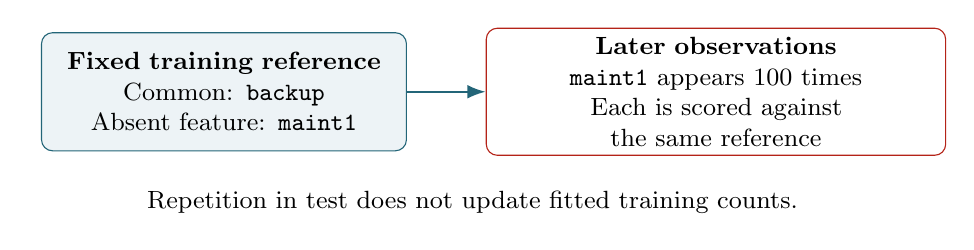
\begin{tikzpicture}[font=\small,>=Latex]
\node[draw=accent,fill=pale,rounded corners,text width=4.4cm,align=center,minimum height=1.5cm] (train) {\textbf{Fixed training reference}\\Common: \tok{backup}\\Absent feature: \tok{maint1}};
\node[draw=reviewred,rounded corners,text width=5.6cm,align=center,minimum height=1.5cm,right=1.0cm of train] (test) {\textbf{Later observations}\\\tok{maint1} appears 100 times\\Each is scored against the same reference};
\draw[->,thick,color=accent] (train) -- (test);
\node[text width=11cm,align=center,below=0.35cm of $(train.south)!0.5!(test.south)$] {Repetition in test does not update fitted training counts.};
\end{tikzpicture}
\caption{Illustration of the fixed-reference novelty score. High scores become flags only when retained features and the saved threshold permit them. This is an explanatory scenario, not a measured detection result.}
\label{fig:novelty-reference}
\end{figure}

\begin{table}[H]
\centering\small
\begin{tabular}{lll}
\toprule
\textbf{Time} & \textbf{Illustrative authentication activity} & \textbf{Interpretation} \\
\midrule
08:00:00 & \tok{backup}: public-key login & Familiar reference activity \\
08:00:03 & \tok{backup}: disconnect & Surrounding context \\
08:05:00 & \tok{backup}: public-key login & Familiar reference activity \\
08:05:03 & \tok{backup}: disconnect & Surrounding context \\
\rowcolor{reviewred!7}
\textcolor{reviewred}{\textbf{08:10:00}} & \textcolor{reviewred}{\textbf{\tok{maint1}: public-key login}} & \textcolor{reviewred}{\textbf{Candidate for review}} \\
08:10:03 & \tok{maint1}: disconnect & Surrounding context \\
\bottomrule
\end{tabular}
\caption{Chronological example: the highlighted login explains a possible rarity finding. Red indicates attention, not a confirmed attack. A session-level finding can include both the login and disconnect.}
\label{tab:novelty-example}
\end{table}

For completeness, let \(n_j\) be the number of training observations activating retained rarity feature \(j\), and let \(N\) be the training population. Both current implementations use \(\alpha=0.5\):
\begin{equation}
\label{eq:token-novelty}
p_j=\frac{n_j+\alpha}{N+2\alpha},\qquad
s_{\mathrm{novelty}}(x)=\max_{j:x_j\ne0}\left[-\ln p_j\right].
\end{equation}
An observation with no active rarity features receives zero. The implementation clips probabilities before taking the logarithm and separately counts active features with zero training presence. The score is compared with its saved threshold; it is not an attack probability. A hash collision, feature removal or calibration tie can keep a genuinely new behaviour below the alert boundary. If the regime change already dominates validation, its tied scores can influence calibration before testing begins.

\subsection{Feature Selection and Ensembles}\label{sec:selection}

The model zoo trains every family twice per view: on the full Phase 3 matrix and on a selected subset of its columns. Selection reads only the training and validation splits and runs six steps in order; a feature removed at one step is not considered again.

\begin{enumerate}
\item \textbf{Identity exclusion.} Columns whose names contain a row, record, event, line, session, episode or dataset identifier, or the raw epoch timestamp, are removed first, so that no model can separate observations by their position in the data; the OSSEC list also names process identifiers, agent counters and raw ports. In the current matrices only AUTH individual lines are affected: the epoch timestamp and its log twin are removed. The other columns on the lists never reach the matrices.
\item \textbf{Constant features.} On a random sample of 100,000 training rows, a feature whose standard deviation is below \(10^{-9}\) is removed. Most such features are hashed columns into which no token of the sample fell.
\item \textbf{Drift between training and validation.} For each remaining feature \(j\), the two-sample Kolmogorov--Smirnov statistic compares its distribution in the training sample with a random sample of 100,000 validation rows:
\begin{equation}
\label{eq:18}
D_j=\sup_v\bigl|\widehat{F}_{j,\mathrm{train}}(v)-\widehat{F}_{j,\mathrm{val}}(v)\bigr|,
\end{equation}
where \(\widehat{F}\) is the empirical cumulative distribution. A feature with \(D_j>0.25\) is removed, because a threshold calibrated on validation data would rest on a feature whose behaviour had already changed.
\item \textbf{Redundancy.} Pearson correlations are computed between the remaining features on the training sample. Features are visited in matrix order; any later feature whose absolute correlation with a kept earlier feature exceeds 0.98 is removed, and the earlier one stays. A count and its log twin are often removed this way.
\item \textbf{Importance.} An Isolation Forest of 100 trees is fitted to the training sample's remaining features. Its anomaly score \(s(x)\), oriented so that larger means more unusual, is computed for up to 10,000 validation rows. For each feature \(j\), that feature's column is shuffled across the rows, \(x^{(\pi_j)}\), the other columns are left unchanged, and the importance is the mean absolute change in score:
\begin{equation}
\label{eq:19}
I_j=\frac{1}{n}\sum_{i=1}^{n}\bigl|\,s(x_i^{(\pi_j)})-s(x_i)\bigr|.
\end{equation}
A feature that the forest does not use for its splits leaves the scores unchanged and receives an importance near zero.
\item \textbf{Cut-off.} Features are ranked by importance, \(I_{(1)}\ge I_{(2)}\ge\cdots\), and the smallest number covering 95\% of the total importance is kept, bounded below by 10 and above by 150:
\begin{equation}
\label{eq:20}
k^*=\min\Bigl\{k:\textstyle\sum_{r\le k}I_{(r)}\big/\sum_{r}I_{(r)}\ge0.95\Bigr\},\qquad k=\min\bigl(150,\max(10,k^*)\bigr).
\end{equation}
\end{enumerate}

Table~\ref{tab:selection} gives the number of features before and after selection for every view that has a model zoo, with the number removed at each step.

\begingroup
\footnotesize
\begin{longtable}{>{\RaggedRight\arraybackslash}p{\dimexpr 0.22\linewidth-2\tabcolsep\relax}>{\RaggedLeft\arraybackslash}p{\dimexpr 0.10\linewidth-2\tabcolsep\relax}>{\RaggedLeft\arraybackslash}p{\dimexpr 0.10\linewidth-2\tabcolsep\relax}>{\RaggedLeft\arraybackslash}p{\dimexpr 0.11\linewidth-2\tabcolsep\relax}>{\RaggedLeft\arraybackslash}p{\dimexpr 0.09\linewidth-2\tabcolsep\relax}>{\RaggedLeft\arraybackslash}p{\dimexpr 0.12\linewidth-2\tabcolsep\relax}>{\RaggedLeft\arraybackslash}p{\dimexpr 0.12\linewidth-2\tabcolsep\relax}>{\RaggedLeft\arraybackslash}p{\dimexpr 0.14\linewidth-2\tabcolsep\relax}}
\caption{Features before and after selection, and the number removed at each step}\label{tab:selection}\\
\toprule
\rowcolor{pale} \textbf{View} & \textbf{Before} & \textbf{Identity} & \textbf{Constant} & \textbf{Drift} & \textbf{Redundant} & \textbf{Below cut-off} & \textbf{After} \\
\midrule
\endfirsthead
\multicolumn{8}{l}{\small\itshape Table \thetable{} --- continued}\\
\toprule
\rowcolor{pale} \textbf{View} & \textbf{Before} & \textbf{Identity} & \textbf{Constant} & \textbf{Drift} & \textbf{Redundant} & \textbf{Below cut-off} & \textbf{After} \\
\midrule
\endhead
\midrule
\multicolumn{8}{r}{\footnotesize Continued on the next page}\\
\endfoot
\bottomrule
\endlastfoot
AUTH individual lines & 785 & 2 & 404 & 0 & 167 & 172 & \textbf{40} \\[3pt]
AUTH sessions & 573 & 0 & 210 & 0 & 78 & 217 & \textbf{68} \\[3pt]
AUTH 5-minute windows & 603 & 0 & 120 & 6 & 39 & 320 & \textbf{118} \\[3pt]
AUTH daily behaviour & 603 & 0 & 166 & 0 & 37 & 250 & \textbf{150} \\[3pt]
OSSEC individual lines & 790 & 0 & 161 & 0 & 87 & 392 & \textbf{150} \\[3pt]
OSSEC episodes & 647 & 0 & 333 & 18 & 123 & 116 & \textbf{57} \\[3pt]
OSSEC 5-minute windows & 695 & 0 & 270 & 25 & 78 & 246 & \textbf{76} \\[3pt]
OSSEC daily behaviour & 681 & 0 & 272 & 34 & 45 & 192 & \textbf{138} \\[3pt]
\end{longtable}
\endgroup

Source: each view's \projectref{feature decisions}{data/phase4_detection/<source>/model_zoo/<view>/feature_relevance.csv}. AUTH daily behaviour and OSSEC individual lines reach the upper bound of 150, so features beyond it are cut although the 95\% coverage had not yet been reached. PF and IPFilter have no model zoo and therefore no selected feature set.

Selection can reduce duplicate or uninformative inputs, but it is not supervised identification of attack-causing features. Importance measures how much one Isolation Forest's score depends on a feature, from one random shuffle per feature; correlated features share their importance, and a feature the forest ignores can still matter to another family.

\textbf{Screening the models.} Each model is then checked on the validation split for five failure modes. Its alert threshold is first set at the larger of the 99.5th percentile of its validation scores and the score that keeps alerts within a cap (1\% of observations for individual lines, 5\% otherwise), raised slightly when tied scores would exceed the cap. With \(n\) validation observations, \(E=\max(0.005\,n,1)\) alerts expected at the 99.5th percentile, and \(A_m\) the observations that model \(m\) flags, the checks in Table~\ref{tab:screening} run in order, and a model is removed at the first one it fails.

\begingroup
\small
\begin{longtable}{>{\RaggedRight\arraybackslash}p{\dimexpr 0.22\linewidth-2\tabcolsep\relax}>{\RaggedRight\arraybackslash}p{\dimexpr 0.48\linewidth-2\tabcolsep\relax}>{\RaggedRight\arraybackslash}p{\dimexpr 0.30\linewidth-2\tabcolsep\relax}}
\caption{Model screening checks, in the order applied}\label{tab:screening}\\
\toprule
\rowcolor{pale} \textbf{Failure mode} & \textbf{How it is measured} & \textbf{A model is removed when} \\
\midrule
\endfirsthead
\multicolumn{3}{l}{\small\itshape Table \thetable{} --- continued}\\
\toprule
\rowcolor{pale} \textbf{Failure mode} & \textbf{How it is measured} & \textbf{A model is removed when} \\
\midrule
\endhead
\midrule
\multicolumn{3}{r}{\footnotesize Continued on the next page}\\
\endfoot
\bottomrule
\endlastfoot
Invalid scores & The share of validation scores that are finite numbers. & Fewer than 99\% are finite. \\[3pt]
Insufficient alert production & The alert fill \(|A_m|/E\): how many of the expected alerts the model actually produces. Many tied scores at the threshold make it small. & The fill is below 0.5. \\[3pt]
Unstable validation behaviour & The validation split is cut at its chronological midpoint, and the model's alert rates \(a_1\) and \(a_2\) in the two halves give the ratio \(\rho=\max(a_1,a_2)/\max(\min(a_1,a_2),\,1/\lfloor n/2\rfloor)\). Checked only when \(n\ge2{,}000\) and \(E/2\ge10\), so that each half expects at least ten alerts. & \(\rho>3\): one half of the validation period has more than three times the other's alert rate. \\[3pt]
Very isolated alert set & The Jaccard agreement with every other model, \(J(A_m,A_o)=|A_m\cap A_o|/|A_m\cup A_o|\). & Its highest agreement with any other model is below 0.05. \\[3pt]
Near-duplicate ranking & Spearman rank correlation of the validation scores of the models still in, on up to 200,000 sampled rows. Models are visited in descending order of their mean agreement with the others. & Its rank correlation with an already kept model exceeds 0.95; the kept model stays. \\[3pt]
\end{longtable}
\endgroup

Two more rules complete the ensemble. If fewer than two models remain, those removed as unstable, isolated or near-duplicate are put back; models with invalid scores or too few alerts are not. Then, where proxy labels exist (see below), models are added one at a time, each time choosing the one that most raises the proxy detection rate of the averaged percentile score at a fixed budget of \(0.005\,n\) alerts. The ensemble keeps the shortest such list that has at least two models and comes within 0.005 of the best detection rate; the rest are recorded as adding little detection.

In the current runs, every view's two ensembles keep two models except the AUTH 5-minute selected-feature ensemble, which keeps ten. Most removals are for little detection gain. Eight of the sixteen ensembles (both feature sets of AUTH sessions, AUTH 5-minute windows, OSSEC episodes and OSSEC 5-minute windows) also lose models to the stability check; the full-feature ensembles of OSSEC daily behaviour and individual lines lose models to the invalid-score or alert-production checks; and AUTH daily behaviour (both sets) and OSSEC individual lines (full set) each lose one model with an isolated alert set. Source: each view's \projectref{ensemble membership}{data/phase4_detection/<source>/model_zoo/<view>/<feature set>/ensemble_membership.csv}. Agreement is an engineering heuristic: several models can share the same blind spot because they see the same data and features.

An ensemble score puts each member's score on a common scale through its training-score distribution and averages them:

\begin{equation}
\label{eq:7}
u_m(x)=\widehat{F}_{m,\mathrm{train}}(s_m(x)),\qquad
s_{\mathrm{ens}}(x)=\frac{1}{M}\sum_{m=1}^{M}u_m(x).
\end{equation}

Consensus alerts are a separate output: an observation is flagged when at least three members flag it, or all members when there are fewer than three.

Some selection steps use \textbf{proxy-positive observations}. For AUTH, an individual line is proxy-positive when its event type is one of 37 security-related types, such as failed or invalid logins, PAM and \nolinkurl{su} events, and key-exchange or protocol errors; an aggregate observation is proxy-positive when any of its failure, invalid-user, access-denied, privilege, protocol-error or PAM-error counts is non-zero. For OSSEC, the equivalents are agent stops, manager-communication failures, integrity-baseline and configuration gaps, and severities of ERROR or higher. The proxy detection rate is the share of proxy-positive validation observations caught within a fixed alert budget. Proxies check whether a model finds recognisable behaviour; they are not verified attack labels, and a field named \nolinkurl{detection_rate} measures recovery of proxies, not attack recall.

\textbf{Relation to AutoML, and the natural extension.} In automated machine learning (AutoML) terms, the model zoo already has:
\begin{itemize}
\item a search space of thirteen families and two feature sets per view;
\item automated feature selection;
\item model screening by label-free checks;
\item greedy forward ensemble selection against an objective, here the proxy detection rate at a fixed budget.
\end{itemize}
Supervised AutoML systems combine such search with hyperparameter optimisation and stacked ensembles; AutoGluon had the highest average performance across the nine frameworks of the AMLB benchmark \cite{ref14}. Two parts are missing here. Hyperparameters are fixed per family (for example 300 trees for Isolation Forest and \(\nu=0.05\) for the RBF one-class SVM), and the objective is a proxy rather than labelled attacks.

The extension has two stages:
\begin{itemize}
\item \textbf{Before labels.} Meta-learned selection and tuning learn which detectors and settings work from their performance on benchmark corpora \cite{ref15,ref19}. The screening checks above are internal criteria of the kind a large study found rarely beat a sound default \cite{ref16}. Any label-free tuning should therefore be judged against reviewed outcomes, and benchmark corpora resemble SSH session features poorly.
\item \textbf{After the hypothesis register yields labels} (Appendix~\ref{app:hypotheses}). A supervised decision model becomes possible. Gradient-boosted trees on the Phase 3 features with the unsupervised scores as extra inputs follow the XGBOD pattern \cite{ref17}. Tabular foundation models suit the small labelled sets expected first \cite{ref18}. Both should be tuned and evaluated on the chronological split and compared with the unsupervised ensemble. The limiting resource is the labels, not the search.
\end{itemize}

\subsection{Sequential Patterns and Association Rules}\label{sec:seqmethods}

A pattern \(p=(p_1,\ldots,p_r)\) is a subsequence of a sequence \(s=(k_1,\ldots,k_L)\) if its tokens appear in \(s\) in the same order, possibly with other tokens between them. Its support is the share of observations that contain it:

\begin{equation}
\label{eq:8}
\operatorname{supp}(p)=\frac{1}{N}\sum_{i=1}^{N}\mathbf{1}[p\preceq s_i].
\end{equation}

A pattern repeated inside one session still counts once. Identical sequences are stored once with a count, which gives the same result faster.

PrefixSpan finds frequent patterns by growing them one token at a time from a prefix, searching only the sequences that contain that prefix instead of listing every possible pattern. Pei et al.\ (2001) introduced it \cite{ref4}; here it builds the routine catalogue. A sequential rule's confidence is

\begin{equation}
\label{eq:9}
\operatorname{conf}(A\Rightarrow b)=
\frac{\#\{s:A\mathbin{\|}b\preceq s\}}{\#\{s:A\preceq s\}},
\end{equation}

where \(A\mathbin{\|}b\) is \(A\) followed by \(b\). A high-confidence rule says what usually follows; it says nothing about cause, immediacy or elapsed time.

To explain where a detector's alerts concentrate, the alert profile uses \textbf{FP-growth}, short for \emph{frequent-pattern growth}, on \textbf{unordered} sets of attributes. FP-growth finds every combination of attributes that occurs often enough by storing the data once in a compressed prefix tree, the \emph{frequent-pattern tree}, and reading combinations from it, instead of generating candidate combinations and counting each one. For an attribute set \(A\) and an alert indicator \(Y\), lift is

\begin{equation}
\label{eq:10}
\operatorname{lift}(A\Rightarrow Y)=\frac{P(Y\mid A)}{P(Y)}.
\end{equation}

Lift above one means alerts are more common in that population than overall, which exposes a detector dominated by one host family or message type. Han et al.\ (2004) introduced FP-growth \cite{ref5}, and the mlxtend contributors document the support, confidence and lift measures used here \cite{ref6}.

\subsection{Visualisation and Analyst Interpretation}

t-SNE, introduced by van der Maaten and Hinton (2008) \cite{ref7}, and UMAP, introduced by McInnes, Healy and Melville (2018) \cite{ref8}, draw high-dimensional observations in two dimensions. Both keep neighbours together better than they keep long distances, so the maps are for exploring structure, not for measuring how different two behaviours are.

Groups are found by HDBSCAN on the t-SNE map, a density-based method whose implementation McInnes, Healy and Astels (2017) described \cite{ref9}; remaining observations are assigned by neighbour votes in a saved higher-dimensional embedding. Because the projection shapes the groups, a group helps navigation and batch review; it is not a security verdict.

\clearpage
\section{Detailed Implementation and Analyst Workflow}
\label{app:implementation}

\subsection{Architecture and Processing Flow}

Project DAD (Data Anomaly Detection) Console separates batch analytics from interactive investigation. Python pipeline phases produce observations, features, models, scores and evidence; a local Python service and a TypeScript interface present them; SQLite stores hold events, reviews and reports. The service listens on \nolinkurl{127.0.0.1:8765}.

The pipeline runs as numbered phases, each reading the previous phase's saved output. Table~\ref{tab:phases} lists them with the station names used on the console's Documentation page, and follows one invented authentication line through them.

\begingroup
\small
\begin{longtable}{>{\RaggedRight\arraybackslash}p{\dimexpr 0.09\linewidth-2\tabcolsep\relax}>{\RaggedRight\arraybackslash}p{\dimexpr 0.16\linewidth-2\tabcolsep\relax}>{\RaggedRight\arraybackslash}p{\dimexpr 0.36\linewidth-2\tabcolsep\relax}>{\RaggedRight\arraybackslash}p{\dimexpr 0.39\linewidth-2\tabcolsep\relax}}
\caption{Pipeline phases, with an invented line followed through them}\label{tab:phases}\\
\toprule
\rowcolor{pale} \textbf{Phase} & \textbf{Name} & \textbf{What it does} & \textbf{Example} \\
\midrule
\endfirsthead
\multicolumn{4}{l}{\small\itshape Table \thetable{} --- continued}\\
\toprule
\rowcolor{pale} \textbf{Phase} & \textbf{Name} & \textbf{What it does} & \textbf{Example} \\
\midrule
\endhead
\midrule
\multicolumn{4}{r}{\footnotesize Continued on the next page}\\
\endfoot
\bottomrule
\endlastfoot
0 & Raw logs & Keeps the monthly archives copied from the servers, unchanged. & The July archive of \tok{host-a} contains \tok{Jul 14 16:20:37 host-a sshd[2785]: Failed password for invalid user maint1 from 192.0.2.17 port 50123 ssh2}. \\[3pt]
1 & Classify & Matches every line against written rules and gives it an event type and fields; lines that no rule fits are kept as unknown. & The line becomes one row: event type \tok{SSH_INVALID_USER}, user \tok{maint1} and source address \tok{192.0.2.17}, with its archive, file and line number. \\[3pt]
2 & Observations & Groups the rows the ways an analyst looks at them: single lines, login sessions or OSSEC episodes, five minutes on one server, and a whole day on one server. & The row is an observation of its own, and also part of a session, of the 16:20--16:25 window and of 14 July on \tok{host-a}. \\[3pt]
2c & Coverage & Records which servers sent logs on which days, so that gaps are not mistaken for quiet days. & 14 July is marked as a day with logs for \tok{host-a}. \\[3pt]
3 & Describe & Turns each observation into numbers (counts, times and hashed words) and places it in the training, validation or test period. & The session becomes a row of 573 numbers, such as one failure, a duration of seven seconds and the hour 16, in the test period. \\[3pt]
4 & Detectors & Scores every observation: robust deviation, Isolation Forest and novelty (4a); the model zoo (4b); the maps (4c); silent servers (4d); accounts and addresses seen for the first time (4e); and routines and sequence surprise (4f). & A rare user name and an unusual first step can give the session high novelty and sequence scores; \tok{maint1} on \tok{host-a} is listed as first seen. \\[3pt]
5 & Evidence & Traces every flag back to the original lines. & The flag links back to the archive, file and line number of the line above. \\[3pt]
6 & Report & Writes an offline web report per log type. & The session appears among the AUTH report's findings. \\[3pt]
7 & Alerts & Collects everything flagged into one ranked list per log type; 7b groups similar observations and 7c gathers what the other logs say about the same addresses and servers. & The session joins a group of invalid-user sessions; 7c shows whether \tok{192.0.2.17} also appears in the firewall logs. \\[3pt]
8 & Learn from reviews & Planned: a classifier that learns from reviewed decisions. & Not yet run; it needs reviewed examples. \\[3pt]
9 & AI triage & A small local language model suggests a category and its reasons for flagged lines; a person decides. & The suggestion is \emph{security relevant}, citing the invalid user; the analyst confirms or overrides it in Review. \\[3pt]
\end{longtable}
\endgroup

The console's pattern workbench sits beside Phase 1: it measures and extends parsing coverage for new or changed formats, but its rules reach the pipeline only through a manual change to Phase 1 (Section~\ref{sec:patterns}). Phases 8 and 9 have important maturity limits, described in Section~\ref{sec:localai}.

Every phase keeps its intermediate results, and each score links back to the parsed events and to the original archive, file and line. Had the example line been given the wrong event type, the analyst could follow its flag back to the line and see the mistake. Figure~\ref{fig:architecture} shows the whole flow.

\begin{figure}[p]
\centering
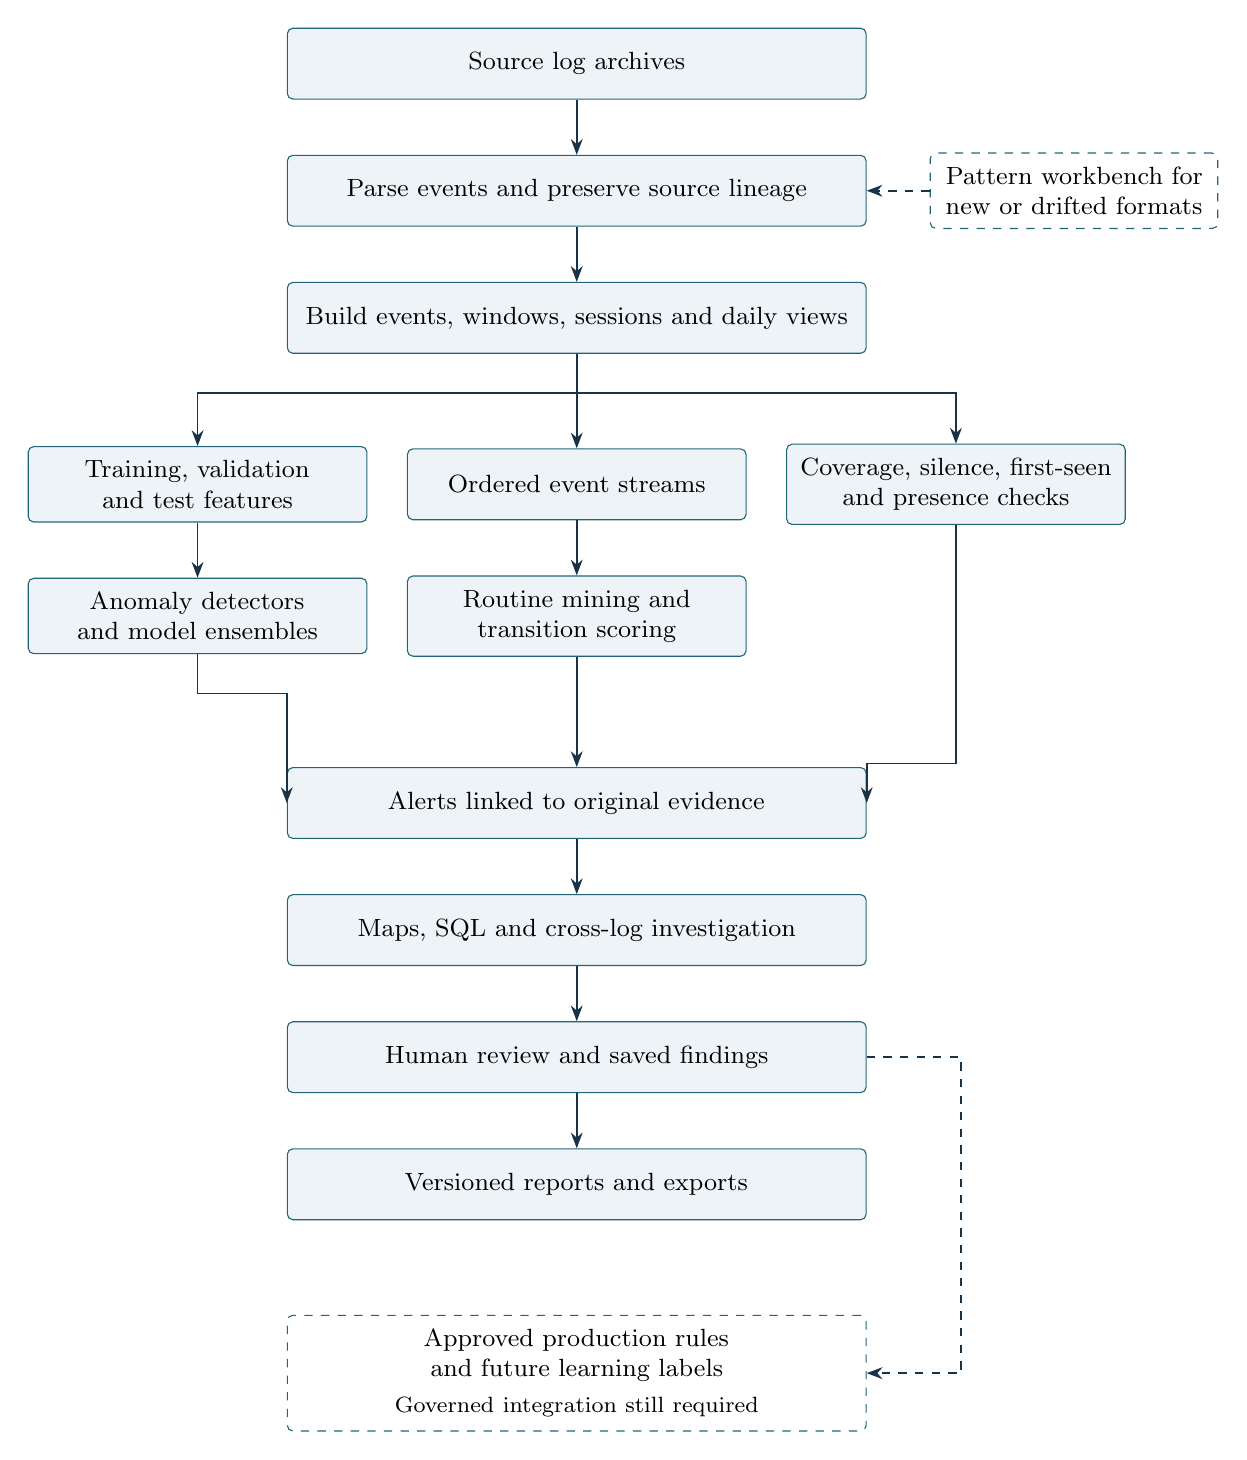
\begin{tikzpicture}[
  node distance=7mm and 5mm,
  box/.style={draw=accent,rounded corners=2pt,fill=pale,align=center,
    text width=3.95cm,minimum height=9mm,inner sep=5pt,font=\small},
  wide/.style={box,text width=7cm},
  flow/.style={-{Stealth[length=2mm]},draw=ink,semithick}
]
\node[wide] (a) {Source log archives};
\node[wide,below=of a] (b) {Parse events and preserve source lineage};
\node[box,right=8mm of b,text width=3.3cm,dashed,fill=white] (p) {Pattern workbench for new or drifted formats};
\node[wide,below=of b] (c) {Build events, windows, sessions and daily views};
\node[box,below=12mm of c] (f) {Ordered event streams};
\node[box,left=of f] (d) {Training, validation and test features};
\node[box,right=of f] (h) {Coverage, silence, first-seen and presence checks};
\node[box,below=of d] (e) {Anomaly detectors and model ensembles};
\node[box,below=of f] (g) {Routine mining and transition scoring};
\node[wide,below=14mm of g] (i) {Alerts linked to original evidence};
\node[wide,below=of i] (j) {Maps, SQL and cross-log investigation};
\node[wide,below=of j] (k) {Human review and saved findings};
\node[wide,below=of k] (l) {Versioned reports and exports};
\node[wide,below=12mm of l,dashed,fill=white] (m) {Approved production rules and future learning labels\\[2pt]
  {\footnotesize Governed integration still required}};
\draw[flow] (a)--(b);
\draw[flow] (b)--(c);
\draw[flow] (c)--(f);
\draw[flow] (c.south)--++(0,-5mm)-|(d.north);
\draw[flow] (c.south)--++(0,-5mm)-|(h.north);
\draw[flow] (d)--(e);
\draw[flow] (f)--(g);
\draw[flow] (g)--(i);
\draw[flow] (e.south)--++(0,-5mm)-|(i.west);
\draw[flow] (h.south)|-([yshift=5mm]i.east)--(i.east);
\draw[flow] (i)--(j);
\draw[flow] (j)--(k);
\draw[flow] (k)--(l);
\draw[flow,dashed] (k.east)--++(12mm,0)|-(m.east);
\draw[flow,dashed] (p.west)--(b.east);
\end{tikzpicture}
\caption{Processing and investigation architecture. Dashed paths identify integration that remains unfinished: rules from the pattern workbench are adopted into parsing manually, and governed production rules and learning labels are not yet integrated.}
\label{fig:architecture}
\end{figure}
\FloatBarrier

\subsection{Source-Specific Preparation and Data Quality}

The study covers August 2025 to July 2026. AUTH and OSSEC provide the main behavioural baselines, across fifteen hosts. AUTH holds authentication activity; the OSSEC source is mostly the agent's own operational log, not a full record of host intrusion alerts.

PF and IPFilter activity is sparse or concentrated in a short period, so they are processed differently: time slots, connection attempts and flow episodes record when activity exists against a mostly quiet baseline. They have no model zoo or maps.

\textbf{Example: why sparse sources need presence views.} All 52,231 IPFilter lines fall in November 2025, and the other eleven monthly files are empty. A model of daily counts would learn that a normal day has zero lines and score the whole of November as one long anomaly, without saying which hours matter. The presence view instead divides the year into 5-minute, hourly and daily slots and asks of each slot whether anything happened and what: of PF's 1,471,680 five-minute slots, only 410 contain activity, and those are the ones an analyst reviews.

Coverage processing marks each server-day as active, quiet with support from another log, a collection gap, or unknown. An empty firewall file can mean no blocked traffic; missing agent messages can mean something else. Neither missing data nor an absence of flags shows that a system was secure.

\textbf{Example: reading an empty day.} Suppose the firewall log of an invented host \tok{host-a} is empty on 3 March. If \tok{host-a}'s authentication log shows logins that day, the host was running and logging, and the empty firewall file is consistent with no blocked traffic: a supported quiet day. If neither log has anything for 3 March, the day's availability is unknown, and the absence of alerts says nothing about it. Likewise, an OSSEC agent that normally reports every few minutes and falls silent for six hours on a working day is a candidate for the silence check (Phase 4d), because logging may have been switched off.

Unrecognised lines are tracked as a data-quality problem, never treated as normal. Two leftover PF capture files from 2022--2024 are excluded from the study period: choosing sources is part of the method, not a preprocessing detail. The pattern workbench (Section~\ref{sec:patterns}) measures and reduces the problem for new inputs.

\subsection{Onboarding New Log Formats: Pattern Discovery}
\label{sec:patterns}

Every later phase depends on Phase 1 recognising a line. Phase 1 uses hand-written regular expressions: one for a source's line head (time, host and process) and an ordered list for its messages, each naming an event type (all of them are listed in the Appendices). A line that matches none is unrecognised and contributes nothing to observations, features or alerts. This happens when a new source arrives, such as a database audit export, and when an upgrade changes the wording of a known one. The console's pattern workbench, \emph{Patterns}, lets an analyst measure the gap and write the missing rules without editing code, in passes: read the lines, see what is still unknown, add a rule, read them again.

\textbf{A worked example.} The screens of Section~\ref{sec:guide} (Figures~\ref{fig:patterns-table} to~\ref{fig:patterns-regex}) show the following session, run on a made-up export from a RADIUS authentication server that the pipeline has no rules for.

\begin{enumerate}
\item \textbf{Input.} The export is a CSV file of 450 rows with the columns \tok{_time}, \tok{host}, \tok{port}, \tok{client_ip}, \tok{sourcetype} and \tok{_raw}. The workbench checks that the first 100 rows have a header and the same number of values, and shows each column's type and first values. The analyst chooses \tok{_raw} as the raw log line and leaves out \tok{port}.
\item \textbf{First pass.} No Phase 1 rule recognises a RADIUS line, so coverage, the share of lines with an event type, is 0\%:
\begin{equation}
\label{eq:15}
C=\frac{n_1+n_R}{N},
\end{equation}
where \(N\) is the number of lines and \(n_1\) and \(n_R\) are those named by Phase 1 and by workbench rules.
\item \textbf{Shapes.} The workbench masks the parts of each line that vary, such as times, numbers and addresses, and groups lines whose masks are alike. Every line begins with a head of the shape \tok{<time> nas-<n> radiusd[<number>]:}, so that is offered as a candidate prefix. The messages \tok{Login OK: [user1] (from client sw1 port 1)} and \tok{Login incorrect: [user5] (from client sw1 port 5)} differ only in their second and third words, so they fall into one shape, \tok{Login * * (from client sw1 port <number>)}. A shape \tok{Rejected ignored request from <IP> port <number> - ID <number>} appears only from 7 July and is marked \emph{new}.
\item \textbf{Prefix rule.} The analyst adds the head shape, accepts the suggested expression, which names the time, host name and process number, and saves it. On the next pass all 450 lines are cut by the prefix, but none is named yet.
\item \textbf{Message rule.} From six \emph{Login} examples the workbench offers three candidates (Figure~\ref{fig:patterns-regex}). \emph{Exact} and \emph{Fields} match all six examples and are estimated to match about 112 lines; \emph{Start}, \nolinkurl{Login(?:\s+(?P<rest>.*))?}, would match about 400 but names nothing inside the message. The estimate comes from a random sample of the unnamed lines: if \(k\) of \(m\) sampled lines match and \(U\) lines are unnamed,
\begin{equation}
\label{eq:16}
\hat{N}=U\cdot\frac{k}{m}.
\end{equation}
The analyst saves \emph{Exact} as event type \tok{RADIUS_LOGIN}.
\item \textbf{Second pass.} Coverage rises to 24.9\%: 112 lines named, 338 cut by the prefix only and none unknown (Figure~\ref{fig:patterns-coverage}). The estimate was exact this time, and it also shows why only a quarter of the lines were named: the chosen expression kept the literal word \tok{sw0} from the examples. Replacing \tok{sw0} with a named group, \nolinkurl{(?P<client>\w+)}, would name all 400 login lines on the next pass.
\item \textbf{Export.} The rules are exported as JSON or as lines for Phase 1's rule list. Adopting them is a manual, reviewed change to Phase 1.
\end{enumerate}

Table~\ref{tab:workbench} summarises the remaining behaviour.

\begingroup
\small
\begin{longtable}{>{\RaggedRight\arraybackslash}p{\dimexpr 0.22\linewidth-2\tabcolsep\relax}>{\RaggedRight\arraybackslash}p{\dimexpr 0.78\linewidth-2\tabcolsep\relax}}
\caption{The pattern workbench at a glance}\label{tab:workbench}\\
\toprule
\rowcolor{pale} \textbf{Aspect} & \textbf{Behaviour} \\
\midrule
\endfirsthead
\multicolumn{2}{l}{\small\itshape Table \thetable{} --- continued}\\
\toprule
\rowcolor{pale} \textbf{Aspect} & \textbf{Behaviour} \\
\midrule
\endhead
\midrule
\multicolumn{2}{r}{\footnotesize Continued on the next page}\\
\endfoot
\bottomrule
\endlastfoot
Inputs & Pasted or uploaded lines, or a file, folder, ZIP or gzip archive on the laptop; up to five million lines per pass. CSV and Excel tables need a raw-log column; the older \nolinkurl{.xls} format is refused. \\[3pt]
Rule kinds & Prefixes remove a line's head; suffixes remove a trailing token such as \nolinkurl{[preauth]}; message rules name an event type when they match the rest of the line completely, ignoring case as Phase 1 does. Phase 1's own rules are tried first. \\[3pt]
Shapes & Lines with the same number of tokens are merged, largest group first, when they differ in at most \(\min(2,\lfloor n/3\rfloor)\) of their \(n\) tokens. He et al.\ (2017) detailed Drain, a log parser that groups messages into templates with a fixed-depth tree \cite{ref11}; this is a simpler heuristic in the same spirit. \\[3pt]
Drift markers & A shape first seen in the last quarter of the period is marked \emph{new}; a rule whose last match is earlier than that is marked \emph{quiet}. Coverage over time shows a fall from the date a format changed. Both point to possible drift; neither establishes it. \\[3pt]
Suggestions & Up to four candidates: \emph{Exact} (token by token), \emph{Fields} (whitespace-separated fields), \emph{Anchors} (the fields shared by every example, in order; offered when the examples differ in length) and \emph{Start} (the shared first words and an open remainder). Variable parts become named groups, using Phase 1's field names where the neighbouring word makes the meaning clear, such as \nolinkurl{source_ip} after ``from''. \\[3pt]
Estimates & Candidates are tried on a uniform random sample of the unnamed lines, kept by reservoir sampling as Vitter (1985) described it \cite{ref12}, so the sample stays uniform while the lines stream past. The next pass gives the exact count. \\[3pt]
Safety & A rule must compile in Python's \nolinkurl{re} module, which Phase 1 uses, and must not nest one unbounded repetition in another, such as \nolinkurl{(a+)+}, whose matching time can grow exponentially on lines that almost match. Each match is limited to 50 milliseconds; a rule that exceeds it is set aside for the rest of the pass. \\[3pt]
Storage and audit & Rules are stored in the console's own database with up to five examples, whose IPv4 addresses are replaced by documentation addresses. Every save, change, deletion and export is written to the activity log. \\[3pt]
Adoption & Neither Analyze nor the pipeline reads workbench rules yet. Adopting one is a manual change to Phase 1, and a new log type also needs its own observation, feature and detection stages before it can be scored. \\[3pt]
Deletion & Log types created in the workbench are listed as unapproved; any user may delete one without signing in, because only the workbench's records are removed (decision Q34). Adding datasets and training still require an administrator. \\[3pt]
Unknown-format check & In Simple mode, the first 200 lines of an upload are checked against Phase 1. Below 5\% recognised, the analysis stops and offers the workbench, so that a result of nothing unusual is not read as covering lines the parser could not read. \\[3pt]
\end{longtable}
\endgroup

\subsection{Temporal Evaluation and Alert Calibration}\label{sec:temporal}

Each view is split in time order into about 70\% training, 15\% validation and 15\% test, with purge gaps at the boundaries. The split divides observations, not calendar time, so boundaries differ by source and view; exact counts and dates are saved per view.

Training fits the transformations and models; validation chooses models and alert thresholds; the test period shows how those fixed choices behave on later data. This mirrors live monitoring better than a random split, though it cannot compensate for unknown attacks or unrecorded changes in the history.

Each primary detector's validation alert budget is the smaller of a daily target times the number of validation days and a fixed share of the validation observations, subject to minimum-size rules. When tied scores straddle the budget, the threshold moves up so that the whole tied group is not flagged.

\textbf{Example.} Suppose a sessions view holds 1,000,000 observations in time order. The first 700,000 form the training period, the next 150,000 validation and the last 150,000 the test period. Sessions that start within 15 minutes either side of a boundary are left out of both periods (the purge gap; 5 minutes for 5-minute windows, a day for daily views, none for single lines), so that one session cannot sit in two periods. If validation spans 50 days, the sessions view's target of 10 alerts a day permits \(10\times50=500\) validation alerts, and its population cap of 5\% permits 7,500; the smaller number, 500, applies. The threshold is the score of the 500th most unusual validation session. If that score is shared by the 495th to the 520th sessions, flagging all of them would give 520 alerts, so the threshold is raised just above the shared score and 494 sessions are flagged instead.

These targets apply \textbf{per detector and per view}. They are not one shared alert allowance and do not cap any future day: a changed test period can exceed the validation workload. The model zoo uses its own quantile and selection logic (Section~\ref{sec:selection}).

\subsection{Sequence Construction and Routine Mining}\label{sec:sequences}

The sequence feature rebuilds Phase 2's AUTH sessions and OSSEC episodes as complete event streams, keeping the same observation identities and splits. It improves the miner's input without changing how sessions are defined.

Events are ordered by time, then by file and line number. A line that appears in two overlapping files with the same time and text is kept once, with the second copy as an alias; genuine repeats within one file are kept. Consecutive repeats of an event type collapse into one token, with the run length kept beside it.

If events from different files share a second and cannot be ordered, the step between them is marked uncertain. Observations cut off at the start or end of the dataset (censored) are left out of training, and uncertain or cut-off steps are not scored.

\textbf{Example: building the sequences.} On an invented host, the line \tok{Accepted password for alice} at 09:00:05 appears both in \tok{auth.log} and in the rotated copy \tok{auth.log.1}, with the same time and text; the two copies become one event, and the second copy is kept as an alias so that either file can be shown as evidence. Three failed passwords in a row followed by a login become \tok{SSH_LOGIN_FAILED SSH_LOGIN_SUCCESS}, with the run length 3 kept beside the first token. If a disconnect from \tok{auth.log} and a login from another file carry the same second and cannot be ordered by line number, the step between them is marked uncertain.

\textbf{Example: support and rule confidence.} Take five invented sessions, written with short labels: \(L\) for \tok{SSH_LOGIN_SUCCESS}, \(F\) for \tok{SSH_LOGIN_FAILED}, \(D\) for \tok{SSH_DISCONNECT_RECEIVED}, \(U\) for \tok{SSH_USER_DISCONNECTED} and \(C\) for \tok{SSH_CONNECTION_CLOSED}.

\begin{center}
\small
\begin{tabular}{lll}
\toprule
\textbf{Session} & \textbf{Events after collapsing repeats} & \textbf{Contains \(L\) then \(U\)?} \\
\midrule
\(s_1\) & \(L\;D\;U\) & yes \\
\(s_2\) & \(F\;L\;D\;U\) & yes \\
\(s_3\) & \(L\;D\;U\) & yes \\
\(s_4\) & \(C\) & no \\
\(s_5\) & \(L\;D\) & no \\
\bottomrule
\end{tabular}
\end{center}

Sessions \(s_1\) and \(s_3\) are identical, so they are stored once with weight 2, which leaves four distinct sequences to mine but the same counts. The pattern \((L,U)\) occurs in \(s_1\), \(s_2\) and \(s_3\), with \(D\) between them, so its support (Equation~\ref{eq:8}) is \(3/5=60\%\). For the rule \(D\Rightarrow U\), four sessions contain \(D\) and three of them have \(U\) after it, so its confidence (Equation~\ref{eq:9}) is \(3/4=75\%\). That is below the 95\% required, so it is not kept as a high-confidence rule; in the real AUTH data the same rule holds in 100\% of 5,493,782 training sessions (Section~\ref{sec:routines-results}).

Table~\ref{tab:3} lists the mining settings. Every routine and rule they produced is listed in the Appendices.


\begingroup
\small
\begin{longtable}{>{\RaggedRight\arraybackslash}p{\dimexpr 0.28\linewidth-2\tabcolsep\relax}>{\RaggedRight\arraybackslash}p{\dimexpr 0.72\linewidth-2\tabcolsep\relax}}
\caption{Current routine-mining settings}\label{tab:3}\\
\toprule
\rowcolor{pale} \textbf{Setting} & \textbf{Current value and meaning} \\
\midrule
\endfirsthead
\multicolumn{2}{l}{\small\itshape Table \thetable{} --- continued}\\
\toprule
\rowcolor{pale} \textbf{Setting} & \textbf{Current value and meaning} \\
\midrule
\endhead
\midrule
\multicolumn{2}{r}{\footnotesize Continued on the next page}\\
\endfoot
\bottomrule
\endlastfoot
Token & Explicit event type \\[3pt]
Scope & Global and per host; a host catalogue requires at least 200 training observations \\[3pt]
Minimum support & At least 0.5\% of observations in scope and at least 20 observations \\[3pt]
Maximum pattern length & Eight tokens \\[3pt]
Pattern selection & Closed frequent subsequences within the configured search space, plus common whole-sequence summaries \\[3pt]
Rule confidence & At least 95\% \\[3pt]
Maximum rule antecedent & Three tokens \\[3pt]
Training exclusions & Censored observations; support exists for configured change windows, but none were applied in the recorded run \\[3pt]
\end{longtable}
\endgroup


Only closed patterns are kept: a shorter pattern is dropped when a longer one has exactly the same support. Global and per-host rows can describe the same pattern, so catalogue rows are not counts of distinct behaviours.

Two limits matter when turning routines into rules. Patterns allow other events between their steps, and no maximum time between steps is enforced. The catalogue and its rules also keep uncertain steps, which scoring leaves out, so patterns with ambiguous order need review before becoming policy. Phase 2's session boundaries remain heuristics, not verified user sessions.

\subsection{Transition Surprise: The Actual Sequence Alert Score}

PrefixSpan supplies the catalogue, but the sequence alert score is a \textbf{first-order transition-surprise score}: it asks how unlikely each step is, given the previous step, on that host. The Dashboard's short label for this detector is ``Frequent subsequences''.

For a previous event \(a\), next event \(b\) and host \(h\), host counts are smoothed towards all-host counts, and those towards \(b\)'s overall frequency:

\begin{equation}
\label{eq:11}
p_0(b)=\frac{C(b)+1}{\sum_v C(v)+|V|},
\end{equation}

\begin{equation}
\label{eq:12}
p_G(b\mid a)=\frac{C_G(a,b)+\beta p_0(b)}{C_G(a)+\beta},\qquad
p_h(b\mid a)=\frac{C_h(a,b)+\alpha p_G(b\mid a)}{C_h(a)+\alpha}.
\end{equation}

\(|V|\) includes a slot for unseen tokens; \(\beta=1\) and \(\alpha=10\). A host with no history for \(a\) falls back to the global estimate. Start and end markers let the model score unusual first and last steps. A step's surprise is

\begin{equation}
\label{eq:13}
I(a,b,h)=-\log_2 p_h(b\mid a).
\end{equation}

so a probability of \(1/1024\) gives ten bits. An observation's score is the surprise of its rarest step plus a small tie-breaker:

\begin{equation}
\label{eq:14}
S(s,h)=\max_{e\in E}I(e)+0.001\,\operatorname{mean}_{e\in E}I(e).
\end{equation}

The score is therefore not the logarithm of a single probability, and neither the score nor the probability is the likelihood of an attack.

The threshold is the larger of the validation-budget threshold and the 99.5th percentile of training scores. Each alert's explanation names the rarest step, whether the whole sequence is new to the host, and whether it breaks a high-confidence rule; these explain the score but are not added to it.

Being first-order, the model sees one step at a time: it catches an unusual next step, or a familiar sequence on a new host, but not long-range dependencies, repeat counts or time gaps. Repeated failures, account relationships and timing still need numeric features or explicit rules.

\textbf{Worked example.} The counts below are invented but of a realistic size. Across all hosts, the training sequences hold 10,000,000 tokens from a vocabulary of \(|V|=62\), of which 2,000 are \(b=\)\tok{SSH_SUBSYSTEM_NOT_FOUND}. The step \(a=\)\tok{SSH_LOGIN_SUCCESS} occurs 5,000,000 times and is followed by \(b\) 400 times. Equations~\ref{eq:11} and~\ref{eq:12} give
\[
p_0(b)=\frac{2{,}000+1}{10{,}000{,}000+62}\approx2.0\times10^{-4},\qquad
p_G(b\mid a)=\frac{400+1\cdot p_0(b)}{5{,}000{,}000+1}\approx8.0\times10^{-5}.
\]
Two hosts each saw \(a\) 20,000 times in training. On \tok{host-b}, \(a\) was followed by \(b\) 50 times; on \tok{host-a}, never. With \(\alpha=10\),
\[
p_{\texttt{host-b}}(b\mid a)=\frac{50+10\cdot8.0\times10^{-5}}{20{,}000+10}\approx2.5\times10^{-3},\qquad
p_{\texttt{host-a}}(b\mid a)=\frac{0+10\cdot8.0\times10^{-5}}{20{,}000+10}\approx4.0\times10^{-8}.
\]
The same step therefore carries \(-\log_2(2.5\times10^{-3})\approx8.6\) bits of surprise on \tok{host-b} but about 24.6 bits on \tok{host-a}, where it has never happened. Now suppose a test session on \tok{host-a} has five eligible steps with surprises 0.4 (start \(\rightarrow L\)), 24.6 (\(L\rightarrow b\)), 2.1, 0.2 and 0.1 bits. Equation~\ref{eq:14} gives
\[
S=24.6+0.001\times\frac{0.4+24.6+2.1+0.2+0.1}{5}\approx24.58,
\]
well above a threshold such as the 11.56 bits recorded for AUTH sessions, so the session is flagged, and its explanation names the step \(L\rightarrow b\) as the rarest. The same session on \tok{host-b} would score about 8.6 and would not be flagged. This is also how a message that is ordinary across all hosts, but rare after a login on one busy host, can produce many alerts, as Section~\ref{sec:seq-alerts} reports for \tok{SSH_SUBSYSTEM_NOT_FOUND}.

\subsection{Alert Profiling and Evidence-Based Investigation}

The alert profile runs FP-growth (frequent-pattern growth, Section~\ref{sec:seqmethods}) on the attributes of test observations and compares each detector's alerts with the whole population. For detectors with at least ten alerts, it reports attribute sets of up to three items that cover at least 5\% of the alerts and have a lift of at least two, and drops extensions that add little.

This explains where alerts concentrate after the fact; it is neither a classifier nor an independent test of the detectors. Its use is practical: if almost every alert comes from one host family and one routine message, the analyst checks the baseline before starting a large response.

\textbf{Example.} With invented numbers: a detector flags 400 of 100,000 test sessions, so \(P(Y)=0.4\%\). The attribute set \{host family \tok{web}, contains \tok{SSH_DEPRECATED_OPTION}\} describes 2,000 sessions, 360 of them flagged. It covers \(360/400=90\%\) of the detector's alerts, above the 5\% required, and its lift (Equation~\ref{eq:10}) is \((360/2{,}000)/0.004=45\), above the minimum of two. The profile therefore reports that this detector's alerts are concentrated 45-fold in one host family's sessions with one routine warning, and the analyst checks that warning before treating the alerts as separate incidents. Section~\ref{sec:complementarity} reports a real case of this kind.

Evidence recovery links each flagged observation to its original messages, with nearby activity, related hosts and addresses, first-seen context and the other logs. Activity close in time on another log is a lead, not proof of a common cause or an attack chain.

\subsection{Application Functions and the Analyst Workflow}

The console offers a simplified upload-and-review workflow and an advanced workspace for exploration. Their main functions are summarised below; Section~\ref{sec:guide} shows each one on screen and describes how it is used.


\begingroup
\small
\begin{longtable}{>{\RaggedRight\arraybackslash}p{\dimexpr 0.24\linewidth-2\tabcolsep\relax}>{\RaggedRight\arraybackslash}p{\dimexpr 0.76\linewidth-2\tabcolsep\relax}}
\caption{Application functions and analyst workflow}\label{tab:4}\\
\toprule
\rowcolor{pale} \textbf{Function} & \textbf{Technical behaviour and operational purpose} \\
\midrule
\endfirsthead
\multicolumn{2}{l}{\small\itshape Table \thetable{} --- continued}\\
\toprule
\rowcolor{pale} \textbf{Function} & \textbf{Technical behaviour and operational purpose} \\
\midrule
\endhead
\midrule
\multicolumn{2}{r}{\footnotesize Continued on the next page}\\
\endfoot
\bottomrule
\endlastfoot
Upload and Analyze & Parses supported logs and applies saved preprocessing and models. New observations use saved embeddings and neighbour placement for map context; the browser does not train a new baseline. Sparse firewall sources use the appropriate presence-oriented workflow. The simplified workflow stops when Phase 1 recognises fewer than 5\% of the first 200 lines. \\[3pt]
Patterns & Measures how much of a new or drifted input Phase 1 and workbench rules recognise, groups the remainder into shapes, proposes and tests candidate regular expressions, and exports accepted rules. Reads CSV and Excel exports once the analyst has chosen the raw-log column and the columns to keep. Rules are not used by Analyze until adopted into Phase 1. \\[3pt]
Sigma rules & Runs detection rules in the Sigma format (rules and correlations) over pasted, uploaded or local inputs, including a folder read file by file, and, as a fifth detector, over the historical validation and test periods. A hit flags the observations holding its lines for Review; rules change no model score (Section~\ref{sec:sigma-impl}). \\[3pt]
Dashboard & Answers what needs a decision (items waiting, those matching a Sigma rule, items labelled security relevant, the share reviewed), what to open next and how the work and the data stand; explanations sit behind each card's information icon. The layout is set in Settings, where the analyst can also add SQL tables of their own, whose kept results refresh only on request, and tiles with an icon and text. \\[3pt]
Models & Shows detector behaviour per view and the overlapping flagged populations; comparison helps identify duplication and complementary findings. \\[3pt]
Maps and grouped Review & Exposes related observations with source evidence and saved analyst dispositions. A group-level decision remains a group-level decision even when filters helped locate that group. \\[3pt]
Exact Review filters & Matches host, username, program and address against original event facts: OR within each field, AND across fields on the same event. This avoids combining unrelated attributes from different events in one session. \\[3pt]
User whitelist & Applies an audited account-level exception after scoring, optionally scoped to one server and an inclusive last day. Every named account must be covered; scores and retained findings remain available. IP whitelisting is not implemented. \\[3pt]
Data and SQL & Provides controlled read-only evidence queries behind a separate SQL password, with query restrictions, database protections and resource limits. A query result can support a report table or a Dashboard SQL table; CSV downloads keep formula-like cells as text. \\[3pt]
Context and timelines & Retrieves surrounding and cross-log activity and allows an analyst to retain an investigation snapshot. A saved timeline is not a continuously updating monitoring feed. \\[3pt]
Datasets and updates & Provides dataset administration and pipeline orchestration under the configured administrative identity controls. Enterprise identity integration still requires validation in its intended deployment. Log types created in the pattern workbench are listed as unapproved and can be deleted without signing in. \\[3pt]
Documentation and Settings & Exposes methods, operational guidance and local configuration, helping transfer implementation knowledge to internal analysts. \\[3pt]
\end{longtable}
\endgroup


An uploaded excerpt has less context than the full history: missing neighbouring events, other hosts or partial days can change how sessions, silence and rarity read. Results should be read together with their source and coverage.

\textbf{Illustrative workflow.} A system owner supplies a supported authentication excerpt and asks whether its activity needs attention. The analyst checks the detected type and coverage, applies the saved models, and explores a flagged observation on the map. Review then exposes the retained upload's own chronological lines. If those lines show repeated failed logins without enough evidence to establish an attack, the analyst records \emph{suspicious} or \emph{insufficient evidence}, explains the missing context and can retain the finding in a report. Actual scores, counts and map placement must be checked on the supplied excerpt; this example does not assert a measured detection result. An unknown format instead offers \emph{Find patterns}. Historical cross-group address queries require the original event facts and stores, which the frozen runtime cannot reconstruct.

\subsubsection{User Whitelisting as Postprocessing}\label{sec:whitelist}

Settings now exposes \emph{Whitelisted users}: exact, case-sensitive accounts on one server (server names are matched without case sensitivity) or all servers, with a required reason and optional inclusive last active day. Adding or removing an entry requires the local activity-log administrator password. Author and time are retained, removal preserves its record, and both actions enter the activity log.

The models still score every observation. Coverage does not delete evidence, change scores or retrain the baseline. At least one account must be named, and every named account must be actively covered on its corresponding server. Unnamed lines do not block coverage if another line names a covered account; an observation with no named accounts, or one also naming an unapproved account, remains uncovered.

All flagged observations in a historical Review group must be covered before that group leaves \emph{Needs review}; partial coverage still requires review. Covered groups appear under \emph{Whitelisted}, and Dashboard attention counts reflect the override. Analyze and Simple mode count uncovered findings separately and can show \emph{Whitelisted}. Retained uploads use the current active list when read, so expiry or removal restores attention for unreviewed findings. Human review records remain separate.

For example, an approved \tok{backup} account on \tok{host-a} can cover its flagged session, but a session also naming \tok{root} remains uncovered. Failed logins naming only \tok{backup} can also be covered: the exception covers an account, not only one approved behaviour. Scope and expiry matter; whitelisting does not establish benignness.

\begin{figure}[H]
\centering
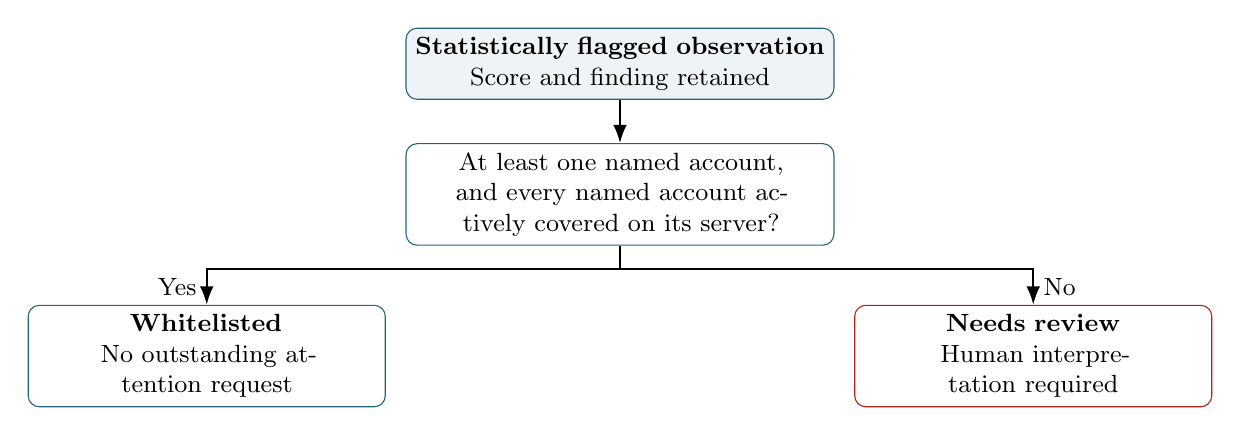
\begin{tikzpicture}[font=\small,>=Latex,
box/.style={draw=accent,rounded corners,align=center,text width=5.2cm,minimum height=0.85cm}]
\node[box,fill=pale] (finding) {\textbf{Statistically flagged observation}\\Score and finding retained};
\node[box,below=0.55cm of finding] (check) {At least one named account, and every named account actively covered on its server?};
\node[box,text width=4.3cm,below left=0.75cm and 0.25cm of check] (covered) {\textbf{Whitelisted}\\No outstanding attention request};
\node[box,text width=4.3cm,draw=reviewred,below right=0.75cm and 0.25cm of check] (open) {\textbf{Needs review}\\Human interpretation required};
\draw[->,thick] (finding) -- (check);
\draw[->,thick] (check.south) -- ++(0,-0.3) -| node[pos=0.75,left] {Yes} (covered.north);
\draw[->,thick] (check.south) -- ++(0,-0.3) -| node[pos=0.75,right] {No} (open.north);
\end{tikzpicture}
\caption{User whitelisting changes attention after scoring. For an unreviewed historical group, all its flagged observations must follow the covered branch before the whole group is overridden. Existing human reviews remain separate.}
\label{fig:whitelist-flow}
\end{figure}

IP whitelisting is not implemented. Phase 9's approved-automation addresses supply interpretive context to optional language-model triage and do not implement this override. The existing eight whitelist tests passed on 12 October 2026 using isolated temporary stores: password and validation checks, audit and retained removal records, expiry, matching, windows, partial groups, missing facts and uploads. They establish software behaviour, not attack-detection quality. Evidence: \nolinkurl{triage-console/service/whitelist.py} and \nolinkurl{triage-console/tests/test_whitelist.py}.

\subsubsection{Frozen Runtime and Evidence Availability}\label{sec:frozen-runtime}

The original \nolinkurl{data/} corpus has been purged from this workspace. The frozen runtime retains fitted preprocessing, detectors, model-zoo artifacts, map coordinates, group summaries and selected caches for inference on new supported uploads. It cannot recreate historical raw evidence or serve as a complete reproducible training dataset. Historical SQL, group-member lines and surrounding-event retrieval report the purge; retained new uploads supply their own excerpt context for Review.

The results below are historical recorded results, not new measurements on the purged corpus. Raw lines, accounts and addresses are omitted from the runtime package; separate console stores, retained uploads, reports and screenshots may still contain them. Historical whitelist matching requires exact retained review facts and fails closed when they are absent. See \nolinkurl{scripts/freeze_runtime.py} and \nolinkurl{triage-console/service/config.py}.

\subsubsection{Known-Pattern Rules (Sigma)}\label{sec:sigma-impl}

The statistical detectors rank what is rare; some attacks of concern are common and well described. The Sigma page therefore runs detection rules in the Sigma format, a vendor-neutral way of writing log detections \cite{ref28}, over logs that Phase 1 can read (\nolinkurl{triage-console/service/sigma.py}). A rule matches single events through named selections of field tests combined by its condition (\emph{and}, \emph{or}, \emph{not}, parentheses, \emph{1 of} and \emph{all of}), with the standard modifiers, wildcards and keyword lists. A correlation looks across events in a sliding window per group: at least $N$ matching events, at least $N$ distinct values of a field, or all the referenced rules within the window, optionally in order. Fields are Phase 1's names, with common Sigma and ECS names mapped to them, and a rule's log source selects the log type; a rule for a source the console does not read applies to nothing. Regular expressions run with a time limit per match, and rule files are read with a safe YAML loader.

Rules are kept in the console's store and run on demand on the same inputs as Analyze, or on a folder on the laptop: every file of its lowest folders, each told its log type by its first lines and its month by its folder names, the files of one log type and month checked together, one group in memory at a time. The enabled rules also run, as a fifth detector, over every Analyze input and upload and over the historical validation and test periods (\nolinkurl{sigma_review.py}): a hit flags every observation holding one of its lines, in every view, and Review lists any group holding such an observation whatever its lift, under the rule's title. The Dashboard counts these Sigma matches among the items waiting and lists them first. A hit whose events name only whitelisted accounts says so. Eight starter rules cover SSH password guessing, password spraying, user enumeration, a success after guessing, repeated \tok{su} failures, a stopped OSSEC agent, and firewall port scans and address sweeps; their thresholds are starting values awaiting operational confirmation. A rule is written in one of three ways: a form, the default, holding the fields most rules need and written as Sigma YAML, a count becoming a correlation, and read back without losing what it does not show (\nolinkurl{sigma_form.py}); a plain-English description from which the local model drafts a rule (\nolinkurl{sigma_ai.py}), its answer treated as untrusted text, read with the safe loader, checked by the engine, returned once with the engine's error and never saved by itself, a proof of concept tested against a stand-in model; or YAML. Every draft goes \emph{Draft}, \emph{Test}, \emph{Accept}: \emph{Accept} stays locked until the draft as it now stands has run over input, and the activity log records whether the accepted text was tested. Each rule shows who added it and when.

\subsection{Reports, Case History and Governance}\label{sec:reports}

Reports offer anomaly and malicious-activity templates with findings, raw-log evidence, tables, maps, timelines, commentary and method notes. Tables can be built by hand or from reviewed SQL; the local model can draft a query, but the analyst reviews and runs it. Offline ATT\&CK search suggests techniques, and accepting one is the analyst's decision. MITRE describes ATT\&CK as a knowledge base of adversary behaviour observed in the real world \cite{ref10}; a mapping names a behaviour, it does not prove malice.

Each case gets a number of the form \nolinkurl{IR-YYYY-NNNN}. Every save creates a new immutable version holding the document, its print evidence, the actor, the time and a SHA-256 digest, written in one transaction with the finding links and the audit entry. A save based on an older version is refused, so nobody overwrites a newer version unknowingly. Closing a case does not freeze it: reviewers can reopen and edit it, and each save adds a version.

Word, PDF and HTML exports use the evidence saved with the version, not current data or AI, so a version keeps its meaning after the analysis is updated. The digest shows whether content changed; it is not a digital signature, and typed sign-offs are not cryptographic.

\textbf{From Review.} A reviewed item has a \emph{Report} button that starts a new anomaly report about it: the title, the target particulars, the detection tiles and a finding card come from the item, and the item's saved notes become the analyst comments, exactly as typed, oldest first, each under its reviewer, time and label. Nothing is reworded and no language model is involved; the draft is then edited, saved and exported as any other report. An HTML export, beside Word and PDF, is the saved paper with its styles; it carries a content security policy that allows no script and no request, its pictures embedded.

\textbf{Example.} An analyst saves a new anomaly report; it receives the number \tok{IR-2026-0007} and becomes version 1, stored with the analyst's name, the time and a SHA-256 digest of its content. A colleague opens version 1 to add a timeline. Meanwhile the analyst adds a log-lines block and saves version 2. When the colleague saves, the console refuses, because their edit was based on version 1, and asks them to reload version 2 and reapply the timeline, which becomes version 3. A month later the AUTH models are retrained and some scores change; exporting version 2 to PDF still shows the evidence exactly as it was saved, because the export reads the saved copy rather than querying the data again.

The version register and source archives record application releases, not case history. Neither is yet a registry of approved rules, training datasets and deployed models; that needs a future governance process.

\subsection{Security of the Local Service}\label{sec:security}

The console holds sensitive logs, so its local service is built to be reachable only by the analyst's own browser page, and every place a person or a log can supply text is treated as untrusted input.

\textbf{Who can call it.} The service listens on \nolinkurl{127.0.0.1} only. A request must name this laptop as its host, which defeats DNS rebinding, and must not carry another site's origin. Every API request must also carry a header that only the console's own scripts add and must not be marked by the browser as coming from another site or the address bar; the service answers no cross-origin preflight, so another site's script cannot add the header. Changes are accepted only as JSON, which an ordinary web form cannot send. The page itself runs only its own scripts under a content security policy, loads nothing from elsewhere and cannot be framed, which prevents click-tricking from another page.

\textbf{Passwords.} An administrator password protects the activity log, the whitelist and the clearing of uploads; a separate SQL password protects queries. Both are kept as salted PBKDF2 hashes, each wrong guess costs a second, and checks are made one at a time, so parallel requests cannot share out that delay. SQL unlock tokens are random, kept in memory only and lapse after 30 minutes without a query. Both defaults are flagged in Settings until changed; the SQL default of four digits is a convenience, not a strong secret.

\textbf{Code injection.} Log lines, comments, notes, tile text and model output are always inserted as text, never as HTML, and documents pass a sanitiser. SQL runs only through three read-only layers (a text check, an engine-level read-only connection with an allow-list authoriser, and stores attached read-only), and queries the console writes itself use only checked values, with their comment lines kept on one line. Regular expressions in pattern and Sigma rules run with a time limit, and nested repeats are refused. A rule exported for Phase~1 is written as a string literal that reads back as the same text, so a rule cannot become code in the pipeline. Spreadsheet exports keep any cell that a spreadsheet would run as a formula as text. Links to ATT\&CK are made only for MITRE's own pages, and a tile can open only the console's own pages.

\textbf{Crafted files.} A workbook is a compressed archive of XML: parts that unpack beyond 256~MB are refused, cells claiming a column past Excel's last are ignored, and the text extracted is capped; the XML parser does not resolve external entities and limits entity expansion. Lines longer than a megabyte are cut when folders and archives are read. The language-model address must be an \nolinkurl{http} address on this laptop, and the model client follows no redirect.

\textbf{Residual risk.} Any program running on the laptop with the user's rights can still call the service; the design assumes a single-user analyst laptop with endpoint protection. These measures are checked by tests over real HTTP requests (\nolinkurl{tests/test_security.py}, \nolinkurl{tests/test_server_access.py}, \nolinkurl{tests/test_sql_lock.py}); they establish behaviour under test, not a penetration-tested deployment.

\subsection{Local AI and the Learning Feedback Loop}\label{sec:localai}

Optional triage by a local language model organises evidence and suggests a category: security relevant, operationally interesting, expected behaviour or insufficient context. Its output must be checked against the evidence. A full-report AI writer is deliberately deferred. This triage is a starting point for the planned context layer (requirement P5): it reads documented benign look-alikes and an approved-automation list, which is currently empty, but it is not connected to account directories, inventories, change records or calendars and it removes nothing.

The supervised-learning area has label preparation and TF-IDF/SecureBERT classifier scaffolding, but no trained malicious-versus-benign classifier based on independently labelled data. Exporting console labels for training is also unfinished. Handwritten or simulated triage examples are not ground-truth labels. Together with the frozen baselines and recorded reviews, this scaffolding is the foundation for the tertiary goal (requirement P7).

\textbf{Example.} For a flagged group of sessions in which one address tried forty invented user names on one host within ten minutes, the local model might suggest \emph{security relevant} because the pattern resembles password guessing, and the offline ATT\&CK search might rank the technique Brute Force: Password Guessing (T1110.001) first. The analyst checks the evidence before accepting either: if the address belongs to an internal vulnerability scanner scheduled for that night, the right label is \emph{expected behaviour}, and the mapping is not added. The model's suggestion and the analyst's decision are both kept, but only the analyst's label counts as a review.

Running locally keeps sensitive logs off external services, but the deployment's security still depends on access control, endpoint protection, backups, retention and administrators. The application is not a validated multi-user security platform or a replacement for a SIEM.

\clearpage
\section{Application User Guide and Screenshots}
\label{app:user-guide}

\label{sec:guide}

\textbf{Edition and evidence availability.} This guide describes the current workspace inspected on 26 October 2026. The screenshots predate the grouped menu, the redesigned and customisable Dashboard, the Sigma page and the SQL password; where a screen has changed, the text describes the current behaviour. The screenshots were captured on 9 October and may show the former branding, earlier layouts and historical evidence that is now unavailable. They illustrate the workflow rather than establish the current whitelist state. Section~\ref{sec:frozen-runtime} explains the retained inference runtime: new supported uploads still carry their own review evidence, while SQL, member-line and surrounding-event queries cannot recover the purged historical corpus.

This section describes, in broad strokes, what each part of the console is for and how an analyst uses it. The console runs on the analyst's laptop: the service listens on \nolinkurl{127.0.0.1:8765} and the pages open in a browser on the same machine. The screenshots were taken on 12 October 2026 at a width of 1,440 pixels in the light theme. Screens showing the historical data have log text, addresses and account names blurred; screens showing uploads and new formats use made-up lines whose addresses come from the range reserved for documentation (\nolinkurl{192.0.2.0/24}).

\subsection{Getting Around}

The sidebar holds a \emph{Simple}/\emph{Advanced} switch and the pages of the chosen mode. Simple mode has four pages (Check logs, Review, Reports and Settings) for people who need to check a file and record a judgement. Advanced mode has eleven, grouped in the order of an investigation: \emph{Overview} (Dashboard), \emph{Prepare} (Datasets, Patterns, Models), \emph{Detect} (Analyze, Sigma), \emph{Investigate} (Review, Data), \emph{Report} (Reports) and \emph{Console} (Documentation and Settings). The arrows at the foot of the menu shrink it to one icon per group; pointing at or clicking a group's icon opens its pages beside the menu, and a group of one page opens it directly. While a page waits for its data, one train circles its track in the middle of the screen. Pages that show one source have a \emph{Log type} selector at the top. The model picker at the top right chooses the local language model and shows, with a coloured dot, whether the local model service is running; the dot is red in these screenshots because the service was stopped. Long operations, such as a scan, a query or an analysis, show a short waiting animation with their progress; Settings chooses its style.

\subsection{Simple Mode: Check Logs}

\emph{Check logs} takes an analyst through four numbered steps: Upload, Analyze, Map and Review.

\textbf{Upload.} The analyst pastes lines or chooses a file: plain text, a CSV export or an Excel workbook. As soon as the lines arrive, the console detects the log type and the month and shows how much of the first 200 lines Phase 1 recognises (Figure~\ref{fig:simple-upload}). For a table, the raw-log column is offered as a dropdown, the month is taken from the time column and the server from a single-host column.

\screenshot{simple_upload.jpg}{0.98}{Simple mode, step 1: lines pasted, log type detected (AUTH), 100\% of the first lines recognised and the month filled in. Made-up lines.}{fig:simple-upload}

If fewer than 5\% of those lines are recognised, the step stops with \emph{Unknown log format} and offers \emph{Find patterns}, which opens the lines in the Patterns workbench (Figure~\ref{fig:simple-unknown}). The analysis is not run, so a result of nothing unusual cannot be misread as covering lines the parser could not read.

\screenshot{simple_unknown.jpg}{0.98}{Simple mode stopping at an unknown format: none of the first lines is recognised, so the console offers \emph{Find patterns} instead of an analysis. Made-up lines.}{fig:simple-unknown}

\textbf{Analyze.} \emph{Analyze} applies the saved preprocessing and models of the detected log type and returns a verdict, such as \emph{Unusual}, with the number of unusual findings, how rare the rarest one is and the server (Figure~\ref{fig:simple-verdict}). An active user exception can instead produce \emph{Whitelisted} when all relevant flagged findings are covered; their model scores remain unchanged. These counts describe the observations or retained findings used by the workflow, not a count of malicious log lines.

\screenshot{simple_verdict.jpg}{0.98}{Simple mode, step 2: the verdict for the uploaded lines. Made-up lines.}{fig:simple-verdict}

\textbf{Map.} \emph{See on the map} places the uploaded observations among the historical ones, using the saved embedding and nearest-neighbour placement, and lists the nearest groups with what is known about them: how many uploaded observations fall near them, how many are unusual, and whether the group is usually flagged (Figure~\ref{fig:simple-map}). The axes of a t-SNE or UMAP map carry no meaning of their own; nearby points behave alike.

\screenshot{simple_map.jpg}{0.98}{Simple mode, step 3: the uploaded observations (large red points) on the historical AUTH map, with the nearest groups. Made-up lines on the historical map.}{fig:simple-map}

\textbf{Review.} \emph{Send for review} keeps the upload as a review item. Reviewers then label it on the Review page; an upload can be cleared only with the activity-log password.

The retained upload includes its own excerpt context and can be inspected after the historical corpus purge. Use those uploaded lines for the current demonstration; the historical stores cannot supply purged neighbouring activity. Selected source lines have a \emph{this} marker and a tinted background; this is an observation-selection cue, not a maliciousness verdict. Sending to a named reviewer opens a mail draft and records assignment locally; it does not establish that an email has been delivered.

\subsection{Dashboard}

The Dashboard answers three questions in order: what needs a decision, what to open first, and how the work and the data stand (Figure~\ref{fig:dashboard} shows its earlier layout). Four headline cards come first: items waiting for review, those of them matching a Sigma rule (the card turns red while any wait), items labelled security relevant with the suspicious ones beside them, and the share reviewed with review decisions per day; each splits its figure by log type. \emph{Next to review} lists up to six waiting items, Sigma matches first and then each log type's queue in turn, and opens one in Review. \emph{Review progress} shows every item by its state per log type. \emph{Flagged} gives the share of test observations flagged in AUTH sessions and OSSEC episodes, per log type, and \emph{Detectors} shows which of the four mechanisms flagged them as a Venn diagram. \emph{Data} gives each log type's lines, months, event types and distinct messages, and the header shows the months the data spans; \emph{Model data} and \emph{Activity} follow at the foot. The page carries no explanatory text: each card's information icon explains it, and a table icon shows a chart as a table.

\textbf{Customising the Dashboard.} Settings $\rightarrow$ Dashboard shows the Dashboard itself, scaled down, as its editor. Cards are dragged into order, widened or narrowed from their right edge (3 to 12 of 12 columns), hidden into a tray and brought back. \emph{SQL table} adds a card holding the result of a read-only query of the analyst's own, with a title, a description behind its information icon and a height dragged from its bottom edge; the result is kept until the card's refresh button runs the query again, which asks for the SQL password. \emph{Tile} adds a small card, one column by one row to start, with an icon, a heading in one of three sizes, text, a colour, an alignment and optionally a console page that it opens; its width (1 to 12 columns) and height are dragged. \emph{Pack tightly} lets short cards fill the gaps beside tall ones. Nothing changes until the layout is saved; \emph{Discard} returns to the saved layout and \emph{Reset} to the standard one.

\screenshot{dashboard.jpg}{0.98}{The Dashboard over the historical data in its earlier layout, before the redesign described above: review workload, corpus size, the outlier share and review progress.}{fig:dashboard}

\subsection{Patterns: Onboarding a New Log Format}

Patterns is the workbench of Section~\ref{sec:patterns}, used when Phase 1 does not recognise a source. The analyst pastes lines, uploads a file or names a file, folder or archive on the laptop, and chooses a log type or leaves \emph{Detect}.

\textbf{Tables.} When the input is a CSV or Excel export, the console checks its first 100 rows and asks for two choices before scanning: the column that holds the raw log line, and the columns to keep. Each column is shown with its inferred type and its first five values (Figure~\ref{fig:patterns-table}). \emph{Scan} stays disabled until the table is well formed and a raw-log column is chosen.

\screenshot{patterns_table.jpg}{0.98}{Patterns, reading a CSV export: the table check, the raw-log column (1) and the columns to keep with their types and first values (2); the \emph{port} column is left out. Made-up lines.}{fig:patterns-table}

\textbf{Coverage.} A scan runs the first pass and shows coverage: the share of lines recognised, split into lines named by Phase 1 or by rules, lines whose prefix alone is recognised, and unknown lines; the passes so far; coverage over time, from the dates in the lines or the table's time column; and coverage per value of each kept field (Figure~\ref{fig:patterns-coverage}). A new log type is named and created here, and \emph{Run pass} re-reads the input with the rules saved so far.

\screenshot{patterns_coverage.jpg}{0.98}{Patterns after two passes over a made-up RADIUS export: 24.9\% of lines named by rules, the rest cut by a saved prefix; coverage per day; and coverage per host.}{fig:patterns-coverage}

\textbf{Shapes and lines.} The \emph{Shapes} card groups the lines not yet named into masked templates, under three tabs: candidate prefixes (line heads), messages and suffixes (line endings), each with its count of lines and a \emph{new} marker where it first appears late in the period (Figure~\ref{fig:patterns-lines}). The \emph{Lines} card lists the lines themselves, filtered to unknown, known or all lines and searchable, with the prefix, message and suffix of each line shaded in their own colours. Text selected in a line, or a shape's \(+\) button, sends examples to the regex builder.

\screenshot{patterns_lines.jpg}{0.98}{Patterns: message shapes with their line counts, and the lines with the saved prefix shaded. Made-up lines.}{fig:patterns-lines}

\textbf{Regex.} The builder proposes candidate regular expressions for the examples, each with the number of examples it matches and an estimate of the lines it would match in the whole input (Figure~\ref{fig:patterns-regex}). The analyst picks one, edits it if needed, names the event type and saves it. The examples below show live what the expression takes, with each named group's name above its value. Saved rules can be switched off, reordered, deleted and exported as JSON or as lines for Phase 1's rule list.

\screenshot{patterns_regex.jpg}{0.98}{Patterns: the regex builder with three candidates (Exact, Fields, Start), the chosen expression and event type, and the examples with their named groups. Made-up lines.}{fig:patterns-regex}

\subsection{Analyze}

Analyze is the advanced counterpart of \emph{Check logs} (Figure~\ref{fig:analyze}). The analyst pastes lines, uploads a file or names a file on the laptop; the log type, month and server can be set or left to detection, and example lines are available for each source. A progress line follows the analysis through parsing, classification, observations, features, models and the map. The result gives a verdict with the share of validation observations that are less unusual than the uploaded ones, the facts of the upload (log type, lines recognised, time span and servers) and one card per view with its flagged observations. When no log type recognises the lines, Analyze offers \emph{Find patterns}, as Simple mode does.

\screenshot{analyze.jpg}{0.98}{Analyze: four made-up AUTH lines, the processing steps, the verdict and the views.}{fig:analyze}

\subsection{Sigma: Known Attack Patterns}

Sigma runs detection rules written in the Sigma format over logs Phase 1 can read (Section~\ref{sec:sigma-impl}). The input is chosen as on Analyze: pasted lines, an uploaded file, or a file or folder on the laptop; a folder is read file by file from its lowest folders, each file's log type told from its first lines and its month from its folder names, and the files of one log type and month are checked together. \emph{Run} applies every rule that is on and lists the hits, the most serious first, each with its rule, level and the lines behind it; a hit whose accounts are all whitelisted says so. The rules are listed on the left, each with who added it and when, and a \emph{New} mark for a week. A rule is written on the right in a form (the default), from a plain-English description that the local model turns into a draft (a proof of concept), or as YAML, each with a live check of how the engine reads it. Under the editor, \emph{Draft}, \emph{Test} and \emph{Accept}: \emph{Test} runs the draft alone over the input, and \emph{Accept} opens only once the draft as it stands has been tested. Rules can be imported and exported as YAML files. No screenshot of this page is included in this edition.

\subsection{Models}

Models shows what was trained for the chosen log type and how it behaved on the test period (Figure~\ref{fig:models}). One card per view gives the test alerts out of the test observations and the alerts of each primary detector (robust deviation, Isolation Forest and novelty), with details on request; a view with too little data, such as AUTH daily behaviour, is marked as excluded from alerts. The model-zoo section below shows each view's ensemble for the full or selected features. \emph{Retrain} is locked here: training is started from Datasets by a signed-in administrator.

\screenshot{models.jpg}{0.98}{Models for AUTH: the views used for alerts, test-period alerts per view and detector, and the start of the model-zoo section.}{fig:models}

\subsection{Data: Message Types, Clusters and SQL}

Data explores the historical corpus of one log type through three tabs. Each begins with the timeline of the training, validation and test periods of every view.

\textbf{Message types} draws the year's lines as a flow from the log type through event categories to event types, each with its line count and its number of distinct messages once addresses, numbers and identifiers are blanked (Figure~\ref{fig:data-sankey}). A month range narrows the period, \emph{Equal width} and \emph{Height} change the drawing, and every type is also available as a table.

\screenshot{data_sankey.jpg}{0.98}{Data, message types: AUTH lines by category and event type, with line counts and distinct messages.}{fig:data-sankey}

\textbf{Clusters} draws a view's map of similar activity on request, with flagged observations in red, and lists its groups with their size and flagged count (Figure~\ref{fig:data-clusters}). Groups can be found by name, shown or hidden on the map, renamed and commented on; clicking a point opens its time, group, votes and original lines.

\screenshot{data_clusters.jpg}{0.98}{Data, clusters: the t-SNE map of AUTH individual lines and its groups.}{fig:data-clusters}

\textbf{SQL} runs read-only queries over the event stores \nolinkurl{auth.events}, \nolinkurl{ossec.events}, \nolinkurl{fw.pf_events} and \nolinkurl{fw.ipf_events} (Figure~\ref{fig:data-sql}). Example queries fill the editor, Ctrl+Space suggests table and column names, and a result can be downloaded as CSV or placed in a report table. Every query, including a refused one, is written to the activity log. The first query of a session asks for the SQL password (1234 until changed in Settings); after 30 minutes without a query it is asked again. A CSV download keeps any cell that a spreadsheet would read as a formula as text.

\screenshot{data_sql.jpg}{0.98}{Data, SQL: an example query on failed SSH logins, with the available tables.}{fig:data-sql}

\subsection{Review}

The current queue also distinguishes \emph{Whitelisted} groups from findings needing attention. A historical group is fully overridden only when every flagged observation is covered by the active user list; partial coverage leaves the group open. The whitelist does not replace a human review label. After the purge, profiles and filters depend on retained facts, while original historical lines and their surrounding context are unavailable; retained uploads supply their own excerpt context.

Review is where flagged groups receive a human judgement (Figure~\ref{fig:review}). Filters at the top match server, account, program and address against the original events: values of one field are alternatives, and different fields must hold on the same event. The left column lists the groups needing review, or those already reviewed, for the chosen view and period, with their servers, size and dates. Opening a group shows how many unusual observations it holds, when they were seen and their servers, accounts, source addresses and programs with their shares. The analyst chooses one of five labels (security relevant, suspicious, operationally interesting, expected behaviour or insufficient evidence) and may add a note. Below, the group's most unusual events are listed by rarity; opening one shows its lines and the logs around it on the same server. \emph{Uploads} switches to items sent from Simple mode. A reviewed item has a \emph{Report} button, which starts an anomaly report about it with its saved notes as the analyst comments (Section~\ref{sec:reports}).

\screenshot{review.jpg}{0.98}{Review: AUTH session groups awaiting review and one group's profile, labels and rarest events. Account names and addresses are blurred.}{fig:review}

\subsection{Reports}

Reports assembles an investigation report on a paper-like page (Figure~\ref{fig:reports}). The toolbar chooses the template (anomaly or malicious activity), opens saved reports and their versions, previews, exports to PDF, Word or HTML, and saves a new version. Blocks on the left (text, target, finding, log lines, table, metric, ATT\&CK technique, timeline, cluster map, AI draft and signature) and sections are added to the page; reviewed findings on the right are dragged in as evidence. The report number is assigned on the first save, and each save keeps an immutable version (Section~\ref{sec:reports}).

\screenshot{reports.jpg}{0.98}{Reports: a new anomaly report with the block palette and the list of reviewed findings, whose titles are blurred.}{fig:reports}

\subsection{Datasets}

Datasets lists the datasets the pipeline knows, with their log type, source and last training (Figure~\ref{fig:datasets}). Adding a dataset (a folder of monthly archives), importing its archives and training from a chosen phase change the data everyone relies on, so they require an administrator signed in through single sign-on; until it is configured, the page is read-only and says so.

\screenshot{datasets.jpg}{0.98}{Datasets without single sign-on configured: the dataset list and the start of the form for adding one, both read-only.}{fig:datasets}

Below the datasets, \emph{Unapproved log types} lists the log types created in Patterns, with their number of rules, last scan and table layout (Figure~\ref{fig:datasets-unapproved}). Any user can delete one with two clicks; deletion removes only the workbench's own records and is written to the activity log.

\screenshot{datasets_unapproved.jpg}{0.98}{Datasets: an unapproved log type created in Patterns, with its delete button. Made-up log type.}{fig:datasets-unapproved}

\subsection{Documentation}

Documentation presents the pipeline as a transit line: each phase is a station, and the sub-phases branch off at interchanges (Figure~\ref{fig:docs}). Choosing a station shows what the phase does and produces, links to its notes and steps to the neighbouring stations. Below, the user guides, the requirements and design documents and the pipeline's own notes open inside the console.

\screenshot{docs.jpg}{0.98}{Documentation: the pipeline line with the Classify station open.}{fig:docs}

\subsection{Whitelisted Users: Adding and Removing an Exception}\label{sec:whitelist-guide}

In Advanced mode, open Settings and find \emph{Whitelisted users}. This is the account-level postprocessing feature of Section~\ref{sec:whitelist}; it applies to the findings used by Analyze, Simple mode and Review without changing their model scores.

\begin{enumerate}
\item Enter one exact \emph{Account}. Account names are case-sensitive. Enter a \emph{Server} to restrict the exception, or leave it blank for all servers.
\item Enter a \emph{Reason} explaining the approval. Optionally choose an \emph{Until} date: the entry applies through that day and expires afterwards. Blank means no date limit.
\item Enter the local administrator \emph{Password} and choose \emph{Add}. The list records scope, reason, expiry, author and time; the change is written to the activity log.
\item Reopen a retained upload or run the supported check again. Covered findings show \emph{Whitelisted}; any remaining uncovered findings still request attention. Do not infer that the model's score changed.
\item To withdraw approval, choose the entry's removal control, supply the password and confirm. The record is retained with removal author and time. Expiry or removal restores attention for still-unreviewed findings when the active list is evaluated again.
\end{enumerate}

\begin{table}[H]
\centering\small
\begin{tabular}{p{0.51\linewidth}p{0.40\linewidth}}
\toprule
\textbf{Finding, with an active \tok{backup}/\tok{host-a} entry} & \textbf{Coverage outcome} \\
\midrule
Only \tok{backup} named, on \tok{host-a} & Covered, including failed logins \\
\tok{backup} named on another server & Not covered by this scoped entry \\
Both \tok{backup} and unapproved \tok{root} named & Not covered: every named account must match \\
No account named anywhere in the observation & Not covered \\
\tok{backup} plus lines with no account, on \tok{host-a} & Covered: unnamed lines do not block a named match \\
\bottomrule
\end{tabular}
\caption{Practical matching examples. The entry must be active, and other applicable entries can affect the outcome. A covered observation remains statistically flagged and retained.}
\label{tab:whitelist-matching}
\end{table}

The exception is not restricted to a specific approved command or successful-login pattern. For that reason, use a justified server scope and expiry. This feature accepts accounts, not IP addresses; Phase 9's approved-automation address context remains separate. For a historical group whose exact account facts were not retained, the application leaves the finding uncovered.

\subsection{Settings}

Settings includes \emph{Whitelisted users}, with account, server scope, reason, expiry and password-protected additions and removals. Existing screenshots predate this feature; the current behaviour is described above. Settings holds the console's local configuration (Figure~\ref{fig:settings}): language, console mode, theme, font, text size and the waiting animations, with previews; the local language model, the address of the local model service, and the name recorded with comments and reviews. The activity log at the bottom lists every recorded change with its time, actor, action, object and detail. Clearing it requires the activity-log password, and the page warns while the default password is still in use. Settings also holds the Dashboard editor described under Dashboard, and two passwords: the administrator password for the activity log and the whitelist, and the SQL password for queries; a warning shows while either default is in use. \emph{Review} holds the filter time limit, 120 seconds unless changed: a Review filter that runs longer, including the one-time preparation of its facts, is stopped with a message.

\screenshot{settings.jpg}{0.98}{Settings: appearance, the local language model, and the activity log showing the pattern rules saved for the made-up RADIUS export.}{fig:settings}

\clearpage
\section{Detailed Historical Results and Acceptance Programme}
\label{app:results}

\subsection{Dataset and Scope of the Evidence}

The following figures come from the saved project outputs and their documentation, principally the September source reprocessing and the 8 October sequence runs. They describe one historical environment, not a multi-site benchmark.


\begingroup
\small
\begin{longtable}{>{\RaggedRight\arraybackslash}p{\dimexpr 0.12\linewidth-2\tabcolsep\relax}>{\RaggedRight\arraybackslash}p{\dimexpr 0.17\linewidth-2\tabcolsep\relax}>{\RaggedRight\arraybackslash}p{\dimexpr 0.16\linewidth-2\tabcolsep\relax}>{\RaggedRight\arraybackslash}p{\dimexpr 0.55\linewidth-2\tabcolsep\relax}}
\caption{Current historical log corpus}\label{tab:5}\\
\toprule
\rowcolor{pale} \textbf{Source} & \textbf{Raw lines in the current corpus} & \textbf{Observed event types} & \textbf{Interpretation} \\
\midrule
\endfirsthead
\multicolumn{4}{l}{\small\itshape Table \thetable{} --- continued}\\
\toprule
\rowcolor{pale} \textbf{Source} & \textbf{Raw lines in the current corpus} & \textbf{Observed event types} & \textbf{Interpretation} \\
\midrule
\endhead
\midrule
\multicolumn{4}{r}{\footnotesize Continued on the next page}\\
\endfoot
\bottomrule
\endlastfoot
AUTH & 26,091,162 & 61 & Authentication-related logs across the study year; 3,149 unrecognised lines, approximately 0.012\%. \\[3pt]
OSSEC & 115,288 & 46 & Agent operational messages; primarily connection and service behaviour. \\[3pt]
PF & 3,955 & 3 & Includes 3,415 packet records on 41 active days and 540 batch-script lines, rather than 3,955 network events. \\[3pt]
IPFilter & 52,231 & 2 & All activity occurs in November 2025; the other eleven monthly files are empty. About 99.98\% concerns port 9711. \\[3pt]
\end{longtable}
\endgroup


Source: \projectref{current corpus description}{README.md}, section ``A short security primer: the log sources''. The AUTH sequence stream accepts 26,085,863 timestamped events. This is a different denominator from raw lines; the difference should not be equated solely with unrecognised-message counts.

The corpus is heavily dominated by routine activity. Sparse firewall activity and highly repetitive authentication traffic justify source-specific methods. Neither sparsity nor repetition establishes that the remaining unusual events are malicious.

\subsection{Sequence Reconstruction and Learned Routines}\label{sec:routines-results}


\begingroup
\small
\begin{longtable}{>{\RaggedRight\arraybackslash}p{\dimexpr 0.52\linewidth-2\tabcolsep\relax}>{\RaggedRight\arraybackslash}p{\dimexpr 0.24\linewidth-2\tabcolsep\relax}>{\RaggedRight\arraybackslash}p{\dimexpr 0.24\linewidth-2\tabcolsep\relax}}
\caption{Sequence reconstruction and routine-mining results}\label{tab:6}\\
\toprule
\rowcolor{pale} \textbf{Recorded measure} & \textbf{AUTH sessions} & \textbf{OSSEC episodes} \\
\midrule
\endfirsthead
\multicolumn{3}{l}{\small\itshape Table \thetable{} --- continued}\\
\toprule
\rowcolor{pale} \textbf{Recorded measure} & \textbf{AUTH sessions} & \textbf{OSSEC episodes} \\
\midrule
\endhead
\midrule
\multicolumn{3}{r}{\footnotesize Continued on the next page}\\
\endfoot
\bottomrule
\endlastfoot
Events accepted into the sequence stream & 26,085,863 & 115,288 \\[3pt]
Observations across all partitions & 9,475,862 & 29,447 \\[3pt]
Distinct collapsed sequences across all partitions & 306 & 77 \\[3pt]
Cross-file copies merged & 290,396 & 4,692 \\[3pt]
Uncertain transitions recorded & 4,897 & 0 \\[3pt]
Training observations used for routine fitting & 6,632,522 & 20,608 \\[3pt]
Distinct sequences in routine fitting & 285 & 75 \\[3pt]
Routine catalogue rows, across scopes and summary types & 409 & 312 \\[3pt]
High-confidence rule rows & 53 & 81 \\[3pt]
\end{longtable}
\endgroup


Sources: AUTH \projectref{stream summary}{data/phase4f_sequences/auth/streams/summary.json} and \projectref{routine summary}{data/phase4f_sequences/auth/routines/summary.json}; OSSEC \projectref{stream summary}{data/phase4f_sequences/ossec/streams/summary.json} and \projectref{routine summary}{data/phase4f_sequences/ossec/routines/summary.json}.

The stream summaries record successful agreement with Phase 2 observation counts and Phase 3 split assignments. This supports integration correctness for the recorded run; it does not independently establish that every heuristic session boundary is semantically correct.

The main AUTH routine is:

\nolinkurl{SSH_LOGIN_SUCCESS}\allowbreak\,\ensuremath{\rightarrow}\,\allowbreak \nolinkurl{SSH_DISCONNECT_RECEIVED}\allowbreak\,\ensuremath{\rightarrow}\,\allowbreak \nolinkurl{SSH_USER_DISCONNECTED}

It accounts for approximately 82.3\% of the routine-fitting observations. A lone \nolinkurl{SSH_CONNECTION_CLOSED} contributes approximately 11.1\%, and a lone \nolinkurl{SSH_LOGIN_SUCCESS} approximately 4.6\%. Together, these three sequences account for about 98\% of that training population. Weighted compression therefore reduces millions of observations to hundreds of distinct sequences without discarding their support counts.

One learned rule links \nolinkurl{SSH_DISCONNECT_RECEIVED} to a later \nolinkurl{SSH_USER_DISCONNECTED} with 100\% observed confidence over 5,493,782 training sessions. An OSSEC rootcheck-start-to-end rule on one host has approximately 99.5\% confidence over 204 antecedent-bearing episodes. These are useful descriptions of recorded routines, not guarantees that future missing steps indicate compromise. Source: \projectref{sequence findings guide}{pipeline/phase4f_sequences/GUIDE.md}.

\subsection{Held-Out Sequence Alerts}\label{sec:seq-alerts}


\begingroup
\small
\begin{longtable}{>{\RaggedRight\arraybackslash}p{\dimexpr 0.52\linewidth-2\tabcolsep\relax}>{\RaggedRight\arraybackslash}p{\dimexpr 0.24\linewidth-2\tabcolsep\relax}>{\RaggedRight\arraybackslash}p{\dimexpr 0.24\linewidth-2\tabcolsep\relax}}
\caption{Held-out sequence scoring and alerts}\label{tab:7}\\
\toprule
\rowcolor{pale} \textbf{Measure} & \textbf{AUTH} & \textbf{OSSEC} \\
\midrule
\endfirsthead
\multicolumn{3}{l}{\small\itshape Table \thetable{} --- continued}\\
\toprule
\rowcolor{pale} \textbf{Measure} & \textbf{AUTH} & \textbf{OSSEC} \\
\midrule
\endhead
\midrule
\multicolumn{3}{r}{\footnotesize Continued on the next page}\\
\endfoot
\bottomrule
\endlastfoot
Validation observations & 1,420,844 & 4,415 \\[3pt]
Test observations & 1,421,114 & 4,417 \\[3pt]
Final score threshold, approximately & 11.5633 & 8.8097 \\[3pt]
Validation alerts at the final threshold & 543 & 19 \\[3pt]
Test alerts & 608 & 19 \\[3pt]
Test alert fraction & 0.0428\% & 0.4302\% \\[3pt]
\end{longtable}
\endgroup


Sources: AUTH \projectref{scoring summary}{data/phase4_detection/auth/sequences/authentication_sessions/summary.json} and OSSEC \projectref{scoring summary}{data/phase4_detection/ossec/sequences/episodes/summary.json}. The thresholds are surprise scores with a small tie-breaking term, not attack probabilities.

For AUTH, the validation-budget threshold determines the final boundary; for OSSEC, the training-quantile floor is higher and determines it. This prevents the OSSEC detector from filling its available validation budget with relatively ordinary transitions.

The AUTH findings include permission problems affecting \nolinkurl{authorized_keys}, invalid-user activity, session endings newly observed on particular hosts, and service restarts. The local qualitative analysis also identifies 244 alerts involving a lone \nolinkurl{SSH_SUBSYSTEM_NOT_FOUND} message on busy servers. These events were not necessarily new; a low relative frequency on a very busy host can still produce high surprise. This is an actionable calibration issue, not evidence of 244 attacks.

The nineteen OSSEC test alerts concentrate in two operational windows: a host's approximately 02:00 activity on 17 June and repeated agent restarts on another host on 13 July. They are investigation leads. The available evidence does not establish two confirmed cybersecurity incidents. These interpretations are based on the \projectref{recorded sequence investigation}{pipeline/phase4f_sequences/GUIDE.md}, whose informal descriptions require the qualifications above.

\subsection{Complementarity, Alert Concentration and Model Diversity}\label{sec:complementarity}

The Dashboard's overlap artifact combines four detector mechanisms over the AUTH-session and OSSEC-episode test views:


\begingroup
\small
\begin{longtable}{>{\RaggedRight\arraybackslash}p{\dimexpr 0.44\linewidth-2\tabcolsep\relax}>{\RaggedRight\arraybackslash}p{\dimexpr 0.28\linewidth-2\tabcolsep\relax}>{\RaggedRight\arraybackslash}p{\dimexpr 0.28\linewidth-2\tabcolsep\relax}}
\caption{Detector alert counts and unions in the two test views}\label{tab:8}\\
\toprule
\rowcolor{pale} \textbf{Detector or union} & \textbf{AUTH, 1,421,114 observations} & \textbf{OSSEC, 4,417 observations} \\
\midrule
\endfirsthead
\multicolumn{3}{l}{\small\itshape Table \thetable{} --- continued}\\
\toprule
\rowcolor{pale} \textbf{Detector or union} & \textbf{AUTH, 1,421,114 observations} & \textbf{OSSEC, 4,417 observations} \\
\midrule
\endhead
\midrule
\multicolumn{3}{r}{\footnotesize Continued on the next page}\\
\endfoot
\bottomrule
\endlastfoot
Isolation Forest & 370 & 367 \\[3pt]
Model-zoo consensus union & 5,653 & 6 \\[3pt]
Novelty & 1,202 & 209 \\[3pt]
Sequence & 608 & 19 \\[3pt]
At least one of these mechanisms & 6,287 & 383 \\[3pt]
\end{longtable}
\endgroup


Source: \projectref{saved overlap artifact}{triage-console/var/cache/outliers.json}, interpreted using \projectref{the overlap service}{triage-console/service/outliers.py}. Model-zoo counts here unite the full-feature and selected-feature \textbf{consensus} outputs. They are not the counts from the separate ensemble-score threshold.

Across these two test views, 6,670 of 1,425,531 observations are flagged, approximately \textbf{0.47\%}. This demonstrates selective prioritisation over these particular observations. It does not establish 99.53\% benign traffic, equivalent analyst-time savings or coverage of all raw lines and all observation views.

Of the 608 AUTH sequence alerts, 192 are not flagged by the other three mechanisms. The sequence detector overlaps model-zoo consensus on 416 observations and novelty on 56, with no Isolation Forest overlap in this view. These overlap counts are not mutually exclusive. The nineteen OSSEC sequence alerts all overlap novelty; six also overlap Isolation Forest. Sequence analysis therefore contributes complementary candidates in AUTH and additional explanation in OSSEC, rather than demonstrating uniform incremental attack recall across sources.

Alert profiling also reveals detector concentration. All 370 AUTH-session Isolation Forest alerts occur on the \nolinkurl{mm} host family; approximately 98.7\% contain \nolinkurl{SSH_DEPRECATED_OPTION}. The model-zoo alerts likewise concentrate on that family. These findings make a baseline problem visible and reviewable. They do not prove that every such alert should be suppressed. Source: \projectref{AUTH alert-profile artifacts}{data/phase4f_sequences/auth/alert_profile/summary.json} and \projectref{their interpretation}{pipeline/phase4f_sequences/GUIDE.md}.

The original draft's statement that all selected ensembles contain two models is no longer accurate. The current AUTH selected-feature five-minute ensemble contains ten families, while several other ensembles retain two. AUTH-session feature selection reduces 573 full features to 68 selected features; this is a representation change, not proof of higher security accuracy. Sources: \projectref{AUTH model-zoo results}{data/phase4_detection/auth/model_zoo/model_zoo_summary.csv} and \projectref{OSSEC model-zoo results}{data/phase4_detection/ossec/model_zoo/model_zoo_summary.csv}.

\subsection{Pattern-Discovery Throughput and Verification}

No workbench rule has yet been adopted into Phase 1, so this paper reports no change in the study corpus's coverage. The study corpus is already well covered for AUTH (3,149 unrecognised lines, about 0.012\%); the workbench's expected value lies in new sources and future format drift.

Development measurements recorded on 12 October 2026 on the project laptop describe throughput. For one month of AUTH logs from one host (1,059,233 lines), the first pass took about 21 seconds, mostly for Phase 1 classification of every line, and the next pass about 3 seconds, because Phase 1 results are kept while the input is unchanged. Read as an unknown log type, so that every line is masked and grouped, the same file took about 21 seconds for the first pass and 15 seconds for the next. These are single measurements, not benchmarks.

Twenty-eight automated tests cover shape masking and merging, refused patterns, rule suggestion, a full cycle from unknown to known lines on synthetic data, drift markers, the unknown-format check, deletion of unapproved log types, and tabular reading, including Excel workbooks and malformed tables. As with the other software tests, they verify implementation behaviour, not the quality of the rules an analyst writes. Sources: \projectref{pattern tests}{triage-console/tests/test_patterns.py} and \projectref{table tests}{triage-console/tests/test_tabular.py}.

\subsection{What Has Been Demonstrated Against the Problem Statement}


\begingroup
\small
\begin{longtable}{>{\RaggedRight\arraybackslash}p{\dimexpr 0.23\linewidth-2\tabcolsep\relax}>{\RaggedRight\arraybackslash}p{\dimexpr 0.39\linewidth-2\tabcolsep\relax}>{\RaggedRight\arraybackslash}p{\dimexpr 0.38\linewidth-2\tabcolsep\relax}}
\caption{Evidence against the problem-statement requirements}\label{tab:9}\\
\toprule
\rowcolor{pale} \textbf{Requirement} & \textbf{Evidence in the current application} & \textbf{Remaining qualification} \\
\midrule
\endfirsthead
\multicolumn{3}{l}{\small\itshape Table \thetable{} --- continued}\\
\toprule
\rowcolor{pale} \textbf{Requirement} & \textbf{Evidence in the current application} & \textbf{Remaining qualification} \\
\midrule
\endhead
\midrule
\multicolumn{3}{r}{\footnotesize Continued on the next page}\\
\endfoot
\bottomrule
\endlastfoot
P1: make heterogeneous logs usable & Source-specific parsing, several observation scales, retained lineage and processing of more than 26 million AUTH lines; a workbench that measures how much of a new or changed format is recognised and helps write parsing rules, including for CSV and Excel exports. & Parser coverage and observation boundaries need continued validation; OSSEC and firewall sources have limited semantic coverage; workbench rules reach the pipeline only through a manual change to Phase 1. \\[3pt]
P2: surface early signs & Multiple anomaly models, token novelty, whole-sequence summaries, host-conditioned transition scores, and presence and silence checks; in the AUTH test view, 192 of 608 sequence candidates were not flagged by the other three Dashboard mechanisms. & Unusual is not malicious. Whether flagged observations precede incidents, and by how long, has not been measured; quiet attacks that resemble ordinary activity may not be ranked. \\[3pt]
P3: rely less on static rules & Baselines, thresholds and frequent subsequences learned from unlabelled logs, with no attack rule written in advance; re-runnable pipelines, saved model artifacts, a source-version register and format-drift indicators (coverage over time, new shapes, quiet rules) let them be re-learned as systems change. & Normality is descriptive, not a security policy. Known attack-sequence templates, injected-attack evaluation, an approved rule registry, deployment integration, rollback and continuous effectiveness monitoring need further work. \\[3pt]
P4: account for recorded cases & Audited user whitelist applied after scoring, with exact account, server scope, optional expiry, required reason and administrator password; covered findings stay scored and retained; eight whitelist tests passed. & Accounts only, not addresses; an entry also covers failed logins naming that account, so scope and expiry need review; historical coverage fails closed where account facts were not retained. \\[3pt]
P5: add organisational context & Optional Phase 9 local-model triage with documented benign look-alikes and an approved-automation list; reviewers add context by hand. & No rule-based or agentic layer is connected to account directories, inventories, change records or calendars; the approved-automation list is empty; nothing is filtered automatically. \\[3pt]
P6: make alerts manageable and explainable & Validation calibration, overlap analysis, attribute profiles, original evidence and grouped review. & No measured analyst workload reduction or attack recall; some detectors are dominated by particular host behaviours. \\[3pt]
P7: retain decisions and labels for a classifier & Saved reviews in five dispositions, evidence-linked reports, immutable report versions, Word/PDF exports, frozen fitted baselines and Phase 8 label-preparation and classifier scaffolding. & Review quality depends on analyst judgement; label export to training is unfinished and no malicious/benign classifier has been trained or validated. \\[3pt]
P8: control evidence handling & Local execution, read-only analytical access, optional local AI and saved export evidence. & Enterprise identity, access, retention, backup and operational assurance must be validated for the intended deployment. \\[3pt]
P9: discover rules (added benefit) & 53 AUTH and 81 OSSEC sequential rules with at least 95\% confidence and frequent routines mined from training (Appendix~\ref{app:routines}); FP-growth alert profiles; each sequence finding names its unusual transition. & No mined rule has been reviewed, replayed or adopted; tracing findings back to chains before real incidents needs labelled incidents; non-intuitive candidates need extra justification and may reflect logging artefacts. \\[3pt]
\end{longtable}
\endgroup


This evidence supports use as an analyst-assisted early-warning and analysis workbench. It does not yet support a claim of warning before real incidents, automatic removal of false positives, malicious/benign classification or presenting the application as a complete unattended monitoring service.

\subsection{Limitations and the Validation Needed for Operational Acceptance}

The most important missing evidence is an independently reviewed set of malicious and benign observations. Without it, the project cannot establish attack precision, attack recall, false-negative rate or the superiority of one model for cybersecurity detection. A reported 100\% proxy \nolinkurl{detection_rate} does not resolve this limitation.

Other limitations include baseline contamination by unknown malicious activity, missing maintenance labels, concept drift, token-hash collisions, heuristic session boundaries, uncertain ordering and limited coverage of long-range attack sequences. Maps and cluster assignment tests assess representation and grouping behaviour, not maliciousness. Software tests establish implementation properties under their test conditions; they do not establish detection efficacy.

Pattern discovery adds its own limitations. Masking and merging can join distinct events or split variants of one event; suggested expressions generalise from the chosen examples and can be too broad or too narrow; coverage estimates while a rule is being written come from a sample; and drift markers depend on dates being present and on a fixed quarter-of-range convention. Recognising a line also says nothing about whether its event type is security-relevant.

An operational acceptance programme should therefore evaluate the following, with targets agreed before examining the final evaluation set:


\begingroup
\small
\begin{longtable}{>{\RaggedRight\arraybackslash}p{\dimexpr 0.25\linewidth-2\tabcolsep\relax}>{\RaggedRight\arraybackslash}p{\dimexpr 0.75\linewidth-2\tabcolsep\relax}}
\caption{Proposed operational acceptance programme}\label{tab:10}\\
\toprule
\rowcolor{pale} \textbf{Evaluation} & \textbf{Method and measure} \\
\midrule
\endfirsthead
\multicolumn{2}{l}{\small\itshape Table \thetable{} --- continued}\\
\toprule
\rowcolor{pale} \textbf{Evaluation} & \textbf{Method and measure} \\
\midrule
\endhead
\midrule
\multicolumn{2}{r}{\footnotesize Continued on the next page}\\
\endfoot
\bottomrule
\endlastfoot
Attack and benign ground truth & Independently adjudicate a temporally held-out sample, including flagged and unflagged observations. Use controlled attack exercises where appropriate; distinguish simulated coverage from real-world prevalence. \\[3pt]
Detection quality & Measure precision \(TP/(TP+FP)\), recall \(TP/(TP+FN)\), false alerts per host-day and detection delay, with uncertainty estimates and explicit units of counting. \\[3pt]
Lead time & For incidents and significant operational problems in the evaluation period, record whether related observations were flagged beforehand and how long before; report the share of flagged observations that preceded nothing of concern. \\[3pt]
Incremental benefit & Compare existing operational rules, numerical detectors and sequence detection on the same labelled periods and comparable review budgets. \\[3pt]
Recorded cases & Exercise whitelist scope, expiry and removal; review active entries on a fixed schedule; check whether covered accounts appear in findings later judged relevant. \\[3pt]
Context layer & Connect rule-based or agentic filtering to account, asset, change and maintenance sources; record each removal with its reason; measure the share of findings removed and audit a sample of removed findings for relevant activity. \\[3pt]
Classifier readiness & Measure agreement between reviewers, label coverage per source and view, and the performance of a classifier evaluated on a period later than its training labels. \\[3pt]
Data quality and negative controls & Test collection gaps, rotated duplicates, clock ties, maintenance, partial uploads and benign behavioural changes. \\[3pt]
Parsing coverage & For each new source, record coverage per pass and per source type, replay adopted rules on held-out months, and review a sample of newly named lines for misclassification. \\[3pt]
Operational efficiency & Measure review minutes, duplicate findings, time from discovery to an approved rule, and maintenance effort against the current process. \\[3pt]
Hypothesis resolution & For each group in the register (Appendix~\ref{app:hypotheses}), record the hypothesis that survived, the test that could have refuted it, and the resulting label or whitelist entry. Report the share of flagged groups resolved, the time per group, agreement between two reviewers on a sample, and any whitelisted account later involved in a relevant finding. \\[3pt]
Rule discovery & Replay mined candidate rules on held-out months, including maintenance; record how many survive review and approval, their alert volume, and whether non-obvious candidates find relevant activity that existing rules miss. \\[3pt]
Governance and deployment & Demonstrate ownership, documented logic, replay tests, approval, deployment, monitoring and rollback for a candidate rule. \\[3pt]
Security and recoverability & Validate identity integration, least-privilege access, retention, backup restoration and audit evidence in the intended environment. \\[3pt]
\end{longtable}
\endgroup


For a mined routine to become an operational detection rule, an analyst must add the meaning absent from frequency alone: protected asset and account scope, required telemetry, timing constraints, exceptions, severity, owner and expected response. Historical replay should include known benign maintenance and labelled attack scenarios. A candidate that is not intuitive to a person deserves the same treatment and more evidence, not less: its value is that nobody would have written it, and its risk is that nobody can easily explain it. Approval and integration into the organisation's monitoring platform would then complete a lifecycle that the present workbench only partially implements.

\subsection{Interpretation of the Historical Findings}

Project DAD (Data Anomaly Detection) Console demonstrates a practical step from reacting to incidents towards discovering early signs of them. It combines source-specific evidence preparation, complementary anomaly models learned from unlabelled logs, sequential behaviour analysis and an application for investigation and versioned reporting. Its strongest contribution is the connection between a statistical finding, the original log evidence and a recorded analyst judgement.

The sequential feature makes this contribution concrete. Millions of AUTH sessions compress into a small set of common event-type sequences; learned routines describe expected order, while host-conditioned transition scores identify deviations with explicit explanations. In the recorded AUTH test view, sequence scoring adds 192 candidate observations beyond the other three Dashboard mechanisms, without a rule written for any of them. This demonstrates complementary prioritisation, while leaving the security significance of those observations to validation and review.

The application can therefore support proactive review now: analysts can inspect rare behaviour, challenge detector assumptions, investigate triggers, record accepted cases as audited exceptions and retain their reasoning. When a new source arrives, they can also measure what the parser recognises and draft the missing parsing rules, although adopting those rules into the pipeline remains a manual, reviewed step. The mined routines and sequential rules offer a further source of detection logic, candidates a person may not have thought to write, once an analyst has reviewed and replayed them. Achieving the full problem statement requires a context layer that removes false positives using organisational knowledge, a classifier trained on quality-controlled labels, a governed production-rule lifecycle, and evidence of detection quality and lead time on independently assessed data. The evidence supports a staged pilot, not a claim that statistical analytics alone can anticipate incidents.

\clearpage
\section{Application Version History}
\label{app:versions}

The application's releases are recorded in the project's version register (\nolinkurl{VERSIONS.md}); each numbered release also has an immutable source archive with a SHA-256 manifest. Unreleased changes are dated entries that have not yet been given a version number or an archive.

\begingroup
\small
\begin{longtable}{>{\RaggedRight\arraybackslash}p{\dimexpr 0.15\linewidth-2\tabcolsep\relax}>{\RaggedRight\arraybackslash}p{\dimexpr 0.14\linewidth-2\tabcolsep\relax}>{\RaggedRight\arraybackslash}p{\dimexpr 0.71\linewidth-2\tabcolsep\relax}}
\caption{Application version history}\label{tab:versions}\\
\toprule
\rowcolor{pale} \textbf{Version} & \textbf{Date} & \textbf{Main changes} \\
\midrule
\endfirsthead
\multicolumn{3}{l}{\small\itshape Table \thetable{} --- continued}\\
\toprule
\rowcolor{pale} \textbf{Version} & \textbf{Date} & \textbf{Main changes} \\
\midrule
\endhead
\midrule
\multicolumn{3}{r}{\footnotesize Continued on the next page}\\
\endfoot
\bottomrule
\endlastfoot
0.1.0 & Inherited baseline & The console as it stood before the version register began; its web package identified itself as 0.1.0. No release archive was captured, so this version cannot be reproduced exactly. \\[3pt]
0.2.0 & 7 Oct 2026 & Reports and Review completion: case numbers of the form \nolinkurl{IR-YYYY-NNNN}, immutable report versions with actor, time and digest, conflict checks, Word and PDF export from saved evidence, target maps, timelines and anomaly and malicious-activity templates. Exact Review filters on server, account, program and address; password-protected clearing of uploads. A version controller for source archives. 84 unit tests. \\[3pt]
Unreleased & 8 Oct 2026 & Sequential pattern mining (Phase 4f): complete event streams for AUTH sessions and OSSEC episodes, weighted PrefixSpan routines, sequential rules, the transition-surprise detector and FP-growth alert profiles. A Dashboard Outliers card with a four-mechanism Venn diagram; a plain-English sequence guide drawn in Documentation; an interface consistency pass; Roboto and installed fonts; the Commuter animation pack; a quick-start guide. \\[3pt]
Unreleased & 9 Oct 2026 & Patterns, a workbench for log formats Phase 1 cannot read: coverage per pass and over time, shapes, suggested and tested regular expressions, rule export. CSV and Excel exports with a raw-log column and extra fields. The unknown-format check in Simple mode. Unapproved log types listed on Datasets and deletable without signing in (decision Q34). 116 unit tests. \\[3pt]
Unreleased & 12 Oct 2026 & Audited user whitelisting, with server scope and expiry, applied after scoring; frozen-runtime inference after the original corpus purge. Project renamed Project DAD (Data Anomaly Detection) Console. Eight existing whitelist tests verified for this paper. \\[3pt]
Unreleased & 16 Oct 2026 & Sigma: detection rules and correlations in the Sigma format, run over pasted, uploaded or local inputs, with a rule editor, live check, test, import and export, and eight starter rules. The hypothesis register for the recorded groups. \\[3pt]
Unreleased & 19--21 Oct 2026 & Sigma as a fifth detector over Analyze inputs, uploads and the historical validation and test periods, with hits flagging observations for Review. The fixed-width event-log parser (Phase~1, outside the pipeline run): only stated rules, an exceptions file, incremental runs and device classification by state groups; its documentation and device types in the console. \\[3pt]
Unreleased & 22 Oct 2026 & Sigma over a whole folder, by log type and month. The event-log parser optimised and reading files in parallel. \\[3pt]
Unreleased & 26 Oct 2026 & Current workspace: the menu grouped by investigation stage, Phosphor icons and one centred loading animation; a redesigned Dashboard with a customisable layout, the analyst's own SQL tables and tiles, and packing; reports started from Review notes and HTML export; a separate SQL password; hardening of the local service (request header and cross-site checks, a content security policy, serialised password checks, limits on crafted workbooks and long lines, and code-safe exports); and Sigma rules written in a form or drafted by the local model (proof of concept), tested before they are accepted and stamped with who added them; and a time limit on Review's filters. 229 tests pass. \\[3pt]
\end{longtable}
\endgroup

\clearpage
\section{Hypothesis Register for the Recorded Groups}
\label{app:hypotheses}

This appendix condenses the working register (\nolinkurl{HYPOTHESIS_REGISTER.md}), drafted on 16 October 2026. Each flagged group receives competing hypotheses, following the analysis of competing hypotheses \cite{ref13}. Benign ones (B) come from the 31 documented look-alikes of attacks and malicious ones (M) from the 39 attack patterns in the Phase 9 knowledge base. A benign hypothesis resolves a group only when the observation that would refute it has been checked and is absent. The register holds 32 groups and 91 hypotheses, 51 benign and 40 malicious. Every status is open.

\textbf{Routes.} A group is labelled with one of the five Review dispositions. It is whitelisted instead when a confirmed named account explains it, with a server scope, a last day and a reason, and never for \tok{root}. Explanations that are a time window or an address are recorded in the Phase~9 site context (\nolinkurl{approved_change_windows.csv}, \nolinkurl{approved_automation_ips.csv}) with an \emph{expected behaviour} label.

\textbf{Evidence.} The study year's raw lines were purged. The groups were identified from the retained map-cluster summaries (server, process, size, flagged share, first and last occurrence, and earlier presence on the map) and from findings recorded in the project README and the Phase 4f guide. A daily schedule is inferred where a group's first and last occurrences fall at the same minute. Most tests are therefore questions to owners and change records, or a fresh upload of the same server's logs. Cluster identifiers and detailed tests are in the register file.

\begingroup
\footnotesize
\begin{longtable}{>{\RaggedRight\arraybackslash}p{\dimexpr 0.06\linewidth-2\tabcolsep\relax}>{\RaggedRight\arraybackslash}p{\dimexpr 0.30\linewidth-2\tabcolsep\relax}>{\RaggedRight\arraybackslash}p{\dimexpr 0.38\linewidth-2\tabcolsep\relax}>{\RaggedRight\arraybackslash}p{\dimexpr 0.26\linewidth-2\tabcolsep\relax}}
\caption{Hypothesis register: groups, competing hypotheses and the route if a benign hypothesis survives}\label{tab:hypotheses}\\
\toprule
\rowcolor{pale} \textbf{ID} & \textbf{Flagged group} & \textbf{Hypotheses} & \textbf{Route if benign} \\
\midrule
\endfirsthead
\multicolumn{4}{l}{\small\itshape Table \thetable{} --- continued}\\
\toprule
\rowcolor{pale} \textbf{ID} & \textbf{Flagged group} & \textbf{Hypotheses} & \textbf{Route if benign} \\
\midrule
\endhead
\midrule
\multicolumn{4}{r}{\footnotesize Continued on the next page}\\
\endfoot
\bottomrule
\endlastfoot
\multicolumn{4}{l}{\textbf{Authentication}} \\[3pt]
G01 & mm06moc and mm04kco at 07:01 each day (inferred): about 1,300 sessions and lines in six clusters, flagged by the model zoo only. & B: daily scheduled job; routine that only the zoo finds rare; desktop-session noise. M: scheduled persistence or data transfer. & Whitelist the job account per server; add its source to the approved-automation list. \\[3pt]
G02 & admikco, com1kco and com2kco at 21:35: 646 sessions, 527 flagged, present all year. & B: nightly cross-server job; drift in that job. M: the job used as cover. & Whitelist the job account per server. \\[3pt]
G03 & mm03kco: about 8,100 new cron lines in five clusters, June to July; part stops on 4 July at 16:00. & B: cron owned by a locked account; a new crontab. M: cron persistence; lockout caused by guessing. & Label operationally interesting, or whitelist the cron account on mm03kco. \\[3pt]
G04 & mm04kco cron: 400 flagged sessions throughout; 406 new lines on 14--15 July, after the 13 July window. & B: breakage after maintenance; a one-off task; ordinary cron on a rare server. M: activity hidden behind maintenance. & Change window to 15 July 14:20; label. \\[3pt]
G05 & mm04kco: 1,062 root logins from 172.16.10.157 on two days from 28 June; new clusters from that date, including 200 lines in 15 minutes. & B: change or migration run as root; an administrator's direct root login. M: lateral movement with a valid account; guessing. & Change window and label; never whitelist \tok{root}. \\[3pt]
G06 & tc servers: 146 lone connection-closed sessions from 19 June. & B: new health check; configuration change. M: SSH scanning. & Approved-automation entry; label. \\[3pt]
G07 & mm servers: 98.7\% of Isolation Forest session alerts carry \tok{SSH_DEPRECATED_OPTION}; 77\% of ensemble session alerts are on mm servers. & B: OpenSSH upgraded with old options; baseline artefact. M: sshd configuration tampering. & Label expected behaviour; fix the configuration and the baseline. \\[3pt]
G08 & Busy servers: 244 lone \tok{SSH_SUBSYSTEM_NOT_FOUND} sessions. & B: client requesting a disabled subsystem; calibration on busy servers. M: tool-transfer attempt. & Whitelist the client account, or label and calibrate. \\[3pt]
G09 & sshd stopping and starting on five days: 57 sequence alerts. & B: patching. M: sshd tampering. & Change windows; label. \\[3pt]
G10 & devlkco: 45 logins without a disconnect; rootcheck and syscheck episodes all flagged. & B: long-lived sessions or collection cut-off; long scans or agent reinstall on a newer server. M: persistent access; rootkit hiding. & Label. \\[3pt]
G11 & 30 sessions joining two connections. & B: sessionisation artefact. M (weak): hidden second login. & Label; fix Phase 2. \\[3pt]
G12 & 57 alerts: \tok{su}, invalid users, access denied, locked and empty-password logins, authorized-keys errors. & B: administrator \tok{su}; typos; locked cron accounts. M: escalation; enumeration; key persistence; dormant-account login. & Label one by one; whitelist only named administrators, narrowly. \\[3pt]
G13 & admikco groups; first logins of \tok{din1} and \tok{sha1} on admin servers. & B: new staff; renamed accounts. M: accounts created by an intruder. & Label; whitelist narrowly if they keep flagging. \\[3pt]
G14 & com1kco on 13 July: a failed login for the non-existent \tok{maint1}; agent restarts 02:06--02:28 with a send failure never seen in training. & B: contractor maintenance. M: enumeration; blinding the agent during a window. & Change window; label; whitelist \tok{maint1} once created. \\[3pt]
G15 & 173.16.10.10--.21: the 12 public-range addresses in the AUTH alerts, with thousands of logins. & B: internal network numbered in public space; NAT or VPN pool. M: genuine external logins. & Label operationally interesting. \\[3pt]
G16 & Automation candidates 172.16.10.41, 173.16.10.14 and 172.16.11.13. & B: approved automation. M: beacon with stolen keys. & Approved-automation entries. \\[3pt]
G17 & The busy service account in the whitelist trial: 33 of 192 groups, one with 289 failed logins. & B: routine service activity; stale credentials. M: guessing against the account. & Label the failures, then whitelist per server. \\[3pt]
G18 & New line types on many servers from June: four clusters, about 1,240 lines. & B: fleet-wide patch or logging change; new monitoring or authorised scan. M: low-and-slow spraying; scanning. & Change window; label. \\[3pt]
\multicolumn{4}{l}{\textbf{OSSEC}} \\[3pt]
G19 & mm06moc: monitord activity at midnight throughout the test period. & B: log-rotation fault. M: log tampering. & Label operationally interesting. \\[3pt]
G20 & mm04kco: agent losing its manager; 36 of 40 days flagged. & B: network-path problem. M: agent cut off on purpose. & Label operationally interesting; review with G05. \\[3pt]
G21 & 02:00 windows on 28 April, 17 June and 13 July; four new error types, all inside windows. & B: planned patching. M: agent stopped to blind monitoring. & Change windows; label. \\[3pt]
G22 & Off-schedule integrity scan (tc01kco, mm06moc). & B: manual or rescheduled scan. M: integrity anomaly. & Label. \\[3pt]
\multicolumn{4}{l}{\textbf{Coverage and silence}} \\[3pt]
G23 & mm05kco AUTH silent 77 days; mm03kco OSSEC silent 17 days; Christmas gaps on mm01kco and mm02kco. & B: collection problems. M: logging switched off or cleared. & Label; ask operations. \\[3pt]
G24 & dewskco missing since January, except February. & B: decommissioned or renamed; never collected. M: monitoring removed. & Insufficient evidence until answered. \\[3pt]
\multicolumn{4}{l}{\textbf{Firewalls}} \\[3pt]
G25 & One IEC-104 telecontrol reset from 10.2.101.11, May 2026. & B: engineer's planned command; SCADA traffic newly visible. M: unauthorised operational-technology command. & Security relevant until the owner confirms. \\[3pt]
G26 & 192.168.0.5 licence-server broadcasts: 2,475 of 3,415 PF packets. & B: infrastructure chatter. M: rogue device or flood. & Site-context note; label. \\[3pt]
G27 & X11 burst from 172.16.10.27 to 172.16.10.19 on mm04kco. & B: remote application display. M: screen or keystroke capture. & Label. \\[3pt]
G28 & FTP to admikco from 172.16.10.201 and 172.16.11.201. & B: legacy file transfer. M: cleartext credentials or tool transfer. & Label operationally interesting. \\[3pt]
G29 & 200.1.1.2 and 64.1.1.253. & B: lab or default addresses in public space. M: external peers. & Label after the network team answers. \\[3pt]
G30 & Late packets to port 1023. & B: expired firewall state. M: stealth scan. & Label expected behaviour. \\[3pt]
G31 & IPFilter: 172.16.10.29 to mm06moc port 9711 every 75 seconds, about 140 hours. & B: retry after a migration with a missing rule. M: beaconing. & Change window; label operationally interesting. \\[3pt]
G32 & SNMP broadcasts from 172.16.10.111. & B: monitoring discovery. M: subnet sweep. & Site-context note; label. \\[3pt]
\end{longtable}
\endgroup

The register groups its questions by owner, so one answer can close several groups:
\begin{itemize}
\item server owners: G01--G04, G07, G10 and G19;
\item the network team: G05, G15, G16, G20, G26--G29, G31 and G32;
\item the operational-technology owner: G25;
\item change management: G03--G06, G09, G14, G18, G21 and G31;
\item account administration: G03, G12--G14 and G17;
\item operations: G23 and G24.
\end{itemize}

\clearpage
\section*{Supporting References}
\addcontentsline{toc}{section}{Supporting References}

\begingroup
\small
\renewcommand{\section}[2]{}
\begin{thebibliography}{10}
\bibitem{ref1} Stouffer, K., et al. (2023). \emph{Guide to Operational Technology (OT) Security}. NIST Special Publication 800-82 Revision 3. \href{\detokenize{https://doi.org/10.6028/NIST.SP.800-82r3}}{Publication and DOI}.
\bibitem{ref2} scikit-learn developers. \emph{Novelty and Outlier Detection}. Official user guide. \href{\detokenize{https://scikit-learn.org/stable/modules/outlier_detection.html}}{Documentation}.
\bibitem{ref3} Liu, F. T., Ting, K. M., and Zhou, Z.-H. (2008). \emph{Isolation Forest}. IEEE International Conference on Data Mining, pp. 413--422. DOI: 10.1109/ICDM.2008.17. \href{\detokenize{https://cs.nju.edu.cn/zhouzh/zhouzh.files/publication/icdm08b.pdf}}{Author-hosted paper}.
\bibitem{ref4} Pei, J., Han, J., Mortazavi-Asl, B., Pinto, H., Chen, Q., Dayal, U., and Hsu, M.-C. (2001). \emph{PrefixSpan: Mining Sequential Patterns Efficiently by Prefix-Projected Pattern Growth}. IEEE International Conference on Data Engineering, pp. 215--224. \href{\detokenize{https://www.cs.sfu.ca/~jpei/publications/span.pdf}}{Author-hosted paper}.
\bibitem{ref5} Han, J., Pei, J., Yin, Y., and Mao, R. (2004). \emph{Mining Frequent Patterns without Candidate Generation: A Frequent-Pattern Tree Approach}. Data Mining and Knowledge Discovery, 8, pp. 53--87. \href{\detokenize{https://www.cs.sfu.ca/~jpei/publications/dami03_fpgrowth.pdf}}{Author-hosted paper}.
\bibitem{ref6} mlxtend contributors. \emph{Association Rules}. Official documentation for support, confidence, lift and related measures. \href{\detokenize{https://rasbt.github.io/mlxtend/user_guide/frequent_patterns/association_rules/}}{Documentation}.
\bibitem{ref7} van der Maaten, L., and Hinton, G. (2008). \emph{Visualizing Data using t-SNE}. Journal of Machine Learning Research, 9(86), pp. 2579--2605. \href{\detokenize{https://jmlr.org/papers/v9/vandermaaten08a.html}}{Paper}.
\bibitem{ref8} McInnes, L., Healy, J., and Melville, J. (2018; revised 2020). \emph{UMAP: Uniform Manifold Approximation and Projection for Dimension Reduction}. arXiv:1802.03426. \href{\detokenize{https://arxiv.org/abs/1802.03426}}{Paper}.
\bibitem{ref9} McInnes, L., Healy, J., and Astels, S. (2017). \emph{hdbscan: Hierarchical density based clustering}. Journal of Open Source Software, 2(11), 205. \href{\detokenize{https://joss.theoj.org/papers/10.21105/joss.00205}}{Paper and DOI}.
\bibitem{ref10} MITRE. \emph{ATT\&CK Resources}. Official introduction to the adversary-behaviour knowledge base. \href{\detokenize{https://attack.mitre.org/resources/}}{Resource}.
\bibitem{ref11} He, P., Zhu, J., Zheng, Z., and Lyu, M. R. (2017). \emph{Drain: An Online Log Parsing Approach with Fixed Depth Tree}. IEEE International Conference on Web Services (ICWS), pp. 33--40. \href{\detokenize{https://logparser.readthedocs.io/en/latest/tools/Drain.html}}{LogPAI tool description}.
\bibitem{ref12} Vitter, J. S. (1985). \emph{Random Sampling with a Reservoir}. ACM Transactions on Mathematical Software, 11(1), pp. 37--57. DOI: 10.1145/3147.3165. \href{\detokenize{https://doi.org/10.1145/3147.3165}}{Publication and DOI}.
\bibitem{ref13} Heuer, R. J., Jr. (1999). \emph{Psychology of Intelligence Analysis}, Chapter 8: Analysis of Competing Hypotheses. Center for the Study of Intelligence, Central Intelligence Agency. \href{\detokenize{https://www.cia.gov/resources/csi/static/Pyschology-of-Intelligence-Analysis.pdf}}{Publication}.
\bibitem{ref14} Gijsbers, P., Bueno, M. L. P., Coors, S., LeDell, E., Poirier, S., Thomas, J., Bischl, B., and Vanschoren, J. (2024). \emph{AMLB: an AutoML Benchmark}. Journal of Machine Learning Research, 25. \href{\detokenize{https://jmlr.org/papers/v25/22-0493.html}}{Paper}.
\bibitem{ref15} Zhao, Y., Rossi, R. A., and Akoglu, L. (2021). \emph{Automatic Unsupervised Outlier Model Selection}. Advances in Neural Information Processing Systems 34. \href{\detokenize{https://proceedings.neurips.cc/paper/2021/file/23c894276a2c5a16470e6a31f4618d73-Paper.pdf}}{Paper}.
\bibitem{ref16} Ma, M. Q., Zhao, Y., Zhang, X., and Akoglu, L. (2023). \emph{The Need for Unsupervised Outlier Model Selection: A Review and Evaluation of Internal Evaluation Strategies}. ACM SIGKDD Explorations. \href{\detokenize{https://www.andrew.cmu.edu/user/lakoglu/pubs/23-SigKDDExplor-UnsupervisedModelSelection-WhitePaperSurvey.pdf}}{Author-hosted paper}.
\bibitem{ref17} Zhao, Y., and Hryniewicki, M. K. (2018). \emph{XGBOD: Improving Supervised Outlier Detection with Unsupervised Representation Learning}. International Joint Conference on Neural Networks. arXiv:1912.00290. \href{\detokenize{https://arxiv.org/abs/1912.00290}}{Paper}.
\bibitem{ref18} Hollmann, N., et al. (2025). \emph{Accurate Predictions on Small Data with a Tabular Foundation Model}. Nature, 637, pp. 319--326. \href{\detokenize{https://pubmed.ncbi.nlm.nih.gov/39780007/}}{PubMed record}.
\bibitem{ref19} Zhao, Y., and Akoglu, L. (2024). \emph{HPOD: Hyperparameter Optimization for Unsupervised Outlier Detection}. International Conference on Automated Machine Learning, PMLR 256. \href{\detokenize{https://proceedings.mlr.press/v256/zhao24a.html}}{Paper}.
\bibitem{ref28} SigmaHQ. \emph{Sigma Specification}: the generic, vendor-neutral signature format for log detections, its rules and correlation rules. \href{\detokenize{https://github.com/SigmaHQ/sigma-specification}}{Specification}.
\end{thebibliography}
\endgroup

\end{document}
